% ******************************* PhD Thesis Template **************************
% Please have a look at the README.md file for info on how to use the template

\documentclass[a4paper,12pt,times,numbered,print]{Classes/PhDThesisPSnPDF}

% ******************************************************************************
% ******************************* Class Options ********************************
% *********************** See README for more details **************************
% ******************************************************************************

% `a4paper'(The University of Cambridge PhD thesis guidelines recommends a page
% size a4 - default option) or `a5paper': A5 Paper size is also allowed as per
% the Cambridge University Engineering Deparment guidelines for PhD thesis
%
% `11pt' or `12pt'(default): Font Size 10pt is NOT recommended by the University
% guidelines
%
% `oneside' or `twoside'(default): Printing double side (twoside) or single
% side.
%
% `print': Use `print' for print version with appropriate margins and page
% layout. Leaving the options field blank will activate Online version.
%
% `index': For index at the end of the thesis
%
% `draftclassic': For draft mode without loading any images (same as draft in book)
%
% `draft': Special draft mode with line numbers, images, and water mark with
% timestamp and custom text. Position of the text can also be modified.
%
% `abstract': To generate only the title page and abstract page with
% dissertation title and name, to submit to the Student Registry
%
% `chapter`: This option enables only the specified chapter and it's references
%  Useful for review and corrections.
%
% ************************* Custom Page Margins ********************************
%
% `custommargin`: Use `custommargin' in options to activate custom page margins,
% which can be defined in the preamble.tex. Custom margin will override
% print/online margin setup.
%
% *********************** Choosing the Fonts in Class Options ******************
%
% `times' : Times font with math support. (The Cambridge University guidelines
% recommend using times)
%
% `fourier': Utopia Font with Fourier Math font (Font has to be installed)
%            It's a free font.
%
% `customfont': Use `customfont' option in the document class and load the
% package in the preamble.tex
%
% default or leave empty: `Latin Modern' font will be loaded.
%
% ********************** Choosing the Bibliography style ***********************
%
% `authoryear': For author-year citation eg., Krishna (2013)
%
% `numbered': (Default Option) For numbered and sorted citation e.g., [1,5,2]
%
% `custombib': Define your own bibliography style in the `preamble.tex' file.
%              `\RequirePackage[square, sort, numbers, authoryear]{natbib}'.
%              This can be also used to load biblatex instead of natbib
%              (See Preamble)
%
% **************************** Choosing the Page Style *************************
%
% `default (leave empty)': For Page Numbers in Header (Left Even, Right Odd) and
% Chapter Name in Header (Right Even) and Section Name (Left Odd). Blank Footer.
%
% `PageStyleI': Chapter Name next & Page Number on Even Side (Left Even).
% Section Name & Page Number in Header on Odd Side (Right Odd). Footer is empty.
%
% `PageStyleII': Chapter Name on Even Side (Left Even) in Header. Section Number
% and Section Name in Header on Odd Side (Right Odd). Page numbering in footer

% Uncomment to change page style
%\pagestyle{PageStyleII}

% ********************************** Preamble **********************************
% Preamble: Contains packages and user-defined commands and settings
% ******************************************************************************
% ************************* User Defined Commands for CAFLOW Paper *************
% ******************************************************************************

\usepackage{amsthm}


\newtheorem{theorem}{Theorem}[section]
\newtheorem{proposition}[theorem]{Proposition}
\newtheorem*{main}{Main Theorem}
\newtheorem{lemma}[theorem]{Lemma}
\newtheorem{corollary}[theorem]{Corollary}
\newtheorem*{problem}{Problem}
\theoremstyle{definition}
\newtheorem{definition}[theorem]{Definition}
\newtheorem{remark}[theorem]{Remark}
\newtheorem{assumption}[theorem]{Assumption}
\newtheorem*{notation}{Notation}

% These commands are used in the CAFLOW paper for representing vectors and samples
\newcommand{\x}{\boldsymbol{x}}
\newcommand{\y}{\boldsymbol{y}}
\newcommand{\z}{\boldsymbol{z}}
\newcommand{\el}{\boldsymbol{l}}
\newcommand{\e}{\boldsymbol{e}}
\newcommand{\h}{\boldsymbol{h}}
\newcommand{\de}{\boldsymbol{d}}
\newcommand{\s}{\boldsymbol{s}}

\newcommand{\lpi}{LPIPS}
\newcommand{\rms}{RMSE}

% ******************************************************************************
% ************************* User Defined Commands for Non-Uniform Diffusion Models *************
% ******************************************************************************

\usepackage{mdframed}
\usepackage{amsmath}
\usepackage{hyperref}
\usepackage{comment}

\hypersetup{
  colorlinks=true,
  urlcolor=blue      % Color of external links (e.g., \href)
}


\newenvironment{customthm}[1]
  {\renewcommand\thetheorem{#1}\theorem}
  {\endtheorem}

  \newenvironment{customcoll}[1]
  {\renewcommand\thecorollary{#1}\corollary}
  {\endcorollary}

\makeatletter
\DeclareRobustCommand
  \Compactcdots{\mathinner{\cdotp\mkern-2mu\cdotp\mkern-2mu\cdotp}}

\DeclareRobustCommand
  \myvdots{\vbox{\baselineskip4\p@ \lineskiplimit\z@
    \hbox{.}\hbox{.}\hbox{.}}}

\newcommand{\subalign}[1]{%
  \vcenter{%
    \Let@ \restore@math@cr \default@tag
    \baselineskip\fontdimen10 \scriptfont\tw@
    \advance\baselineskip\fontdimen12 \scriptfont\tw@
    \lineskip\thr@@\fontdimen8 \scriptfont\thr@@
    \lineskiplimit\lineskip
    \ialign{\hfil$\m@th\scriptstyle##$&$\m@th\scriptstyle{}##$\hfil\crcr
      #1\crcr
    }%
  }%
}
\makeatother

\newcommand{\norm}[1]{\left\lVert #1 \right\rVert}

% ******************************************************************************
% ************************* User Defined Commands for Diffusion models encode the intrinsic dimension of data manifolds *************
% ******************************************************************************

\usepackage{algorithm}
\usepackage{algorithmic}
\DeclareMathOperator*{\argmax}{arg\,max}
\DeclareMathOperator*{\argmin}{arg\,min}

\usepackage{wrapfig}


% ******************************************************************************
% ****************************** Custom Margin *********************************

% Add `custommargin' in the document class options to use this section
% Set {innerside margin / outerside margin / topmargin / bottom margin}  and
% other page dimensions
\ifsetCustomMargin
  \RequirePackage[left=37mm,right=30mm,top=35mm,bottom=30mm]{geometry}
  \setFancyHdr % To apply fancy header after geometry package is loaded
\fi

% Add spaces between paragraphs
%\setlength{\parskip}{0.5em}
% Ragged bottom avoids extra whitespaces between paragraphs
\raggedbottom
% To remove the excess top spacing for enumeration, list and description
%\usepackage{enumitem}
%\setlist[enumerate,itemize,description]{topsep=0em}

% *****************************************************************************
% ******************* Fonts (like different typewriter fonts etc.)*************

% Add `customfont' in the document class option to use this section

\ifsetCustomFont
  % Set your custom font here and use `customfont' in options. Leave empty to
  % load computer modern font (default LaTeX font).
  %\RequirePackage{helvet}

  % For use with XeLaTeX
  %  \setmainfont[
  %    Path              = ./libertine/opentype/,
  %    Extension         = .otf,
  %    UprightFont = LinLibertine_R,
  %    BoldFont = LinLibertine_RZ, % Linux Libertine O Regular Semibold
  %    ItalicFont = LinLibertine_RI,
  %    BoldItalicFont = LinLibertine_RZI, % Linux Libertine O Regular Semibold Italic
  %  ]
  %  {libertine}
  %  % load font from system font
  %  \newfontfamily\libertinesystemfont{Linux Libertine O}
\fi

% *****************************************************************************
% **************************** Custom Packages ********************************

% ************************* Algorithms and Pseudocode **************************

%\usepackage{algpseudocode}


% ********************Captions and Hyperreferencing / URL **********************

% Captions: This makes captions of figures use a boldfaced small font.
%\RequirePackage[small,bf]{caption}

\RequirePackage[labelsep=space,tableposition=top]{caption}
\renewcommand{\figurename}{Fig.} %to support older versions of captions.sty


% *************************** Graphics and figures *****************************

%\usepackage{rotating}
%\usepackage{wrapfig}

% Uncomment the following two lines to force Latex to place the figure.
% Use [H] when including graphics. Note 'H' instead of 'h'
%\usepackage{float}
%\restylefloat{figure}

% Subcaption package is also available in the sty folder you can use that by
% uncommenting the following line
% This is for people stuck with older versions of texlive
%\usepackage{sty/caption/subcaption}
\usepackage{subcaption}

% ********************************** Tables ************************************
\usepackage{booktabs} % For professional looking tables
\usepackage{multirow}

%\usepackage{multicol}
%\usepackage{longtable}
%\usepackage{tabularx}


% *********************************** SI Units *********************************
\usepackage{siunitx} % use this package module for SI units


% ******************************* Line Spacing *********************************

% Choose linespacing as appropriate. Default is one-half line spacing as per the
% University guidelines

% \doublespacing
% \onehalfspacing
% \singlespacing


% ************************ Formatting / Footnote *******************************

% Don't break enumeration (etc.) across pages in an ugly manner (default 10000)
%\clubpenalty=500
%\widowpenalty=500

%\usepackage[perpage]{footmisc} %Range of footnote options


% *****************************************************************************
% *************************** Bibliography  and References ********************

%\usepackage{cleveref} %Referencing without need to explicitly state fig /table

% Add `custombib' in the document class option to use this section
\ifuseCustomBib
   \RequirePackage[square, sort, numbers, authoryear]{natbib} % CustomBib

% If you would like to use biblatex for your reference management, as opposed to the default `natbibpackage` pass the option `custombib` in the document class. Comment out the previous line to make sure you don't load the natbib package. Uncomment the following lines and specify the location of references.bib file

%\RequirePackage[backend=biber, style=numeric-comp, citestyle=numeric, sorting=nty, natbib=true]{biblatex}
%\bibliography{References/references} %Location of references.bib only for biblatex

\fi

% changes the default name `Bibliography` -> `References'
\renewcommand{\bibname}{References}


% ******************************************************************************
% ************************* User Defined Commands ******************************
% ******************************************************************************

% *********** To change the name of Table of Contents / LOF and LOT ************

%\renewcommand{\contentsname}{My Table of Contents}
%\renewcommand{\listfigurename}{My List of Figures}
%\renewcommand{\listtablename}{My List of Tables}


% ********************** TOC depth and numbering depth *************************

\setcounter{secnumdepth}{2}
\setcounter{tocdepth}{2}


% ******************************* Nomenclature *********************************

% To change the name of the Nomenclature section, uncomment the following line

%\renewcommand{\nomname}{Symbols}


% ********************************* Appendix ***********************************

% The default value of both \appendixtocname and \appendixpagename is `Appendices'. These names can all be changed via:

%\renewcommand{\appendixtocname}{List of appendices}
%\renewcommand{\appendixname}{Appndx}

% *********************** Configure Draft Mode **********************************

% Uncomment to disable figures in `draft'
%\setkeys{Gin}{draft=true}  % set draft to false to enable figures in `draft'

% These options are active only during the draft mode
% Default text is "Draft"
%\SetDraftText{DRAFT}

% Default Watermark location is top. Location (top/bottom)
%\SetDraftWMPosition{bottom}

% Draft Version - default is v1.0
%\SetDraftVersion{v1.1}

% Draft Text grayscale value (should be between 0-black and 1-white)
% Default value is 0.75
%\SetDraftGrayScale{0.8}


% ******************************** Todo Notes **********************************
%% Uncomment the following lines to have todonotes.

%\ifsetDraft
%	\usepackage[colorinlistoftodos]{todonotes}
%	\newcommand{\mynote}[1]{\todo[author=kks32,size=\small,inline,color=green!40]{#1}}
%\else
%	\newcommand{\mynote}[1]{}
%	\newcommand{\listoftodos}{}
%\fi

% Example todo: \mynote{Hey! I have a note}

% ************************ Thesis Information & Meta-data **********************
% Thesis title and author information, refernce file for biblatex
% ************************ Thesis Information & Meta-data **********************
%% The title of the thesis
\title{Improving Representation Learning through Generative Modeling}
%\texorpdfstring is used for PDF metadata. Usage:
%\texorpdfstring{LaTeX_Version}{PDF Version (non-latex)} eg.,
%\texorpdfstring{$sigma$}{sigma}

%% Subtitle (Optional)
\subtitle{From Diffusion Models to Riemannian Geometry}

%% The full name of the author
\author{Georgios Batzolis}

%% Department (eg. Department of Engineering, Maths, Physics)
\dept{Department of Applied Mathematics and Theoretical Physics}

%% University and Crest
\university{University of Cambridge}
% Crest minimum should be 30mm.
\crest{
\includegraphics[width=0.2\textwidth]{University_Crest}}
%% Use this crest, if you are using the college crest
%% Crest long miminum should be 65mm
%\crest{
\includegraphics[width=0.45\textwidth]{University_Crest_Long}}

%% College shield [optional] 
% Crest minimum should be 30mm.
%\collegeshield{
\includegraphics[width=0.2\textwidth]{CollegeShields/Kings}}


%% Supervisor (optional)
%% for multiple supervisors, append each supervisor with the \newline command
%\supervisor{Prof. A.B. Supervisor\newline
%Prof. C.D. Supervisor}

%% Supervisor Role (optional) - Supervisor (default) or advisor
% \supervisorrole{\textbf{Supervisors: }}
%% if no title is desired:
% \supervisorrole{}

%% Supervisor line width: required to align supervisors
%\supervisorlinewidth{0.35\textwidth}

%% Advisor (optional)
%% for multiple advisors, append each advisor with the \newline command
%\advisor{Dr. A. Advisor\newline
%Dr. B. Advisor}
     
%% Advisor Role (optional) - Advisor (default) or leave empty
% \advisorrole{Advisors: }
%% if no title is required
% \advisorrole{}

%% Advisor line width: required to align supervisors
%\advisorlinewidth{0.25\textwidth}


%% You can redefine the submission text:
% Default as per the University guidelines:
% ``This dissertation is submitted for the degree of''
%\renewcommand{\submissiontext}{change the default text here if needed}

%% Full title of the Degree
\degreetitle{Doctor of Philosophy}

%% College affiliation (optional)
\college{Churchill College}

%% Submission date
% Default is set as {\monthname[\the\month]\space\the\year}
%\degreedate{September 2014} 

%% Meta information
\subject{LaTeX} \keywords{{LaTeX} {PhD Thesis} {Engineering} {University of
Cambridge}}


% ***************************** Abstract Separate ******************************
% To printout only the titlepage and the abstract with the PhD title and the
% author name for submission to the Student Registry, use the `abstract' option in
% the document class.

\ifdefineAbstract
 \pagestyle{empty}
 \includeonly{Declaration/declaration, Abstract/abstract}
\fi

% ***************************** Chapter Mode ***********************************
% The chapter mode allows user to only print particular chapters with references
% Title, Contents, Frontmatter are disabled by default
% Useful option to review a particular chapter or to send it to supervisior.
% To use choose `chapter' option in the document class

\ifdefineChapter
\includeonly{introduction/introductionA}
\fi

% ******************************** Front Matter ********************************
\begin{document}

\frontmatter

\maketitle

% ******************************* Thesis Dedidcation ********************************

\begin{dedication} 

I would like to dedicate this thesis to my loving parents.

\end{dedication}
% ******************************* Thesis Declaration ***************************

\begin{declaration}

I hereby declare that except where specific reference is made to the work of 
others, the contents of this dissertation are original and have not been 
submitted in whole or in part for consideration for any other degree or 
qualification in this, or any other university. This dissertation is my own 
work and contains nothing which is the outcome of work done in collaboration 
with others, except as specified in the text and Acknowledgements. This 
dissertation contains fewer than 65,000 words including appendices, 
bibliography, footnotes, tables and equations and has fewer than 150 figures.

% Author and date will be inserted automatically from thesis.tex \author \degreedate

\end{declaration}
% ************************** Thesis Acknowledgements **************************

\begin{acknowledgements}      

First and foremost, I would like to express my deepest gratitude to my supervisor, Carola-Bibiane Schönlieb. Your exceptional supervision, guidance, and unwavering support have made this intellectually stimulating and incredibly rewarding journey possible. I am also deeply grateful for your empathy, understanding, and encouragement during challenging times, which have made all the difference. Your guidance and expertise have been a constant source of inspiration, but it is the way you lead your life—with sincere empathy, kindness, integrity, and remarkable wisdom—that truly inspires me on both a professional and personal level.

I am deeply grateful to Jan Stanczuk, my primary collaborator and close friend. I will always treasure our endless conversations, which have traversed the realms of science, philosophy, and religion, to the heights of mountaineering, the mysteries of consciousness, and beyond. These discussions have shaped this journey in ways I will never forget. However, it was our shared obsession with diffusion models that truly defined our research and made this journey both fulfilling and productive. I am incredibly proud of what we have accomplished together, and I am truly thankful for the deep friendship that has grown from our professional collaboration.

A special thank you to Lambros Gavalakis for being my closest friend throughout this journey celebrating my happiest moments and standing by me through the most challenging ones. I will always cherish the midday gossip phone calls and the late night chess games at CMS, our frequent visits to Darwin bar while in Cambridge and our deep, thought-provoking conversations—sometimes filled with spirited debates—over a glass of tsipouro in Athens, Thessaloniki, or Methoni.

A heartfelt thank you to Teo Papazachariou, who has been a true and unwavering friend throughout many years of my life. I am deeply grateful for your support during some of my most difficult times. Sharing the "Raskolnikov" apartment in Cambridge during your postdoc visit was one of the most incredible chapters of my life—memories I will always hold close to my heart.

I would also like to sincerely thank Alexandros Terzopoulos, Dimitrios Lolas, and Ilja Uzelac Bujišić for being such close and supportive friends throughout this journey. Additionally, I am deeply grateful to my dear friends—Panagiotis Kosmas, Renos Lyssiotis, Dimitris Tsitselas, Anastasis Togkousidis, Panos Bogiantzis, Spyros Mantzavinos, Chris Manikis, Nick Manikis, Apostolos Panagiotopoulos, Vicky Parousidou, Giorgos Fotiadis, Zoi Tsangalidou, Yiannis Papageorgiou, Alexandros Tzikas, Andreas Economou and Konstantinos Kavvadias—whose support has meant so much to me, even when circumstances didn’t allow us to meet as often as we would have liked.

I extend my deepest gratitude to my partner, Maria Androudi, who has been a constant source of strength and inspiration for me with her love, support, and unwavering belief in me. Your presence has truly enriched my life, and I am endlessly grateful for you.

I am eternally grateful to my parents, Aspasia and Nikolaos, for their unconditional love and support throughout this journey and generally throughout my life. I could not have completed this journey without you. I also wish to sincerely thank my sister, Maria Batzoli, for always standing by my side and offering her constant support.

I wish to express my heartfelt gratitude to Father Anastasios, my lifelong spiritual father, whose support has been invaluable during the most challenging times of my life. I am deeply thankful for his guidance in helping me find my path to God, whom I believe to be the ultimate source of strength, wisdom, and meaning in this world. Above all, I offer my deepest gratitude to God for his infinite grace, divine guidance, and unwavering presence in my life.

Lastly, I would also like to sincerely thank Maria Skoularidou for generously providing valuable feedback that greatly contributed to improving my thesis and gratefully acknowledge the financial support of GSK.

\end{acknowledgements}

% ************************** Thesis Abstract *****************************
% Use `abstract' as an option in the document class to print only the titlepage and the abstract.
\begin{abstract}
This is where you write your abstract ...
\end{abstract}


% *********************** Adding TOC and List of Figures ***********************

% Include Notation Section
\cleardoublepage
%!TEX root = ../thesis.tex
%*******************************************************************************
%****************************** Notation ***************************************
%*******************************************************************************

\section*{Notation}
\label{sec:notation}

This section introduces the notations used throughout the thesis, combining statistical concepts with elements from differential and Riemannian geometry. For details on Riemannian geometry, see \cite{boothby2003introduction,carmo1992riemannian,lee2013smooth,sakai1996riemannian}.

\subsection*{Statistical Notation}
Random variables are denoted by capital letters (\(X, Y\)), with their associated probabilities written as \(P(X), P(Y)\), and their densities as \(p_X, p_Y\). Calligraphic letters (\(\mathcal{X}, \mathcal{Y}\)) represent sample spaces, while specific realisations of random variables are denoted by lowercase bold letters (\(\mathbf{x}, \mathbf{y}\)) for vectors and lowercase unbolded letters (\(x, y\)) for scalars. Given two random variables \(X\) and \(Y\), the conditional probability of \(Y\) given \(X\) is denoted by \(P(Y \mid X)\), and its density by \(p_{Y \mid X}\). Unless explicitly stated otherwise, all probability measures are assumed to be absolutely continuous with respect to the Lebesgue measure, thereby admitting a density function.

\paragraph{Simplified Statistical Notation.}  
In certain chapters, as noted at their outset, we adopt a streamlined statistical notation to improve clarity and simplify the presentation of formulas. For instance, probability distributions are denoted using only the argument of their density. For a random variable \(X_t\) with a realisation \(x_t\), we write:  
\[
p(x_t) := p_{X_t}(x_t).
\]

\subsection*{Riemannian Geometry Notation}
Let \(\manifold\) denote a smooth manifold. The space of smooth functions on \(\manifold\) is denoted by \(C^\infty(\manifold)\). The \emph{tangent space} at \(\mPoint \in \manifold\), defined as the space of all \emph{derivations} at \(\mPoint\), is written as \(\tangent_\mPoint \manifold\). Elements of \(\tangent_\mPoint \manifold\), called \emph{tangent vectors}, are denoted by \(\tangentVector_\mPoint \in \tangent_\mPoint \manifold\). The \emph{tangent bundle} of \(\manifold\) is \(\tangent \manifold\), and smooth vector fields—smooth sections of the tangent bundle—are written as \(\vectorfield(\manifold) \subset \tangent \manifold\).

A smooth manifold \(\manifold\) becomes a \emph{Riemannian manifold} if equipped with a smoothly varying \emph{metric tensor field}, \((\cdot, \cdot): \vectorfield(\manifold) \times \vectorfield(\manifold) \to C^\infty(\manifold)\). This induces a \emph{(Riemannian) metric}, \(\distance_\manifold: \manifold \times \manifold \to \mathbb{R}\). The metric tensor also defines a unique affine connection, the \emph{Levi-Civita connection}, denoted by \(\nabla_{(\cdot)} (\cdot): \vectorfield(\manifold) \times \vectorfield(\manifold) \to \vectorfield(\manifold)\).

The Levi-Civita connection allows the definition of \emph{geodesics}. A geodesic between two points \(\mPoint, \mPointB \in \manifold\) is a curve \(\geodesic_{\mPoint, \mPointB}: [0,1] \to \manifold\) of minimal length connecting \(\mPoint\) to \(\mPointB\). For a tangent vector \(\tangentVector_\mPoint \in \tangent_\mPoint \manifold\), the geodesic with initial velocity \(\dot{\geodesic}_{\mPoint, \tangentVector_\mPoint}(0) = \tangentVector_\mPoint\) defines the \emph{exponential map}, \(\exp_\mPoint: \mathcal{D}_\mPoint \to \manifold\), as:
\[
\exp_\mPoint(\tangentVector_\mPoint) := \geodesic_{\mPoint, \tangentVector_\mPoint}(1),
\]
where \(\mathcal{D}_\mPoint \subset \tangent_\mPoint \manifold\) is the domain on which \(\geodesic_{\mPoint, \tangentVector_\mPoint}(1)\) is well-defined. The \emph{logarithmic map}, \(\log_\mPoint: \exp(\mathcal{D}'_\mPoint) \to \mathcal{D}'_\mPoint\), is the inverse of \(\exp_\mPoint\), valid on the domain where \(\exp_\mPoint\) is a diffeomorphism.

Finally, let \((\manifold, (\cdot, \cdot))\) be a \(\dimInd\)-dimensional Riemannian manifold, and \(\manifoldB\) a \(\dimInd\)-dimensional smooth manifold. If \(\diffeoB: \manifoldB \to \manifold\) is a diffeomorphism, the \emph{pullback metric} on \(\manifoldB\) is defined as:
\begin{equation}
(\tangentVector, \tangentVectorB)^\diffeoB := (D_{(\cdot)} \diffeoB[\tangentVector_{(\cdot)}], D_{(\cdot)} \diffeoB[\tangentVectorB_{(\cdot)}])_{\diffeoB(\cdot)},
\label{notation:pull-back-metric}
\end{equation}
where \(D_\mPoint \diffeoB: \tangent_\mPoint \manifoldB \to \tangent_{\diffeoB(\mPoint)} \manifold\) is the differential of \(\diffeoB\). This pullback metric equips \(\manifoldB\) with a Riemannian structure, \((\manifoldB, (\cdot, \cdot)^\diffeoB)\), preserving geometric properties from \((\manifold, (\cdot, \cdot))\). In this thesis, pullback mappings follow \ref{notation:pull-back-metric}, denoted with \(\diffeoB\) as a superscript, e.g., \(\distance^\diffeoB_{\manifoldB}(\mPoint, \mPointB)\), \(\geodesic^\diffeoB_{\mPoint, \mPointB}\), \(\exp^\diffeoB_\mPoint (\tangentVector_\mPoint)\), and \(\log^\diffeoB_\mPoint \mPointB\).


\tableofcontents

\listoffigures

\listoftables

% \printnomenclature[space] space can be set as 2em between symbol and description
%\printnomenclature[3em]

\printnomenclature

% ******************************** Main Matter *********************************
\mainmatter

%!TEX root = ../thesis.tex
%*******************************************************************************
%****************************** Introduction *********************************
%*******************************************************************************

\chapter{Introduction}

Over the past decade, artificial intelligence (AI) has undergone a transformative evolution, driven by groundbreaking advancements in generative modeling and self-supervised learning (SSL). These two fields have redefined our ability to model complex data distributions and leverage vast amounts of unlabeled data, leading to significant breakthroughs in areas such as media synthesis \cite{karras2019style, ramesh2021zero, esser2021taming, kong2020diffwave}, multimodal learning \cite{radford2021learning, xu2021videoclip, wang2022image}, and scientific discovery \cite{jumper2021highly, stokes2020deep, rives2021biological, zhang2021unified}.

Generative modeling focuses on learning the underlying probability distributions of data to create realistic and diverse samples. Innovations such as Generative Adversarial Networks (GANs) \cite{goodfellow2014generative}, diffusion models \cite{ho2020denoising, song2021score}, and normalizing flows \cite{rezende2015variational, papamakarios2019normalizing} have set new benchmarks in quality and applicability, enabling realistic image generation \cite{karras2019style}, lifelike video creation \cite{esser2021taming}, natural-sounding audio synthesis \cite{kong2020diffwave}, and text-to-image generation \cite{ramesh2021zero}. Beyond creative media, these models play a critical role in scientific applications, such as protein structure prediction \cite{jumper2021highly, baek2021accurate}, AI-assisted drug discovery \cite{stokes2020deep, gentile2020deep}, and materials science \cite{butler2018machine}, where they accelerate research by generating novel molecules and exploring chemical spaces. Furthermore, they address challenges in inverse problems, including super-resolution \cite{saharia2022image, wang2024sinsr} and inpainting \cite{suvorov2022resolution, lugmayr2022repaint}.

Self-supervised learning, on the other hand, has emerged as a powerful approach to harness the vast reservoirs of unlabeled data by uncovering its inherent structure. SSL enables models to learn meaningful representations that are crucial for downstream tasks, often serving as the backbone of state-of-the-art systems across diverse domains. These representations can be extracted using generative methods, which model the data distribution, or discriminative methods, such as contrastive learning \cite{chen2020simple}, which focus on distinguishing between similar and dissimilar data samples.

Self-supervised learning has had a profound impact on foundational technologies. In natural language processing, it powers groundbreaking models like BERT \cite{devlin2018bert} and GPT \cite{brown2020language}, which underpin conversational AI and advanced language understanding systems. In computer vision, SSL reduces dependence on labeled data while delivering robust, scalable visual representations, driving improvements in tasks like object recognition and image segmentation. These advancements underscore SSL’s versatility and its pivotal role in advancing AI across domains and modalities. Additionally, SSL has been transformative in multimodal learning, enabling seamless alignment and integration across modalities such as text, images, and audio. This capability has unlocked advanced tasks like generating descriptive image captions \cite{hossain2019comprehensive}, synchronizing audio with video \cite{arandjelovic2017look}, retrieving relevant content across formats \cite{sun2019videobert}, and enhancing representation learning for multimodal datasets \cite{radford2021learning}.

In this thesis, we focus on the theoretical and computational aspects of generative modeling and generative self-supervised learning. To provide the necessary background, the remainder of this introduction is divided into two sections: an overview of generative modeling (\ref{intro:generative_modeling}) and an overview of self-supervised learning (\ref{intro:ssl}).


\section{Generative Modeling}\label{intro:generative_modeling}
\subsection{The Problem of Generative Modeling}

Generative modeling sits at the forefront of machine learning, enabling us to capture the underlying structure of complex data and generate new, realistic samples. Whether it's creating lifelike images, composing music, or designing novel molecules, generative models aim to understand and replicate the distribution of data they're trained on.

Formally, let's consider a dataset \( \mathcal{D} = \{ \mathbf{x}_1, \mathbf{x}_2, \dots, \mathbf{x}_N \} \subset \mathbb{R}^d \), comprising \( N \) independent samples drawn from an unknown data-generating distribution \( P(X) \), which we refer to as the \textit{target distribution}. The central goal of generative modeling is to create a model that approximates \( P(X) \) as closely as possible based solely on these samples.

To learn the distribution \( P(X) \), we seek a computationally tractable approximation \( \hat{P}(X) \) based on the dataset \( \mathcal{D} \) and our assumptions about \( P(X) \). We measure how close \( \hat{P}(X) \) is to \( P(X) \) using a divergence \( D(\hat{P}(X), P(X)) \), such as the Kullback-Leibler divergence or the Wasserstein distance. Our goal is to minimize this divergence:

\[
P^{\ast}(X) = \arg \min_{\hat{P}(X)} D(\hat{P}(X), P(X)).
\]

Typically, we parameterize \( \hat{P}(X) \) with a finite-dimensional vector \( \theta \in \mathbb{R}^p \) for some $p>0$, forming a family of models \( P_{\theta}(X) \) and transforming the problem into optimizing over parameters:

\[
\theta^* = \arg \min_\theta D(P_{\theta}(X), P(X)).
\]

For practicality, \( P_{\theta}(X) \) must be computationally tractable; we should be able to efficiently sample from it or evaluate its probability density function. Different generative modeling approaches balance tractability and fidelity to \( P(X) \), leading to various methods suitable for different applications.

By tackling this problem, we aim not only to reproduce the data we observe but also to uncover the underlying mechanisms that generate it. This deep understanding empowers us to create models that can generate new, unseen data that is indistinguishable from real-world samples, thereby expanding the horizons of what machines can learn and create.

\subsection{Why Deep Learning for Generative Modeling?}

Non-parametric methods such as Kernel Density Estimation (KDE) have been widely used for modeling probability distributions in low-dimensional settings due to their flexibility in estimating the underlying density without assuming a specific parametric form \cite{silverman1986density}. However, scaling KDE to high-dimensional data is problematic. The sample complexity of KDE scales exponentially with the number of feature dimensions \( d \), making it impractical for high-dimensional tasks \cite{wasserman2006all}. Specifically, as per \cite{scott2015multivariate}, the number of samples \( n \) required to achieve a target estimation error \( \varepsilon \) must satisfy the following condition:

\[
n \geq \mathcal{O}\left(\varepsilon^{-\frac{4 + d}{4}}\right).
\]

\noindent This exponential dependence on \( d \) implies that even for moderate dimensions, the required sample size becomes infeasibly large, rendering KDE and similar methods ineffective for generative modeling in high dimensions.

In many real-world applications, however, data does not uniformly occupy the high-dimensional ambient space but is concentrated near a lower-dimensional manifold—a concept known as the \emph{manifold hypothesis} \cite{fefferman2016testing}. For example, natural images, although high-dimensional when represented by pixel values, often lie on manifolds of much lower intrinsic dimensionality due to dependencies and correlations among pixels \cite{roweis2000nonlinear}. This implies that the effective complexity of the data is determined by the manifold's dimension \( k \), where \( k \ll d \).

While the manifold hypothesis suggests a reduction in effective dimensionality, leveraging this property requires models that can explicitly capture the underlying manifold structure. Non-parametric methods like KDE do not inherently account for the manifold and treat each dimension independently, failing to exploit the dependencies among features \cite{tenenbaum2000global}. As a result, they still suffer from high sample complexity despite the data's lower intrinsic dimensionality.

Parametric models with appropriate inductive biases can overcome this limitation by incorporating assumptions about the data's structure into the learning process. Deep learning architectures are particularly well-suited for this task due to their ability to integrate domain-specific inductive biases through their design \cite{lecun2015deep}. For instance, Convolutional Neural Networks (CNNs) employ local connectivity and weight sharing to capture spatial hierarchies and local patterns in image data \cite{lecun1998gradient}. Similarly, Recurrent Neural Networks (RNNs) are designed to model temporal dependencies in sequential data \cite{hochreiter1997long}.

By aligning model architecture with the intrinsic properties of the data manifold, deep learning models effectively reduce the hypothesis space to functions consistent with the data's structure, enhancing learning efficiency and reducing the required number of samples \cite{poggio2017theory}. This structural approach explains why deep learning–based methods have become indispensable for generative modeling in high dimensions \cite{goodfellow2016deep,kingma2013auto}.

In the past decade, deep learning has introduced flexible architectures that can effectively learn complex data distributions. This chapter reviews six main types of generative models: Generative Adversarial Networks (GANs), Variational Auto-encoders (VAEs), Normalizing Flows, Auto-Regressive Models, Energy-Based Models, and Diffusion Models, each with unique strengths and limitations.

\subsection{Generative Adversarial Networks (GANs)}\label{sec:gans}

Introduced by Goodfellow et al. \cite{goodfellow2014generative}, Generative Adversarial Networks (GANs) consist of two neural networks: a \textit{generator} \( G \) and a \textit{discriminator} \( D \), trained simultaneously in a minimax game. The generator maps samples \( \mathbf{z} \) from a simple prior distribution \( P(Z) \) (e.g., a standard normal distribution) to the data space \( \mathbb{R}^d \), producing synthetic data \( G(\mathbf{z}) \). The discriminator outputs a probability \( D(X) \in [0,1] \) indicating whether a sample \( X \) is real (from the training data) or generated (from \( G \)).

\textsc{Training Objective.} The training objective is formulated as a two-player minimax game with the value function \( V(D, G) \):
\[
\min_{G} \max_{D} V(D, G) = \mathbb{E}_{X \sim P(X)} [\log D(X)] + \mathbb{E}_{Z \sim P(Z)} [\log (1 - D(G(Z)))]
\]
where \( P(X) \) is the target distribution represented by the training set \( \mathcal{D} \).


GANs are trained through an adversarial process where the generator and discriminator are updated iteratively to improve against each other. The discriminator \( D \) learns to better distinguish real data from generated data, while the generator \( G \) aims to produce data that can fool \( D \). This training continues until the generator produces samples indistinguishable from real data (\( P_G(X) = P(X) \)).

There are various formulations of the value function designed to enhance training stability and performance. For instance, the Wasserstein GAN (WGAN) \cite{arjovsky2017wasserstein} modifies the original objective using the Earth Mover's distance to address issues like mode collapse and improve convergence.

\textsc{Strengths.} GANs have several notable strengths. One of their primary advantages is their ability to produce \textbf{high-quality samples} that are visually realistic and sharp, especially in image generation tasks (see Figure~\ref{fig:stylegan_samples}). Additionally, GANs offer \textbf{efficient sampling}; once the generator is trained, it can rapidly produce new samples through a single forward pass, without the need for iterative sampling procedures common in other generative models.

\begin{figure}[ht]
    \centering
    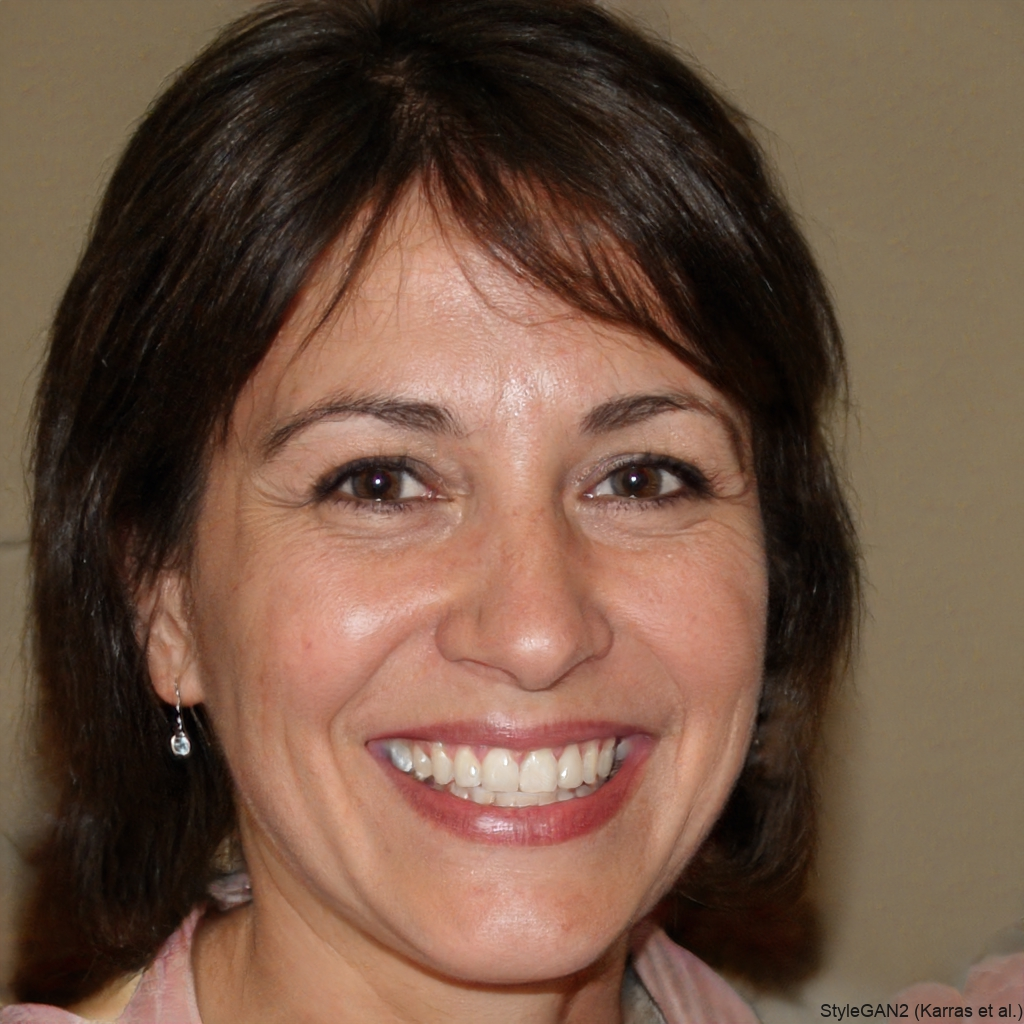
\includegraphics[width=0.32\textwidth]{introduction/figures/stylegan_example_1.jpeg}
    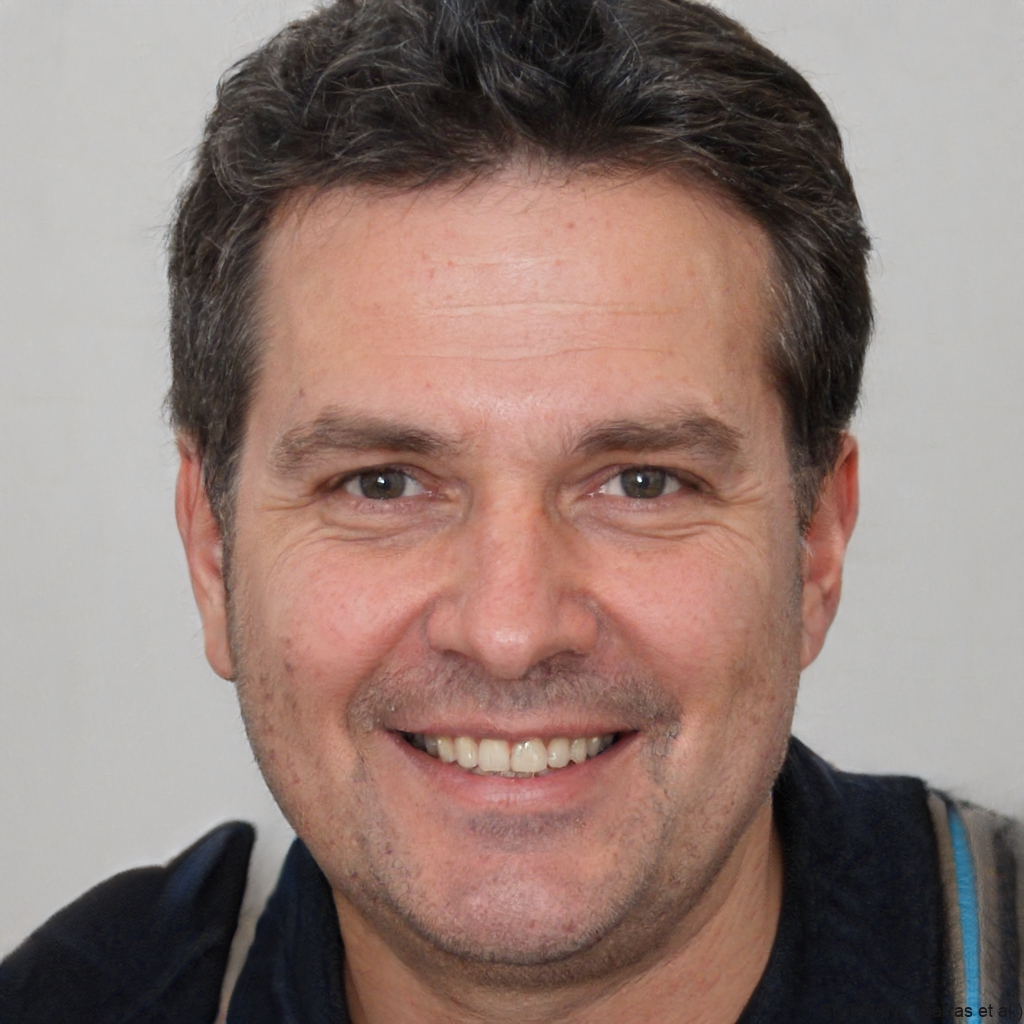
\includegraphics[width=0.32\textwidth]{introduction/figures/stylegan_example_2.jpeg}
    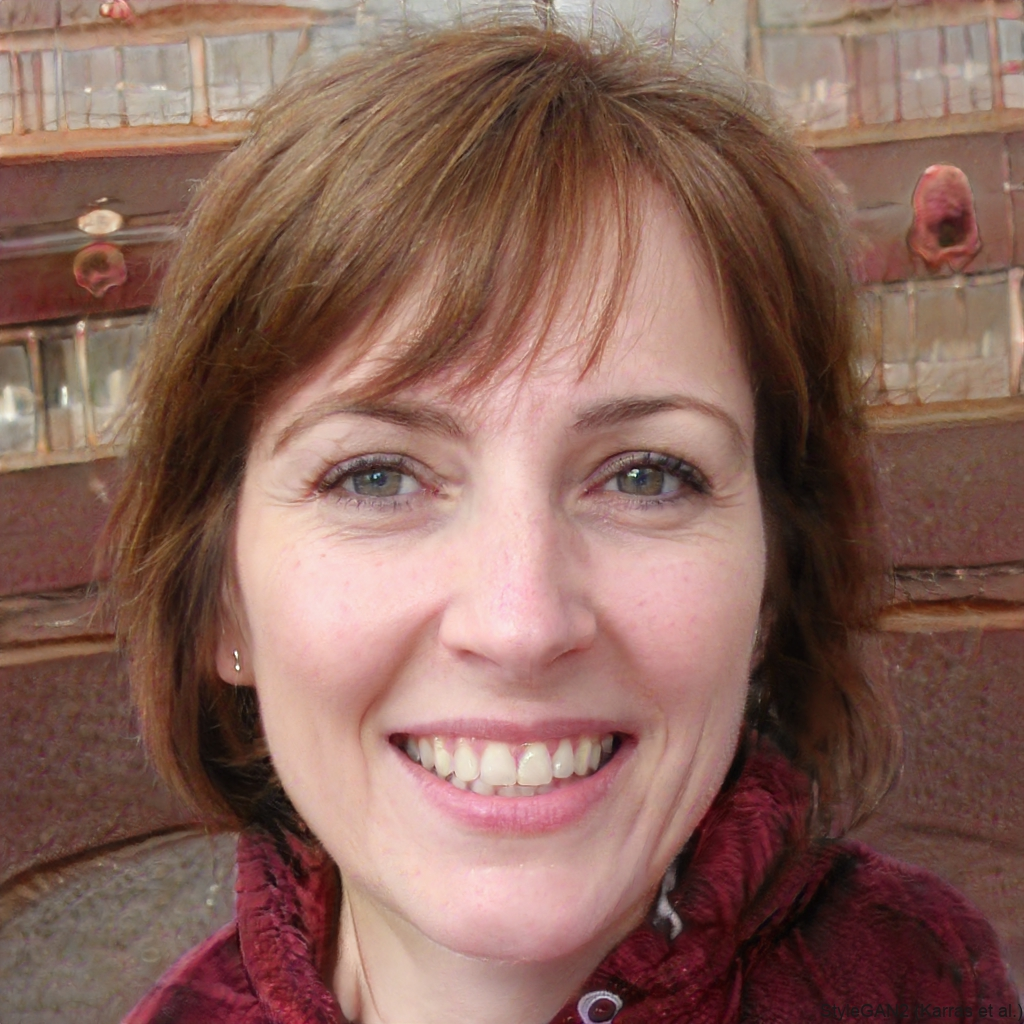
\includegraphics[width=0.32\textwidth]{introduction/figures/stylegan_example_3.jpeg}
    \caption{Samples generated by the StyleGAN model \cite{karras2019stylegan}. These high-resolution, realistic images demonstrate the capability of GANs to produce lifelike outputs.}
    \label{fig:stylegan_samples}
\end{figure}


\textsc{Weaknesses.} Despite their impressive capabilities, GANs come with a set of significant limitations that hinder their broader applicability. One of the most pressing challenges is their \textbf{training instability}, which stems from the adversarial nature of their setup. This instability often manifests in issues such as \textbf{mode collapse} \citep{arjovsky2017wasserstein}, where the generator fails to capture the diversity of the data distribution and instead produces limited varieties of samples—sometimes focusing on a single mode (see Figure~\ref{fig:mode_collapse}). This issue significantly impacts the utility of GANs, particularly in applications where diversity of the generated data is critical.

Another prominent challenge is the problem of \textbf{vanishing gradients} \citep{arjovsky2017wasserstein}. This occurs when the discriminator becomes too strong relative to the generator, leading to minimal gradient updates for the generator and stagnating its progress. Additionally, GANs are prone to \textbf{oscillatory behavior} during training, where the generator and discriminator fail to reach equilibrium, resulting in unstable or suboptimal convergence \citep{mescheder2018which}.

Moreover, GANs suffer from a fundamental limitation: they \textbf{do not provide an explicit density function} or a likelihood estimate for the generated data. This restricts their use in tasks requiring probabilistic interpretations, such as uncertainty quantification or anomaly detection, where an understanding of sample likelihoods is essential.

These challenges highlight the need for alternative or complementary generative modeling approaches, such as normalizing flows \citep{papamakarios2019normalizing} or diffusion models \citep{ho2020denoising}, which offer more stable training and explicit density estimation, enabling broader applicability and robustness across diverse tasks. However, GANs remain a valuable tool in scenarios where visual fidelity and sample quality are the primary objectives.

\begin{figure}[h!]
    \centering
    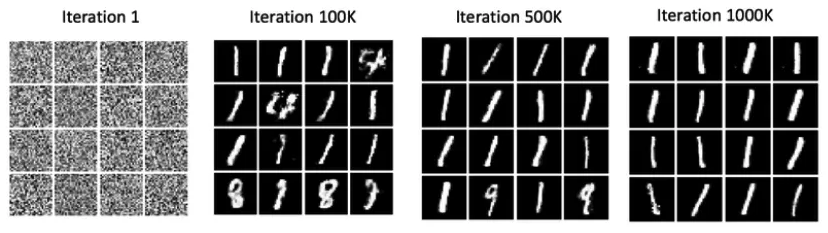
\includegraphics[width=0.8\textwidth]{introduction/figures/mode_collapse.png}
    \caption{Demonstration of mode collapse in GANs: A vanilla GAN trained on the MNIST dataset is expected to generate samples from all modes of the data distribution (i.e., all digits). However, as training progresses, the generator increasingly focuses on producing convincing samples of a single mode (i.e., the digit 1), illustrating the issue of mode collapse. This highlights the tendency of GANs to fail in capturing the diversity of the data distribution.}
    \label{fig:mode_collapse}
\end{figure}



\subsection{Variational Autoencoders (VAEs)}\label{sec:vae}

Variational Autoencoders (VAEs), introduced by \citet{kingma2013auto} and \citet{rezende2014stochastic}, are a powerful class of latent variable models. They aim to simultaneously learn a compact, low-dimensional latent representation of data and a generative process capable of synthesizing new samples. This combination makes VAEs a cornerstone of representation learning and probabilistic generative modeling.

VAEs rely on the assumption that observed data \(X \in \mathcal{X}\) is generated from unobserved latent variables \(Z \in \mathcal{Z}\) through a probabilistic generative process. This process is characterized by two key components. The latent variable \(Z\) is assumed to follow a simple prior distribution, typically a standard normal distribution:
\[
p_{Z}(\mathbf{z}) = \mathcal{N}(\mathbf{z}; \mathbf{0}, \mathbf{I}),
\]
which encourages compact and smooth representations in the latent space. The observed variable \(X\), conditioned on a latent sample \(\mathbf{z}\), follows a parameterized conditional density:
\begin{equation}
p_{X \mid Z, \theta}(\mathbf{x} \mid \mathbf{z}) = \mathcal{N}(\mathbf{x}; \mu_\theta(\mathbf{z}), \sigma_\theta^2(\mathbf{z}) \mathbf{I}),
\end{equation}\label{intro:eq:gaussian_reconstruction}

where the mean \(\mu_\theta(\mathbf{z}) \in \mathbb{R}^d\) and variance \(\sigma_\theta^2(\mathbf{z}) \in \mathbb{R}\) are outputs of a neural network (decoder) with parameters \(\theta\). These assumptions define the generative model: latent variables are sampled from the prior, and data is generated conditionally through the decoder network.

\textit{The Challenge of Marginal Likelihood Optimization.}  
The marginal log-likelihood of a data point \(\mathbf{x}\) under the stated model assumptions is given by:
\[
\log p_{X, \theta}(\mathbf{x}) = \log \int p_{X, Z, \theta}(\mathbf{x}, \mathbf{z}) \, d\mathbf{z} = \log \int p_{X \mid Z, \theta}(\mathbf{x} \mid \mathbf{z}) \, p_{Z}(\mathbf{z}) \, d\mathbf{z}.
\]

This integral is intractable because, for a given data point \(\mathbf{x}\), only a small region in the latent space \(\mathcal{Z}\) significantly contributes to the likelihood. This critical region corresponds to values of \(\mathbf{z}\) where the conditional likelihood \(p_{X \mid Z, \theta}(\mathbf{x} \mid \mathbf{z})\) is high, concentrating most of the reconstruction probability mass. Intuitively, this reflects the fact that each data point is typically explained by a specific combination of underlying generative factors, such as shape, texture, or orientation, which correspond to a small subset of the latent space. When attempting to estimate the integral using Monte Carlo sampling from the prior \(p_Z(\mathbf{z})\), the vast majority of samples fall outside this region and contribute negligibly to the likelihood. This leads to highly inefficient sampling and high-variance estimates, as reliable integration would require an impractically large number of samples.

If we could sample directly from the true posterior \(p_{Z \mid X, \theta}(\mathbf{z} \mid \mathbf{x})\), which focuses on this important region of the latent space, we could obtain reliable Monte Carlo estimates of the likelihood. However, the true posterior itself depends on the intractable marginal likelihood \(p_{X, \theta}(\mathbf{x})\), making direct computation impractical. This is where the variational approximation of the posterior comes into play.

\textit{Variational Approximation of the True Posterior.} To address this intractability, VAEs introduce a variational approximation \(q_{Z \mid X, \phi}(\mathbf{z} \mid \mathbf{x})\), modeled by a neural network (the encoder), to approximate the true posterior \(p_{Z \mid X, \theta}(\mathbf{z} \mid \mathbf{x})\). The variational distribution \(q_{Z \mid X, \phi}(\mathbf{z} \mid \mathbf{x})\) is parameterized as a Gaussian:
\[
q_{Z \mid X, \phi}(\mathbf{z} \mid \mathbf{x}) = \mathcal{N}(\mathbf{z}; \mu_\phi(\mathbf{x}), \mathrm{diag}(\sigma_\phi^2(\mathbf{x}))),
\]
where \(\mu_\phi(\mathbf{x}) \in \mathbb{R}^k\) and \(\sigma_\phi(\mathbf{x}) \in \mathbb{R}^k\) are outputs of the encoder network with parameters \(\phi\) and $k$ denotes the dimension of the latent space.

The encoder is trained to match the true posterior as closely as possible, ensuring that the critical region of the latent space is sampled effectively. This enables low-variance Monte Carlo estimates of the marginal likelihood via importance sampling. The variational approximation thus transforms an otherwise intractable optimization problem into a practical one, paving the way for the derivation of the evidence lower bound (ELBO), a tractable objective that can be efficiently optimized to jointly train the encoder and decoder.

\textit{Derivation of the Evidence Lower Bound (ELBO).} To address the intractability of directly optimizing the marginal log-likelihood \(\log p_{X,\theta}(\mathbf{x})\), the variational approximation \(q_{Z\mid X,\phi}(\mathbf{z} \mid \mathbf{x})\) is utilized. This approximation allows efficient sampling from the critical region of the latent space that contributes most to the likelihood. Rewriting the marginal log-likelihood gives:
\[
\log p_{X,\theta}(\mathbf{x}) 
\,=\,
\log 
\int 
q_{Z \mid X,\phi}(\mathbf{z} \mid \mathbf{x}) 
\frac{p_{X,Z,\theta}(\mathbf{x}, \mathbf{z})}{q_{Z \mid X,\phi}(\mathbf{z} \mid \mathbf{x})}
\, d\mathbf{z}.
\]
The term inside the integral represents an importance-weighted likelihood, where the variational distribution \(q_{Z \mid X,\phi}(\mathbf{z} \mid \mathbf{x})\) serves as the proposal distribution for efficiently sampling from the posterior. 

Applying Jensen's inequality to the logarithm of the expectation yields:
\[
\log p_{X,\theta}(\mathbf{x}) 
\,\geq\,
\mathbb{E}_{q_{Z \mid X,\phi}(\mathbf{z} \mid \mathbf{x})} 
\left[
\log \frac{p_{X,Z,\theta}(\mathbf{x}, \mathbf{z})}{q_{Z \mid X,\phi}(\mathbf{z} \mid \mathbf{x})}
\right].
\]
The right-hand side is defined as the \emph{Evidence Lower Bound} (ELBO), denoted as \(\mathrm{ELBO}(\theta, \phi)\). By construction, the ELBO provides a tractable lower bound on the marginal log-likelihood and serves as the objective for training VAEs. Substituting the joint probability \(p_{X,Z,\theta}(\mathbf{x}, \mathbf{z}) = p_{X \mid Z,\theta}(\mathbf{x} \mid \mathbf{z}) \, p_Z(\mathbf{z})\), the ELBO can be expressed as:
\[
\mathrm{ELBO}(\theta, \phi) 
\,=\,
\mathbb{E}_{q_{Z \mid X,\phi}(\mathbf{z} \mid \mathbf{x})}
\big[
\log p_{X \mid Z,\theta}(\mathbf{x} \mid \mathbf{z})
\big]
\;-\;
D_{\mathrm{KL}}
\big(q_{Z \mid X,\phi}(\mathbf{z} \mid \mathbf{x}) \,\|\, p_Z(\mathbf{z})\big).
\]

\noindent The ELBO consists of two terms:
\begin{enumerate}
    \item \textbf{Reconstruction Term:}  
    \[
    \mathbb{E}_{q_{Z \mid X,\phi}(\mathbf{z} \mid \mathbf{x})} 
    \big[\log p_{X \mid Z,\theta}(\mathbf{x} \mid \mathbf{z})\big],
    \]
    which encourages the generative model \(p_{X \mid Z,\theta}\) (decoder) to reconstruct the observed data \(\mathbf{x}\) accurately from the latent representation \(\mathbf{z}\).
    \item \textbf{KL Divergence Term:}  
    \[
    D_{\mathrm{KL}}(q_{Z \mid X,\phi}(\mathbf{z} \mid \mathbf{x}) \,\|\, p_Z(\mathbf{z})),
    \]
    which regularizes the approximate posterior \(q_{Z \mid X,\phi}\), ensuring that the learned latent representations are close to the prior \(p_Z\).
\end{enumerate}

Together, these terms balance accurate data reconstruction and latent space regularization. Maximizing the ELBO ensures the latent space encodes meaningful, generalizable representations while enabling robust reconstruction through the decoder.

\textit{Connection to the Marginal Log-Likelihood.} To further understand the role of the ELBO, the marginal log-likelihood can be decomposed as follows:
\[
\log p_{X,\theta}(\mathbf{x}) 
\,=\,
\mathrm{ELBO}(\theta, \phi)
\,+\,
D_{\mathrm{KL}}\big(q_{Z \mid X,\phi}(\mathbf{z} \mid \mathbf{x}) \,\|\, p_{Z \mid X,\theta}(\mathbf{z} \mid \mathbf{x})\big).
\]
The second term is the KL divergence between the approximate posterior \(q_{Z \mid X,\phi}\) and the true posterior \(p_{Z \mid X,\theta}\). This term is always non-negative, implying that \(\mathrm{ELBO}(\theta, \phi) \leq \log p_{X,\theta}(\mathbf{x})\). From this decomposition, it additionally becomes clear that maximizing the ELBO serves a dual purpose:
\begin{enumerate}
    \item It increases the lower bound on the marginal log-likelihood, improving the model's ability to explain the data.
    \item It minimizes the mismatch between the approximate posterior \(q_{Z \mid X,\phi}\) and the true posterior \(p_{Z \mid X,\theta}\), ensuring effective latent representation learning.
\end{enumerate}



\textsc{Training Objective.} The training objective of Variational Autoencoders (VAEs) extends from the Evidence Lower Bound (ELBO), balancing reconstruction accuracy and latent space regularization. The goal is to maximize the ELBO or equivalently minimize its negative form:
\[
\mathcal{L}_{\text{VAE}}(\theta, \phi)
\;=\;
-\,\mathbb{E}_{q_{Z \mid X,\phi}(\mathbf{z}\mid \mathbf{x})}\!
\bigl[\log p_{X \mid Z, \theta}(\mathbf{x}\mid \mathbf{z})\bigr]
\;+\;
D_{\mathrm{KL}}\!\Bigl(
    q_{Z \mid X,\phi}(\mathbf{z}\mid \mathbf{x})
    \,\bigl\|\,
    p_{Z}(\mathbf{z})
\Bigr).
\]

\noindent Under the Gaussian decoder assumption presented in Equation~\ref{intro:eq:gaussian_reconstruction}, where:
\[
p_{X \mid Z, \theta}(\mathbf{x} \mid \mathbf{z}) = \mathcal{N}(\mathbf{x}; \mu_\theta(\mathbf{z}), \sigma_\theta^2(\mathbf{z}) \mathbf{I}),
\]
the log-likelihood term in the \(\mathcal{L}_{\text{VAE}}\) objective simplifies to an \(\ell^2\) reconstruction term:
\[
-\mathbb{E}_{q_{Z \mid X, \phi}(\mathbf{z} \mid \mathbf{x})}
\bigl[\log p_{X \mid Z, \theta}(\mathbf{x} \mid \mathbf{z})\bigr]
\;=\;
\frac{1}{2\sigma_\theta^2}\mathbb{E}_{q_{Z \mid X, \phi}(\mathbf{z} \mid \mathbf{x})}
\bigl[\|\mathbf{x} - \mu_\theta(\mathbf{z})\|^2\bigr]
+ \text{const}.
\]

In most practical implementations, \(\sigma_\theta\) is set to 1, simplifying the the trainining objective to:
\[
\mathcal{L}_{\text{VAE}}(\theta, \phi)
\;=\;
\mathbb{E}_{q_{Z \mid X, \phi}(\mathbf{z} \mid \mathbf{x})}
\bigl[\|\mathbf{x} - \mu_\theta(\mathbf{z})\|^2\bigr]
\;+\;
D_{\mathrm{KL}}\!\Bigl(
    q_{Z \mid X,\phi}(\mathbf{z}\mid \mathbf{x})
    \,\bigl\|\,
    p_{Z}(\mathbf{z})
\Bigr).
\]

The first term ensures accurate reconstruction, while the second term regularizes the latent space to stay close to the prior \(p_Z\). Together, these terms balance generative performance and the compactness of the learned latent space. Optimization is made efficient using stochastic gradient descent and the \emph{reparameterization trick} \citep{kingma2013auto}.

To provide more control over the trade-off between reconstruction and regularization, the \(\beta\)-ELBO \citep{higgins2017beta} introduces a weighting factor \(\beta > 0\) for the KL term:
\[
\mathcal{L}_{\beta\text{-VAE}}(\theta, \phi)
\;=\;
\mathbb{E}_{q_{Z \mid X, \phi}(\mathbf{z} \mid \mathbf{x})}
\bigl[\|\mathbf{x} - \mu_\theta(\mathbf{z})\|^2\bigr]
\;+\;
\beta \, D_{\mathrm{KL}}\!\Bigl(
    q_{Z \mid X,\phi}(\mathbf{z}\mid \mathbf{x})
    \,\bigl\|\,
    p_{Z}(\mathbf{z})
\Bigr).
\]

The \(\beta\)-ELBO provides a flexible framework to adapt VAEs for diverse tasks by adjusting the trade-off between reconstruction and regularization. When \(\beta = 1\), the objective reduces to the standard ELBO. For \(\beta < 1\), the reconstruction term is prioritized by underweighting regularization, improving reconstruction quality but potentially compromising latent space structure. Conversely, \(\beta > 1\) enforces stronger regularization, which can promote disentanglement in the latent space but may reduce reconstruction fidelity. This flexibility allows the \(\beta\)-ELBO to balance generative performance with latent structure, making \(\beta\)-VAEs well-suited for a wide range of applications.

\textsc{Sampling and Distribution Mismatch.} Once trained, the model can generate new samples \(\mathbf{x}_{\text{new}}\) by first drawing \(\mathbf{z} \sim P(Z)\) (e.g., \(\mathcal{N}(\mathbf{0}, \mathbf{I})\)) and then sampling \(\mathbf{x}_{\text{new}} \sim p_{\theta}(X \mid Z)\). However, in practice, the \emph{aggregated posterior}
\[
q_{Z}(\mathbf{z}) 
\;=\;
\int
q_{Z \mid X,\phi}(\mathbf{z}\mid \mathbf{x})
\;p_{X}(\mathbf{x})
\;d\mathbf{x}
\]
often differs from \(p_{Z}(\mathbf{z})\). This mismatch can result in poor-quality samples if we draw \(\mathbf{z}\) directly from the prior distribution, because the decoder rarely “sees” latent codes that lie far outside the support of \(q_{Z}(\mathbf{z})\).

\textsc{VAEs in Combination with Other Generative Models.} To alleviate this mismatch, VAEs are frequently combined with other frameworks that can accurately model the aggregated posterior density \(q_{Z}(\mathbf{z})\). For instance, \textit{latent diffusion models} \cite{rombach2022high} are employed to model the aggregated posterior distribution. Here, the VAE’s encoder compresses high-dimensional data \(\mathbf{x}\) into a latent representation \(\mathbf{z}\), and a diffusion model is trained to model \(q_{Z}(\mathbf{z})\). At sampling time, the diffusion model generates \(\mathbf{z}\) in the compressed space, and the VAE’s decoder then reconstructs a high-resolution sample in \(\mathcal{X}\). This factorization into a \emph{learned, lower-dimensional space} significantly reduces the computational cost of training and sampling while often improving sample fidelity.

\textsc{Strengths.} VAEs are a powerful framework that seamlessly combines generative modeling and representation learning, excelling in both domains. They provide \textbf{compact, semantically meaningful latent representations} that enable tasks such as data interpolation, clustering, and feature extraction, making them particularly effective for analyzing and manipulating high-dimensional data. Simultaneously, their generative capabilities allow for synthesizing \textbf{high-quality samples from the latent space}, with the probabilistic framework naturally incorporating uncertainty—a valuable property for anomaly detection, Bayesian inference, and robust decision-making under uncertainty. Unlike adversarial models like GANs, VAEs rely on the ELBO objective, ensuring \textbf{stable training} without issues like mode collapse. This stability, coupled with their \textbf{flexibility}, enables VAEs to integrate seamlessly with advanced generative techniques such as latent diffusion models, enhancing sample fidelity and computational efficiency, especially in high-dimensional settings. These strengths position VAEs as a versatile and foundational tool for a wide range of applications in modern machine learning.

\textsc{Weaknesses.} Despite their strengths, VAEs face notable challenges that limit their generative performance. A primary issue is the tendency to produce \textbf{blurred reconstructions and samples}, stemming from the Gaussian decoder assumption, which simplifies the conditional likelihood and constrains the model's ability to capture complex data structures. This limitation is illustrated in Figure~\ref{fig:vae_blur_reconstructions}, where we observe that the reconstructions generated by a standard VAE fail to retain fine-grained details present in the original images. 

\begin{figure}[h]
    \centering
    % Original images
    \begin{minipage}{\textwidth}
        \centering
        \foreach \d in {2,3,4,5,6,7} {
            \includegraphics[width=0.14\textwidth]{introduction/figures/vae/original/\d.png}
        }
        \\[0.5ex] % Add spacing
        Original images
    \end{minipage}
    \\[1ex] % Vertical space between original and reconstructed images
    % Reconstructed images
    \begin{minipage}{\textwidth}
        \centering
        \foreach \d in {2,3,4,5,6,7} {
            \includegraphics[width=0.14\textwidth]{introduction/figures/vae/reconstruction/\d.png}
        }
        \\[0.5ex] % Add spacing
        Reconstructed images
    \end{minipage}
    \caption{
        Comparison of original images (top row) and VAE reconstructions (bottom row), highlighting the \textbf{blurring effect} caused by the Gaussian decoder assumption, which limits the VAE's ability to capture fine details and complex structures.
    }
    \label{fig:vae_blur_reconstructions}
\end{figure}

This limitation is addressed in chapter \ref{Chapter:ScoreVAE}, where we introduce \textit{ScoreVAE}, a novel adaptation of the VAE framework. By combining a diffusion-time-dependent encoder with an unconditional diffusion model and leveraging Bayes' rule for score functions, \textit{ScoreVAE} bypasses the Gaussian assumption and provides a more expressive reconstruction distribution, significantly enhancing the model's ability to capture intricate high-dimensional structures. 

Additionally, the \textbf{mismatch between the aggregated posterior and the prior}, which often leads to poor-quality samples, necessitates a model that learns the aggregated posterior distribution, such as a latent diffusion model or a latent normalizing flow, to improve sample fidelity and better align the generative process with the learned latent space.




\subsection{Normalizing Flows}\label{sec:normalizing_flows}

Normalizing flows, introduced by Rezende and Mohamed \cite{rezende2015variational}, are a versatile class of generative models that provide a unified framework for both data generation and explicit likelihood estimation. These models transform a simple base distribution into a complex target distribution using a sequence of invertible and differentiable mappings, enabling exact computation of likelihoods. Normalizing flows are trained by directly maximizing the log-likelihood of the observed data, leveraging the change of variables formula to compute densities in closed form. This combination of flexibility, tractability, and theoretical soundness makes normalizing flows a powerful tool for modeling complex probability distributions.

Given a latent variable $Z \sim P(Z)$ in latent space $\mathcal{Z}$ and an invertible function $G^\theta: \mathcal{Z} \rightarrow \mathcal{X}$ parameterized by $\theta$, the model defines the random variable $X = G^\theta(Z)$ in data space $\mathcal{X}$ to approximate the data distribution $P(X)$. The transformation $G^\theta$ maps samples from the base distribution to samples resembling the observed data.

To compute the probability density function (pdf) of $X$, the change of variables formula is employed. For an invertible and differentiable transformation $G^\theta$, with inverse $F^\theta = (G^\theta)^{-1}$, the pdf of $X$ is given by:

\[
p^\theta_X(\mathbf{x}) = p_Z\left(F^\theta(\mathbf{x})\right) \left| \det \left( \frac{\partial F^\theta(\mathbf{x})}{\partial \mathbf{x}} \right) \right|,
\]

\noindent where $\frac{\partial F^\theta(\mathbf{x})}{\partial \mathbf{x}}$ is the Jacobian matrix of $F^\theta$ at point $\mathbf{x}$, and $\det$ denotes the determinant. Taking the logarithm yields:

\[
\log p^\theta_X(\mathbf{x}) = \log p_Z\left(F^\theta(\mathbf{x})\right) + \log \left| \det \left( \frac{\partial F^\theta(\mathbf{x})}{\partial \mathbf{x}} \right) \right|.
\]

This formulation enables exact computation of the log-likelihood, which is crucial for effective training.

In practice, the transformation $G^\theta$ is constructed by composing a sequence of $K$ invertible and differentiable transformations:

\[
G^\theta = G_K \circ G_{K-1} \circ \dots \circ G_1,
\]

\noindent where each $G_k$ is an invertible function. The inverses of these transformations are denoted as $F_k = G_k^{-1}$.

\noindent For a data point $\mathbf{x}$, intermediate variables are defined by recursively applying the inverses:

\[
\mathbf{h}_0 = \mathbf{x}, \quad \mathbf{h}_k = F_k(\mathbf{h}_{k-1}), \quad \text{for } k = 1, \dots, K.
\]

\noindent The log-density of $\mathbf{x}$ can then be expressed as:

\[
\log p^\theta_X(\mathbf{x}) = \log p_Z(\mathbf{h}_K) + \sum_{k=1}^{K} \log \left| \det \left( \frac{\partial F_k(\mathbf{h}_{k-1})}{\partial \mathbf{h}_{k-1}} \right) \right|.
\]

A crucial aspect of designing normalizing flows is ensuring that the composing functions \( G_k \) are, typically, analytically invertible to allow for fast sampling. Additionally, the calculation of the determinant of the Jacobian must be tractable to enable efficient training via the change of variables formula. This is often achieved by designing the transformations so that the resulting Jacobian matrices have a lower triangular form or another structure that simplifies the computation of the determinant. By constructing \( G_k \) in this manner, normalizing flows facilitate efficient evaluation of both the forward and inverse transformations, as well as the log-determinant of the Jacobian, thereby enabling effective training and fast sampling from the model.

\textsc{Training Objective.} The parameters $\theta$ of the normalizing flow are optimized by maximizing the likelihood of the observed data $\{\mathbf{x}_i\}_{i=1}^N$, which is equivalent to minimizing the negative log-likelihood:

\[
\theta^* = \arg \min_{\theta} \sum_{i=1}^N -\log p^\theta_X(\mathbf{x}_i).
\]

By leveraging the exact computation of the log-likelihood, normalizing flows can be trained using standard gradient-based optimization methods, ensuring stable and efficient convergence.

\textsc{Strengths.} Normalizing flows offer several advantages. A primary strength is their ability to perform \textbf{exact density computation}, allowing for tractable and exact likelihood evaluations. This facilitates stable training via maximum likelihood estimation \cite{papamakarios2019normalizing}. Furthermore, they provide \textbf{efficient sampling}; once trained, new samples can be generated rapidly by transforming latent samples through \( G^\theta \). The analytical invertibility of \( G^\theta \) and efficient computation of Jacobian determinants make both training and sampling computationally efficient.

\textsc{Weaknesses.} Despite their strengths, normalizing flows have limitations. The requirement for invertibility and tractable Jacobians imposes constraints on the choice of transformations, potentially leading to \textbf{limited expressivity} \cite{papamakarios2019normalizing}. This can hinder the model's ability to capture complex data distributions, especially those with intricate structures. Additionally, normalizing flows can encounter \textbf{topological limitations and numerical stability issues} when modeling targets with complicated topologies. In such cases, the model may become numerically non-invertible to approximate the target distribution closely, leading to stability problems and reducing the effectiveness of the flow \cite{behrmann2021understanding, cornish2020relaxing}. 

Normalizing flows, while powerful, \textbf{lack a semantically meaningful lower-dimensional latent space}, unlike GANs and Variational Auto-Encoders (VAEs). GANs and VAEs are designed with a lower-dimensional latent space, explicitly chosen a priori, enabling their effective use in downstream tasks such as compression, image-text alignment, and editing. In contrast, the latent space of normalizing flows is inherently tied to the ambient space's dimensionality, limiting its direct interpretability. In chapter \ref{Chapter:Pullback-riemannian-geometry}, we address this limitation by adapting normalizing flows to acquire an interpretable latent space. Our approach combines an anisotropic base distribution with isometry regularization, drawing on principles from pullback Riemannian geometry. This training paradigm constructs a latent space where semantic significance is encoded by the variances learned in the base distribution. Latent dimensions capturing meaningful semantic information are characterized by high variances, while those encoding noise exhibit very low variance, enabling a clear distinction between essential and extraneous information.

\subsection{Auto-Regressive Models}\label{sec:auto_regressive_models}

Auto-regressive models are a class of generative models that factorize the joint probability density of high-dimensional data into a product of conditional densities, leveraging the chain rule of probability. Notable examples include PixelCNN and PixelRNN \cite{oord2016pixel}, WaveNet \cite{vanwavenet2016}, and more recently, Transformer-based models \cite{vaswani2017attention}, which have been applied across various domains such as natural language processing, image generation, and audio synthesis.

Given a data vector \( \mathbf{x} = [x_1, x_2, \dots, x_d] \) in \( \mathbb{R}^d \), the joint density \( p_X(\mathbf{x}) \) is decomposed into a product of conditional densities:

\[
p_X(\mathbf{x}) = p_{X_1}(x_1) \prod_{i=2}^{d} p_{X_i \mid X_{1:i-1}}(x_i \mid x_{1:i-1}),
\]

\noindent where \( p_{X_1}(x_1) \) represents the marginal probability of the first variable, \( X_{1:i-1} \) denotes all preceding random variables in a predefined ordering, and \( x_{1:i-1} \) represents their corresponding realizations. This factorization enables the model to capture complex dependencies between variables by modeling each variable conditioned on all previous ones.

Each conditional density \( p_{X_i \mid X_{1:i-1}}(x_i \mid x_{1:i-1}) \) is modeled using a neural network that takes \( x_{1:i-1} \) as input and outputs the parameters of the density for \( x_i \). For instance, in PixelCNN, convolutional neural networks with masked filters are employed to ensure that the prediction of a pixel \( x_i \) depends only on pixels \( x_{1:i-1} \) that come before it in the chosen ordering.

The masking technique is critical; it zeroes out connections in the network to prevent information from "future" variables influencing the prediction of the current variable, thus maintaining the auto-regressive property.

\textsc{Training Objective.} The parameters \( \theta \) of the auto-regressive model are optimized by maximizing the likelihood of the observed data \( \{\mathbf{x}_n\}_{n=1}^N \), which is equivalent to minimizing the negative log-likelihood:

\[
\begin{aligned}
\theta^* &= \arg \min_{\theta} \sum_{n=1}^{N} -\log p_{X,\theta}(\mathbf{x}_n) \\
         &= \arg \min_{\theta} \sum_{n=1}^{N} \left[ -\log p_{X_1,\theta}(x_{n,1}) 
         + \sum_{i=2}^{d} -\log p_{X_i \mid X_{1:i-1}, \theta}(x_{n,i} \mid x_{n,1:i-1}) \right],
\end{aligned}
\]

\noindent where \( x_{n,i} \) represents the \( i \)-th variable in the \( n \)-th observed data sample, and \( x_{n,1:i-1} \) denotes its preceding realizations. The inclusion of \( p_{X_1,\theta}(x_{n,1}) \) accounts for the marginal probability of the first variable, ensuring the complete factorization of the joint likelihood.

\textsc{Sampling Process.} Sampling from auto-regressive models is inherently sequential. To generate a new data sample \( \mathbf{x} \), the model starts by sampling \( x_1 \) from \( p_{X_1}(x_1) \). Then, for \( i = 2 \) to \( d \), each \( x_i \) is sampled from \( p_{X_i \mid X_{1:i-1}}(x_i \mid x_{1:i-1}) \), using the previously sampled values. This process continues until all variables have been generated.

\textsc{Strengths.} Auto-regressive models have several notable strengths. A primary advantage is their ability to perform \textbf{exact likelihood computation}, providing an exact calculation of the data likelihood without any approximation. This facilitates stable training via maximum likelihood estimation, ensuring that the model accurately captures the underlying data density. Additionally, by conditioning each variable on all previous ones, auto-regressive models are highly effective at \textbf{modeling complex dependencies} in sequential or structured data. This makes them particularly well-suited for tasks such as language modeling, image generation, and audio synthesis, where capturing intricate patterns and dependencies is crucial. Furthermore, auto-regressive models offer \textbf{flexibility in handling different data types}; they can model both discrete and continuous data by appropriately choosing the form of the conditional densities, such as using categorical densities for discrete variables or Gaussian densities for continuous ones.

\textsc{Weaknesses.} Despite these strengths, auto-regressive models also present significant weaknesses. A major limitation is the \textbf{slow sampling process} inherent in their sequential nature. Generating a single data sample requires sampling each variable one at a time, conditioned on the previously generated variables. This makes the sampling process computationally intensive and time-consuming, especially for high-dimensional data like high-resolution images or long sequences, where the number of variables \( d \) is large. Moreover, the sequential dependency of variables \textbf{limits parallelization during sampling}, as each variable depends on the outcome of the previous ones, preventing the use of parallel computation techniques to speed up sample generation. This can be particularly problematic when rapid generation of many samples is required.


\subsection{Energy-Based Models (EBMs)}\label{sec:energy_based_models}

Energy-Based Models (EBMs) \cite{lecun2006tutorial} define an unnormalized probability density over data using an energy function \( E_\theta(\mathbf{x}) \). The density of a data point \( \mathbf{x} \in \mathcal{X} \) is given as:
\[
p_\theta(\mathbf{x}) = \frac{\exp(-E_\theta(\mathbf{x}))}{Z_\theta},
\]
where \( Z_\theta = \int_{\mathcal{X}} \exp(-E_\theta(\mathbf{x})) \, d\mathbf{x} \) is the partition function, a normalizing constant that ensures \( p_\theta(\mathbf{x}) \) integrates to 1 over \( \mathcal{X} \). However, computing \( Z_\theta \) is typically intractable for high-dimensional data, posing challenges for direct optimization and sampling.

\textsc{Training Objective.} EBMs are trained to assign low energy values to samples drawn from the data distribution (positive samples) and high energy values to samples from the model distribution (negative samples). A commonly used training objective is based on contrastive divergence \cite{hinton2002training}, which minimizes the expected energy of positive samples while maximizing the expected energy of negative samples:
\[
\mathcal{L}(\theta) = \mathbb{E}_{X^+ \sim P(X)} [E_\theta(X^+)] - \mathbb{E}_{X^- \sim P_\theta(X)} [E_\theta(X^-)],
\]
where \( X^+ \) and \( X^- \) are random variables associated with the data distribution \( P(X) \) and the model distribution \( P_\theta(X) \), respectively. 

To obtain negative samples \(\mathbf{x}^-\), a standard approach is to use \textit{Markov Chain Monte Carlo (MCMC)} methods, with Langevin Dynamics \cite{langevin1908theorie, neal2011mcmc} being a widely adopted technique. Langevin Dynamics is a stochastic gradient-based method that iteratively updates a sample \(\mathbf{x}_t\) to move toward regions of higher probability density under the unnormalized model density \(p_\theta(\mathbf{x})\). The iterative update rule is given by:

\[
\mathbf{x}_{t+1} \;=\; \mathbf{x}_t \;-\; \eta\,\nabla_{\mathbf{x}} E_\theta\bigl(\mathbf{x}_t\bigr) \;+\; \sqrt{2\eta}\,\boldsymbol{\epsilon}_t,
\]

\noindent where \(\eta>0\) is the step size, and \(\boldsymbol{\epsilon}_t \sim \mathcal{N}(\mathbf{0}, I)\) represents Gaussian noise added to incorporate stochasticity into the updates. The term \(-\nabla_{\mathbf{x}} E_\theta(\mathbf{x}_t)\) drives \(\mathbf{x}_t\) toward regions of lower energy, while the stochastic noise \(\boldsymbol{\epsilon}_t\) prevents the chain from getting trapped in local minima.

This approach ensures that the generated negative samples \(\mathbf{x}^-\) align with the model's current energy landscape. The addition of noise also maintains ergodicity, which is crucial for exploring the sample space. In the limit of small step sizes \(\eta\) and sufficient iterations, the chain converges to the target distribution \(P_\theta(X)\).

\textsc{Sampling Process.} Sampling from EBMs follows the same procedure as obtaining negative samples. Since direct sampling is infeasible due to the intractability of \( Z_\theta \), MCMC methods like Langevin Dynamics are used to approximate samples from the target distribution \( P_\theta(X) \). This iterative process converges to high-density regions of \( P_\theta(X) \), making it suitable for generation tasks. However, the need for multiple iterations results in a slow sampling process, particularly for high-dimensional data.

\textsc{Strengths.} EBMs offer several notable strengths. One of their primary advantages is their \textbf{flexibility} in representing complex distributions without requiring explicit normalization, as they define an unnormalized probability distribution directly using an energy function \cite{lecun2006tutorial}. This flexibility allows EBMs to focus on modeling the energy landscape of the data, making them highly adaptable to diverse data types and problem settings. Unlike other generative models, such as GANs or normalizing flows, which often require specific assumptions about the form of the probability distribution or rely on explicit normalization, EBMs can represent distributions of arbitrary complexity by appropriately designing the energy function.

Furthermore, EBMs exhibit strong \textbf{compositionality}, allowing seamless integration with other models and the incorporation of domain-specific knowledge such as constraints or priors \cite{du2019implicit, grathwohl2020your}. This property enables EBMs to handle applications requiring hybrid generative processes or strict adherence to domain rules. By encoding physical laws or chemical properties directly into the energy function, EBMs can generate outcomes that comply with these constraints, making them particularly effective in scientific modeling tasks like physical simulations and molecular design \cite{du2019implicit}. In structured prediction tasks, EBMs can impose priors to ensure outputs follow specific patterns or relationships, such as spatial coherence in semantic segmentation or hierarchical structures in knowledge graph synthesis \cite{grathwohl2020your, lecun2006tutorial}. This compositional and flexible nature allows EBMs to excel in applications requiring constrained generative modeling or the integration of domain knowledge, where conventional generative models may struggle.

\textsc{Weaknesses.} Despite their strengths, EBMs also face significant weaknesses. A major challenge is their \textbf{training difficulty}, primarily due to the reliance on MCMC methods for generating negative samples. MCMC sampling is computationally intensive, can suffer from slow convergence, and often requires careful tuning to ensure effective exploration of the energy landscape. Additionally, EBMs exhibit \textbf{slow sampling speed}, as generating a single sample requires running iterative Langevin Dynamics or similar methods, which involve multiple gradient evaluations. This can hinder the scalability of EBMs for tasks requiring large-scale generation.


\subsection{Diffusion Models}

Denoising Diffusion Probabilistic Models (DDPMs) \cite{ho2020denoising} and score-based generative models (SGMs) \cite{song2021sde} generate data by reversing a noise corruption process. These models consist of two complementary components: a forward process that gradually perturbs data into a simple noise-like prior distribution (e.g., \( \mathcal{N}(0, \mathbf{I}) \)) and a reverse process that progressively removes the noise, converting samples from the prior distribution into realistic data samples.

In the literature, discrete-time models such as DDPMs are widely referred to as "diffusion models", a term reflecting their reliance on discrete diffusion processes to corrupt data over a finite number of steps and then reverse this transformation. Continuous-time frameworks like SGMs, on the other hand, are often described as "score-based generative models," as they emphasize the estimation of the score function—the gradient of the log probability density—and use it to define the reverse process via stochastic differential equations (SDEs). These terminologies reflect the historical development of the two frameworks, with DDPMs rooted in discrete Markov chains and SGMs in score-matching and continuous-time diffusion processes.

In this thesis, both frameworks are unified under the term "diffusion models". This unified terminology highlights the fundamental insight that DDPMs and SGMs represent two perspectives of the same underlying framework, differing only in their treatment of time as discrete or continuous. As will be shown and discussed, these frameworks are mathematically equivalent in the limit of infinite time steps. Adopting this perspective highlights their shared theoretical foundation, bridging the discrete and continuous-time paradigms, and provides a cohesive framework for exploring their principles and applications throughout this work.

\textit{Forward Process.} The forward process in diffusion and score-based generative models progressively corrupts the original data into noise, providing the foundation for learning the reverse process that generates data from noise. The design of the forward process ensures that over time, the data distribution transitions smoothly into a simple, analytically tractable distribution $\pi$, such as \( \mathcal{N}(0, \mathbf{I}) \).

\begin{itemize}
    \item \textbf{DDPM (Discrete Time):}
    
    In the Denoising Diffusion Probabilistic Model (DDPM), the forward process is a Markov chain that adds Gaussian noise to the data at discrete time steps \( t = 1, 2, \dots, N \). The transition kernel is given by:
    \[
    q_{X_t \mid X_{t-1}}(\mathbf{x}_t \mid \mathbf{x}_{t-1}) = \mathcal{N}\bigl(\mathbf{x}_t;\, \sqrt{\alpha_t} \, \mathbf{x}_{t-1},\, \beta_t \mathbf{I}\bigr),
    \]
    where:
    \begin{itemize}
        \item \( \alpha_t = 1 - \beta_t \), the scaling factor applied to \( \mathbf{x}_{t-1} \),
        \item \( \beta_t \in (0, 1) \), the predefined variance schedule controlling the amount of noise at step \( t \),
    \end{itemize}
    This formulation allows the process to be expressed in terms of the initial data \( \mathbf{x}_0 \):
    \[
    q_{X_t|X_0}(\mathbf{x}_t \mid \mathbf{x}_0) = \mathcal{N}\left(\mathbf{x}_t;\, \sqrt{\bar{\alpha}_t} \, \mathbf{x}_0,\, (1 - \bar{\alpha}_t) \mathbf{I}\right),
    \]
    where \( \bar{\alpha}_t = \prod_{s=1}^t \alpha_s \) is the cumulative product of \( \alpha_s \). This closed-form expression simplifies training and allows direct sampling from any step \( t \).

    \item \textbf{SGM (Continuous Time):} The forward process in Score-Based Generative Models (SGM) is described by a continuous-time Stochastic Differential Equation (SDE) that progressively perturbs the data distribution with infinitesimal noise:

\[
dX_t = f(X_t, t) \, dt + g(t) \, dW_t,
\]

where:
\begin{itemize}
    \item \( W_t \) is a standard Wiener process (Brownian motion),
    \item \( f(X_t, t) \) is the drift coefficient, defining the deterministic evolution of the data distribution,
    \item \( g(t) \) is the diffusion coefficient, controlling the scale of the stochastic noise.
\end{itemize}

The drift and diffusion coefficients \( f(X_t, t) \) and \( g(t) \) are carefully chosen so that, after a sufficiently large diffusion time \( T \), the data distribution evolves into a distribution that is very close to a simple, analytically tractable distribution, typically the standard normal distribution \( \mathcal{N}(\mathbf{0}, \mathbf{I}) \).

Popular choices for the forward SDE include: 

    
\begin{itemize}
    \item \textbf{Variance Preserving (VP) SDE:}
    \[
    f(X_t, t) = -\frac{1}{2} \beta(t) X_t, \quad g(t) = \sqrt{\beta(t)},
    \]
    where \( \beta(t) \) is a predefined noise schedule that controls the rate of diffusion. This choice preserves the variance of the data distribution throughout the process. The limiting distribution as \( t \to \infty \) is the standard normal distribution. In practice, after sufficient diffusion time \( T \), the perturbed distribution \( p_{X_T} \approx \mathcal{N}(\mathbf{0}, \mathbf{I}) \).
    
    \item \textbf{Variance Exploding (VE) SDE:}
    \[
    f(X_t, t) = \mathbf{0}, \quad g(t) = \sqrt{\frac{d[\sigma^2(t)]}{dt}},
    \]
    where \( \sigma(t) \) is a monotonically increasing function that scales the noise over time. In this formulation, the variance of the data distribution "explodes." After sufficient diffusion time \( T \), the perturbed distribution \( p_{X_T} \approx \mathcal{N}(\mathbf{0}, \sigma(T)^2 \mathbf{I}) \).
\end{itemize}

\end{itemize}

These formulations ensure a smooth progression from the data distribution to the prior, providing a well-defined framework for the reverse process to reconstruct data from noise.


\textit{Reverse Process.} The reverse process reconstructs the original data distribution by inverting the forward process, progressively removing noise to generate data samples:

\begin{itemize}
    \item \textbf{DDPM (Discrete Time):}
    The reverse process in DDPMs is a Markov chain that progressively denoises the data at each step. The conditional distribution for each step is expressed as:
    \[
    p_{X_{t-1} \mid X_t, \theta}(\mathbf{x}_{t-1} \mid \mathbf{x}_t) = \mathcal{N}\bigl(\mathbf{x}_{t-1}; \mu_\theta(\mathbf{x}_t, t), \beta_t^2 \mathbf{I}\bigr),
    \]
    where \( \mu_\theta(\mathbf{x}_t, t) \) is a neural network that predicts the mean of the denoised distribution, given the noisy input \( \mathbf{x}_t \) and the timestep \( t \). Sampling is performed iteratively by drawing from \( p_{X_{t-1} \mid X_t, \theta}(\mathbf{x}_{t-1} \mid \mathbf{x}_t) \), starting with \( \mathbf{x}_T \sim \pi = \mathcal{N}(\mathbf{0}, \mathbf{I}) \).
    \item \textbf{SGM (Continuous Time):}
    In SGMs, the reverse process is governed by the reverse-time SDE, derived from Anderson’s theorem \cite{anderson1982reverse_time_sde}:
    \[
    dX_t = \left[f(X_t, t) - g(t)^2 \nabla_{X_t} \log p_{X_t}(X_t)\right] dt + g(t) \, d\bar{W}_t,
    \]
    where:
    \begin{itemize}
        \item \( \nabla_{X_t} \log p_{X_t}(X_t) \) is the gradient of the log density (score function) of the perturbed distribution at diffusion time \( t \). In practice, the score function is approximated by a neural network \( s_\theta(X_t, t) \), referred to as the score model,
        \item \( \bar{W}_t \) is a reverse-time Wiener process.
    \end{itemize}

    Sampling proceeds by solving this reverse-time SDE, starting from \( X_T \sim \pi \approx p(X_T) \) (e.g., \( \mathcal{N}(\mathbf{0}, \mathbf{I}) \)) and integrating backward from \( t = T \) to \( t = 0 \). This iterative process generates high-quality samples that closely follow the original data distribution.

\end{itemize}

The reverse process lies at the core of diffusion-based generative modeling, enabling the transformation of simple noise into complex data distributions while preserving high fidelity.


\textsc{Training Objective.} Training involves learning to approximate the reverse process by minimizing specific loss functions:

\begin{itemize}
    \item \textbf{DDPM:} In the DDPM framework, the training objective minimizes an expression that upper bounds the negative log-likelihood of the data. This objective is defined as:

    \[
    \mathcal{L}_{\text{DDPM}}(\theta) = \sum_{t=1}^T \mathbb{E}_{X_0 \sim P(X_0),\, \mathbf{E}_t \sim \mathcal{N}(\mathbf{0}, \mathbf{I})} \left[ \bigl\| \mathbf{E}_t - \boldsymbol{\epsilon}_\theta\bigl(\sqrt{\bar{\alpha}_t}\, X_0 + \sqrt{1 - \bar{\alpha}_t}\, \mathbf{E}_t, t\bigr) \bigr\|^2 \right],
    \]

    where:
    \begin{itemize}
        \item \( \mathbf{E}_t \sim \mathcal{N}(\mathbf{0}, \mathbf{I}) \) represents Gaussian noise added at time step \( t \),
        \item \( \boldsymbol{\epsilon}_\theta(\mathbf{x}_t, t) \) is a neural network that estimates the noise component in \(\mathbf{x}_t\),
        \item \( \bar{\alpha}_t = \prod_{s=1}^t \alpha_s \) is the cumulative product of the noise schedule parameters,
        \item \( \alpha_t = 1 - \beta_t \), where \( \beta_t \) is the variance of the noise added at each time step.
    \end{itemize}

    By minimizing \( \mathcal{L}_{\text{DDPM}}(\theta) \), we effectively minimize an upper bound on the negative log-likelihood, enhancing the model's capacity to generate realistic data samples.

    The mean \( \mu_\theta \) of the reverse process used during sampling is derived from the predicted noise \( \mathbf{\epsilon}_\theta \) as follows:
    \[
    \mu_\theta(\mathbf{x}_t, t) = \frac{\sqrt{\bar{\alpha}_{t-1}}\, \beta_t}{1 - \bar{\alpha}_t}\, \hat{\mathbf{x}}_0 + \frac{\sqrt{\alpha_t}\, (1 - \bar{\alpha}_{t-1})}{1 - \bar{\alpha}_t}\, \mathbf{x}_t,
    \]
    where:
    \begin{itemize}
        \item \( \hat{\mathbf{x}}_0 = \frac{\mathbf{x}_t - \sqrt{1 - \bar{\alpha}_t}\, \mathbf{\epsilon}_\theta(\mathbf{x}_t, t)}{\sqrt{\bar{\alpha}_t}} \) is the reconstructed noiseless data point.
    \end{itemize}

    This formulation ensures that the reverse diffusion process effectively removes noise at each step, gradually transforming pure noise into high-quality data samples during generation.


    \item \textbf{SGM:} In the Score-Based Generative Modeling (SGM) framework, the neural network \(s_\theta\) is trained to approximate the \emph{score function} of the perturbed data distribution \(P(X_t)\)—that is, the gradient of its log-density \(\nabla_{\mathbf{x}_t} \log p_{X_t}(\mathbf{x}_t)\). This is achieved by minimizing the weighted \textbf{Denoising Score Matching} objective:
        \[
        \mathcal{L}_{\text{DSM}}(\theta) = \frac{1}{2} \int_0^T \lambda(t) \, \mathbb{E}_{(X_0, X_t) \sim P(X_0, X_t)} \bigl[ \bigl\| s_\theta(X_t, t) - \nabla_{X_t} \log p_{X_t \mid X_0}(X_t \mid X_0) \bigr\|^2 \bigr] \, dt,
        \]

        where:
        \begin{itemize}
            \item \( p_{X_t|X_0}(\mathbf{x}_t \mid \mathbf{x}_0) \) is the perturbation kernel of the forward Stochastic Differential Equation (SDE),
            \item \( \lambda(t) \) is a weighting function,
            \item \( \mathbf{x}_t \) is the diffused data point at time \( t \).
        \end{itemize}

        \citet{song2021maximum} showed that for the particular choice \( \lambda(t) = g(t)^2 \), where \( g(t) \) is the diffusion coefficient of the forward SDE, the \( \mathcal{L}_{\text{DSM}} \) objective serves as an upper bound on the negative log-likelihood.

        In practice, a different weighting function—often referred to as the \emph{simple weighting}—is commonly used:
        \[
        \lambda(t) = \sigma(t)^2,
        \]
        where \( \sigma(t)^2 \) denotes the variance of the forward perturbation kernel \( p_{X_t|X_0}(\mathbf{x}_t \mid \mathbf{x}_0) \). This weighting function has been found to yield superior generative performance, particularly in the image domain where it was initially tested. Consequently, it has become the \emph{de facto} standard for practical implementations.

\end{itemize}

\textsc{Equivalence Between DDPM and SGM.} DDPMs and SGMs are equivalent in the limit as the number of timesteps \( N \to \infty \). Specifically, the forward process in a DDPM converges to the Variance Preserving Stochastic Differential Equation (VP-SDE) used in SGMs:

\[
dX_t = -\tfrac{1}{2} \beta(t) X_t \, dt + \sqrt{\beta(t)} \, dW_t,
\]

\noindent where \( \beta(t) \) is the continuous noise schedule and \( W_t \) is a standard Wiener process. This result is detailed in Song et al.'s paper \textit{Score-Based Generative Modeling through Stochastic Differential Equations} (2020).

\textsc{Probability Flow ODE.} An alternative to the stochastic reverse-time SDE is the \textbf{probability flow ODE}, which provides a deterministic mapping between the data distribution and the prior. The probability flow ODE is defined as:
\[
\frac{d\mathbf{x}_t}{dt} = f(\mathbf{x}_t, t) - \frac{1}{2} g(t)^2 s_\theta(\mathbf{x}_t, t),
\]
where:
\begin{itemize}
    \item \( f(\mathbf{x}_t, t) \) and \( g(t) \) are the drift and diffusion coefficients of the forward SDE,
    \item \( s_\theta(\mathbf{x}_t, t) \) is the approximation of the score function at time \(t\).
\end{itemize}

Under the assumption of a perfectly approximated score function, the probability flow ODE shares the same marginal probability distributions as the reverse-time SDE for all diffusion times. This equivalence arises from considering the Fokker-Planck equations corresponding to both processes, which govern the time evolution of probability densities.

\textit{Computational Efficiency}. In practice, integrating the probability flow ODE has been observed to be computationally more efficient than simulating the reverse-time SDE. Fewer integration steps are typically required to achieve similar sample quality, making it a preferred choice for sampling in diffusion models. This efficiency stems from the deterministic nature of the ODE, which allows for larger step sizes, unlike the stochastic SDE that often requires smaller step sizes to maintain sample fidelity.

\textit{Likelihood Computation with the Probability Flow ODE}. The probability flow ODE enables likelihood computation via the instantaneous change of variables formula. Given the score function \( s_\theta(\mathbf{x}_t, t) \), the log-likelihood of a data point \( \mathbf{x}_0 \) can be expressed as:

\[
\log p_{X_0}(\mathbf{x}_0) = \log p_{X_T}(\mathbf{x}_T) + \int_0^T \nabla_{\mathbf{x}_t} \cdot \mathbf{f}_\theta^{\text{ODE}}(\mathbf{x}_t, t) \, dt,
\]

\noindent where \( \mathbf{f}_\theta^{\text{ODE}}(\mathbf{x}_t, t) \) is the drift term of the probability flow ODE. Direct computation of the divergence term \( \nabla_{\mathbf{x}_t} \cdot \mathbf{f}_\theta^{\text{ODE}}(\mathbf{x}_t, t) \) is often computationally expensive. To address this, the Skilling-Hutchinson trace estimator is used:

\[
\nabla_{\mathbf{x}_t} \cdot \mathbf{f}_\theta^{\text{ODE}}(\mathbf{x}_t, t) \approx \mathbb{E}_{\mathbf{\epsilon} \sim \mathcal{N}(\mathbf{0}, \mathbf{I})} \big[ \mathbf{\epsilon}^\top \nabla_{\mathbf{x}_t} \mathbf{f}_\theta^{\text{ODE}}(\mathbf{x}_t, t) \mathbf{\epsilon} \big],
\]

\noindent where \( \nabla_{\mathbf{x}_t} \mathbf{f}_\theta^{\text{ODE}}(\mathbf{x}_t, t) \) is the Jacobian of \( \mathbf{f}_\theta^{\text{ODE}} \). The term inside the expectation can be efficiently computed using Jacobian-vector product calculations, making this approach both practical and scalable for accurate likelihood computation.


\textsc{Conditional Generation.} Diffusion models can be naturally extended to conditional generation tasks, where the objective is to model the conditional distribution \( p(X_0 \mid C) \), with \( C \) representing the conditioning variable (e.g., class labels, textual descriptions, or other modalities). This extension enables generating data conditioned on specific information, with applications such as super-resolution, inpainting, and text-guided generation.

A widely used approach for conditional generation in diffusion models is the weighted \textbf{Conditional Denoising Score-Matching} (CDSM) objective. The core idea is to train a neural network \( s_\theta(\mathbf{x}_t, \mathbf{c}, t) \) that takes as input the noisy data \( \mathbf{x}_t \), the condition \( \mathbf{c} \), and the time \( t \), and outputs an estimate of the conditional score \( \nabla_{\mathbf{x}_t} \log p_{X_t \mid C}(\mathbf{x}_t \mid \mathbf{c}) \). The training objective is defined as:

\begin{align}
    \mathcal{L}_{\text{CDSM}}(\theta) = 
    \frac{1}{2} \int_0^T \mathbb{E}_{(X_0, X_t, C) \sim p(X_0, X_t, C)} 
    \left[ \lambda(t) \left\| s_\theta(X_t, C, t) - \nabla_{X_t} \log p_{X_t \mid X_0}(X_t \mid X_0) \right\|^2 \right] \, dt.
\end{align}

The only difference between the DSM objective used for unconditional generation and the CDSM objective used for conditional generation lies in the incorporation of the conditioning variable \( C \) into the score model. Note that the regression target—the score function of the perturbation kernel—remains the same. While early empirical results were promising, it was unclear why the minimizer of the CDSM objective approximates the true conditional score function. In chapter \ref{Chapter:non-uniform-diffusion-models}, we provide the first formal proof of consistency for the CDSM estimator, establishing its theoretical validity and confirming its utility in modeling conditional distributions.


\textsc{Strengths.} Diffusion-based generative models have emerged as a powerful class of approaches for learning complex data distributions because they exhibit several notable strengths highlighted across the literature. First, they circumvent many of the pitfalls associated with adversarial training by relying on well-defined, non-adversarial objectives. This design choice reduces issues like mode collapse and training instability that often arise with GANs, leading to more robust and reliable convergence behavior. Second, diffusion models have demonstrated excellent sampling performance in diverse domains—including image, audio, video, and molecule generation—primarily because they do not hinge on stringent architectural constraints (as seen with normalizing flows) or adversarial losses (as with GANs). Their ability to flexibly capture multi-modal and high-dimensional distributions makes them especially appealing when dealing with complex, real-world datasets. Moreover, they derive from well-established stochastic process theory, offering a solid mathematical foundation that guides both theoretical analysis and practical design choices.

\textsc{Weaknesses.} However, one of the most frequently cited weaknesses of diffusion models is their relatively slow sampling speed. The underlying process typically entails running a series of iterative refinement steps—often in the hundreds or thousands—to gradually remove noise and produce high-fidelity samples. This iterative nature translates into significant computational overhead, making diffusion models less suitable for time-critical applications where rapid or real-time generation is paramount. Furthermore, while various techniques have been proposed to reduce sampling time (such as employing fewer refinement steps or adopting improved solvers), these methods usually introduce trade-offs between sample quality and speed.

\textsc{Advancements in Sampling Speed.} Significant progress has been made in accelerating the sampling speed of diffusion models, effectively addressing their primary limitation of slow generation due to iterative steps. A critical observation in this area is that the probability flow ODE, which shares the same marginal distribution as the reverse SDE, is generally preferred for faster sampling. The ODE formulation tends to produce better samples than the corresponding SDE in the low discretization regime \cite{song2020score}. Consequently, many methods that accelerate diffusion models focus on learning to efficiently integrate the probability flow ODE, often as a post-training optimization.

Techniques such as \textbf{Denoising Diffusion Implicit Models (DDIM)} \cite{song2020denoising} reformulate the reverse diffusion process by utilizing non-Markovian dynamics, significantly reducing the number of required sampling steps without compromising sample quality. \textbf{Latent Diffusion Models (LDMs)} \cite{rombach2022high} enhance efficiency by performing diffusion in a compressed latent space, drastically decreasing computational demands while preserving high-resolution outputs. \textbf{Progressive Distillation} \cite{salimans2022progressive} further compresses the multi-step diffusion process into models capable of generating high-fidelity samples in significantly fewer steps—sometimes even a single step. Recently, \textbf{Consistency Models} \cite{song2023consistency} have been introduced, directly mapping noise to data in one step while retaining the advantages of iterative methods.

Collectively, these advancements have significantly reduced sampling times and made diffusion models practical for real-time and interactive applications across various domains.

\section{Self-Supervised Learning}\label{intro:ssl}

\subsection{Motivation}


In today's data-rich environment—spanning social media, sensor outputs, and extensive collections of images, videos and text—the primary challenge is not the lack of data but our ability to utilize it effectively. Despite the vast amounts of information available, much remains unlabeled and underexploited due to the high costs and impracticalities associated with manual labeling. This situation poses a crucial question: \textit{how can we unlock the potential of unlabeled data to develop intelligent systems that learn, adapt, and generalize in a manner akin to human learning?}

Self-supervised learning (SSL) emerges as a compelling approach to this challenge. Referred to by Yann LeCun as the "dark matter of intelligence" \citep{lecun2021self}, SSL enables machines to learn from the abundant unlabeled data by exploiting the inherent structures within it. LeCun remarks:

\begin{quote}
    "Common sense helps people learn new skills without requiring massive amounts of teaching for every single task. Self-supervised learning is one of the most promising ways to build such background knowledge and approximate a form of common sense in AI systems."
\end{quote}

Analogous to how a child learns about the world through observation and pattern recognition rather than explicit instruction, SSL allows models to derive meaningful representations from data without manual labels. The transformative impact of SSL is evident across multiple domains:

\textit{Natural Language Processing (NLP):} SSL has transformed NLP by enabling models to understand and generate human language with improved contextual awareness. Early models like Word2Vec \citep{mikolov2013efficient} and GloVe \citep{pennington2014glove} learned semantic relationships between words through context prediction. Advanced models such as BERT \citep{devlin2019bert} and GPT \citep{radford2019language} employed masked language modeling to pretrain on extensive text corpora, enhancing capabilities in tasks like text completion and machine translation.

\textit{Computer Vision (CV):} In CV, SSL techniques like Contrastive Predictive Coding (CPC) \citep{oord2018representation}, SimCLR \citep{chen2020simple}, and MoCo \citep{he2020momentum} have enabled models to learn visual representations without reliance on labeled datasets. For example, Facebook's SEER model \citep{goyal2021self}, trained on a billion unlabeled images, achieved state-of-the-art performance on ImageNet, illustrating the efficacy of learning from unlabeled visual data.

\textit{Speech Recognition:} SSL models such as wav2vec \citep{schneider2019wav2vec} and wav2vec 2.0 \citep{baevski2020wav2vec} have significantly advanced speech recognition by learning representations from raw audio data. By predicting future audio samples from past ones, these models capture essential phonetic and linguistic features, improving transcription accuracy and the handling of diverse accents and intonations.

\textit{Multimodal Learning:} SSL has significantly advanced the integration of multiple data modalities, enabling AI systems to learn joint representations that bridge the gap between domains like vision, language, and audio. Pioneering models such as CLIP \citep{radford2021learning} have shown remarkable success in aligning images and text within a shared latent space, enabling a wide range of applications. These include image captioning, where the model generates descriptive text for images; text-based image retrieval, allowing users to find images using natural language queries; and zero-shot classification, where the model classifies images into categories it has not seen during training, guided only by textual descriptions.

These advancements are not merely incremental; they signify a fundamental shift in machine learning methodologies. By leveraging unlabeled data, SSL enables models to develop a form of common sense, understanding context and patterns previously inaccessible through supervised learning alone.

The potential applications of SSL are extensive. It opens pathways to developing AI systems capable of understanding and generating human-like language and vision, and learning new tasks with minimal supervision. Self-supervised learning represents a significant step toward creating AI that learns and adapts more like humans, enhancing intelligence and adaptability in artificial systems.


\subsection{Mathematical Formulation of SSL}

Let \(\mathcal{D} = \{\mathbf{x}_i\}_{i=1}^N \subset \mathbb{R}^d\) be a dataset of unlabeled samples, assumed to be drawn i.i.d.\ from an unknown distribution \(P(X)\) over \(\mathbb{R}^d\). The goal of self-supervised learning is to learn an \emph{encoder} function
\[
f_{\theta} : \mathbb{R}^d \to \mathbb{R}^k,
\]
where \(k \le d\), that maps each input \(\mathbf{x} \in \mathbb{R}^d\) into a latent representation \(\mathbf{h} = f_{\theta}(\mathbf{x}) \in \mathbb{R}^k\). These lower-dimensional embeddings act as a concise, informative summary of the original data, improving generalization and serving as a foundation for downstream tasks (e.g., classification, clustering, retrieval).

The encoder \(f_{\theta}\) is parameterized by \(\theta\) and is trained via a \emph{self-supervised loss} function
\[
\theta^* \;=\; \arg\min_{\theta} \mathbb{E}_{X \sim P(X)}\!\bigl[\mathcal{L}(X; \theta)\bigr].
\]
The exact form of \(\mathcal{L}\) depends on the specific SSL approach and typically encourages invariance to augmentations or alignment among related samples. In practice, it may include two or more terms (e.g., a contrastive component plus a regularization term) to jointly enforce closeness of similar samples and separation of dissimilar ones in the latent space.

\subsection{Generative vs. Discriminative SSL}

\begin{forest}
    for tree={
        draw,                          % Draw bounding boxes around each node
        rounded corners,
        align=center,
        edge={-latex},                % Draw edges with an arrow tip
        grow=east,                    % Tree grows horizontally to the right
        parent anchor=east,
        child anchor=west,
        anchor=west,
        font=\footnotesize,           % Reduced font size to fit better
        minimum width=3cm,            % Reduced node width slightly
        minimum height=0.8cm,         % Reduced node height slightly
        l sep+=0.8em,                 % Adjust spacing between levels
        s sep+=0.4em                  % Adjust spacing between siblings
    }
    [SSL
      [\textbf{Discriminative}
        [Pretext Task-Based \\
         (\emph{Rotation, Jigsaw, Temporal Ordering})]
        [Clustering-Based \\
         (\emph{DeepCluster, SwAV})]
        [Feature Decorrelation \\
         (\emph{Barlow Twins, VICReg})]
        [Self-Distillation \\
         (\emph{BYOL, SimSiam})]
        [Contrastive Learning \\
         (\emph{SimCLR, InfoNCE, MoCo})]
      ]
      [\textbf{Generative}
        [\textbf{Masked Distribution}
            [Language Modeling \\
             (\emph{BERT, RoBERTa})]
            [Image Modeling \\
             (\emph{BEiT, MAE})]
        ]
        [\textbf{Full Distribution}
            [GAN-Based \\
             (\emph{StyleGAN, VQ-GAN})]
            [Auto-Encoding \\
             (\emph{VAE, VQ-VAE})]
            [Normalizing Flows \\
             (\emph{FlowGMM})]
            [Auto-Regressive \\
             (\emph{GPT, PixelCNN})]
        ]
      ]
    ]
\end{forest}

Self-supervised learning methods can be broadly categorized into two paradigms: \textbf{generative} and \textbf{discriminative} approaches. Generative methods learn representations by modeling data distributions, while discriminative methods do so by solving auxiliary tasks. This subsection offers a concise overview of both paradigms, emphasizing their distinct characteristics and applications.


\subsubsection{Generative Approaches}

These methods aim to extract meaningful latent representations by modeling the underlying data distribution. These approaches can be broadly categorized into two types based on the scope of the distribution being modeled:
\begin{enumerate}
    \item Full data distribution $P(X)$
    \item Masked data distribution $P(X_{\text{masked}}|X_{\text{context}})$
\end{enumerate}

\paragraph{Learning Latent Representations by Modeling the Full Distribution $p(X)$}

\begin{itemize}
    \item \emph{Auto-Regressive (AR) Models}: Autoregressive (AR) models factorize the data distribution into a product of conditional probabilities, generating each data element sequentially conditioned on the previous ones; for more details, refer to section \ref{sec:auto_regressive_models}.
    \begin{itemize}
        \item \emph{GPT and GPT-2} \citep{radford2019language}: Learn language representations by predicting the next token given preceding context, enabling robust text generation and understanding. GPT embeddings serve as inputs for fine-tuned classifiers in NLP tasks.
        \item \emph{PixelRNN and PixelCNN} \citep{oord2016pixel}: Model pixel dependencies in images for self-supervised representation learning, useful for tasks like image completion. PixelCNN representations have been used in image segmentation.
    \end{itemize}

    \item \emph{Normalizing Flows}: These models transform a simple latent distribution into a complex target distribution through a sequence of invertible mappings, enabling exact computation of likelihoods. For a more detailed explanation, refer to section \ref{sec:normalizing_flows}. Examples include:
\begin{itemize}
    \item \emph{FlowGMM} \citep{izmailov2021flowgmm}: Combines normalizing flows with a Gaussian mixture model in the latent space to extract representations useful for tasks such as text classification, tabular data analysis, and semi-supervised image classification.
\end{itemize}

    \item \emph{Auto-Encoding (AE) Models}: Autoencoders reconstruct data from latent representations, learning robust embeddings for various downstream tasks. Examples include:
    \begin{itemize}
        \item \emph{Variational Autoencoders (VAEs)} \citep{kingma2013auto}: Introduce probabilistic latent spaces, learning smooth representations useful for clustering and semi-supervised learning. For additional details, see section \ref{sec:vae}.
        \item \emph{VQ-VAE} \citep{oord2017neural}: Extends VAEs to discrete latent spaces, providing meaningful representations that have been widely applied in downstream tasks:
        \begin{itemize}
            \item In \textit{audio processing}, VQ-VAE representations have been used in \textit{wav2vec} \citep{baevski2020wav2vec} for unsupervised pretraining on speech data, enabling improvements in downstream speech recognition tasks by learning phonetic and linguistic features from raw audio.
            \item In \textit{vision}, the latent codes are inputs to autoregressive models for image generation, inpainting, and enhancement tasks \citep{razavi2019generating}.
            \item In \textit{multimodal learning}, VQ-VAE representations bridge modalities such as text and images, aiding in tasks like image captioning and cross-modal retrieval \citep{ding2021vqvae}.
        \end{itemize}
    \end{itemize}
    \item \emph{GAN-Based Models}: Generative Adversarial Networks (GANs) learn latent representations by simultaneously training a generator and a discriminator in an adversarial framework; for more details, refer to section \ref{sec:gans}. Recent advancements have adapted GANs for representation learning. Examples include:
    \begin{itemize}
        \item \emph{StyleGAN} \citep{karras2019style}: Generates high-quality images with interpretable latent spaces that enable fine-grained editing (e.g., facial expressions and lighting adjustments). StyleGAN embeddings are widely used in image synthesis and manipulation tasks.
        \item \emph{VQ-GAN} \citep{esser2021taming}: Combines vector quantization and adversarial training to learn discrete latent representations. These representations are used for tasks such as text-to-image generation, image compression, and cross-modal retrieval.
    \end{itemize}
\end{itemize}

\paragraph{Learning Latent Representations by Modeling the Masked Distribution $p(X_{\text{masked}}|X_{\text{context}})$}

\begin{itemize}
    \item \textit{Masked Image Modeling:}
    Models learn representations by reconstructing occluded parts of an image, leveraging context to infer the missing information. Examples include:
        \begin{itemize}
            \item \emph{BEiT} \citep{bao2021beit}: Learns representations for downstream tasks like image classification and segmentation by reconstructing masked patches of images.
            \item \emph{Masked Autoencoders (MAE)} \citep{he2022masked}: Focuses on learning efficient representations by masking a large portion of the input image and reconstructing it from the unmasked portion.
        \end{itemize}
        
        Representations from masked image models are particularly useful for visual tasks such as object detection, segmentation, and classification, where capturing spatial relationships is critical.
    

    \item \textit{Masked Language Modeling:}
    In NLP, masked language models predict missing words or tokens in a sequence, learning rich contextual embeddings. Examples include:
        \begin{itemize}
            \item \emph{BERT} \citep{devlin2019bert}: A foundational model in NLP, pretraining on masked tokens enables fine-tuning for tasks such as sentiment analysis and named entity recognition.
            \item \emph{RoBERTa} \citep{liu2019roberta}: Builds on BERT by optimizing training dynamics and is widely used for text classification and question answering.
        \end{itemize}
        Masked language model representations are extensively used for text-based tasks, including translation, summarization, and retrieval.
\end{itemize}

\subsubsection{Discriminative Approaches}

These methods focus on learning robust feature representations by solving pretext tasks or leveraging contrastive objectives without explicitly modeling the data distribution. The main motivation is to learn representations that are useful for downstream tasks by capturing essential features and invariances in the data. Key techniques include:

\begin{itemize}
    \item \textbf{Contrastive Learning}:
    \begin{itemize}
        \item \emph{Motivation and Logic}: Contrastive learning aims to learn robust feature representations by maximizing agreement between similar pairs (positive pairs) and minimizing agreement between dissimilar pairs (negative pairs). The central idea is to structure the latent space such that representations of similar samples are closer, while representations of different samples are farther apart.

        \item \emph{Training Objective}: The training objective for contrastive learning can be described through a generalized framework that unifies various contrastive losses. \citet{tian2022} proposed a \textit{Generalized Contrastive Loss}, which is expressed as:
        \[
        \mathcal{L}_{\phi,\psi}(\theta) = \sum_{i=1}^{N} \phi \left( \sum_{j \neq i} \psi\left(\|\mathbf{z}_i - \mathbf{z}_j\|_2^2 - \|\mathbf{z}_i - \mathbf{z}_i'\|_2^2\right) \right),
        \]
        where:
        \begin{itemize}
            \item \(\mathbf{z}_i\) and \(\mathbf{z}_i'\) are the representations of a sample \(i\) and its positive pair (e.g. augmented view of the same sample).
            \item \(\|\mathbf{z}_i - \mathbf{z}_j\|_2^2\) is the squared distance between the representations of sample \(i\) and a negative sample \(j\), penalizing similarity to negatives.
            \item \(\|\mathbf{z}_i - \mathbf{z}_i'\|_2^2\) is the squared distance between a sample and its positive pair, promoting positive similarity.
            \item \(\phi\) and \(\psi\) are monotonically increasing and differentiable scalar functions that control how positive and negative distances are weighted.
        \end{itemize}

        \item Examples:
        \begin{itemize}
            \item \emph{InfoNCE Loss} \citep{oord2018representation}: Originally introduced in the context of Contrastive Predictive Coding (CPC), InfoNCE is derived as a variational lower bound on the mutual information between representations of paired samples. Its goal is to learn representations that can discriminate between positive pairs (e.g., correlated views or future contexts of the same signal) and negative pairs (unrelated samples). The form below is a specific instance of the generalized contrastive loss, where \(\phi(x) = \tau \log(\epsilon + x)\) and \(\psi(x) = \exp(x / \tau)\). The hyperparameter \(\tau\) (temperature) controls the separation in the embedding space, and \(\epsilon\) is often chosen as a small positive constant to stabilize the log function:
              \[
                \mathcal{L}_{\text{InfoNCE}} 
                = -\tau \sum_{i=1}^{N} \log 
                \frac{\exp\left(-\|\mathbf{z}_i - \mathbf{z}_i'\|_2^2 / \tau\right)}
                {\epsilon \,\exp\left(-\|\mathbf{z}_i - \mathbf{z}_i'\|_2^2 / \tau\right) 
                + \sum_{j \neq i} \exp\left(-\|\mathbf{z}_i - \mathbf{z}_j\|_2^2 / \tau\right)}.
              \]
              In practice, larger batch sizes (i.e., more negative samples) can significantly improve performance. Furthermore, data augmentations play a critical role in creating meaningful positive pairs for robust representation learning.
        
            \item \emph{SimCLR Loss} \citep{chen2020simple}: Often referred to as the “NT-Xent” loss in the SimCLR framework, this loss is a practical instantiation of InfoNCE with the stabilization term \(\epsilon\) removed (i.e., \(\epsilon = 0\)). SimCLR also leverages strong data augmentations (e.g., random crops, color jittering, Gaussian blur) to create diverse positive pairs for each sample, ensuring the network learns invariances relevant to the downstream task. The resulting loss is:
              \[
                \mathcal{L}_{\text{SimCLR}} 
                = -\tau \sum_{i=1}^{N} \log 
                \frac{\exp\left(-\|\mathbf{z}_i - \mathbf{z}_i'\|_2^2 / \tau\right)}
                {\sum_{j \neq i} \exp\left(-\|\mathbf{z}_i - \mathbf{z}_j\|_2^2 / \tau\right)}.
              \]
              In addition to the loss simplification, SimCLR introduced several design choices—such as careful augmentation strategies, a multi-layer projection head, and larger batch sizes—which further boosted the performance of contrastive self-supervised learning.
        
          \end{itemize}

    \end{itemize}
    \item \textbf{Self-Distillation}:
    \begin{itemize}
        \item \emph{Motivation and Logic}: These methods aim to learn representations without the need for negative samples, addressing issues like the need for large batch sizes or memory banks in contrastive learning. The model learns by predicting its own representations under different augmentations, promoting consistency.
        
        \item \emph{Training Objective}: The model minimizes a prediction loss between representations of different augmented views. For instance, in BYOL, the loss is:
                \[
        \mathcal{L}_{\text{BYOL}} = \left\| \mathbf{q}_i - \text{stopgrad}(\mathbf{z}_i^+) \right\|_2^2,
        \]

        where:
        \begin{itemize}
            \item \( \mathbf{q}_i = f_{\theta}(\mathbf{x}_i) \) is the output of the online network.
            \item \( \mathbf{z}_i^+ = f_{\theta'}(\mathbf{x}_i^+) \) is the output of the target network.
            \item \( \text{stopgrad} \) indicates that gradients are not backpropagated through this path.
            \item \( \theta' \) is an exponential moving average of the parameters \( \theta \).
        \end{itemize}
        
        \item \emph{Examples}:
        \begin{itemize}
            \item \emph{BYOL} \citep{grill2020bootstrap}: Uses an online and a target network to predict one view from another, with the target network updated via an exponential moving average.
            \item \emph{SimSiam} \citep{chen2021exploring}: Simplifies BYOL by removing the momentum encoder and employing a stop-gradient operation to prevent representational collapse.
        \end{itemize}
    \end{itemize}

    \item \textbf{Feature Decorrelation Methods}:
    \begin{itemize}
        \item \emph{Motivation and Logic}: Feature decorrelation methods aim to learn rich and diverse representations by reducing redundancy among feature dimensions. Inspired by Canonical Correlation Analysis (CCA), these approaches encourage each component of the embedding to capture unique information, promoting uncorrelated and informative features. By focusing on decorrelating feature dimensions, these methods prevent representational collapse and enhance the quality of learned representations without relying on negative samples or complex training schemes.
        
        \item \emph{Training Objective}: The central idea is to make embeddings from different augmented views of the same data similar (invariance) while ensuring that different feature dimensions are uncorrelated (decorrelation). This is achieved by combining an invariance term with a decorrelation term in the loss function, encouraging both similarity across views and diversity among features.
        
        \item \emph{Examples}:
        \begin{itemize}
            \item \emph{Barlow Twins} \citep{zbontar2021barlow} employs two identical networks to process different augmented views of the same image. It computes a cross-correlation matrix \( \mathbf{C} \) between the embeddings from the two networks. The loss function encourages the diagonal elements of \( \mathbf{C} \) to be close to one (promoting invariance) and the off-diagonal elements to be close to zero (reducing redundancy):
        
            \[
            \mathcal{L}_{\text{BT}} = \sum_{i=1}^d (1 - \mathbf{C}_{ii})^2 + \lambda \sum_{i \neq j} \mathbf{C}_{ij}^2.
            \]
        
            This approach enables the learning of features that are invariant to augmentations while ensuring each dimension captures distinct information.
        
            \item \emph{VICReg} \citep{bardes2021vicreg} introduces a loss function with three components. The invariance term minimizes the mean squared error between embeddings from different views. The variance term ensures the standard deviation of each feature dimension exceeds a threshold to prevent collapse. The covariance term penalizes off-diagonal covariance elements to reduce redundancy. The loss is expressed as:
        
            \[
            \mathcal{L}_{\text{VICReg}} = \underbrace{\frac{1}{B} \sum_{b=1}^B \| \mathbf{z}_b^{(1)} - \mathbf{z}_b^{(2)} \|_2^2}_{\text{Invariance}} + \gamma \underbrace{\sum_{j=1}^d \max(0, s - \sigma(\mathbf{z})_j)}_{\text{Variance}} + \mu \underbrace{\sum_{i \neq j} \text{Cov}(\mathbf{z})_{ij}^2}_{\text{Covariance}},
            \]
        
            where \( \gamma \) and \( \mu \) balance the terms, \( s \) is the variance threshold, and \( \text{Cov}(\mathbf{z})_{ij} \) is the off-diagonal element of the covariance matrix of \( \mathbf{z} \).
        \end{itemize}        
    \end{itemize}

    \item \textbf{Clustering-Based Methods}:
    \begin{itemize}
        \item \emph{Motivation and Logic}: These approaches leverage unsupervised clustering to group similar data points, learning representations that capture group-level semantic structures. The model alternates between clustering the data in the representation space and updating the encoder to produce features that align with these clusters.
        \item \emph{Training Objective}: The encoder is trained to predict pseudo-labels derived from cluster assignments. The loss function typically involves cross-entropy between the predicted labels and the pseudo-labels:

        \[
        \mathcal{L}_{\text{cluster}} = \sum_{i=1}^N \ell_{\text{CE}}(f_{\theta}(\mathbf{x}_i), y_i),
        \]

        where \( y_i \) is the cluster assignment for \( \mathbf{x}_i \) obtained via a clustering algorithm (e.g., k-means), and \( \ell_{\text{CE}} \) denotes the cross-entropy loss.

        \item \emph{Examples}:
        \begin{itemize}
            \item \emph{DeepCluster} \citep{caron2018deep}: Performs k-means clustering on the learned features and uses the cluster assignments as pseudo-labels for training.
            \item \emph{SwAV} \citep{caron2020unsupervised}: SwAV uses siamese networks to generate embeddings for two augmented views of an image and aligns them with trainable prototypes. It computes cluster assignments online using the Sinkhorn-Knopp algorithm and minimizes cross-entropy between these assignments and predicted probabilities, enabling efficient training without pairwise comparisons.
        \end{itemize}
    \end{itemize}
    \item \textbf{Pretext Task-Based Methods}
    \begin{itemize}
         \item \emph{Motivation and Logic}: Pretext task-based methods aim to learn useful representations by training models on auxiliary tasks where the labels can be derived automatically from the data itself. These tasks, often unrelated to the downstream tasks, encourage the model to capture meaningful patterns and structures in the data that generalize well across applications. By solving these simple yet informative tasks, the model learns features that are transferable to various downstream tasks without requiring manual annotations.

    \item \emph{Examples}:
    \begin{itemize}
        \item \emph{Rotation Prediction} \citep{gidaris2018unsupervised}: The model learns representations by predicting the rotation angle applied to an image. Given an image rotated by one of four angles (\(0^\circ\), \(90^\circ\), \(180^\circ\), or \(270^\circ\)), the model classifies the rotation angle. This task encourages the model to understand spatial relationships and object structures within the image.

        \item \emph{Jigsaw Puzzle Solving} \citep{noroozi2016unsupervised}: The model is tasked with solving jigsaw puzzles by predicting the correct arrangement of shuffled image patches. This pretext task forces the model to learn contextual and semantic relationships between different parts of an image.
        
        \item \emph{Temporal Ordering} \citep{misra2016shuffle}: For video data, the model learns representations by predicting the correct temporal order of video frames. This task helps the model capture temporal dependencies and motion dynamics in videos.
    \end{itemize}
    \end{itemize}

\end{itemize}


\subsubsection{Choosing Between Generative and Discriminative SSL}

The choice between generative and discriminative self-supervised learning methods depends on the specific objectives and requirements of the task. Each approach has its strengths and is more suitable under certain circumstances.

\paragraph{Generative SSL is more useful when:}

Generative SSL methods excel in scenarios that demand a fine-grained understanding of the data distribution. These methods capture detailed and nuanced information within the extracted representations, making them ideal for tasks that require precise and intricate information about the data. For instance, in image editing and manipulation, generative models such as StyleGAN \citep{karras2019style, karras2020analyzing} enable sophisticated modifications by navigating the latent space. By solving optimization problems to move in specific directions within this space, attributes like facial expressions, styles, or lighting conditions can be altered, providing a level of fine-grained control that discriminative models typically cannot offer. Additionally, generative SSL is advantageous in applications like anomaly detection, where understanding the complete data distribution allows for the identification of outliers, and in cross-modal tasks such as text-to-image generation, where translating between different data modalities requires comprehensive distribution modeling.

\paragraph{Discriminative SSL is more useful when:}

Discriminative SSL methods are preferable when the primary goal is to learn efficient, task-relevant representations tailored for specific downstream applications. These methods optimize embeddings to effectively distinguish between different classes or instances, making them highly suitable for tasks such as classification and retrieval. For example, in image classification, discriminative models like SimCLR \citep{chen2020simple} and MoCo \citep{he2020momentum} produce embeddings that enhance performance by focusing on feature discrimination. Furthermore, discriminative SSL is advantageous in environments with limited computational resources, as these methods often require fewer resources and are more scalable. They are also ideal for real-time or latency-sensitive applications, where fast inference and low latency are critical, such as online recommendation systems or real-time monitoring.

\subsubsection{Blurring the Lines: Hybrid Approaches}

The distinction between generative and discriminative SSL methods is increasingly becoming blurred, with hybrid approaches emerging that combine the strengths of both paradigms. These hybrid models leverage the fine-grained distribution modeling of generative methods alongside the efficient, task-specific representation learning of discriminative methods. Notable examples include BEiT \citep{bao2021beit} and iBOT \citep{zhou2022ibot}, which integrate masked image modeling (a generative task) with self-distillation objectives (a discriminative task). By doing so, these models capture rich data representations while maintaining computational efficiency, effectively addressing a broader range of tasks.

  


  


\subsection{Utilizing Learned Representations in Downstream Tasks}

Once the representation function \( f_{\theta} \) is learned, the representations \( \mathbf{h}_i = f_{\theta}(\mathbf{x}_i) \) can be utilized in various downstream tasks. These representations capture essential features and structures in the data, making them valuable inputs for different applications.

\subsubsection{Classification}

In classification problems, the goal is to assign input data to one of several predefined categories. The learned representations \( \mathbf{h}_i \) serve as informative features that can be used to train a classifier. Specifically, we can define a classifier \( g_{\phi} : \mathbb{R}^k \rightarrow \mathbb{R}^C \), where \( C \) is the number of classes, and \( \phi \) represents the parameters of the classifier (e.g., weights of a fully connected layer).

The classifier is trained on a labeled dataset \( \{ (\mathbf{x}_j, y_j) \}_{j=1}^M \), where \( y_j \in \{1, 2, \dots, C\} \) is the class label for sample \( \mathbf{x}_j \). The training involves minimizing a supervised loss function, typically the cross-entropy loss:

\[
\phi^* = \arg \min_{\phi} \frac{1}{M} \sum_{j=1}^M \ell_{\text{CE}}(g_{\phi}(\mathbf{h}_j), y_j),
\]

where \( \mathbf{h}_j = f_{\theta}(\mathbf{x}_j) \) and \( \ell_{\text{CE}} \) denotes the cross-entropy loss function.

The representations \( \mathbf{h}_i \) often capture high-level semantic features and are invariant to variations in the input data that are irrelevant to the classification task, such as changes in lighting, orientation, or background. This invariance leads to better generalization and robustness, improving classification performance even when labeled data is limited.

In practice, the representations can be utilized in two ways:

\begin{itemize}
    \item \textbf{Fixed Feature Extraction}: The encoder \( f_{\theta} \) is kept frozen, and only the classifier \( g_{\phi} \) is trained on the labeled data. This approach is useful when computational resources are limited or when the labeled dataset is small.
    \item \textbf{Fine-Tuning}: Both the encoder \( f_{\theta} \) and the classifier \( g_{\phi} \) are trained (or fine-tuned) jointly on the labeled data. This allows the model to adapt the learned representations to the specific nuances of the downstream task, often leading to better performance.
\end{itemize}

\subsubsection{Other Downstream Tasks}

Similar logic can be applied to other downstream tasks such as object detection, semantic segmentation, instance segmentation, image captioning, and more. In these tasks, the extracted representations \( \mathbf{h}_i \) serve as inputs to task-specific prediction heads. For example, in object detection, the representations can be used to extract feature maps that help in localizing and classifying objects within images. In semantic segmentation, the representations provide spatial and contextual information necessary for assigning class labels to each pixel in an image. For image captioning, the representations capture visual features that can be input to sequence models to generate descriptive captions for images.

In all these tasks, the pretrained encoder \( f_{\theta} \) acts as a feature extractor, and the task-specific prediction heads are trained to perform the desired task using the representations as input. Similar to classification, the encoder \( f_{\theta} \) can be kept fixed or fine-tuned along with the prediction heads. This flexibility allows the model to either leverage the general representations learned during self-supervised pretraining or adapt them to the specific nuances of the downstream task. This approach utilizes the strengths of self-supervised learning to enhance performance across various domains and applications.

\subsection{Challenges and Limitations in Current Methodologies}

Despite significant advancements, current self-supervised learning (SSL) methods face several challenges that hinder their ability to fully capture the underlying structure and complexity of data. In this section, we discuss key weaknesses—particularly those we aim to address in this work—including intrinsic dimension estimation, limited model expressiveness in variational autoencoders (VAEs), and the lack of geometric understanding and interpretability in the latent space.

\subsubsection{Intrinsic Dimension Estimation}

While SSL methods strive to extract meaningful representations from data, they often do not make an informed choice about the latent dimensionality of these representations. Standard practice involves selecting a latent dimension based on convention or precedent in the literature—commonly using values like 512—regardless of the dataset's inherent complexity. This arbitrary selection can lead to suboptimal performance.

If the optimal latent dimension is \( k \) and a significantly larger dimension is chosen, the model may incorporate redundant information in downstream tasks. This redundancy might adversely affect generalization. Conversely, selecting a latent dimension smaller than \( k \) risks losing essential information, leading to reduced performance due to insufficient representation capacity.

Developing methods that can estimate or inform the choice of the intrinsic dimensionality of the data manifold is crucial. Such methods enable models to learn representations that are both efficient and effective, capturing the essential structure of the data without unnecessary complexity.

In chapter \ref{Chapter:intrinsic-dimension}, we present a novel method for estimating the latent dimension using diffusion models trained on the data distribution. We theoretically and experimentally demonstrate that diffusion (or score-based) models inherently encode information about the intrinsic dimensionality. Specifically, we prove that the Jacobian of the score function—modeled by a diffusion or score-based model—captures the low-dimensional intrinsic structure of the data. When data concentrates around a lower-dimensional manifold of dimension \( k \) embedded in a higher-dimensional ambient space of dimension \( d \), the singular value decomposition (SVD) of the Jacobian of the score function yields \( k \) vanishing singular values. This finding provides a principled approach to estimating the intrinsic dimension \( k \) of the data manifold.

\subsubsection{Limited Model Expressiveness in Variational Autoencoders}

Variational autoencoders are widely used in unsupervised representation learning due to their ability to model complex data distributions. However, standard VAEs suffer from limited model expressiveness, primarily attributed to two key assumptions: the encoding distribution (often assumed to be a unimodal Gaussian) and the decoding distribution (also assumed to be a unimodal Gaussian).

The assumption of a Gaussian decoding distribution can lead to blurry reconstructions, especially when modeling complex distributions such as natural images. This limitation arises because a unimodal Gaussian cannot capture the multimodal and intricate structures present in such data. As a result, the learned representations may lack the fine-grained details necessary for high-quality reconstructions and downstream tasks that require precise information.

In chapter \ref{Chapter:ScoreVAE}, we introduce a novel adaptation of the VAE framework called \textit{ScoreVAE}, which addresses this issue by combining a diffusion-time-dependent encoder with an unconditional diffusion model. By employing Bayes' rule for score functions, we analytically derive a robust and flexible model for the reconstruction distribution. Our approach bypasses the unrealistic Gaussian assumption, resulting in a more expressive VAE capable of capturing the complex structures inherent in high-dimensional data like images.

\subsubsection{Geometric Understanding and Interpretability of the Latent Space}

Another significant limitation of current methodologies is the lack of geometric understanding and interpretability in the latent space. Existing methods often fail to effectively exploit the geometry of the data manifold, leading to representations that may not reflect the true relationships and structures within the data. This lack of interpretability hinders our ability to understand and manipulate the latent representations meaningfully.


In chapter \ref{Chapter:Pullback-riemannian-geometry}, we introduce a pullback Riemannian metric induced by the score function, capturing the intrinsic dimensionality and geometry of the data manifold. This enables closed-form geodesics, interpretable autoencoding, and a deeper understanding of the manifold's structure. By adapting the normalizing flow framework with isometry regularization and base distribution anisotropy, our method preserves local manifold properties, facilitates dimensionality reduction, and enhances the interpretability of latent space representations.

%!TEX root = ../thesis.tex
%*******************************************************************************
%****************************** Outline *********************************
%*******************************************************************************

\chapter{Thesis Outline and Contributions}

\section{CAFLOW: Conditional Autoregressive Flows}

\begin{figure}[h]
    \centering
       \begin{subfigure}{0.31\textwidth}
            \includegraphics[width=\textwidth]{Outline/figures/caflow/fulldependencies.png}
        \end{subfigure}%
        \quad
    \begin{subfigure}{0.31\textwidth}
        \includegraphics[width=\textwidth]{Outline/figures/caflow/Dual-Glowdependencies.png} 
    \end{subfigure}%
    \quad 
    \begin{subfigure}{0.31\textwidth}
        \includegraphics[width=\textwidth]{Outline/figures/caflow/oursdependencies.png}
        \end{subfigure}
    \caption{From left to right: ideal dependencies in the $i^{th}$ autoregressive component. Dual-Glow modeling assumption \cite{Dual-Glow}; information is exchanged only between latent spaces having the same dimension. Our modeling assumption; we retain the dependencies between $L_i$ and the latent spaces of lower dimension.}	\label{fig:dependencies}
    \end{figure}

\begin{figure}[h]
    \centering
    \begin{subfigure}{0.45\textwidth}
        \includegraphics[width=\textwidth]{Outline/figures/caflow/dual_glow.pdf}
    \end{subfigure}%
    \qquad 
    \begin{subfigure}{0.47\textwidth}
            \includegraphics[width=\textwidth]{Outline/figures/caflow/high_level_design_conditional_modified.pdf}
    \end{subfigure}
    \caption{Left: unconditional normalizing flow architecture used to encode conditioning and conditioned images, denoted by $Y_n = Y$ and $W_n = W$ respectively, into a sequence of hierarchical latent variables. Right: design of the conditional transformation $G_{i}^\theta$ that models the $i^{th}$ autoregressive component. The index of the flow $i$ is omitted in both the transformed latent variable $Z_j$ and the intermediate latent variables $Z_j^{\prime}$ for simplicity.}
           \label{fig:high_level_design_conditional}
    \end{figure}

In chapter \ref{Chapter:CAFLOW}, we introduce CAFLOW, a new diverse image-to-image translation model that simultaneously leverages the power of auto-regressive modeling and the modeling efficiency of conditional normalizing flows. We transform the conditioning image into a sequence of latent encodings using a multi-scale normalizing flow and repeat the process for the conditioned image. We model the conditional distribution of the latent encodings by modeling the auto-regressive distributions with an efficient multi-scale normalizing flow, where each conditioning factor affects image synthesis at its respective resolution scale. Our proposed framework performs well on a range of image-to-image translation tasks. It outperforms former designs of conditional flows because of its expressive auto-regressive structure.


\subsection*{Originality and Author’s Contributions}

This chapter is adapted from our published work \cite{batzolis2024caflow} in the Foundations of Data Science (FoDS) journal. The authors' contributions to this work are as follows:

\begin{itemize}
\item \textbf{Formulation of Ideas}: The formulation of the CAFLOW framework was entirely my contribution.
\item \textbf{Experimental Design}: I independently designed all experiments to validate the performance of the proposed framework.
\item \textbf{Code and Experimental Implementation}: I implemented the entire codebase for the model and conducted all experiments. Christian Etmann provided critical feedback and domain expertise on the training and inference of Normalizing Flows, significantly enhancing the quality of the work.
\item \textbf{Theory}: I developed the theoretical foundations underpinning the proposed framework, with valuable contributions from Marcelo Carioni, who helped refine and extend the theoretical arguments.
\item \textbf{Presentation}: Myself and Marcelo Carioni contributed equally to the write-up of this work.
\end{itemize}

This project was conducted under the supervision of Carola-Bibiane Sch\"onlieb, Christian Etmann, Soroosh Afyouni, and Zoe Kourtzi. 

\section{Non-Uniform Diffusion Models}

\begin{figure}[h]
    \centering
    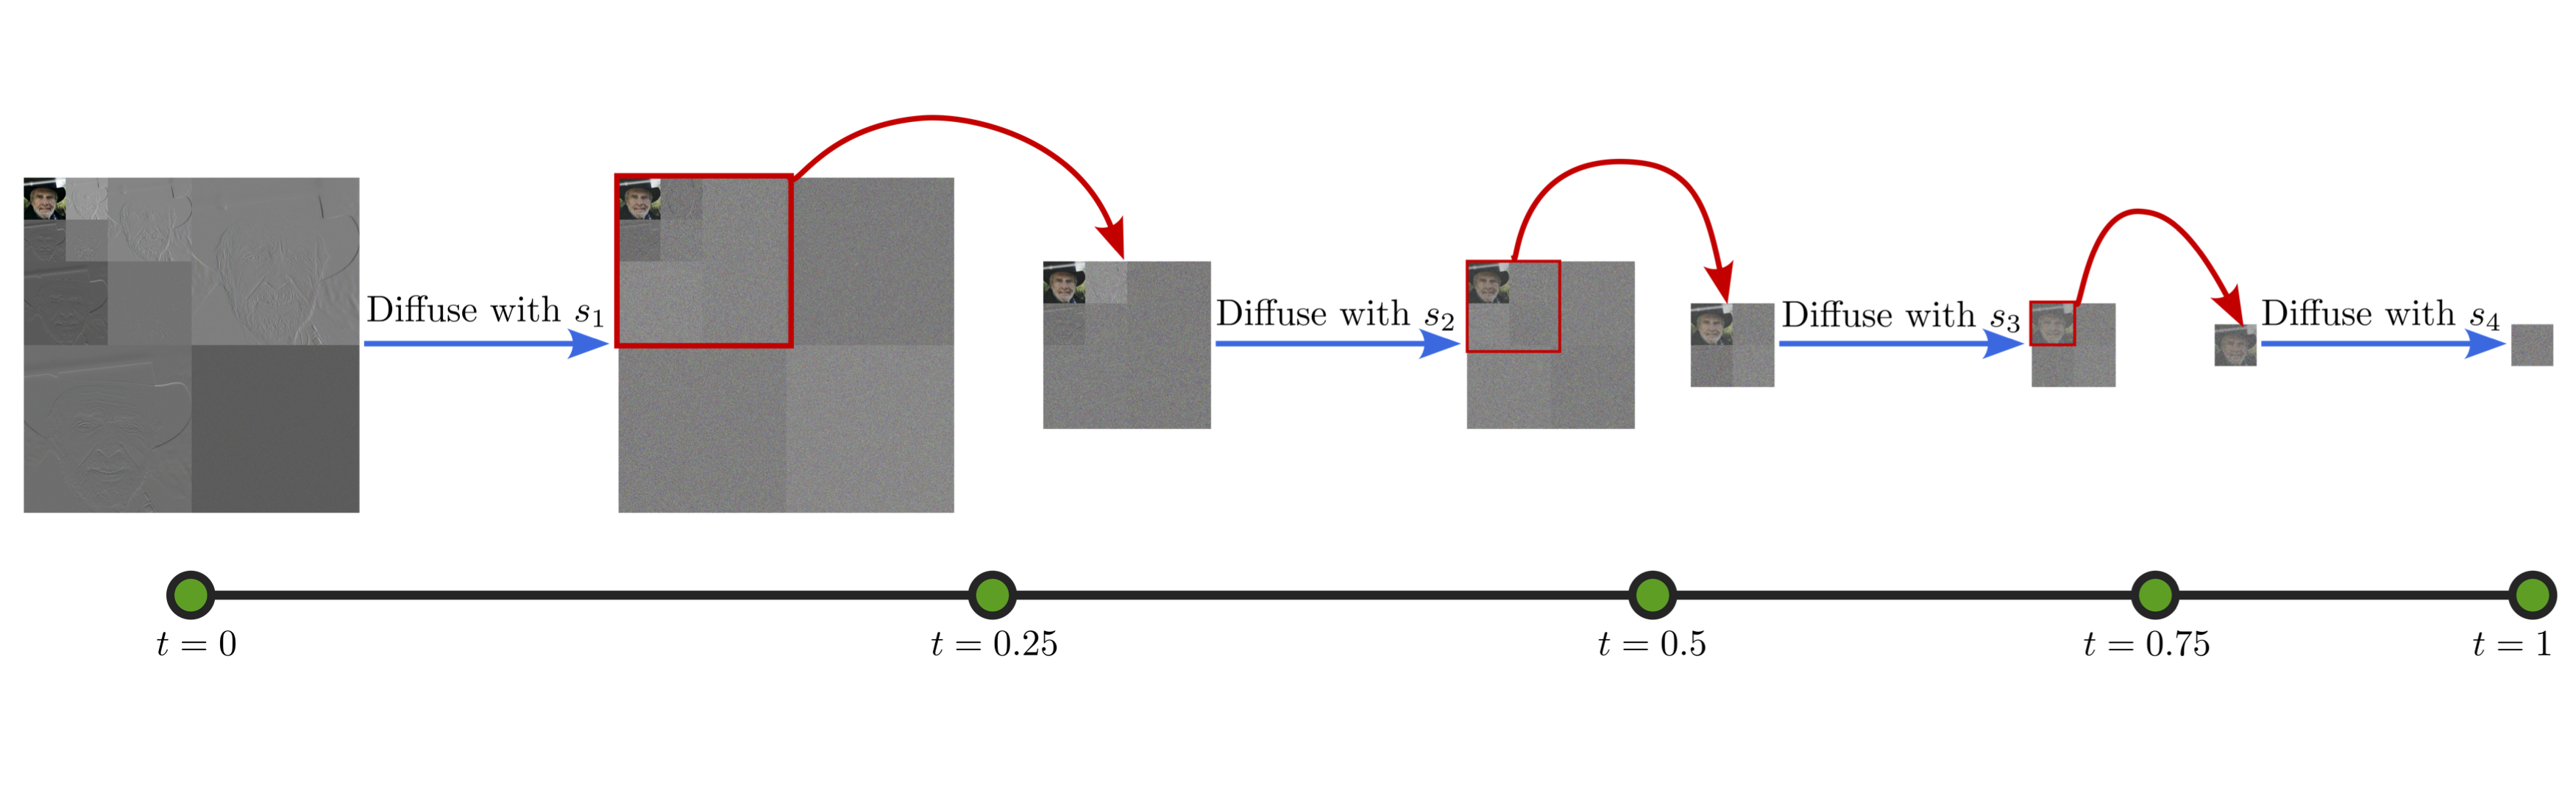
\includegraphics[width=0.9\textwidth]{Outline/figures/non-uniform-diffusion-models/drawing.png}
    \caption{Illustration of a multi-scale diffusion model with three scales. Inspired by multi-scale normalizing flows, this approach diffuses different parts of the image tensor (transformed into multi-level Haar coefficients) at varying speeds. High-frequency detail coefficients diffuse progressively faster, with $d_1$ diffusing faster than $d_2$, $d_2$ faster than $d_3$, and so on, ensuring that all coefficients reach the same (very low) signal-to-noise ratio (SNR) at their respective terminal diffusion times: $t = 0.25, 0.5, 0.75$, and $1.0$, respectively. The low-frequency approximation coefficients $a_3$ diffuse the slowest, completing their diffusion at $t = 1.0$. The multi-scale structure reduces the dimensionality of the diffusing tensor at each scale, enabling faster computation. Separate neural networks $S_1, S_2, S_3, S_4$ approximate the score functions at different intervals, leveraging the reduced dimensionality of the intermediate distributions. This hierarchical design mirrors the structure of multi-scale normalizing flows, improving training and sampling efficiency while maintaining high image generation quality.}
    \label{fig:Multiscale model}
\end{figure}

\begin{figure}[h]
    \begin{center}
    \begin{tabular}{ccc}
        \scriptsize Original image $x$ & \scriptsize  Observation $y$ &  \scriptsize  Sample from $p_\theta(x|y)$  \\

        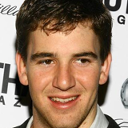
\includegraphics[width=.13\textwidth]{Outline/figures/non-uniform-diffusion-models/797_x.png} &   
        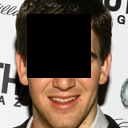
\includegraphics[width=.13\textwidth]{Outline/figures/non-uniform-diffusion-models/797_y.png} &
        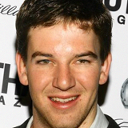
\includegraphics[width=.13\textwidth]{Outline/figures/non-uniform-diffusion-models/797_1.png}  \\

          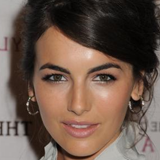
\includegraphics[width=.13\textwidth]{Outline/figures/non-uniform-diffusion-models/x.png} &   
        
\includegraphics[width=.13\textwidth]{Outline/figures/non-uniform-diffusion-models/y.png} &
        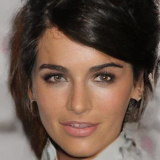
\includegraphics[width=.13\textwidth]{Outline/figures/non-uniform-diffusion-models/DV.png}  \\

        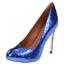
\includegraphics[width=.13\textwidth]{Outline/figures/non-uniform-diffusion-models/189_x.png} &   
        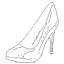
\includegraphics[width=.13\textwidth]{Outline/figures/non-uniform-diffusion-models/189_y.png} &
        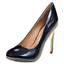
\includegraphics[width=.13\textwidth]{Outline/figures/non-uniform-diffusion-models/189_2.png}  \\
    \end{tabular}
    \end{center}
    \caption{Results from our conditional multi-speed diffusive estimator.}
    \label{fig: teaser}
\end{figure}

In chapter \ref{Chapter:non-uniform-diffusion-models}, we introduce \emph{non-uniform diffusion models}. Unlike standard diffusion approaches that apply the same noise injection schedule to every pixel, non-uniform diffusion models allow different pixels (or groups of pixels) to evolve at varying speeds. This flexibility mirrors the hierarchical approach of multi-scale normalizing flows, where transformations occur at multiple scales, enabling the model to capture image structure more efficiently and produce higher-quality samples in less time. By carefully choosing which parts of the image diffuse faster, non-uniform diffusion opens the door to significantly improved performance, both in terms of image fidelity and computational speed.

We demonstrate that non-uniform diffusion models outperform standard uniform diffusion models by achieving superior FID scores in less training time. Furthermore, these models exhibit remarkable efficiency, sampling up to 4.4 times faster at a resolution of $128 \times 128$, with even greater speed-ups anticipated at higher resolutions. Leveraging the adaptability of non-uniform diffusion, we introduce the Conditional Multi-Speed Diffusive Estimator (CMDE), a novel approach derived from a specific choice of non-uniform diffusion. CMDE unifies existing methods for conditional score estimation and delivers performance on par with the widely adopted conditional denoising estimator.

On the theoretical side, we introduce a principled objective for training non-uniform diffusion models and provide a proof of consistency for the conditional denoising estimator, thereby establishing the reliability of the most widely adopted approach to training conditional diffusion models.

Beyond these theoretical and methodological advances, we conduct a comprehensive empirical evaluation of different approaches to training conditional diffusion methods, comparing their effectiveness across tasks such as super-resolution, inpainting, and edge-to-image translation. Finally, to encourage future research and practical adoption, we release MSDiff, an open-source library dedicated to non-uniform and conditional diffusion models, enabling other researchers and practitioners to easily experiment with and build upon our work.

\subsection*{Originality and Author’s Contributions}

This chapter is adapted from \cite{batzolis2022non_uniform}.  The author’s contributions to this work are as follows:

\begin{itemize}
\item \textbf{Formulation of Ideas}: I came up with the idea of non-uniform diffusion and how to train non-uniform diffusion models. This idea led to multi-scale diffusion and the CMDE estimator which can be used for training conditional diffusion models. Jan Stanczuk noticed that CMDE is an interpolation between CDE and CdiffE.
\item \textbf{Experimental Design}: Myself and Jan Stanczuk had equal contribution in the experimental design.
\item \textbf{Code and Experimental Implementation}: I implemented the experiments presented in the paper. Myself and Jan Stanczuk had equal contribution in the delevopment of the codebase.
\item \textbf{Theory}: The ideas for the proofs of Theorem 1 and 2 were found together. Final technical ideas were completed by Jan Stanczuk. Jan Stanczuk also compiled the proof of Theorem 3.
\item \textbf{Presentation}: The design of the paper was discussed together. Jan Stanczuk led the write up of the paper. I contributed to experimental sections of the write up.
\end{itemize}

This project was conducted under the supervision of Carola-Bibiane Sch\"onlieb and Christian Etmann.

\section{Diffusion Models Encode the Intrinsic Dimension of Data Manifolds}

\begin{figure}[h]
    \centering
    % First subfigure
    \begin{subfigure}[t]{0.45\linewidth}
        \centering
        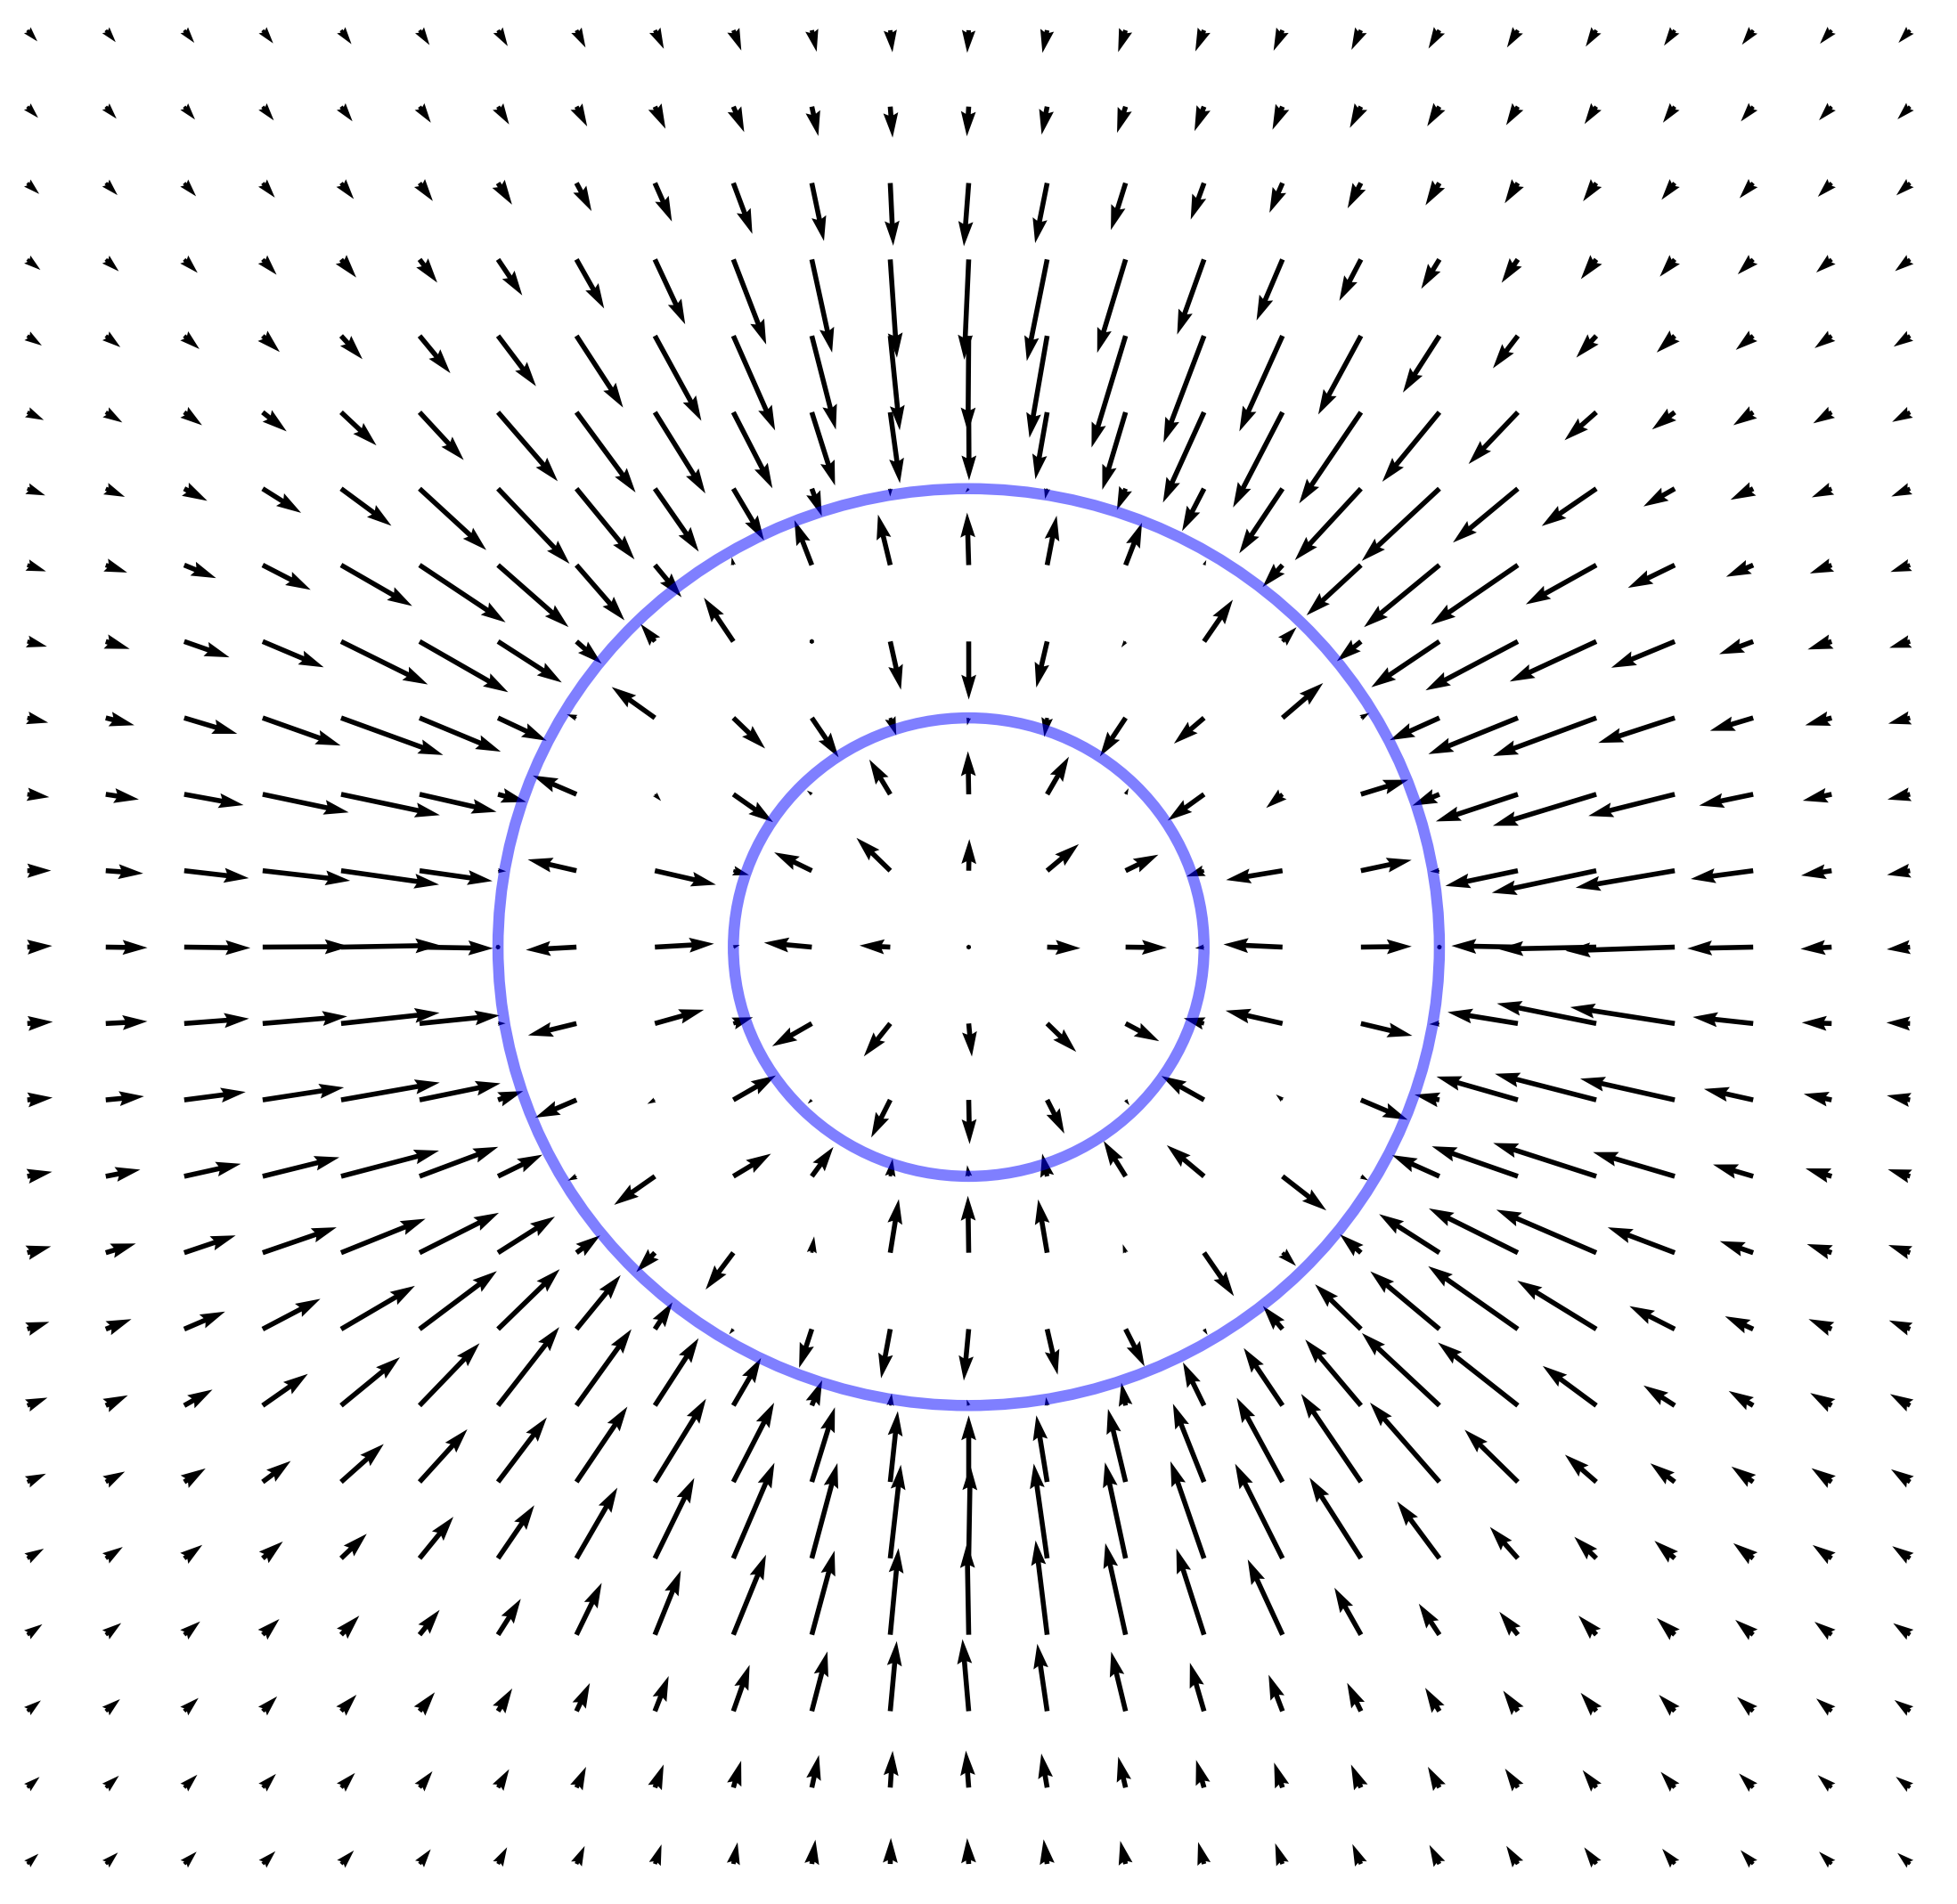
\includegraphics[width=\linewidth]{Outline/figures/id-diff/score_field.png}
        \caption{The data manifold (in blue) and the neural approximation of the score field $\nabla_\textbf{x} \ln p_{t_0}(\textbf{x})$ obtained from a diffusion model. Near the manifold, the score field is perpendicular to the manifold surface.}
        \label{fig:score_field}
    \end{subfigure}
    \hspace{0.05\linewidth} % Space between the figures
    % Second subfigure
    \begin{subfigure}[t]{0.45\linewidth}
        \vspace{-70mm} % Move the figure upwards
        \centering
        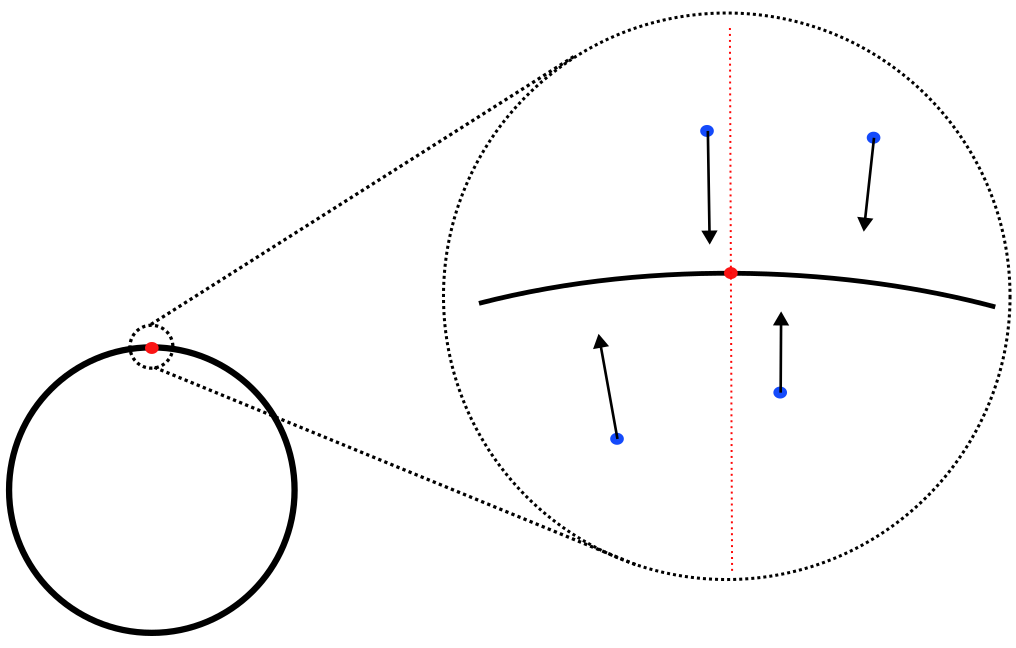
\includegraphics[width=\linewidth]{Outline/figures/id-diff/drawing.png}
        \caption{The red dot shows a point $\textbf{x}_0$ on the data manifold where we wish to estimate the dimension. We sample $K$ blue points $\textbf{x}_t^{(i)}$ in a close neighborhood of the red point and evaluate the score field. The resulting vectors $s_\theta(\textbf{x}_\epsilon^{(i)}, \epsilon)$ point in the normal direction. We put the vectors into a matrix and perform SVD to detect the dimension of the normal space. The dimension of the manifold equals the number of (almost) vanishing singular values.}
        \label{fig:zoom}
    \end{subfigure}
    \caption{(Left) Visualization of the score field near the data manifold. (Right) Visualisation of the estimation of the manifold dimension using the trained diffusion model.}
    \label{fig:score_estimation}
\end{figure}



In chapter \ref{Chapter:intrinsic-dimension}, we provide a mathematical proof
that diffusion models encode data manifolds by
approximating their normal bundles. Based on
this observation we propose a novel method for
extracting the intrinsic dimension of the data manifold from a trained diffusion model. Our insights
are based on the fact that a diffusion model approximates the score function i.e. the gradient
of the log density of a noise-corrupted version of
the target distribution for varying levels of corruption. We prove that as the level of corruption
decreases, the score function points towards the
manifold, as this direction becomes the direction
of maximal likelihood increase. Therefore, at
low noise levels, the diffusion model provides us
with an approximation of the manifold’s normal
bundle, allowing for an estimation of the manifold’s intrinsic dimension. To the best of our
knowledge our method is the first estimator of
intrinsic dimension based on diffusion models
and it outperforms well established estimators in
controlled experiments on both Euclidean and
image data.

\subsection*{Originality and Author’s Contributions}

This chapter is adapted from our published work presented at ICML 2024 on intrinsic dimension estimation with diffusion models \cite{pmlr-v235-stanczuk24a}. The authors' contributions to this work are as follows:

\begin{itemize}
\item \textbf{Formulation of Ideas}: Myself and Jan Stanczuk equally contributed to the formulation of ideas.
\item \textbf{Experimental Design}: Myself and Jan Stanczuk shared equal contributions to the experimental design.
\item \textbf{Code and Experimental Implementation}: Myself and Jan Stanczuk had equal contribution in the developement of the code framework used to run the experiments. I implemented the following experiments: synthetic image manifolds and MNIST dimensionality estimation. Jan Stanczuk implemented the following experiments: k-spheres, line manifold, spaghetti line, comparison with auto-encoder on MNIST, robustness analysis, and all benchmark methods.
\item \textbf{Theory}: Jan Stanczuk derived the theoretical results with help from Teo Deveney.
\item \textbf{Presentation}: Jan Stanczuk and I equally contributed to the write-up, with Teo Deveney contributing to the theoretical sections.
\end{itemize}

This project was conducted under the supervision of Carola-Bibiane Sch\"onlieb.

\section{ScoreVAE: Variational Diffusion Auto-encoder}

\begin{figure}[htbp]
    \centering
    \includegraphics[width=0.8\linewidth]{Outline/figures/scoreVAE/ffhq.png}
    \caption{Comparison of original and reconstructed images on the FFHQ dataset using our ScoreVAE framework. The left panel presents the original images from the FFHQ dataset, while the right panel displays the corresponding reconstructions generated by ScoreVAE. The results highlight the effectiveness of ScoreVAE in capturing intricate details and preserving high fidelity, overcoming the limitations of traditional VAE models.}
    \label{fig:ffhq}
\end{figure}


In chapter \ref{Chapter:ScoreVAE}, we introduce \textbf{ScoreVAE}, a novel approach that advances the Variational Autoencoder (VAE) framework by addressing fundamental limitations of conventional VAEs. Traditional VAEs model the reconstruction distribution $p(\mathbf{x}|\mathbf{z})$ as a Gaussian, which often leads to overly smoothed and blurry reconstructions. This limitation arises because the Gaussian assumption fails to capture the complexity and multimodality of real-world data distributions, making it difficult for the model to accurately represent intricate details and sharp features. ScoreVAE addresses this issue by combining a diffusion-time-dependent encoder and an unconditional diffusion model. By employing Bayes' rule for score functions, we analytically derive a robust and flexible model for reconstruction distribution $p(\mathbf{x}|\mathbf{z})$. Our approach bypasses the unrealistic Gaussian assumption, resulting in significantly improved image reconstruction quality.

The ScoreVAE framework also simplifies the training dynamics by decoupling the training of the diffusion model and the encoder. This decoupling enables the use of powerful pre-trained diffusion models that can be readily updated or swapped without retraining the entire system. By separating the prior (diffusion model) from the encoder, ScoreVAE achieves higher fidelity reconstructions compared to traditional VAEs and diffusion decoders. Our experiments on the CIFAR10 and CelebA datasets demonstrate ScoreVAE’s superiority in producing sharper images and reducing reconstruction error. These results underscore the practical advantages of ScoreVAE in handling complex, high-dimensional data, and highlight its potential for improved representation learning and controllable generative modeling.

\subsection*{Originality and Author’s Contributions}

This chapter is adapted from \cite{batzolis2023variational}. The authors' contributions to this work are as follows:

\begin{itemize}
\item \textbf{Formulation of Ideas}: Myself and Jan Stanczuk contributed equally to the formulation of ideas.
\item \textbf{Experimental Design}: Myself and Jan Stanczuk had equal contributions to the experimental design.
\item \textbf{Code and Experimental Implementation}: I implemented the code for ScoreVAE model (encoder-only, corrector), adaptation of discrete prior models to continuous time framework and the following experiments: reconstructions with score-VAE and Diffusion Decoder. Jan Stanczuk implemented the beta-VAE and code for semantic manipulation.
\item \textbf{Theory}: I suggested the sketch of the proof that entailed connecting the ScoreVAE loss to marginal likelihood \cite{song2021maximum}, and Jan Stanczuk derived the rigorous proof.
\item \textbf{Presentation}: Myself and Jan Stanczuk contributed equally to the final write-up.
\end{itemize}

This project was supervised by Carola-Bibiane Sch\"onlieb.

\section{Score-Based Pullback Riemannian Geometry}

\begin{figure}[h]
    \centering

    % First row: Projections of RAE for three datasets
    \begin{subfigure}[b]{0.32\textwidth}
        \centering
        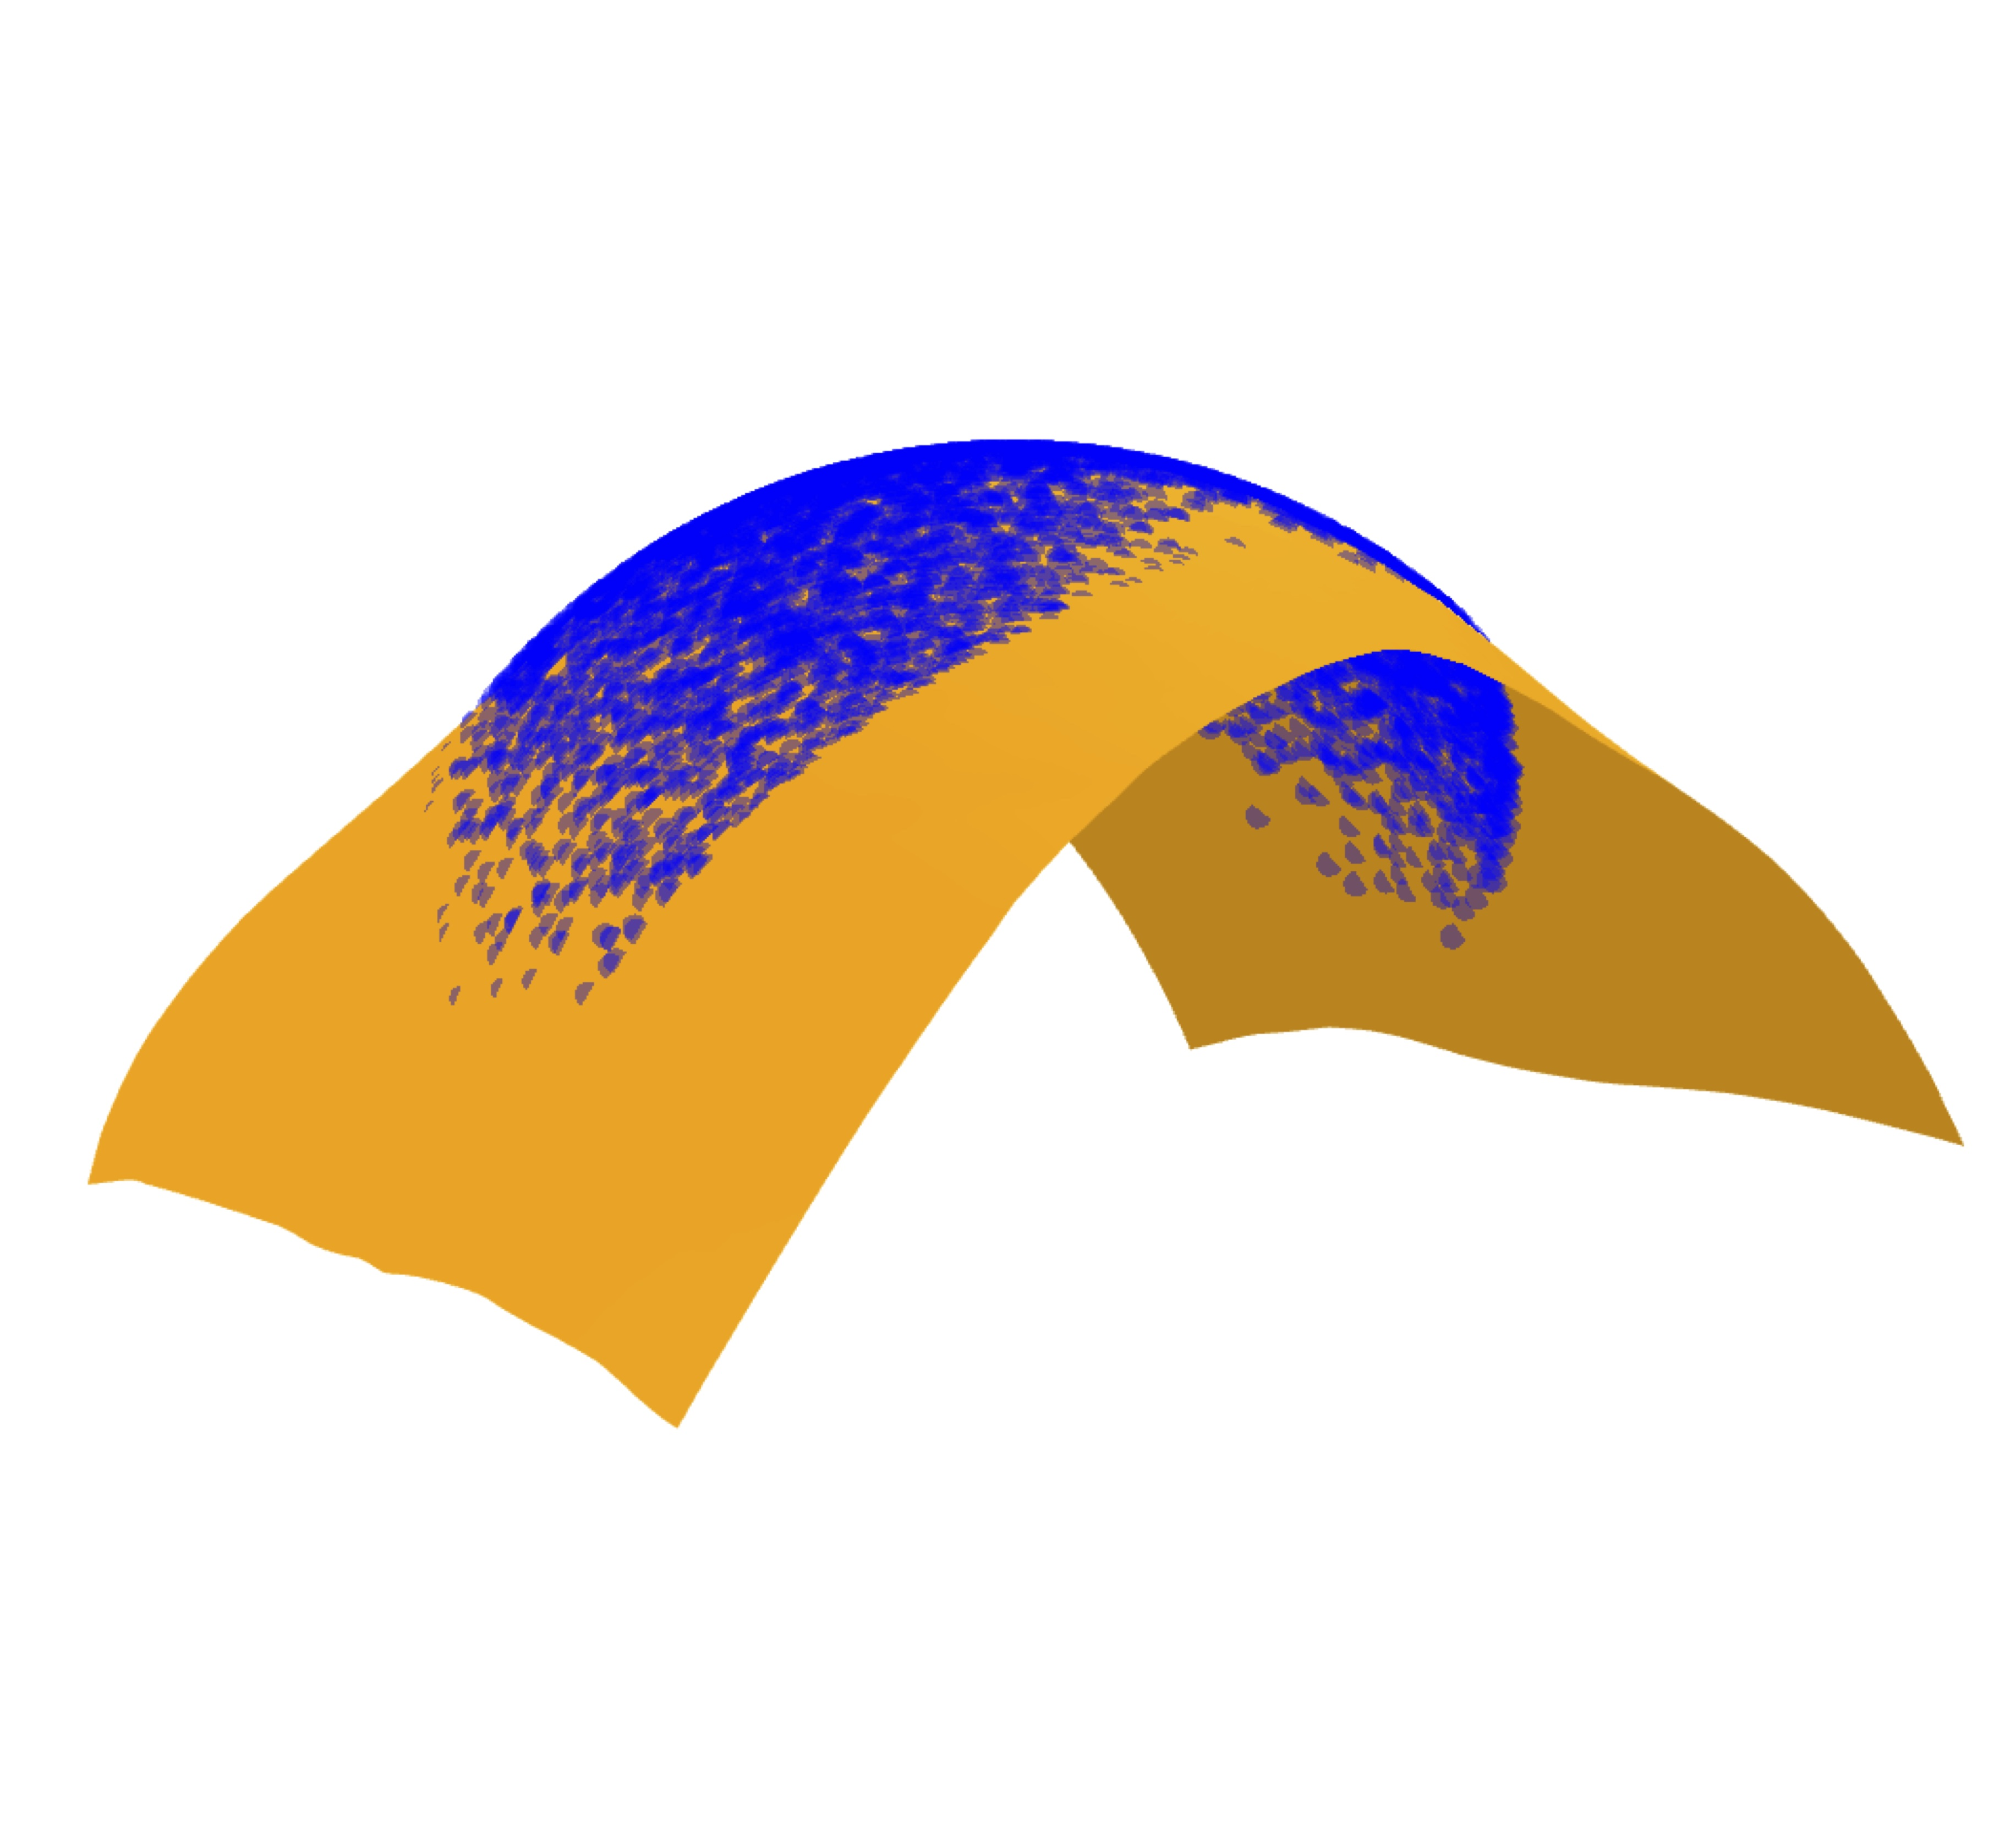
\includegraphics[width=0.7\textwidth]{Outline/figures/score-based-riemannian-geometry/hemisphere.jpg}
        \caption{Hemisphere (2,3)}
    \end{subfigure}
    \hfill
    \begin{subfigure}[b]{0.32\textwidth}
        \centering
        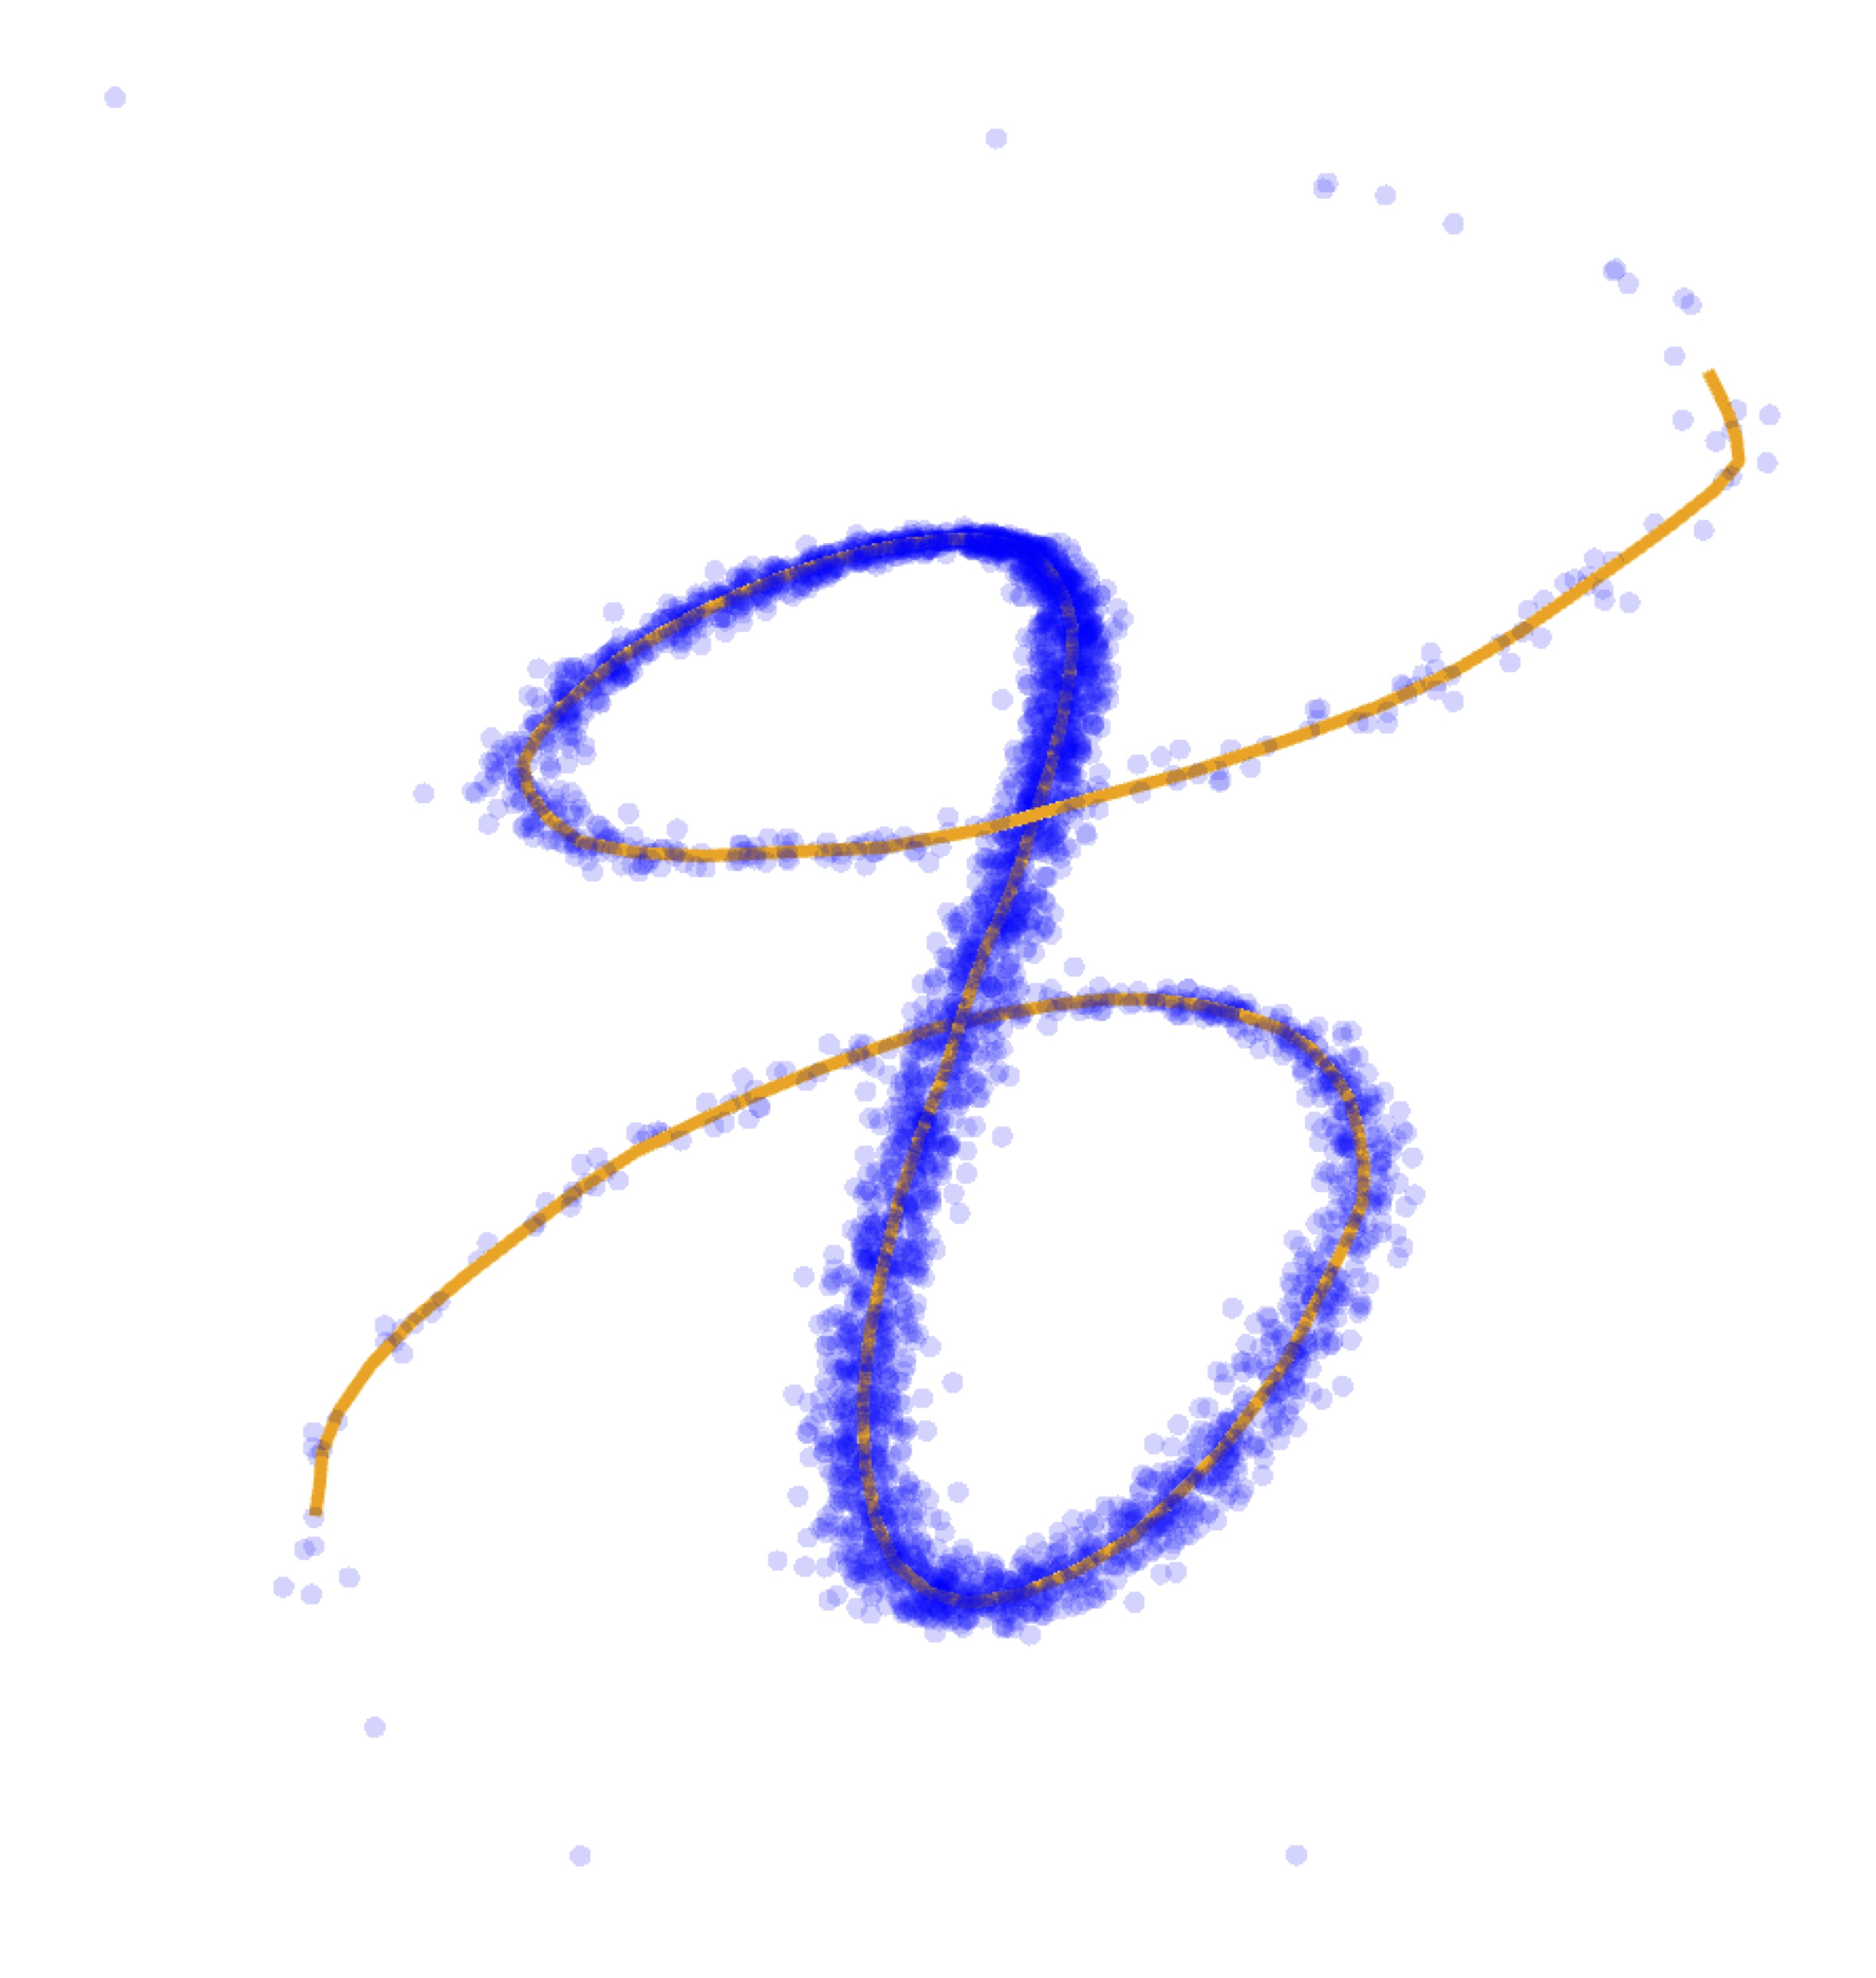
\includegraphics[width=0.7\textwidth]{Outline/figures/score-based-riemannian-geometry/sinusoid_1_3.jpg}
        \caption{Sinusoid (1,3)}
    \end{subfigure}
    \hfill
    \begin{subfigure}[b]{0.32\textwidth}
        \centering
        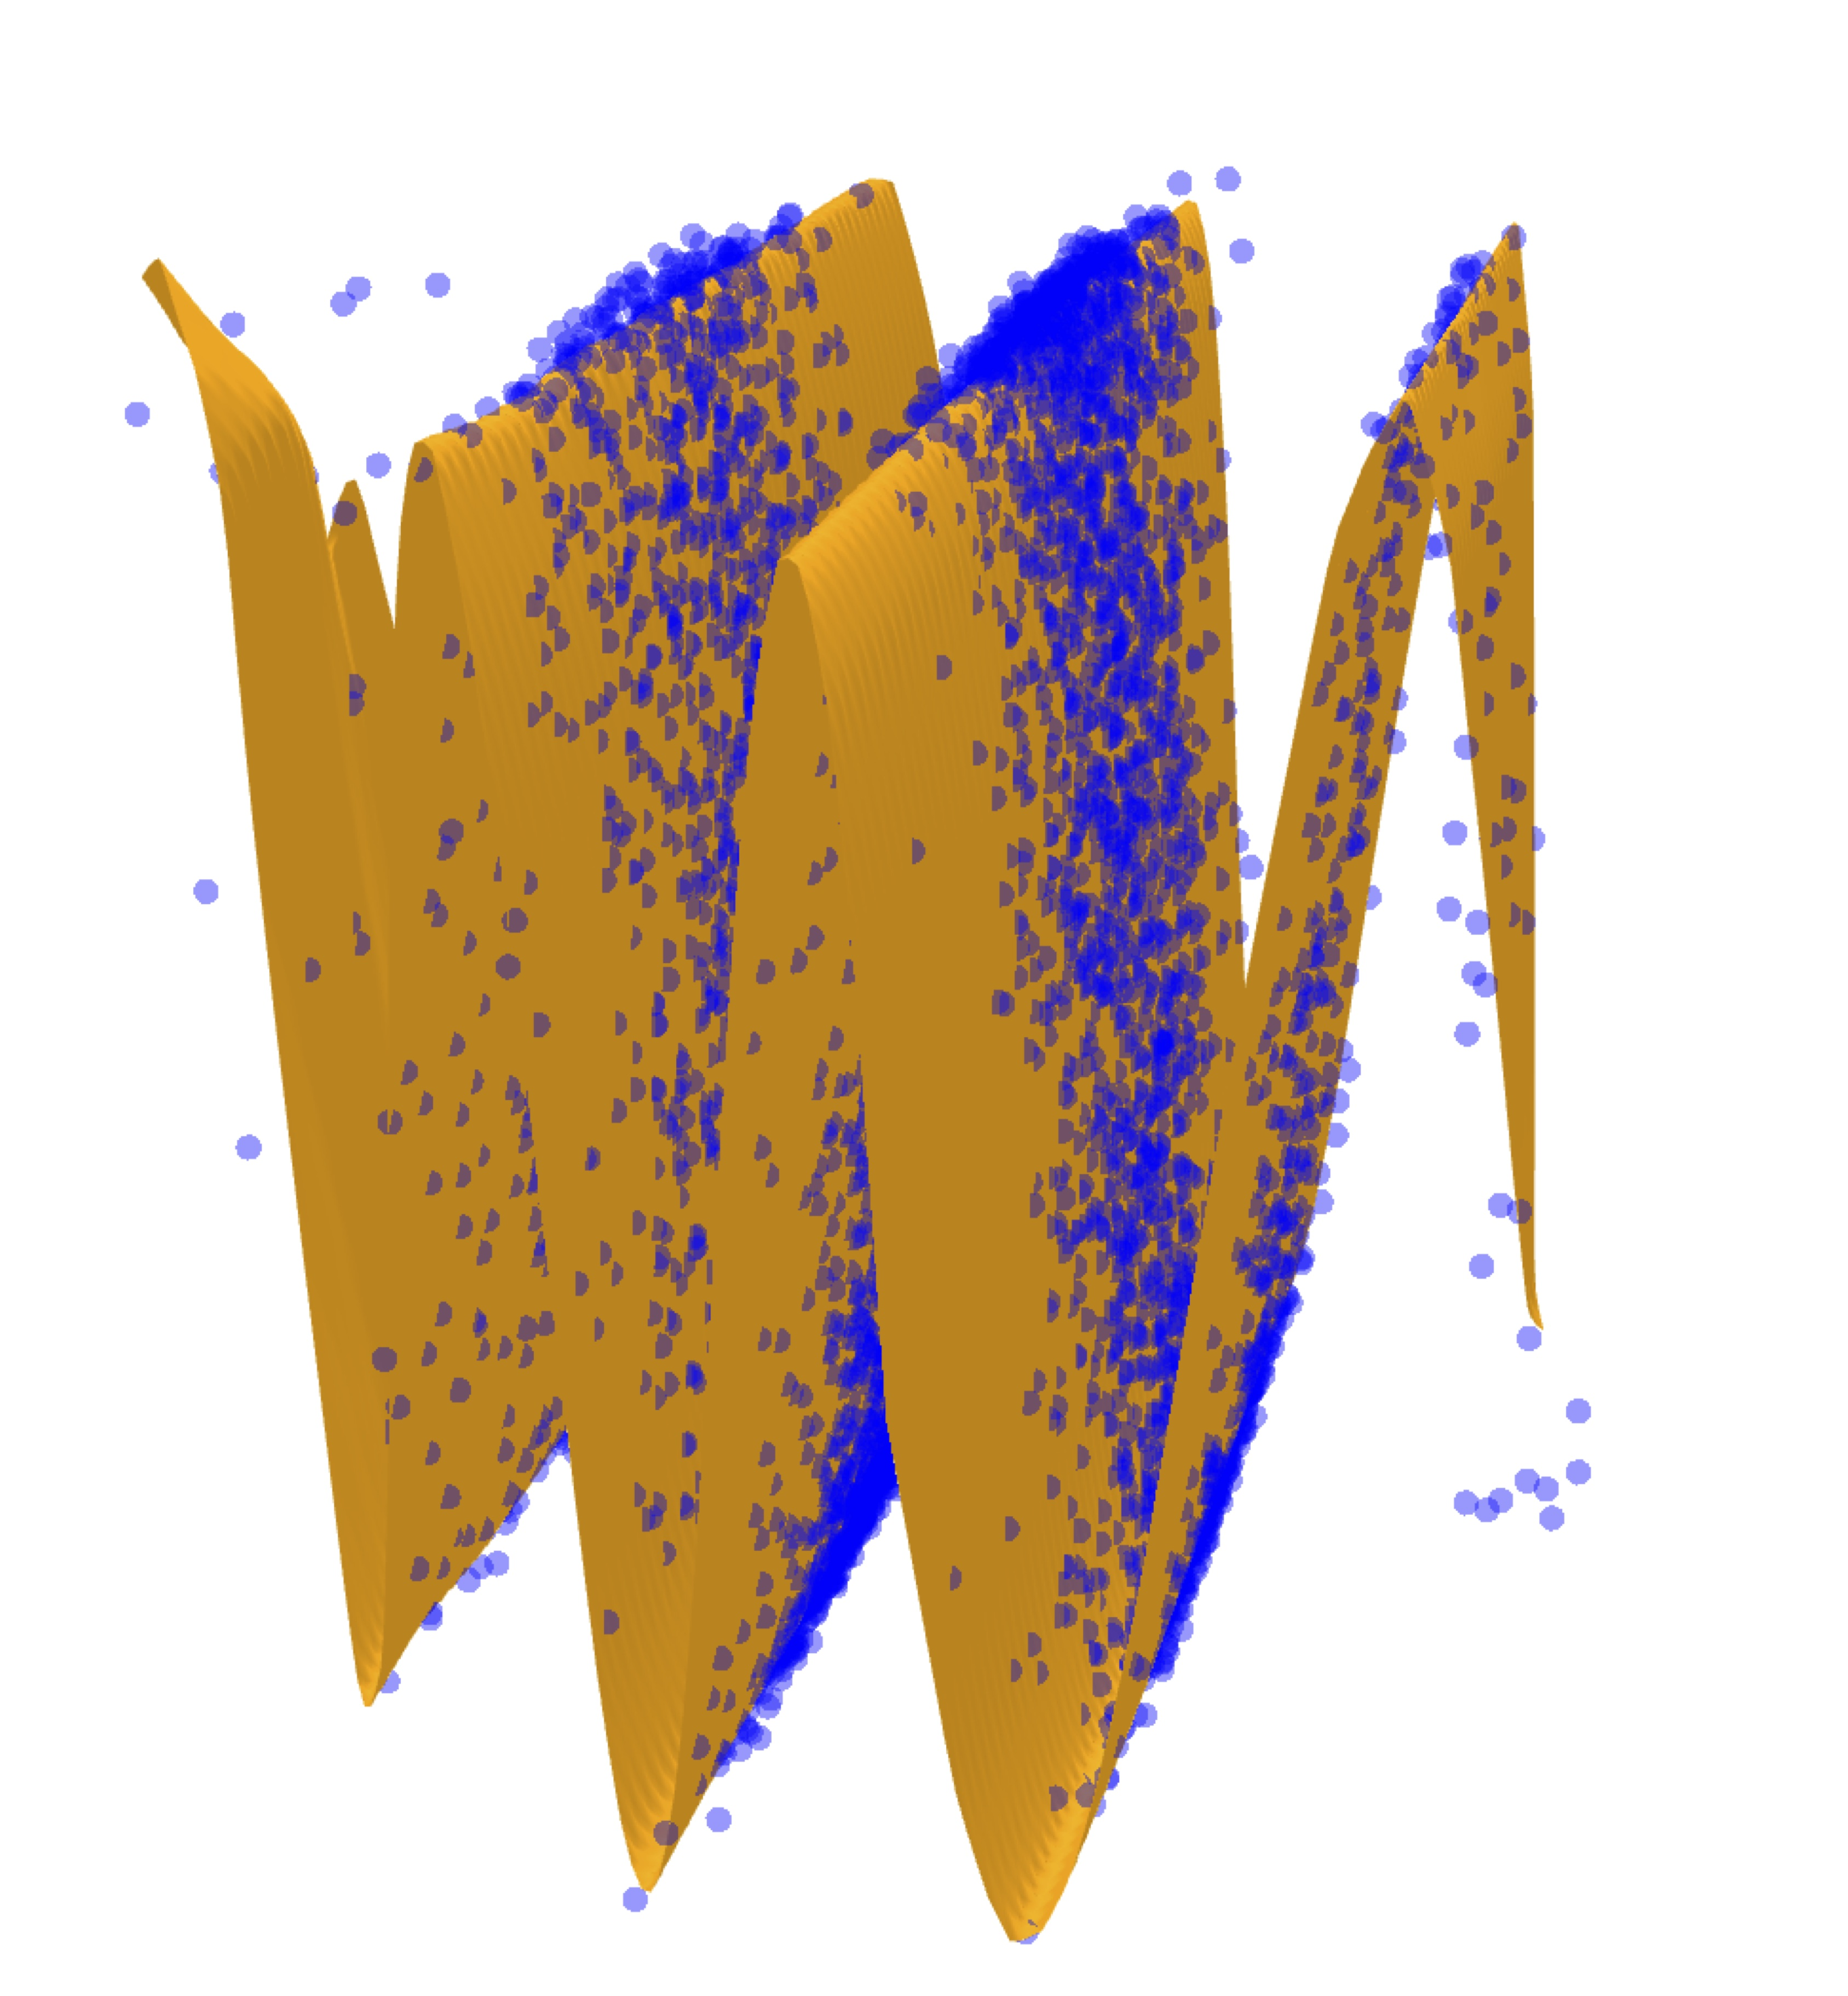
\includegraphics[width=0.7\textwidth]{Outline/figures/score-based-riemannian-geometry/sinusoid_2_3.jpg}
        \caption{Sinusoid (2,3)}
    \end{subfigure}

    \caption{
        Approximate data manifolds learned by the Riemannian autoencoder generated by score-based pullback Riemannian geometry for three datasets. The orange surfaces represent the manifolds learned by the model, while the blue points correspond to the training data. Each manifold provides a convincing low-dimensional representation of the data, isometric to its respective latent space.
    }
    \label{fig:learned_charts}
\end{figure}

In chapter \ref{Chapter:Pullback-riemannian-geometry}, we introduce a score-based pullback Riemannian metric that encodes the intrinsic dimensionality and geometry of data under certain distributional assumptions. We show that this data-driven metric can be constructed in practice by modifying normalizing flows with anisotropic base distribution and isometry regularization. This approach yields a scalable framework for computing manifold maps—such as geodesics, exponential maps, distances, and curvature—in closed form. Building on this metric, we additionally construct a Riemannian Auto-encoder (RAE) that recovers the true manifold dimension, offers a global chart of the manifold, and yields an interpretable latent representation thanks to isometry regularization.

\subsection*{Originality and Author’s Contributions}

This chapter is adapted from \cite{diepeveen2024score}. The authors' contributions to this work are as follows:

\begin{itemize}
\item \textbf{Formulation of Ideas}: Willem Diepeveen proposed the idea of extracting the data manifold's geometry using a score-based pullback metric. He developed the theoretical motivation of using the score-based metric and showed that the constructed metric allows the computation of manifold maps such as geodesics, exponential map, logarithmic map and distance in closed form. Moreover, he showed that the trained normalizing flow used for the construction of the pullback metric is a Riemannian Auto-encoder.

I figured out that the proposed metric can be constructed in practice by adapting the framework of Normalizing flows with base distribution anisotropy and $l_2$ regularisation. Moreover, I discovered the existence of a hessian vector product term that can negatively impact the performance of the Riemannian Auto-encoder if not taken into consideration. 
Including the hessian vector product term in the regularisation allowed us to use non-affine flows reliably which led to the improvement of the scalability and performance of the method.

\item \textbf{Experimental Design}: I led the experimental design, incorporating suggestions from Willem Diepeveen and Zakhar Shumaylov.
\item \textbf{Code and Experimental Implementation}: I implemented the training code and conducted all hyperparameter tuning and experiments. Willem implemented the functionality for constructing the data-driven manifold maps and the Riemannian autoencoder from a trained model.
\item \textbf{Theory}: Willem developed the theoretical results. I contributed by explaining the necessity of Hessian-vector product regularization.
\item \textbf{Presentation}: Zakhar and Willem wrote all sections except for the experimental section, which I authored.
\end{itemize}

This project was conducted under the supervision of Carola-Bibiane Sch\"onlieb.


%!TEX root = ../thesis.tex  % Comment this line for standalone compilation
%*******************************************************************************
%*********************************** First Chapter *****************************
%*******************************************************************************

\chapter{CAFLOW: Conditional Autoregressive Flows}  %Title of the First Chapter

\ifpdf
    \graphicspath{{Chapter1/Figs/Raster/}{Chapter1/Figs/PDF/}{Chapter1/Figs/}}
\else
    \graphicspath{{Chapter1/Figs/Vector/}{Chapter1/Figs/}}
\fi

In this work, we introduce CAFLOW, a new diverse image-to-image translation model that simultaneously leverages the power of autoregressive modeling and the modeling efficiency of conditional normalizing flows. We transform the conditioning image into a sequence of latent encodings using a multi-scale normalizing flow and repeat the process for the conditioned image. We model the conditional distribution of the latent encodings by modeling the autoregressive distributions with an efficient multi-scale normalizing flow, where each conditioning factor affects image synthesis at its respective resolution scale. Our proposed framework performs well on a range of image-to-image translation tasks. It outperforms former designs of conditional flows because of its expressive autoregressive structure.

%********************************** %First Section  **************************************
\section{Introduction}

Generative modeling has emerged as one of the most widely-researched areas in deep learning over the last few years. While generative adversarial networks (GANs) \cite{GANs} produce state-of-the-art results for images \cite{viazovetskyi2020stylegan2}, they do not allow for the estimation of likelihoods. Other types of generative methods, however, admit the explicit evaluation of likelihoods of points under the given model, and thus allow for training as maximum likelihood estimators. Normalizing flows \cite{rezende2015variational} (and their continuous formulation, via NeuralODEs \cite{neuralODEs}) are one such example. These \emph{flow-based} models are diffeomorphic neural networks, which are trained to invertibly transform data into e.g. a normal distribution. This is made possible by a change-of-variables formula, which expresses the likelihood of a data sample in terms of the normal distribution. Samples from the approximated distribution are then generated by passing samples from a normal distribution through the inverse function.

A straightforward extension of likelihood estimators are \emph{conditional} likelihood estimators, which represent the likelihood of a random variable conditioned on another random variable. This is in particular used in autoregressive models and their flow-based variants (\emph{autoregressive flows} \cite{autoregressive_flows}). These types of models explicitly parametrize joint likelihoods via the product rule for probability densities, and can hence be used for creating expressive likelihood estimators, at the cost of more involved computations. This approach is in particular employed by Wavelet Flows \cite{WAVELET-FLOW}, which use a hierarchical multi-scale representation via Wavelet decompositions in order to parametrize expressive conditional likelihood functions for images.

Conditional likelihood estimators are also used for domain transfer and image-to-image translation \cite{Dual-Glow, SRFLOW, ardizzone2019guided, cGLOW} achieving comparable performances to GAN-based models in super-resolution \cite{SRFLOW, HCFLOW}, inpainting \cite{cGLOW} and image-to-image translation \cite{Pumarola2020, Dual-Glow, grover2020alignflow}. In domain transfer, the task is to \emph{transfer} a data point from some \emph{origin} domain (e.g. black-and-white images) to a different \emph{target} domain, e.g. color images in this example. The technique of conditioning lends itself well to domain transfer, as it is possible to condition likelihood functions over the target domain on points from the origin domain, thereby making conditional generation possible. In flow-based models, this has been introduced in the form of conditional flows, which function based on this general principle. The most successful examples of conditional flows are \cite{SRFLOW} and \cite{HCFLOW} which achieved state-of-the-art performance in image super-resolution by adapting conditional flows to the task of image super-resolution. Both methods rely on powerful feature extractors specifically optimised for image super-resolution to extract conditional features from the low resolution image. This makes them not easily applicable to general inverse problem solving.

\medskip

\textbf{Outline of the main contributions}. In this work, we introduce CAFLOW, \emph{conditional autoregressive flow}, which combines the idea of conditional flows with the expressiveness of autoregressive models using hierarchical multi-scale flows for domain transfer. Our goal is to improve the performance of conditional flows on %general inverse problem solving 
general inverse problems in vision.\color{black}

As a first step, we encode the condition and the target images using invertible networks into a hierarchical sequence of $n$ latent spaces. Then, using the chain rule of probability, we decompose the conditional distribution of the latent encodings into $n$ autoregressive component distributions with the aim of modeling each distribution using a conditional normalizing flow. Modeling the theoretical autoregressive components can be computationally very expensive. For this reason, we used a small set of assumptions that allowed us to design a computationally efficient multiscale normalizing flow at a small modeling flexibility cost. By carefully designing such a flow based on weak assumptions on the mutual dependencies of the latent encodings, our model allows for exchange of information between latent spaces of different dimension. In particular, our designed architecture is able to capture correlations between different scales, improving on the expressivity of other conditional flow-based models used for domain transfer tasks. The training of the $n$ conditional flows can be parallelized, however, the sampling process is sequential and could become computationally expensive if the number of scales is large. However, in practice, the choice of the invertible networks that map the images to latent encodings does not allow the number of scales $n$ to be large, which makes the sampling time of CAFLOW much smaller than that of pure autoregressive models and slightly greater than that of standard conditional flows.

Our modeling choices are corroborated by strong experimental evidence. Using an ablation study, we confirmed experimentally that the autoregressive model outperforms the non-autoregressive model. Furthermore, we demonstrate that our model outperforms standard designs of conditional flows on classical image-to-image translation tasks such as image super-resolution, image colorization and image inpainting. In particular, we show that on these tasks CAFLOW outperforms former designs of conditional flows and GAN-based models thanks to its expressive autoregressive structure.

Concurrently to our work, Liang et al. \cite{HCFLOW} introduced autoregressive conditioning in the latent space, which yielded improved results compared to their earlier work \cite{SRFLOW}. 
However, they make the following restrictive modelling assumption: the low resolution image is part of the target latent space.  This makes their method not applicable to general inverse problems in vision. 

As far as inverse problems on other modalities are considered, our method can be suitably modified to address inverse problems on structured data where there is an underlying hierarchical decomposition of the signal. It is true that our method would not be easily applied in unstructured data such as categorical or tabular data. However, the same applies to all other conditional normalizing flow methods that use a multiscale structure.
\color{black}

\medskip

\textbf{Organization of the paper.} The paper is organized as follows.
In Section \ref{ch1:sec:background}, we provide the necessary theoretical background on unconditional and conditional normalizing flows. In Section \ref{ch1:sec:Caflow}, we describe our CAFLOW method discussing the modeling assumptions and deriving a formula for estimating the log-likelihood of the unknown conditional probability. In Section \ref{ch1:sec:numerics}, we present the quantitative and qualitative results of our experiments. Finally, in Sections \ref{ch1:sec:conclusions} we discuss the limitations of our work and we draw our conclusions. 

\section{Background}\label{ch1:sec:background}

\subsection{Notations}

Random variables will be denoted by capital letters, e.g. $X$, $Y$, while their associated probability will be indicated by $P(X)$, $P(Y)$ and their distributions by $p_X$ and $p_Y$. 
We use calligraphic capital letters, e.g. $\mathcal{X}, \mathcal{Y}$, to denote the sample space of the random variables $X$, $Y$ and small bold letters $\x$, $\y$ for the samples. Finally, given two random variables $X$ and $Y$ we will consider the conditional probability of $Y$ given $X$ and we denote it by $P(Y|X)$. Its density will be indicated by $p_{Y|X}$. We remark that throughout the paper we will always implicitly assume that the considered probabilities admit a density.

\subsection{Normalizing flows}\label{ch1:subsec:normalizing}

Given a random variable $Y$ defined on $\mathcal{Y}$ with an unknown distribution $p_Y$, the main idea of flow-based generative modeling is to approximate $p_Y$ with a learned function $p^\theta_Y$, which is parametrized by an invertible neural network $G^\theta$ mapping from a latent space $\mathcal{Z}$ to $\mathcal{Y}$. 
Choosing $P(Z)$ to be a probability associated to the random variable $Z$ and $p_Z$ its distribution on $\mathcal{Z}$, we define the function $p^\theta_Y$ as the distribution of the push-forward measure of $P_Z$ by the map $G^\theta$.
By the change-of-variables formula for probability distributions, $p^\theta_Y$ is easily computed as
\begin{align*}
p^\theta_Y(\y) = p_Z(F^\theta(\y)) \left| \det \left(\frac{d F^\theta(\y)}{d\y} \right)\right|,
\end{align*}
where $F^\theta$ is the inverse of $G^\theta$.
Thanks to the formula above it is then possible to match $p^\theta_Y$ to $p_Y$ by miminizing the negative log-likelihood of $p^\theta_Y$, defined as
\begin{align*}
- \log p^\theta_Y(\y) = -  \log(p_Z(F^\theta(\y))) -  \log\left| \det \left(\frac{d F^\theta(\y)}{d\y} \right)\right|.
\end{align*}
In practice, the transformation $G^\theta$ is a composition of learnable invertible transformations $G_{1}, ..., G_{n}$ such that $G_i : \mathcal{Z}_{i} \rightarrow \mathcal{Z}_{i+1}$ (where $\mathcal{Z}_1 = \mathcal{Z}$ and $\mathcal{Z}_{n+1} = \mathcal{Y}$) for intermediate latent spaces $\mathcal{Z}_i$ and
\begin{equation}
    \y = G_{n}(G_{n-1}(...G_{1}(\z)))=G^{\theta}(\z)\,, \quad  \z= F_1(F_{2}(...F_n(\y)))=F^{\theta}(\y),
\end{equation}
where $F_i = (G_i)^{-1}$ for every $i$ and thus $F^\theta = (G^\theta)^{-1}$ (Note that we are assuming implicitly that each $G_i$ and $F_i$ depends on $\theta$, but we drop the superscript $\theta$ for notational convenience). This model is called a normalizing flow.
In this case, using the properties of the Jacobian for composition of invertible transformations the log-likelihood of $p^\theta_Y$ can be computed as 
\begin{equation}\label{ch1:ch1:eq:loglike}
\log(p^\theta_Y(\y) ) = \log(p_Z(F^\theta(\y))) + \sum_{i=1}^{n}  \log\left| \det \left(\frac{d{F_i}(\z_{i+1})}{d\z_{i+1}} \right)\right|,
\end{equation}
where $\z_{n+1} = \y$.


In order to estimate $\log(p^\theta_Y(\y) )$ the transformations $G_i$ need to be designed to have a computable inverse $F_i$ and a tractable Jacobian determinant. 
%We next describe typical choices for the transformations $g_i$ introduced in \cite{Nice2014, GLOW} and then commonly used in most of the normalizing flow architectures. We will refer to them in the next sections where we describe our method.
We next present typical choices for the transformations $G_i$. We describe each method by presenting the forward transform $G_i$, the inverse transform $F_i$ and the  log-determinant of the Jacobian. The calculation of the Jacobian determinant is used in the calculation of the log-likelihood in \eqref{ch1:ch1:eq:loglike}.
\color{black}

\medskip

\textbf{Affine coupling layer}. Affine coupling layers \cite{Nice2014} capture complex dependencies of the activations in an invertible and computationally efficient way.

\smallskip

\textit{\underline{Forward Function}}:

A given a tensor \(\z\) is partitioned into two parts: \(\z_1\) and \(\z_2\). The tensor \(\z_2\) remains unchanged and is used in the transformation of \(\z_1\). A nonlinear mapping, represented by NN (typically a shallow convolutional neural network), processes \(\z_2\) producing two outputs of the same dimension as \(\z_1\): \(\boldsymbol{u}\) and \(\boldsymbol{t}\). The exponential of \(\boldsymbol{u}\) is used as the scale and $\boldsymbol{t}$ as the bias of the affine transformation of \(\z_1\). The steps are the following:
\begin{align*}
\z_1, \z_2 &= \text{split}(\z) \\
(\boldsymbol{u},\boldsymbol{t}) &= NN(\z_2) \\
\s &= \exp(\boldsymbol{u}) \\
\y_1 &= \s \odot \z_1 + \boldsymbol{t} \\
\y_2 &= \z_2.
\end{align*}
The final tensors \(\y_1\) and \(\y_2\) merge to produce the output tensor \(\y\).

\smallskip

\textit{\underline{Inverse Function}}:
\begin{align*}
\y_1, \y_2 &= \text{split}(\y) \\
(\boldsymbol{u},\textbf{t}) &= NN(\y_2) \\
\s &= \exp(\boldsymbol{u}) \\
\z_1 &= \frac{(\y_1 - \boldsymbol{t})}{\s} \\
\z_2 &= \y_2.
\end{align*}
Both \(\z_1\) and \(\z_2\) merge to produce the reversed tensor \(\z\).

\smallskip

\textit{\underline{Log-Determinant of the Jacobian}}: The log-determinant of the Jacobian can be computed as:
\[\sum_{i=1}^{d}(\log |\s_i|)
\]where the sum is over all the elements of the tensor $\s$.

\smallskip

\textbf{Invertible \(1 \times 1\) Convolution}.
In the Affine coupling layer, the partitioning of the tensor \(\textbf{z}\) is static, implying that stacking multiple Affine coupling layers still leaves part of the tensor unchanged. This limits the range of inverse functions the model can represent. Addressing this limitation, Kingma et al. \cite{GLOW} introduced the invertible \(1 \times 1\) convolution layer. By blending information across the channel dimension prior to the Affine coupling layer, the invertible \(1 \times 1\) enhances the model's capacity to represent inverse functions of increased complexity.

\smallskip

\textit{\underline{Forward Function}}:
\[
\forall i,j : y_{i,j} = Wz_{i,j},
\]
where:
\begin{itemize}
    \item \(W\) is a weight matrix of size $c \times c$ %shape \([c \times c]\).
    \item \(z_{i,j}\) and \(y_{i,j}\) are spatial indices into tensors \(\z\) and \(\y\), respectively, both of size  $h \times w \times c$.   
    %having the shape \([h \times w \times c]\).
\end{itemize}

\textit{\underline{Inverse Function}}:
\[
\forall i,j : z_{i,j} = W^{-1}y_{i,j}.
\]

\textit{\underline{Log-Determinant of the Jacobian}}:
\[h \cdot w \cdot \log | \det(W)|\]

The computational cost of computing the log-determinant of the Jacobian can be improved from \( O(c^3) \) to \( O(c) \) if $W$ is parametrized in its LU decomposition as follows:

\[ W = PL(U + \text{diag}(\textbf{r})), \] 
where
\begin{itemize} \item \( P \) is a permutation matrix that remains fixed, \item \( L \) is a lower triangular matrix with ones on the diagonal, \item \( U \) is an upper triangular matrix with zeros on the diagonal, \item \( \textbf{r} \) is a vector. \end{itemize}

Here, $P$, $L$, $U$ and \( \textbf{r} \) are initialized by sampling a random rotation matrix $W$ and then computing the values of $P$, $L$, $U$ and \( \textbf{r} \) that correspond to the LU decomposition of $W$. The matrix $P$ remains fixed, while $L$, $U$ and \( \textbf{r} \) are learnable. By parametrizing $W$ in its LU decomposition, the computational complexity is reduced from \( O(c^3) \) to \( O(c) \), because $\log | \det(W)| = \sum_{i=1}^{c}(\log |r_i|)$, where $(r_1,...,r_c)$ are the elements of the vector $r$.

\smallskip

\textbf{Actnorm}. Actnorm, presented in [12], is a modification of the conventional batch normalization [9]. It is tailored to handle stability challenges in training deep models, especially in scenarios where memory constraints mandate a very small batch size per processing unit. Rather than depending on batch statistics, Actnorm executes an affine transformation on activations using a learnable scale and bias parameter per channel. Each channel undergoes unique scaling and biasing. The initial values of the parameters depend on the data, ensuring that the post-actnorm activations per channel have zero mean and unit variance. After this initialization, these parameters are considered trainable and evolve independently of the input data.

\smallskip

\textit{\underline{Forward Function}}:
\[
\forall i,j : y_{i,j} = s \odot z_{i,j} + b,
\]
where:
\begin{itemize}
    \item \(z_{i,j}\) and \(y_{i,j}\) are spatial indices into tensors \(\z\) and \(\y\), both of which are of size $h \times w \times c$.
    %shape \([h \times w \times c]\).
    \item \(s\) and \(b\) are scale and bias parameters, respectively.
\end{itemize}

\textit{\underline{Inverse Function}}:
\[
\forall i,j : z_{i,j} = \frac{(y_{i,j} - b)}{s}.
\]

\textit{\underline{Log-Determinant of the Jacobian}}: The log-determinant of the Jacobian can be computed as:
\[
h \cdot w \cdot \sum_{i=1}^{d}(\log |\s_i|).
\]

These layers are the building blocks of normalizing flows. A typical normalizing flow architecture consists of sequential blocks where each block contains Actnorm layer, an invertible 1x1 convolution layer, and an affine coupling layer in that order. More details about how these layers are utilised to form the normalizing flow architecture are provided in \ref{ch1:unconditional-architecture}.

\subsection{Conditional Normalizing Flows}

The normalizing flow approach can be adapted to model conditional densities of complicated target distributions. Precisely, given two random variables $X$ and $Y$, the conditional distribution $p_{Y|X}$ is parametrized using a transformation $G^\theta : \mathcal{Z} \times \mathcal{X} \rightarrow \mathcal{Y}$ such that $G^\theta(\cdot, \x) : \mathcal{Z} \rightarrow \mathcal{Y}$ is invertible for every condition $\x$. Choosing $P(Z)$ to be a probability associated to the random variable $Z$ defined on $\mathcal{Z}$ and $p_Z$ its distribution on $\mathcal{Z}$, we denote by $p^\theta_{Y|X}$ the distribution of the probability obtained by applying the push-forward by the map $ \z \mapsto G^\theta(\z, \x)$ to $P(Z)$. By the change-of-variables formula for probability distributions the conditional log-likelihood of $p^\theta_{Y|X}$ can be then computed as 
\begin{align}\label{ch1:eq:cond}
\log(p^\theta_{Y|X}(\y|\x)) = \log(p_{Z}(F^\theta(\y,\x)))   +  \log\left| \det \left(\frac{\partial F^{\theta}(\y,\x)}{dy} \right)\right|,
\end{align}
where $F^\theta(\cdot, \x)$ is the inverse of $G^\theta(\cdot, \x)$ for every condition $\x$.
Consequently, a generative model for $p_{Y|X}$ can be trained by minimizing the negative log-likelihood of the parameters $\theta$ using the formula in \eqref{ch1:eq:cond}. The sampling procedure works similarly to standard normalizing flows. We generate a sample $\y \sim p^\theta_{Y|X}(\cdot, \x)$ by sampling a latent $\z\sim p_Z$ and passing it through $G^\theta(\cdot, \x)$, yielding $\y=G^\theta(\z, \x)$. Similarly to traditional normalizing flows the map $G^\theta$ is modeled through a composition of learnable invertible conditional transformations. We describe next the specific layers used in conditional normalizing flow architectures.

\medskip

\textbf{Conditional affine coupling layer}. As a variant of the affine coupling layer, the conditional affine coupling layer integrates an external condition, allowing for conditional modelling. The scale and bias are computed via parametrized functions that consider not only the split activation \(\z_2\), but also the external condition \(\x\). 

\smallskip



\textit{\underline{Forward Function}}:
A given tensor \(\z\) is equally divided into two fixed parts: \(\z_1\) and \(\z_2\). 

Similarly to the unconditional case, a nonlinear mapping represented by $NN$ processes \(\z_2\) and the external condition \(\x\) producing two outputs of the same dimension as \(\z_1\): \(\boldsymbol{u}\) and \(\boldsymbol{t}\). The exponential of \(\boldsymbol{u}\) is used as the scale and $\boldsymbol{t}$ as the bias of the affine transformation of \(\z_1\). The steps are the following:


\begin{align*}
\z_1, \z_2 &= \text{split}(\z) \\
(\boldsymbol{u},\boldsymbol{t}) &= NN(\z_2, \boldsymbol{x}) \\
\s &= \exp(\boldsymbol{u}) \\
\y_1 &= \textbf{s} \odot \z_1 + \boldsymbol{t} \\
\y_2 &= \z_2.
\end{align*}
The resulting tensors, \(\y_1\) and \(\y_2\), are combined to generate the output tensor \(\y\).

\smallskip

\textit{\underline{Inverse Function}}: Reversing the forward function and accounting for the condition \(\x\), we get:
\begin{align*}
\y_1, \y_2 &= \text{split}(\y) \\
(\boldsymbol{u},\boldsymbol{t}) &= NN(\y_2, \boldsymbol{x}) \\
\s &= \exp(\boldsymbol{u}) \\
\z_1 &= \frac{(\y_1 - \boldsymbol{t})}{\boldsymbol{s}} \\
\z_2 &= \y_2.
\end{align*}
Both \(\z_1\) and \(\z_2\) merge to yield the original tensor \(\z\).


\smallskip

\textit{\underline{Log-Determinant of the Jacobian}}: The log-determinant of the Jacobian can be computed as:
\[\sum_{i=1}^{d}(\log |\s_i|).\]

\textbf{Affine Injector}. The Affine Injector layer, introduced in \cite{SRFLOW}, enhances the capability of normalizing flows in transferring information from the conditioning data. Unlike the conditional Affine coupling layer, which influences only a subset of the intermediate activation \(\z\), the Affine Injector impacts all channels and spatial locations of the activation, thereby enabling more comprehensive data flow from the condition to the main branch of the flow. Here, the "main branch of the flow" denotes the series of transformations that process the data tensor and its latent intermediate activations. The scale and bias tensors are parametrized functions of only the condition \(\x\).

\smallskip

\textit{\underline{Forward Function}}:
Given the external condition \(\x\), the nonlinear mapping represented by \(NN\) processes \(\x\) to produce two outputs of the same dimension as \(\z\): \(\boldsymbol{u}\) and \(\boldsymbol{t}\). The exponential of \(\boldsymbol{u}\) is used as the scale and \(\boldsymbol{t}\) as the bias for the affine transformation of \(\z\). The steps are the following:

\begin{align*}
(\boldsymbol{u}, \boldsymbol{t}) &= NN(\boldsymbol{x}) \\
\s &= \exp(\boldsymbol{u}) \\
\y &= \boldsymbol{s} \odot \z + \boldsymbol{t}.
\end{align*}

\smallskip

\textit{\underline{Inverse Function}}:
Reversing the forward function and accounting for the condition \(\x\), we get:
\begin{align*}
(\boldsymbol{u}, \boldsymbol{t}) &= NN(\boldsymbol{x}) \\
\s &= \exp(\boldsymbol{u}) \\
\z &= \frac{\y - \boldsymbol{t}}{\s}.
\end{align*}

\smallskip

\textit{\underline{Log-Determinant of the Jacobian}}:
The log-determinant of the Jacobian can be computed as:
\[\sum_{i=1}^{d}(\log |\s_i|).\]

As empirically demonstrated by Lugmayr et al. \cite{SRFLOW}, the integration of the Affine Injector augments the modeling capacity of the conditional normalizing flow.

\subsection{Conditioning in the Normalizing Flow latent space}
An alternative way for conditional generation using normalizing flows is proposed in \cite{Dual-Glow} in a model named Dual-Glow. The authors couple two multi-scale normalizing flows modeled with a GLOW architecture that interact at different scales. %Their main goal is to synthesize the PET scan conditioned on the MRI scan, but the same architecture has proven to be useful for other standard image-to-image translation tasks.
In particular, denoting by $Y$ and $W$\footnote{In this section, $W$ denotes a random variable, distinct from its previous use as a weight matrix. The notation for the weight matrix will not be used further in this article.} the random variables modeling the distribution of conditioning images and of conditioned images (respectively), they estimate the conditional probability $P(W|Y)$ using two multi-scale normalizing flows which convert images $Y$ and $W$ into sequences of hierarchical latent random variables $[D_{n-1}, ..., D_0]$ and $ [L_{n-1}, ..., L_0]$, respectively, as shown in schematically in Figure \ref{ch1:fig:dependencies}. 
Then, they model the distribution of the latent random variables $ [L_{n-1}, ..., L_0]$ given the latent random variables $[D_{n-1}, ..., D_0]$ by making the assumption that information is exchanged only between latent spaces of the same scale, that is \begin{align}\label{ch1:eq:Dual-Glowdep}
P(L_{n-1}, ..., L_0|D_{n-1}, ..., D_0)  = \prod_{i=0}^{n-1}P(L_{i}|D_{i}).
\end{align}
The final step is the modelling of the each conditional distribution  $P(L_{i}|D_{i})$. They make the assumption that the conditional probability $P(L_{i}|D_{i})$ is a multidimensional Gaussian distribution, whose mean $\mu_i^{\theta}$ and covariance $\Sigma_i^{\theta}$ are parametrised functions of $D_{i}$. In particular, its density is parametrized by the functions $p_{L_{i}|D_{i}}^\theta$ given by
\begin{align}\label{ch1:eq:Dual-Glowdep}
p^\theta_{L_{i}|D_{i}}(\boldsymbol{\ell}_i, \boldsymbol{d}_i)  = \mathcal{N}(\boldsymbol{\ell}_i; \mu_i^{\theta}(\boldsymbol{d}_{i}), \Sigma_i^{\theta}(\boldsymbol{d}_i)) \quad i = 0,\ldots, n-1.
\end{align}


The decomposition of conditioning and conditioned images into sequences of hierarchical latent spaces that exchange information at different scales is a natural approach to conditional probability estimation. Indeed, it offers the possibility to prescribe the rate of information exchange between different scales and to monitor the information flow in a more accurate way. In the next section we will discuss how our method is taking advantage of such flexibility, by decomposing the conditional distribution of the latent encodings and decodings in its autoregressive components.

\section{Method}\label{ch1:sec:Caflow}
The aim of our CAFLOW model is to perform image-to-image translation tasks by learning the conditional distribution $P(W|Y)$ where $W$ and $Y$ are random variables that model given image distributions.
Following a similar architecture to \cite{Dual-Glow} we use two multi-scale normalizing flows $R^\theta$ and $T^\theta$ to convert images $Y$ and $W$ into two sequences of $n$ hierarchical latent variables defined on latent space of decreasing dimension: \(R^\theta(Y)=\tilde{D}_n\), where \(\tilde{D}_n:=[D_{n-1}, ..., D_0]\) and \(T^\theta(W)=\tilde{L}_n\), where \(\tilde{L}_n := [L_{n-1}, ..., L_0]\). Then we design an autoregressive model based on conditional normalizing flows to learn the conditional distribution $P(\tilde{L}_n| \tilde{D}_n)$.

\subsection{Modeling assumptions}\label{ch1:subsec:modass}

\begin{figure}[t]
\centering
   \begin{subfigure}{0.31\textwidth}
		\includegraphics[width=\textwidth]{Chapter1/figures/fulldependencies.png}
	\end{subfigure}%
	\quad
\begin{subfigure}{0.31\textwidth}
	\includegraphics[width=\textwidth]{Chapter1/figures/Dual-Glowdependencies.png} 
\end{subfigure}%
\quad 
\begin{subfigure}{0.31\textwidth}
	\includegraphics[width=\textwidth]{Chapter1/figures/oursdependencies.png}
	\end{subfigure}
\caption{From left to right: ideal dependencies in the $i^{th}$ autoregressive component. Dual-Glow modeling assumption \cite{Dual-Glow}; information is exchanged only between latent spaces having the same dimension. Our modeling assumption; we retain the dependencies between $L_i$ and the latent spaces of lower dimension.}	\label{ch1:fig:dependencies}
\end{figure}

The conditional distribution $P(\tilde{L}_n| \tilde{D}_n)$ is factorized using the chain rule of probability into $n$ autoregressive component distributions as shown in \eqref{ch1:conditional-distribution-autoregressive-factorization}:
\begin{equation}\label{ch1:conditional-distribution-autoregressive-factorization}
    P(\tilde{L}_n| \tilde{D}_n) = \prod_{i=0}^{n-1}P(L_i|\tilde{L}_{i},D_{n-1},...,D_0)
\end{equation}
with the notational convention that $\tilde{L}_{0}=\emptyset$ and $\tilde L_{i} = [L_{i-1}, \ldots, L_0]$ for every $i$. The dependencies of the $i^{th}$ component distribution are shown graphically in the left diagram of Figure \ref{ch1:fig:dependencies}. Modeling those $n$ autoregressive distributions can be unnecessarily computationally expensive. For this reason, we assume that 
\begin{equation}\label{ch1:eq:factorization}
    P(\tilde{L}_n| \tilde{D}_n)= \prod_{i=0}^{n-1}P(L_i|\tilde{L}_{i},\tilde D_{i+1}),
\end{equation}
where $\tilde D_{i+1} = [D_{i}, \ldots, D_0]$. In particular, we retain the dependencies between $L_{i}$ and all $L$ and $D$ latent variables of level $i$ and below, which effectively means that we are pruning only the dependencies between  $L_{i}$ and $D_{i+1},...,D_{n-1}$. We advocate that this is a valid assumption, because the encoded information in the split variables of the multi-scale flow typically ranges from local noise patterns and image details to higher-level information as we move from the early split variables to the final split variables.  The hierarchical representation in multi-scale normalizing flows is attributed to the interplay of depth of computation and the information bottleneck. We refer the reader to Appendix \ref{ch1:Hierarchical-Representation-in-Multi-Scale-Normalizing-Flows} for a more detailed discussion. \\ \color{black}
We remark that our modeling assumption is weaker than the one implicitly used in \cite{Dual-Glow} described in \eqref{ch1:eq:Dual-Glowdep} (see Figure \ref{ch1:fig:dependencies}). Precisely we allow information to be exchanged between latent spaces of different dimension. As we will demonstrate in the experiments our choice allows for more expressive architectures able to capture correlations between different scales.
We represent schematically in Figure \ref{ch1:fig:dependencies} the difference between the theoretical latent space dependencies, the one assumed in \cite{Dual-Glow} and our modeling choice. 
Under this modeling assumption, our goal is to estimate the conditional distributions $P(L_i|\tilde{L}_{i},\tilde D_{i+1})$ for every $i$ and then recover 
$P(\tilde{L}_n| \tilde{D}_n)$ using \eqref{ch1:eq:factorization}.

\subsection{Modeling the autoregressive components using conditional normalizing flows}\label{ch1:Autoregressive-conditional-flow-components}
%
%We propose to estimate each autoregressive component $P(L_i|\tilde{L}_{i},\tilde D_{i+1})$ using a multi-scale conditional normalizing flow architecture.

Modeling the autoregressive components $P(L_i|\tilde{L}_{i},\tilde D_{i+1})$ in a computationally efficient way is challenging because of the dependence on the multiple latent factors of different dimension that encode different semantic content. We propose to estimate each autoregressive component $P(L_i|\tilde{L}_{i},\tilde D_{i+1})$ with a novel multiscale normalizing flow architecture that efficiently incorporates the latent conditions. \color{black}For every $i=0, \ldots, n-1$ we define a sequence of latent variables $\tilde Z_{i+1} := [Z_{i}^{i},...,Z_0^{i}]$ defined on latent spaces of decreasing dimension $\tilde{\mathcal{Z}}_{i+1} := [\mathcal{Z}_{i}^{i},...,\mathcal{Z}_0^{i}]$ and a parametrized transformation

\begin{align*}
    G^\theta_i : \tilde{\mathcal{Z}}_{i+1} \times  \tilde{\mathcal{D}}_{i+1} \times  \tilde{\mathcal{L}}_{i} \rightarrow \mathcal{L}_{i}.
    \end{align*}
    The transformations $G^\theta_i$ are constructed by assembling multi-scale transformations $(g_j^i)_{j=0}^i$ (implicitly depending on the parameter $\theta$) defined as follows:
    \begin{align*}
    &g_0^i : \mathcal{Z}_0^i \times \mathcal{D}_0 \times \mathcal{L}_0 \rightarrow \mathcal{Z}_{0}^{\prime i} \\   
     &  g_{j}^{i}:\mathcal{Z}_{j-1}^{\prime i}\times \mathcal{Z}_{j}^{i} \times \mathcal{D}_{j} \times  \mathcal{L}_{j} \rightarrow \mathcal{Z}_{j}^{\prime i}\, \quad \text{for} \quad j=1,...,i-1\\
    &g_{i}^{i}: \mathcal{Z}_{i-1}^{\prime i}\times \mathcal{Z}_{i}^i \times \mathcal{D}_{i} \rightarrow     \mathcal{L}_{i}
\end{align*}

where $\mathcal{Z}_{i-1}^{\prime i}, \ldots, \mathcal{Z}_0^{\prime i} $ are intermediate latent spaces of decreasing dimension, $g_j^i$ is invertible as a function from $\mathcal{Z}_{j-1}^{\prime i} \times \mathcal{Z}_{j}^i$ to $\mathcal{Z}_{j}^{\prime i}$ and $g_0^i$  is invertible as function from $\mathcal{Z}_0^i$ to $\mathcal{Z}_{0}^{\prime i}$.
The transformation $G^\theta_i$ is then obtained by composing the functions  $g_{j}^{i}$ in the following way. Given the conditioning variables $(\de_j)_{j=0}^i \in \tilde{\mathcal{D}}_{i+1}$ and $(\el_j)_{j=0}^{i-1} \in \tilde{\mathcal{L}}_{i}$, a latent variable $\z_0 \in \mathcal{Z}_0^i$ is transformed to $\z_0' \in \mathcal{Z}_0^{\prime i}$ by function $g^i_0(\cdot ; \de_0, \el_0)$. 
Then $\z_0'$ and $\z_1$ are concatenated and inserted to $g^i_1(\cdot;\de_1, \el_1)$ which outputs $\z_1' \in \mathcal{Z}_1^{\prime i}$. This process continues as implied up until the $i^{th}$ level whose output is $\el_i = g_i^i(\z_{i-1}', \z_i; \de_i) \in \mathcal{L}_{i}$. A schematic description of $G^\theta_i$ is presented in the right diagram of Figure \ref{ch1:fig:high_level_design_conditional}. 

Denote by $f_{j}^{i}$ (implicitly depending on the parameter $\theta$) the inverse of $g_{j}^{i}$ for fixed conditioning variables in $\mathcal{D}_j$ and $\mathcal{L}_j$
\begin{align*}
&f_0^i : \mathcal{Z}_0^{\prime i} \times \mathcal{D}_0 \times \mathcal{L}_0 \rightarrow \mathcal{Z}_0^i \\   
 &  f_{j}^{i}:  \mathcal{Z}_{j}^{\prime i} \times \mathcal{D}_{j} \times  \mathcal{L}_{j} \rightarrow \mathcal{Z}_{j-1}^{\prime i}\times  \mathcal{Z}_{j}^i\, \quad \text{for} \quad j=1,...,i-1\\
&f_{i}^{i}:    \mathcal{L}_{i} \times \mathcal{D}_{i} \rightarrow  \mathcal{Z}_{i-1}^{\prime i}\times \mathcal{Z}_{i}^i
\end{align*}
and by $F_i^\theta$ the inverse of $G_i^\theta$ as a function from $\tilde{\mathcal{Z}}_{i+1}$ to $\mathcal{L}_i$ obtained by composing the functions $f^i_j$ for $j = 0, \ldots, i$.
We model each $f_{j}^{i}$ by adopting the conditional flow design of \cite{SRFLOW}. More specifically, we initially use the same squeeze layer, which is followed by two transition steps and $K$ conditional flow steps. Each transition step consists of an actnorm layer followed by $1\times1$ invertible convolution layer. Each conditional flow step consists of an actnorm layer followed by $1\times1$ invertible convolution, which is followed by an affine injector and an affine coupling layer. We use from 8 to 16 conditional flow steps depending on the difficulty of the image translation task.

\smallskip

\textbf{A discussion on sharing weights strategies.} It is worth noting that the multi-scale transformations, denoted as \(g_j^i\), for all transformations \(G_i^{\theta}\) where \(i \geq j+1\), share the same architecture and function – integrating information from conditions \(D_j\) and \(L_j\). This hints at the potential of utilizing a singular subflow, \(g_j^{j+1}\), for every \(G_i^{\theta}\) with \(i \geq j+1\). Such a strategy could decrease the computational burden and introduce an inductive bias. Yet, it is crucial to recognize that this approach assumes the only distinctive subflow in each \(G_i^{\theta}\) flow is \(g_i^i\). All the deeper subflows, represented by \(g_k^i\) where \(k<i\), are shared between \(G_i^{\theta}\) and other \(G_j^{\theta}\) flows. This results in a modeling constraint, narrowing the space of functions the architecture can represent. Our preliminary tests confirmed this limitation; the performance using this approach significantly lags behind the more generalized model presented in this paper.

\begin{figure}[t]
    \centering
    \begin{subfigure}{0.45\textwidth}
        \includegraphics[width=\textwidth]{Chapter1/figures/dual_glow.pdf}
    \end{subfigure}%
    \qquad 
    \begin{subfigure}{0.47\textwidth}
            \includegraphics[width=\textwidth]{Chapter1/figures/high_level_design_conditional_modified.pdf}
    \end{subfigure}
    \caption{Left: unconditional normalizing flow architecture used to encode conditioning and conditioned images, denoted by $Y_n = Y$ and $W_n = W$ respectively, into a sequence of hierarchical latent variables. Right: design of the conditional transformation $G_{i}^\theta$ that models the $i^{th}$ autoregressive component. The index of the flow $i$ is omitted in both the transformed latent variable $Z_j$ and the intermediate latent variables $Z_j^{\prime}$ for simplicity.}
           \label{ch1:fig:high_level_design_conditional}
\end{figure}

\subsection{Maximum log-likelihood estimation and training}
Here we use the constructed transformations $G_i^\theta : \tilde{\mathcal{Z}}_{i+1} \times  \tilde{\mathcal{D}}_{i+1} \times  \tilde{\mathcal{L}}_{i} \rightarrow \mathcal{L}_{i}$ to parametrize each autoregressive component $P(L_i|\tilde{L}_{i},\tilde D_{i+1})$ and, together with the unconditional normalizing flows $R^{\theta} := R^\theta_n \circ \ldots \circ R^\theta_1$ and $T^{\theta}:= T^\theta_n \circ \ldots \circ T^\theta_1$, use them to estimate $P(W|Y)$. To model $ P(\tilde{L}_n| \tilde{D}_n)$ through its autoregressive componenents as in \eqref{ch1:conditional-distribution-autoregressive-factorization}, we define 
the operator $G^\theta : \tilde{\mathcal{Z}}_{1} \times \ldots \times \tilde{\mathcal{Z}}_{n} \times  \tilde{\mathcal{D}}_{n}  \rightarrow \tilde{\mathcal{L}_{n}}$ as the concatenation of the operators $G^\theta_i$ defined in the previous section, i.e. 
\begin{align}\label{ch1:eq:G}
    G^\theta = [G^\theta_0, \ldots, G^\theta_{n-1}].
\end{align}
where $G^\theta_i$ is computed inductively using $G^\theta_j$ for $j<i$ as in the autoregressive factorization \eqref{ch1:conditional-distribution-autoregressive-factorization}.
Then we consider the map $H^\theta :  \tilde{\mathcal{Z}}_{1} \times \ldots \times \tilde{\mathcal{Z}}_{n} \times \mathcal{Y}\rightarrow \mathcal{W}$ defined as  $H^\theta(\tilde \z_1, \ldots, \tilde \z_n, \y):= (T^\theta)^{-1}( G^\theta(\tilde \z_1, \ldots, \tilde \z_n ; R^\theta(\y)))$ and we denote by $p^\theta_{W|Y}$ the distribution of the pushforward measure
\begin{align}
    H^\theta_\#(\cdot, \y) P([\tilde Z_{1}, \ldots, \tilde Z_{n}]).
\end{align}
We minimize the negative log-likelihood of $p^\theta_{W|Y}$ to obtain an estimate of $P(W|Y)$.
With this aim, for every latent variable $Z_j^i$ in $\tilde Z_j$ we choose as prior a multivariate normal distribution, whose density we denote by $\mathcal{N}(\cdot; \textbf{0}, \textbf{I})$.
In the next theorem we provide an explicit formula for the logarithm of $p^\theta_{W|Y}$ expressed in terms of $R^\theta_i$, $T^\theta_i$ and $f^i_j$.

\begin{proposition}
    The logarithm of $p^\theta_{W|Y}$ can be computed as
    \begin{align}
    \log p^\theta_{W|Y}(\boldsymbol{w} | \y)   & = \sum_{i=1}^{n}\log{\Bigg|{\rm det}\frac{\partial T_i^{\theta}(\boldsymbol{w}_{n-i+1})}{\partial \boldsymbol{w}_{n-i+1}}\Bigg|} \nonumber \\ 
    & + \sum_{i=1}^{n-1} \sum^{i-1}_{j=0} \left[\log \mathcal{N}(\z_j^i;\textbf{0},\textbf{I})+\log \Bigg|{\rm det}\left(\frac{\partial f^i_{j}(\z_j^{\prime i};\el_j,\de_{j})}{\partial \z_j^{\prime i}}\right)\Bigg|\right] \nonumber\\
    & + \sum_{i=0}^{n-1}  \left[\log \mathcal{N}(\z_i^i;\textbf{0},\textbf{I})+\log \Bigg|{\rm det}\left(\frac{\partial f^i_{i}(\el_{i};\de_{i})}{\partial \el_{i}}\right)\Bigg|\right]\label{ch1:eq:obj}
    \end{align} 
    
    where the normal distributions are computed in the latent variables $\z_j^i = f_j^i(\z_j^{\prime i}, \boldsymbol{d}_j,\boldsymbol{l}_j)$ and $\z_i^i = f_i^i( \boldsymbol{d}_i,\boldsymbol{l}_i)$. Moreover, each intermediate latent variable $\z_j^{\prime i}$ is defined recursively by the application of the previous $f_j^i$ (see Figure \ref{ch1:fig:high_level_design_conditional}) and ${\de}_{i} \in \mathcal{D}_{i}$ implicitly depend on $\y \in Y$ through the normalizing flow $R^\theta$. 
    
\end{proposition}

\begin{proof}
    First we express the logarithm of $p^\theta_{W|Y}$ in terms of $p^\theta_{\tilde{L}_n|\tilde{D}_n}$, where  $p^\theta_{\tilde{L}_n|\tilde{D}_n}$ is the distribution induced by the map $G^\theta$ defined in \eqref{ch1:eq:G}. We obtain
    \begin{equation}\label{ch1:eq:equationone}
    \begin{aligned}
         \log p^\theta_{W|Y}(\boldsymbol{w} | \y)=& \log \Big|\text{det}\Bigg(\frac{\partial T^\theta(\boldsymbol{w})}{\partial \boldsymbol{w}}\Bigg)\Big| + \log{p^\theta_{\tilde{L}_n|\tilde{D}_n}(\tilde{\el}_n|\widetilde{\de}_n)} \\ 
        =& \sum_{i=1}^{n}\log{\Bigg|\text{det}\frac{\partial T_i^{\theta}(\boldsymbol{w}_{n-i+1})}{\partial \boldsymbol{w}_{n-i+1}}\Bigg|}+ \log{\prod_{i=0}^{n-1}p^\theta_{L_i|\tilde{L}_{i},\tilde D_{i+1}}(\el_i|\tilde{\el}_{i},\widetilde \de_{i+1})} \\
        =& \sum_{i=1}^{n}\log{\Bigg|\text{det}\frac{\partial T_i^{\theta}(\boldsymbol{w}_{n-i+1})}{\partial \boldsymbol{w}_{n-i+1}}\Bigg|}+ \sum_{i=0}^{n-1}\log{p_{L_i|\tilde{L}_{i},\tilde D_{i+1}}^\theta(\el_i|\tilde{\el}_{i},\widetilde \de_{i+1})}.
    \end{aligned}
    \end{equation}
    
    The justification for the first line can be found in  \cite[Section 3]{Dual-Glow}. In the second line we use the chain rule for distribution and we factorize the conditional distribution using the dependency assumptions of our model. Now observe that
    
    \begin{equation}\label{ch1:eq:equationtwo}
    \begin{aligned}
        \sum_{i=0}^{n-1}\log{p_{L_i|\tilde{L}_{i},\tilde D_{i+1}}^\theta(\el_i|\tilde{\el}_{i},\widetilde \de_{i+1})}
         =& \sum_{i=0}^{n-1}\log{p_{\tilde{Z}_{i+1}}(F_i^{\theta}(\el_i;\tilde{\el}_{i},\widetilde \de_{i+1}))}\\
         &  +\log{\Bigg|\text{det}\frac{\partial F_i^{\theta}(\el_i;\tilde{\el}_{i},\widetilde \de_{i+1})}{\partial \el_i}\Bigg|} \\
        =& \sum_{i=1}^{n-1} \sum^{i-1}_{j=0} \Bigg[\log \mathcal{N}(\z_j^i;\textbf{0},\textbf{I})\\
        &  +\log \Bigg|\text{det}\left(\frac{\partial f^i_{j}(\z_j^{\prime i};\el_j,\de_{j})}{\partial \z_j^{\prime i}}\right)\Bigg|\Bigg] \\
    & + \sum_{i=0}^{n-1}  \left[\log \mathcal{N}(\z_i^i;\textbf{0},\textbf{I})+\log \Bigg|\text{det}\left(\frac{\partial f^i_{i}(\el_{i};\de_{i})}{\partial \el_{i}}\right)\Bigg|\right],
    \end{aligned}
    \end{equation}
    where the normal distributions are computed in the latent variables $\z_j^i = f_j^i(\z_j^{\prime i}, \boldsymbol{d}_j,\boldsymbol{l}_j)$ and $\z_i^i = f_i^i( \boldsymbol{d}_i,\boldsymbol{l}_i)$.
    The first line of \eqref{ch1:eq:equationtwo} is obtained by using the change-of-variables formula. In the second line we use the chain rule for the composition of functions using the definition of $F_{i}^{\theta}$ in \ref{ch1:Autoregressive-conditional-flow-components} and the assumption that the latent variables $Z_i^i,Z_{i-1}^i, ..., Z_0^i$ which comprise $\tilde{Z}_{i+1}$ are i.i.d. with distribution $\mathcal{N}(\textbf{0},\textbf{I})$. The sum is then broken into two sums, because the $f_i^i$ functions are conditioned only on $\de_i$ by definition. Therefore, combining \eqref{ch1:eq:equationone} and \eqref{ch1:eq:equationtwo} we obtain
    
    \begin{align}
    \log p^\theta_{W|Y}(\boldsymbol{w} | \y)   & = \sum_{i=1}^{n}\log{\Bigg|\text{det}\frac{\partial T_i^{\theta}(\boldsymbol{w}_{n-i+1})}{\partial \boldsymbol{w}_{n-i+1}}\Bigg|} \nonumber \\ 
    & + \sum_{i=1}^{n-1} \sum^{i-1}_{j=0} \left[\log \mathcal{N}(\z_j^i;\textbf{0},\textbf{I})+\log \Bigg|\text{det}\left(\frac{\partial f^i_{j}(\z_j^{\prime i};\el_j,\de_{j})}{\partial \z_j^{\prime i}}\right)\Bigg|\right] \nonumber\\
    & + \sum_{i=0}^{n-1}  \left[\log \mathcal{N}(\z_i^i;\textbf{0},\textbf{I})+\log \Bigg|\text{det}\left(\frac{\partial f^i_{i}(\el_{i};\de_{i})}{\partial \el_{i}}\right)\Bigg|\right] \nonumber
    \end{align} 
    as we wanted to prove.
    
\end{proof}

We train our CAFLOW model by minimizing the following training objective \begin{align*}
        \log p^\theta_{W|Y}(\boldsymbol{w} | \y) + \lambda \log p^\theta_{Y}(\y),
        \end{align*}
        where $p^\theta_{Y}(\y)$ is estimated using the unconditional normalizing flow $R^\theta$ as in Subsection \ref{ch1:subsec:normalizing}.
        The parameter $\lambda$ interpolates between the conditional distribution $P(W|Y)$ (when $\lambda = 0$) and the joint distribution $P(Y,W)$ (when $\lambda = 1$).
        Indeed, if $\lambda = 1$ the objective can be written as
        \begin{align}
        \log p^\theta_{W|Y}(\boldsymbol{w} | \y) +  \log p^\theta_{Y}(\y) = \log (p^\theta_{W|Y}(\boldsymbol{w} | \y)p^\theta_{Y}(\y)) = \log\left(p^\theta_{Y,W}(\y,\boldsymbol{w})\right)
        \end{align}
        where $p^\theta_{Y,W}$ is the density of the joint distribution $P(Y,W)$.
        Note that $\lambda$ can be interpreted as a regularization parameter. This intuition is justified noticing that if $\lambda = 1 - \varepsilon$ for $\varepsilon \in [0,1]$ we can write
        \begin{align}
           \log p^\theta_{W|Y}(\boldsymbol{w} | \y) +  (1-\varepsilon) \log p^\theta_{Y}(\y) =  \log(p^\theta_{Y,W}(\y,\boldsymbol{w})) + \log\left(\frac{1}{(p^\theta_Y(\y))^\varepsilon}\right)  
        \end{align}
        where the term $\log(\frac{1}{(p^\theta_Y(\y))^\varepsilon})$ 
        is close to infinity in the regions where $p^\theta_Y(\y)$ is small, that are the unlikely images in the distribution. By choosing $\varepsilon < 1$ instead of $\varepsilon \sim 1$ the term $\log(\frac{1}{(p^\theta_Y(\y))^\varepsilon})$ becomes smaller in such regions by improving the stability of the training process. 
    

\subsection{Inference}

The standard way to perform inference using a trained CAFLOW model is the following: 
\begin{enumerate}
        \item Calculate the conditional encodings $(\de_{n-1},...,\de_0) \in \tilde{\mathcal{D}}_n$ by passing the conditioning image through the unconditional multi-scale flow $R^\theta$.
        \item Sample latent variables $\z_i^j$ from $\mathcal{N}(\textbf{0},\tau^2 \textbf{I})$, where $0<\tau \leq 1$ denotes the sampling temperature.
        \item Calculate the output image latent variables $\el_0,...,\el_{n-1} \in \tilde{\mathcal{L}}_n$ by applying the transformations $G^\theta_i$ sequentially from $G^\theta_0$ to $G^\theta_{n-1}$.
        \item Finally, convert the output image latents $\el_0,...,\el_{n-1}$ to the output image by passing them through the unconditional reverse normalizing flow $(T^\theta)^{-1}$.
\end{enumerate}

\textbf{Sampling temperature $\tau$ and its importance}. During training, we set \( \tau = 1 \). However, for sampling, we adopt a reduced temperature \( \tau <1 \).

Despite sampling from a slightly different distribution than the one that we learnt, this choice enhances the quality of the output image reducing the occurrence of severe artifacts.

The challenge with many normalizing flow architectures, including ours, lies in their structure: composing numerous analytically bi-Lipschitz functions increases the Lipschitz coefficient of the inverse flow, as detailed by \cite{behrmann2021understanding} and \cite{verine2023expressivity}. The amplification of the Lipschitz constant compromises the numerical stability of the inverse flow which is used for sampling.
Empirically, a lower sampling temperature ensures better numerical stability, which implies that the Lipschitz constant of the inverse flow constrained in the higher density regions is significantly smaller. 

The choice of $\tau$ for sampling is crucial in this regard. For $\tau < 1$ we gain a better numerical stability while we could lose accuracy as a consequence of sampling from a different distribution. This trade-off can be quantified (for instance) in terms of the $2$-Wasserstein distance between the distributions generated by the normalizing flow $G$ for different levels of $\tau$ as follows: 
\begin{align*}
    W_2(G_\# \mathcal{N}(0,\textbf{I}), G_\# \mathcal{N}(0,\tau \textbf{I})) & \leq {\rm Lip}(G) W_2(\mathcal{N}(0,\textbf{I}), \mathcal{N}(0,\tau \textbf{I})) \\
    & \leq {\rm Lip}(G) \sqrt{d(1 + \tau - 2\sqrt{\tau})}
 \end{align*}
where ${\rm Lip}(G)$ is the Lipschitz constant of $G$, $G_\# \mu$ is the push-forward of the probability measure $\mu$ by $G$ and $d$ is the dimension of the normal distributions. In particular, since the sampling error is amplified by the Lipschitz constant of the normalizing flow, the interplay between accuracy and numerical stability that is regulated by the choice $\tau$ is complex and heavily depends on the data distribution and on the learnt normalizing flow.  

Finally, we mention that alternative methods based either on the regularization of the training objective \cite{onken2021ot} or on a priori controls of the Lipschitz constant of the flow (and its inverse) \cite{verine2023expressivity} might achieve similar outcomes to adjusting the sampling temperature. Such approaches, however, come with additional computational challenges and their analysis fall beyond the scope of this study.

\smallskip

\textbf{Optimized sample selection using conditional likelihood estimation}. \color{black}Our framework can act both as conditional generator and as a conditional likelihood estimator. Figure \ref{ch1:fig:decreasingloglikelihood} shows ten super-resolved versions of the low resolution image in decreasing order of conditional log-likelihood. We leverage the conditional likelihood estimation to automatically select the best generated samples and disregard bad samples. 

\begin{figure}[h!]
    \centering
    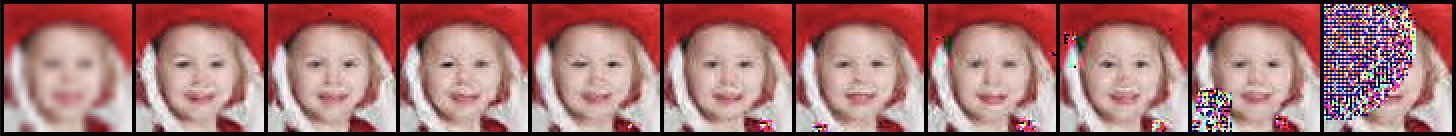
\includegraphics[width=\textwidth]{Chapter1/paper_graphs/10samples_decreasing_conditional_loglikelihood.png}
    \caption{10 super-resolved versions of the LR image in decreasing conditional log-likelihood order.}
    \label{ch1:fig:decreasingloglikelihood}
\end{figure}

We have observed that CAFLOW typically assigns to the ground-truth image higher conditional log-likelihood than any generated sample. Such observation suggests that CAFLOW is a powerful conditional likelihood estimator, and that better samples can be obtained by the use of an optimisation algorithm, which searches for samples with high conditional likelihood. However, we used a simpler inference method in this work: keep the best $N$ out of $M$ generated samples based on the conditional log-likelihood. We empirically found that $M$ should be larger for higher sampling temperatures.

\section{Experiments}\label{ch1:sec:numerics}
In this section we evaluate CAFLOW on three image-to-image translation tasks: image super-resolution, image colorization and image inpainting. Moreover, as ablation for the autoregressive structure in a image super-resolution task, we compare CAFLOW to a model that is conditioned in the normalizing flow latent space, assuming that information is exchanged only between latent spaces having the same dimension, c.f. Section \ref{ch1:subsec:modass} and Figure \ref{ch1:fig:dependencies}. 

We refer the reader to section \ref{ch1:sec:details-of-experiments} in the Appendix for more details about the reported experiments and to section \ref{ch1:sec:extended-visual-results} for extended visual results.

\subsection{Image Super-resolution}
\subsubsection{Ablation of the autoregressive structure}
The idea of conditioning in the normalizing flow latent space was first introduced in \cite{Dual-Glow} to design a conditional likelihood estimator named Dual-Glow. 
The main advantage of CAFLOW compared to Dual-Glow is the autoregressive structure in the latent space that allows to accommodate information exchange at different scales. We confirmed it experimentally by pruning the autoregressive connections and modeling the Dual-Glow component distribution $p(L_i|D_i)$ with a conditional normalizing flow. We named this model Dual-Glow+ as it has the same modeling structure as Dual-Glow with the extra advantage of modeling the component distribution $p(L_i|D_i)$ with a conditional normalizing flow instead of a multidimensional Gaussian distribution as in  \cite{Dual-Glow}. Moreover, we increased the depth of the conditional flow that models $p(L_i|D_i)$, so that Dual-Glow+ and CAFLOW have approximately the same number of parameters. This is important to ensure that improved performance of CAFLOW is the result of the autoregressive modeling structure.

\begin{figure}[h!]
    \begin{center}
    \setlength{\tabcolsep}{0pt}
    \begin{tabular}{cccccc}
        \scriptsize LR   &  \scriptsize Bicubic & \scriptsize Dual-Glow+    &  \scriptsize  \textbf{CAFLOW}     & \scriptsize True \\
          & (x4) & (x4)    & (x4) & 1024x1024 \\
    
    
\includegraphics[width=0.18\linewidth]{Chapter1/paper_graphs/super_resolution/LR.jpg} &
    
\includegraphics[width=0.18\linewidth]{Chapter1/paper_graphs/super_resolution/BICUBIC.jpg} &
    \includegraphics[width=0.18\linewidth]{Chapter1/paper_graphs/super_resolution/Dual-Glow.png} &
    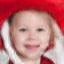
\includegraphics[width=0.18\linewidth]{Chapter1/paper_graphs/super_resolution/CAFLOW.png} &
    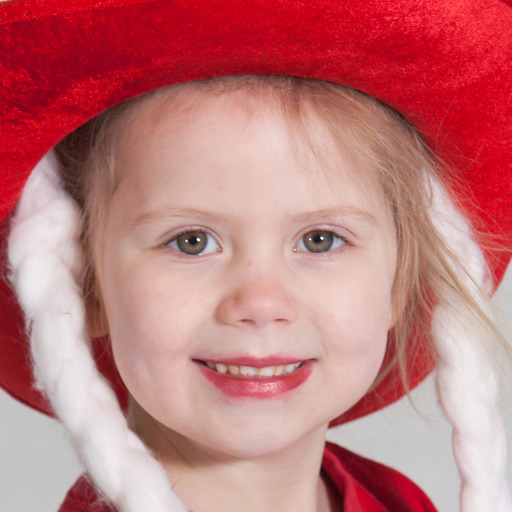
\includegraphics[width=0.18\linewidth]{Chapter1/paper_graphs/super_resolution/TRUE.jpg} \\
    
    \end{tabular}
    \caption{Qualitative comparison of Dual-Glow+ and CAFLOW.}
    \label{ch1:fig:ablation}
    \end{center}
\end{figure}

In Figure \ref{ch1:fig:ablation} we show the qualitative comparison of Dual-Glow+ and CAFLOW on a x4 super-resolution task.  It is apparent that CAFLOW outperforms Dual-Glow+, confirming the significance of allowing exchange of information between different scales. We refer to the next section for more details about the image super-resolution experiment and a quantitative comparison between Dual-Glow+ and CAFLOW, c.f. Table \ref{ch1:comparisonBRGM}.

\subsubsection{Experiment}
We evaluate the ability of CAFLOW and Dual-Glow+ to perform image super-resolution on the FFHQ dataset \cite{karras2019style} (Creative Commons BY-NC-SA 4.0). We resized the original images to $16\times16$ and $64\times 64$ patches and trained the model for x4 super-resolution. The quantitative evaluation is performed using the LPIPS and RMSE scores on 100 unseen images. For inference, we used $\tau=0.5$ and kept the sample with the highest conditional log-likelihood out of ten generated samples. A comparison with state-of-the-art methods is shown in Table \ref{ch1:comparisonBRGM}. We present visual results in Figure \ref{ch1:SR-visuals-paper} and refer the reader to the supplementary material for more examples.

{\footnotesize
\begin{table}[h!]
\centering
\caption{Quantitative evaluation of (x4) super-resolution on FFHQ $16^2$. We report LPIPS/RMSE scores for each method. Lower scores are better.}\label{ch1:comparisonBRGM}
\label{ch1:eval-super-resolution}
\setlength{\tabcolsep}{3pt}


\begin{tabular}{l|cccccc}\label{ch1:tab:one}
 Dataset &    \textbf{CAFLOW} & \textbf{Dual-Glow+} &   BRGM \cite{BRGM}     &   ESRGAN \cite{ESRGAN}    &   SRFBN \cite{li2019feedback}  &  BICUBIC \\

%  & \lpi & \rms  & \lpi & \rms & \lpi & \rms & \lpi & \rms\\
\midrule
   FFHQ $16^2$ &  \textbf{0.08}/\textbf{17.56}  &  \textbf{0.14}/\textbf{18.56} & 0.24/25.66  &  0.35/29.32 &  0.33/22.07 & 0.34/20.10 \\

\end{tabular}
%\vspace{0.1in}
\end{table}
}

\begin{figure}[h!]
    \begin{center}
    \setlength{\tabcolsep}{1pt} % Optional: Adjust the space between images
    \begin{tabular}{cccccccc}
        \scriptsize LR & \scriptsize Bicubic & \scriptsize ESRGAN & \scriptsize SRFBN & \scriptsize BRGM & \scriptsize Dual-Glow+ & \scriptsize \textbf{CAFLOW} & \scriptsize True \\
        & (x4) & (x4) & (x4) & (x4) & (x4) & (x4) & 1024x1024 \\
        
\includegraphics[width=0.12\linewidth]{Chapter1/paper_graphs/super_resolution/LR.jpg} &
        
\includegraphics[width=0.12\linewidth]{Chapter1/paper_graphs/super_resolution/BICUBIC.jpg} &
        
\includegraphics[width=0.12\linewidth]{Chapter1/paper_graphs/super_resolution/ESRGAN.jpg} &
        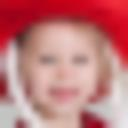
\includegraphics[width=0.12\linewidth]{Chapter1/paper_graphs/super_resolution/SRFBN.jpg} &
        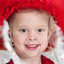
\includegraphics[width=0.12\linewidth]{Chapter1/paper_graphs/super_resolution/BRGM.jpg} &
        \includegraphics[width=0.12\linewidth]{Chapter1/paper_graphs/super_resolution/Dual-Glow.png} &
        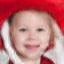
\includegraphics[width=0.12\linewidth]{Chapter1/paper_graphs/super_resolution/CAFLOW.png} &
        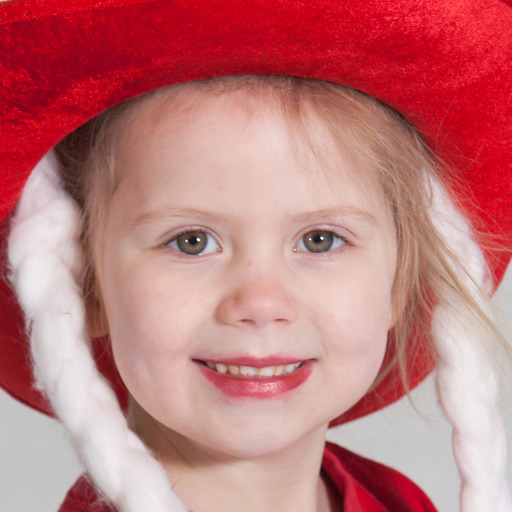
\includegraphics[width=0.12\linewidth]{Chapter1/paper_graphs/super_resolution/TRUE.jpg} \\
    \end{tabular}
    \end{center}
    \caption{Qualitative evaluation on FFHQ 4x super-resolution of 16x16 resolution images.}\label{ch1:SR-visuals-paper}
    \end{figure}
    
    Table \ref{ch1:comparisonBRGM} shows that CAFLOW outperforms Dual-Glow+ based on both metrics, which confirms the theoretical advantage of the autoregressive modeling structure. Moreover CAFLOW outperforms all the other super-resolution methods based on both metrics. It is slightly inferior to BRGM \cite{BRGM} in terms of perceptual quality but it is significantly better in terms of fidelity which is reflected in the quantitative evaluation.


\subsection{Image Colorization}
    To our knowledge, diverse image colorization has been addressed by conditional flows \cite{ardizzone2019guided}, conditional GANs \cite{colorGAN} and recently score-based models \cite{scorebased}. 
    We trained the model on $10\%$ of the LSUN bedroom $64\times 64$ training dataset \cite{yu2015lsun},  a popular dataset for image colorization. For inference, we used $\tau=0.85$ and kept the best out of ten generated samples for each test image using the conditional log-likelihood. We report the performance of the model in Table \ref{ch1:colorisation-comparison}. We use the FID score to compare our method against the cINN and ColorGAN, which have been trained on the full dataset. We show visual results for all methods in Figure \ref{ch1:fig:colorisation-paper-visuals-results}. 
    We did not include \cite{scorebased} in the comparison because it was trained on higher resolution images.

\begin{figure}[h!]
        \begin{center}
        \setlength{\tabcolsep}{3pt}
        %\renewcommand{\arraystretch}{1.5}% Spread rows out...
        \begin{tabular}{ccc}
        CAFLOW & CINN \cite{ardizzone2019guided} & ColorGAN \cite{colorGAN}  \\
        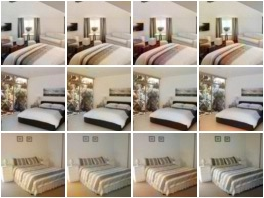
\includegraphics[height=2.9cm]{Chapter1/paper_graphs/colourisation/CAFLOW_borders.png}&
        \includegraphics[height=2.9cm]{Chapter1/paper_graphs/colourisation/CINN.png}&
        \includegraphics[height=2.9cm]{Chapter1/paper_graphs/colourisation/colorGAN.png}\\
        \end{tabular}
        \caption{Qualitative evaluation: Four colorizations proposed by CAFLOW, CINN and ColorGAN for three test images. ColorGAN generates unrealistically diverse colorizations with significant color artifacts (for example a yellow region on a white wall). CINN generates more realistic, less diverse colorizations with fewer pronounced color artifacts compared to ColorGAN, which is reflected in the improved FID score. Finally, CAFLOW generates even more realistic and less diverse colorizations than CINN with even rarer color artifacts, which is more representative of the data distribution according to the FID score.}
        \label{ch1:fig:colorisation-paper-visuals-results}
        \end{center}
\end{figure}

\begin{table}[h!]
    \centering
    
    \caption{Quantitative evaluation of colorization on LSUN BEDROOM $64\times 64$ dataset. We report FID score for each method. Lower scores are better. }
    \label{ch1:colorisation-comparison}
    \setlength{\tabcolsep}{3pt}
    
    \begin{tabular}{l|ccccc}
     Metric &    \textbf{CAFLOW} &   CINN \cite{ardizzone2019guided}     &   ColorGAN \cite{colorGAN}  \\
    
    %  & \lpi & \rms  & \lpi & \rms & \lpi & \rms & \lpi & \rms\\
    \midrule
      FID &  \textbf{18.15} & 26.48 &  28.31 \\
    
    \end{tabular}
    %\vspace{0.1in}
\end{table}

Our model outperforms both methods on image colorization based on the FID metric. We calculated the FID score by generating one conditional sample for each test image, so that our evaluation is identical with the evaluation of the other methods. Moreover, we calculated the FID score by generating 5 samples for each test image, which yielded an improved FID score ($\textbf{16.73}$). We suggest that this protocol be adopted by methods which address diverse image colorization in the future. 

\subsection{Image Inpainting}

We evaluated the performance of CAFLOW on image inpainting by removing central masks covering $25\%$ of the centrally cropped human face of the CelebA dataset \cite{liu2015deep}. We compare the performance of the model with the conditional flow \cite{cGLOW} on the same task using the PSNR metric, see Table \ref{ch1:quantitative-evaluation-inpainting}. We show inpainting examples in Figure \ref{ch1:qualitative-performance-inpainting}.

\begin{figure}[h!]
    \centering
    \includegraphics[width=.8\textwidth]{Chapter1/paper_graphs/inpainting/even_smaller_merged.jpg}
    \caption{Different inpaintings proposed by CAFLOW with $\tau=0.5$. Ground truth on the right.}
    \label{ch1:qualitative-performance-inpainting}
\end{figure}

Our model outperforms \cite{cGLOW} based on the PSNR metric and on qualititative performance. CAFLOW generates realistic images by blending smoothly the conditioning with the synthesized part of the image in contrast to \cite{cGLOW} which generates overly smooth synthesized parts which do not blend well with the surrounding image. Both methods fail in faces which wear sunglasses or face sidewise. We believe that this is attributed to the small number of such training examples.

\begin{table}[h!]
    \centering
    \caption{Quantitative evaluation of inpainting on the CelebA dataset. We report PSNR and LPIPS scores for each method.}\label{ch1:quantitative-evaluation-inpainting}
    \setlength{\tabcolsep}{3pt}
    \begin{tabular}{l|cccc}
     Method  &  PSNR$\uparrow$  &   LPIPS$\downarrow$    \\
    
    \midrule
      \textbf{CAFLOW} &  \textbf{26.08} & 0.06  \\
      \cite{cGLOW} & 24.88 & -
        
    \end{tabular}
    %\vspace{0.1in}
    \end{table}

\section{Conclusion and Limitations}\label{ch1:sec:conclusions}

We have introduced a conditional autoregressive flow, coined CAFLOW, which combines autoregressive modeling with conditional normalizing flows for image-to-image translation. CAFLOW is an efficient conditional image generator and conditional likelihood estimator able to cross-correlate information at different scales, improving on the expressivity of former conditional flow architectures. 
We demonstrate its efficiency as conditional generator on standard image-to-image translation tasks such as image super-resolution, image colorization and image inpainting. We find that, in the above-mentioned tasks, CAFLOW achieves better performance than standard conditional flows and conditional GANs. In particular, we observe that the autoregressive modeling that allows information exchange at different scales, improves on Dual-Glow performances \cite{Dual-Glow}, where correlation is allowed only between latent spaces of the same dimension.

The main modeling limitation of the framework is attributed to limited expressivity of normalizing flows. Each transformation of a normalizing flow has to be invertible with a tractable calculation of the determinant of the Jacobian. This limits the representational power of normalizing flows. However, Wu et al. \cite{wu2020stochastic} claim to overcome expressivity limitations of normalizing flows by combining deterministic invertible functions with stochastic sampling blocks. Therefore, incorporating their proposed stochastic blocks in our conditional autoregressive flows could potentially lead to significant performance improvement. 

\section*{Acknowledgements}
We thank Lynton Ardizzone for informing us about efficient ways to train normalizing flows. We also thank Razvan Marinescu and You Lu for providing help with practical details of the evaluation procedure.

GB acknowledges support from GSK. 
MC acknowledges support from the Royal Society (Newton International Fellowship NIF\textbackslash R1\textbackslash 192048 Minimal partitions as a robustness boost for neural network classifiers).
CE acknowledges support from the Wellcome Innovator Award RG98755. ZK acknowledges funding from the Royal Society (Industry Fellowship), Wellcome Trust (205067/Z/16/Z), Alan Turing Institute and the Alzheimer’s Drug Discovery Foundation.
CBS acknowledges support from the Philip Leverhulme Prize, the Royal Society Wolfson Fellowship, the EPSRC grants EP/S026045/1 and EP/T003553/1, EP/N014588/1, EP/T017961/1, the Wellcome Innovator Award RG98755, the Leverhulme Trust project Unveiling the invisible, the European Union Horizon 2020 research and innovation programme under the Marie Skodowska-Curie grant agreement No. 777826 NoMADS, the Cantab Capital Institute for the Mathematics of Information and the Alan Turing Institute.


%!TEX root = ../thesis.tex
%*******************************************************************************
%****************************** Second Chapter *********************************
%*******************************************************************************

\chapter{Non-Uniform Diffusion Models}\label{Chapter:non-uniform-diffusion-models}

\ifpdf
    \graphicspath{{Chapter2/Figs/Raster/}{Chapter2/Figs/PDF/}{Chapter2/Figs/}}
\else
    \graphicspath{{Chapter2/Figs/Vector/}{Chapter2/Figs/}}
\fi


Diffusion models have emerged as one of the most promising frameworks for deep generative modeling. In this work, we explore the potential of non-uniform diffusion models. We show that non-uniform diffusion leads to multi-scale diffusion models which have similar structure to this of multi-scale normalizing flows. We experimentally find that in the same or less training time, the multi-scale diffusion model achieves better FID score than the standard uniform diffusion model. More importantly, it generates samples $4.4$ times faster in $128\times 128$ resolution. The speed-up is expected to be higher in higher resolutions where more scales are used. Moreover, we show that non-uniform diffusion leads to a novel estimator for the conditional score function which achieves on par performance with the state-of-the-art conditional denoising estimator. Our theoretical and experimental findings are accompanied by an open source library \href{https://github.com/GBATZOLIS/MSDiff}{MSDiff}
which can facilitate further research of non-uniform diffusion models.

\section{Introduction}

\begin{figure}[h]
    \begin{center}
    \begin{tabular}{ccc}
        \scriptsize Original image $x$ & \scriptsize  Observation $y$ &  \scriptsize  Sample from $p_\theta(x|y)$  \\

        \includegraphics[width=.13\textwidth]{Chapter2/samples/teaser/797_x.png} &   
        \includegraphics[width=.13\textwidth]{Chapter2/samples/teaser/797_y.png} &
        \includegraphics[width=.13\textwidth]{Chapter2/samples/teaser/797_1.png}  \\

        \includegraphics[width=.13\textwidth]{Chapter2/samples/teaser/x.png} &   
        \includegraphics[width=.13\textwidth]{Chapter2/samples/teaser/y.png} &
        \includegraphics[width=.13\textwidth]{Chapter2/samples/teaser/DV.png}  \\

        \includegraphics[width=.13\textwidth]{Chapter2/samples/teaser/189_x.png} &   
        \includegraphics[width=.13\textwidth]{Chapter2/samples/teaser/189_y.png} &
        \includegraphics[width=.13\textwidth]{Chapter2/samples/teaser/189_3.png}  \\
    \end{tabular}
    \end{center}
    \caption{Results from our conditional multi-speed diffusive estimator.}
    \label{ch2:fig:_teaser}
\end{figure}

The goal of generative modelling is to learn a  probability distribution from a finite set of samples. This classical problem in statistics has been studied for many decades, but until recently efficient learning of high-dimensional distributions remained impossible in practice. For images, the strong inductive biases of convolutional neural networks have recently enabled the modelling of such distributions, giving rise to the field of deep generative modelling.

Deep generative modelling became one of the central areas of deep learning with many successful applications.
In recent years much progress has been made in unconditional and conditional image generation.
The most prominent approaches are auto-regressive models \cite{bengio2005autoregressive}, variational auto-encoders (VAEs) \cite{kingma2014autoencoding},  normalizing flows \cite{papamakarios2021normalizing} and generative adversarial networks (GANs) \cite{goodfellow2014generative}.

Despite their success, each of the above methods suffers from important limitations. Auto-regressive models allow for likelihood estimation and high-fidelity image generation, but suffer from poor time complexity in high resolutions. VAEs and normalizing flows are less computationally expensive and allow for likelihood estimation, but tend to produce samples of lower visual quality. Moreover, normalizing flows put restrictions on the possible model architectures (requiring invertibility of the network and a Jacobian log-determinant that is computationally tractable), thus limiting their expressivity. While GANs produce state-of-the art quality samples, they don't allow for likelihood estimation and are notoriously hard to train due to training instabilities and mode collapse. 

Recently, score-based \cite{hyvarinen2005score_original} and diffusion-based  \cite{sohldickstein2015diffusion_original} generative models have been revived and improved in \cite{song2020generative_score} and \cite{ho2020denoising}.  
The connection between the two frameworks in discrete-time formulation has been discovered in \cite{vincent2011connection}. 
Recently in \cite{song2021sde}, both frameworks have been unified into a single continuous-time approach based on stochastic differential equations \cite{song2021sde} and are called score-based diffusion models. 
These approaches have recently received a lot of attention, achieving state-of-the-art performance in likelihood estimation \cite{song2021sde} and unconditional image generation \cite{dhariwal2021diffusion_beats_gans}, surpassing even the celebrated success of GANs.

In addition to achieving state-of-the art performance in both image generation and likelihood estimation, score-based diffusion models don't suffer from training instabilities or mode collapse \cite{dhariwal2021diffusion_beats_gans, song2021sde}. However, although their time complexity in high resolutions is better than that of auto-regressive models \cite{dhariwal2021diffusion_beats_gans}, it is still notably worse to that of GANs, normalizing flows and VAEs. Despite the recent efforts to close the sampling time gap between diffusion models and the faster frameworks, diffusion models still require significantly more time to achieve equal performance.

In this work, we explore non-uniform diffusion models. In non-uniform diffusion models, different parts of the input tensor diffuse with different diffusion speeds or more generally according to different stochastic differential equations. We find that the generalization of the original uniform diffusion framework can lead to multi-scale diffusion models which achieve improved sampling performance at a significantly faster sampling speed.

Moreover, we find that non-uniform diffusion can be used for conditional generation, because it leads to a novel estimator of the conditional score. We conduct a review and classification of existing approaches and perform a systematic comparison to find the best way of estimating the conditional score. We provide a proof of validity for the \textit{conditional denoising estimator} (which has been used in \cite{saharia2021sr3,tashiro2021csdi} without justification), and we thereby provide a firm theoretical foundation for using it in future research.

\noindent
\textbf{The contributions of this paper are as follows:}
\begin{enumerate}
    \item We introduce a principled objective for training non-uniform diffusion models.
    \item We show that non-uniform diffusion leads to the multi-scale diffusion models which are more efficient than uniform diffusion models. In less training time, the multi-scale models reach improved FID scores with significantly faster sampling speed. The speed up factor is expected to increase as we increase the number of scales.
    \item We show that non-uniform diffusion leads to \textit{conditional multi-speed diffusive estimator} (CMDE), a novel estimator of conditional score, which unifies previous methods of conditional score estimation.
    \item We provide a proof of consistency for the \textit{conditional denoising estimator} - one of the most successful approaches to estimating the conditional score. 
    
    \item We review and empirically compare score-based diffusion  approaches to modelling conditional distributions of image data. The models are evaluated on the tasks of super-resolution, inpainting and edge to image translation.

    \item We provide an open-source library \href{https://github.com/GBATZOLIS/conditional_score_diffusion}{MSDiff}, to facilitate further research on conditional and non-uniform diffusion models.
\end{enumerate}

\section{Notation}

In this work we will use the following notation:
\begin{itemize}
    \item \textbf{Functions of time}
    \begin{gather*}
        f_t := f(t)
    \end{gather*}
    \item \textbf{Indexing vectors} \\
    Let $v = (v_1, ..., v_n) \in \mathbb{R}^n$ and let $ 1 \leq i < j < n$. Then:
    \begin{align*}
        %v[i,j] &:= (v_i, v_{i+1}, ..., v_j) \in \mathbb{R}^{j - i + 1} \\ \nonumber
        v[:j] &:= (v_1, v_{2}, ..., v_j) \in \mathbb{R}^{j},
    \end{align*}
    cf. Section \ref{ch2:sec:CDiffE}.
    \item \textbf{Probability distributions} \\
    We denote the probability distribution of a random variable solely via the name of its density's argument, e.g.
    \begin{gather*}
        p(x_t) := p_{X_t}(x_t),
    \end{gather*}   
    where $x_t$ is a realisation of the random variable $X_t$.
    \item \textbf{Iterated Expectations}
    %\begin{gather*}
    %    \mathbb{E}_{\subalign{&x \sim p(x) \\ &y \sim p(y)}}[f(x,y)] := \mathbb{E}_{x \sim p(x)}\mathbb{E}_{y \sim p(y)}[f(x,y)]
    %\end{gather*}
    \begin{align*}
        &\mathbb{E}_{\subalign{z_1 &\sim p(z_1) \\ &{\myvdots} \\z_n &\sim p(z_n)}}[f(z_1,\Compactcdots,z_n)] \\
        :=&\mathbb{E}_{z_1 \sim p(z_1)} \Compactcdots \mathbb{E}_{z_n \sim p(z_n)}[f(z_1,\Compactcdots,z_n)]
    \end{align*}
\end{itemize} 

\section{Methods}
In the following, we will provide details about the framework and estimators discussed in this paper.
\subsection{Background: Score matching through Stochastic Differential Equations}
\subsubsection{Score-Based Diffusion}


In a recent work \cite{song2021sde} score-based  \cite{hyvarinen2005score_original, song2020generative_score} and diffusion-based \cite{sohldickstein2015diffusion_original, ho2020denoising} generative models have been unified into a single continuous-time score-based framework where the diffusion is driven by a stochastic differential equation.  This framework relies on Anderson's Theorem \cite{anderson1982reverse_time_sde}, which states that under certain Lipschitz conditions on $f : \mathbb{R}^{n_x} \times \mathbb{R} \xrightarrow{} \mathbb{R}^{n_x}$ and $G : \mathbb{R}^{n_x} \times \mathbb{R}\xrightarrow{} \mathbb{R}^{n_x} \times \mathbb{R}^{n_x}$ and an integrability condition on the target distribution $p(\textbf{x}_0)$ a forward diffusion process governed by the following SDE:
\begin{equation}
    \label{ch2:eq:forward_sde}
    d\mathbf{x}_t = f(\mathbf{x}_t, t) \, dt + G(\mathbf{x}_t, t) \, d\mathbf{w}_t
\end{equation}
has a reverse diffusion process governed by the following SDE:
\begin{equation}
    \label{ch2:eq:reverse_sde}
    d\mathbf{x}_t = \left[f(\mathbf{x}_t, t) - G(\mathbf{x}_t, t) G(\mathbf{x}_t, t)^T \nabla_{\mathbf{x}_t} \ln p_{\mathbf{X}_t}(\mathbf{x}_t) \right] dt + G(\mathbf{x}_t, t) \, d\Bar{\mathbf{w}_t}
\end{equation}

\noindent where $\Bar{\textbf{w}_t}$ is a standard Wiener process in reverse time. 

The forward diffusion process transforms the \textit{target distribution} $p(\textbf{x}_0)$ to a \textit{diffused distribution} $p(\textbf{x}_T)$ after diffusion time $T$. By appropriately selecting the drift and the diffusion coefficients of the forward SDE, we can make sure that after sufficiently long time $T$, the diffused distribution $p(\textbf{x}_T)$ approximates a simple distribution, such as $\mathcal{N}(\textbf{0},\textbf{I})$. We refer to this simple distribution as the \textit{prior distribution}, denoted by $\pi$. The reverse diffusion process transforms the diffused distribution $p(\textbf{x}_T)$ to the data distribution $p(\textbf{x}_0)$ and the prior distribution $\pi$ to a distribution $p^{SDE}$. $p^{SDE}$ is close to $p(\textbf{x}_0)$ if the diffused distribution $p(\textbf{x}_T)$ is close to the prior distribution $\pi$. We get samples from $p^{SDE}$ by sampling from $\pi$ and simulating the reverse sde from time $T$ to time $0$.

To get samples by simulating the reverse SDE, we need access to the time-dependent score function $\nabla_{\textbf{x}_t}{\ln{p(\textbf{x}_t)}}$ for all $\textbf{x}_t$ and $t$. In practice, we approximate the time-dependent score function with a neural network $s_{\theta}(\textbf{x}_t,t) \approx \nabla_{\textbf{x}_t}{\ln{p(\textbf{x}_t)}}$ and simulate the reverse SDE in equation \ref{ch2:eq:approximated_reverse_sde} to map the prior distribution $\pi$ to $p^{SDE}_{\theta}$.

\begin{equation}
    \label{ch2:eq:approximated_reverse_sde}
    d\mathbf{x}_t = \left[ f(\mathbf{x}_t, t) - G(\mathbf{x}_t, t) G(\mathbf{x}_t, t)^T s_{\theta}(\mathbf{x}_t, t) \right] dt + G(\mathbf{x}_t, t) \, d\Bar{\mathbf{w}_t}
\end{equation}

If the prior distribution is close to the diffused distribution and the approximated score function is close to the ground truth score function, the modeled distribution  $p^{SDE}_{\theta}$ is provably close to the target distribution $p(\textbf{x}_0)$. This statement is formalised in the language of distributional distances in the next subsection.

\subsubsection{Uniform Diffusion Models}
Previous works \cite{ho2020denoising, song2020generative_score, dhariwal2021diffusion_beats_gans} used the same forward SDE for the diffusion of all the pixels. For this reason, we classify them as uniform diffusion models. In uniform diffusion models, the sde in equation \ref{ch2:eq:uniform_sde} describes the forward diffusion for all pixels in an image:

\begin{equation}\label{ch2:eq:uniform_sde}
dx_t=f(x_t,t)dt + g(t)d\Bar{w_t},
\end{equation}

We used unbold notation for the random variables to show that this equation describes diffusion in one dimension. For uniform diffusion models, the neural network $s_\theta(\textbf{x}_t,t)$ can be trained to approximate the score function $\nabla_{\textbf{x}_t}{\ln{p(\textbf{x}_t)}}$ by minimizing the weighted score matching objective
\begin{gather}
    \mathcal{L}_{SM}(\theta, \lambda(\cdot)) := \frac{1}{2} \mathbb{E}_{\subalign{&t \sim U(0,T)\\ &\textbf{x}_t \sim p(\textbf{x}_t)}} [\lambda(t) \norm{\nabla_{\textbf{x}_t}{\ln{p(\textbf{x}_t)}} - s_\theta(\textbf{x}_t,t)}_2^2]
\end{gather}
where $\lambda: [0,T] \xrightarrow{} \mathbb{R}_+$ is a positive weighting function.

However, the above quantity cannot be optimized directly since we don't have access to the ground truth score $\nabla_{\textbf{x}_t}{\ln{p(\textbf{x}_t)}}$. Therefore in practice, a different objective has to be used \cite{hyvarinen2005score_original, song2020generative_score, song2021sde}. In \cite{song2021sde}, the weighted denoising score-matching objective is used, which is defined as 

\begin{equation}
    \label{ch2:DSM for uniform diffusion_models}
    \mathcal{L}_{DSM}(\theta, \lambda(\cdot)) := \frac{1}{2} \mathbb{E}_{\substack{t \sim U(0,T) \\ \mathbf{x}_0 \sim p(\mathbf{x}_0) \\ \mathbf{x}_t \sim p(\mathbf{x}_t | \mathbf{x}_0)}}
    \left[\lambda(t) \left\| \nabla_{\mathbf{x}_t} \ln{p(\mathbf{x}_t | \mathbf{x}_0)} - s_\theta(\mathbf{x}_t,t) \right\|_2^2 \right]
\end{equation}
    

The difference between DSM and SM is the replacement of the ground truth score which we do not know by the score of the perturbation kernel which we know analytically for many choices of forward SDEs. The choice of the weighted DSM objective is justified because the weighted DSM objective is equal to the SM objective up to a constant that does not depend on the parameters of the model $\theta$. The reader can refer to \cite{vincent2011connection} for the proof. 

The choice of the weighting function is also important, because it determines the quality of score-matching in different diffusion scales. A principled choice for the weighting function is $\lambda(t) = g(t)^2$, where $g(\cdot)$ is the diffusion coefficient of the forward SDE. This weighting function is called the likelihood weighting function \cite{song2021maximum}, because it ensures that we minimize an upper bound on the Kullback–Leibler divergence from the target distribution to the model distribution by minimizing the weighted DSM objective with this weighting. The previous statement is implied by the combination of inequality \ref{ch2:Likelihood Weighting for Uniform Diffusion_Models} which is proven in \cite{song2021maximum} and the relationship between the DSM and SM objectives.

\begin{equation}\label{ch2:Likelihood Weighting for Uniform Diffusion_Models}
D_{KL}(p(\textbf{x}_0)\parallel p^{SDE}_{\theta})\leq L_{SM}(\theta, g(\cdot)^2)+D_{KL}(p(\textbf{x}_T)\parallel \pi)
\end{equation}

Other weighting functions have also yielded very good results with particular choices of forward sdes. However, we do not have theoretical guarantees that alternative weightings would yield good results with arbitrary choices of forward sdes.


\subsection{Non-Uniform Diffusion Models}\label{ch2:Non-Uniform Diffusion_Models}
In this section, we describe non-uniform diffusion models. We call them non-uniform to indicate that the forward diffusion of each pixel is potentially governed by a different SDE. Considering a vectorised form $x=\text{vec}(X)=[x^1, x^2,...,x^{mnc}]$ of an image $X\in [0,1]^m\times[0,1]^n\times[0,1]^c$, we assume that the diffusion of the $i^{th}$ pixel is governed by the following SDE:

\begin{equation}\label{ch2:non-uniform pixel_diffusion}
    dx^{i}_t = f_i(x^i_t,t)dt+g_i(t)dw^i_t
\end{equation}

Equation \ref{ch2:non-uniform pixel_diffusion} is a special case of the general It\^{o} SDE described in equation \ref{ch2:eq:forward_sde}, but provides more flexibility compared to uniform diffusion where all pixels diffuse independently according to the same SDE. The diffusion of the entire image vector is summarised by the following SDE:

\begin{equation}\label{ch2:non-uniform image_diffusion}
    d\textbf{x}_t = f(\textbf{x}_t,t)dt+G(t)d\textbf{w}_t,
\end{equation}

\noindent where \(f(\textbf{x}_t)=[f_1(x^1,t),...,f_{mnc}(x^{mnc}_t,t)]\) and \(G(t)=\text{diag}([g_1(t),...,g_{mnc}(t)])\).

In this more general setup, the DSM objective as described in equation \ref{ch2:DSM for uniform diffusion_models} must also be generalised. The positive weighting function $\lambda(\cdot)$ is replaced by a positive definite matrix $\Lambda(\cdot)$ which gives the form of the DSM objective for non-uniform diffusion models:

\begin{equation}
    \label{ch2:DSM for non-uniform diffusion_models}
    \mathcal{L}_{DSM}(\theta, \Lambda(\cdot)) := \frac{1}{2} \mathbb{E}_{\substack{t \sim U(0,T) \\ \mathbf{x}_0 \sim p(\mathbf{x}_0) \\ \mathbf{x}_t \sim p(\mathbf{x}_t | \mathbf{x}_0)}}
    \left[ \mathbf{v}_{\theta}(\mathbf{x}_0, \mathbf{x}_t, t)^T \Lambda(t) \mathbf{v}_{\theta}(\mathbf{x}_0, \mathbf{x}_t, t) \right]
\end{equation}
    

\noindent where \(\textbf{v}_{\theta}(\textbf{x}_0,\textbf{x}_t,t)=\nabla_{\textbf{x}_t}{\ln{p(\textbf{x}_t | \textbf{x}_0)}} - s_\theta(\textbf{x}_t,t)\)

We prove that a principled choice for the positive weighting matrix is $\Lambda_{MLE}(t)=G(t)G(t)^T$. We call it the likelihood weighting matrix for non-uniform diffusion because it ensures minimization of an upper bound to the KL divergence from the target distribution to the model distribution. The previous statement is summarised in Theorem \ref{ch2:Likelihood Weighting for Non-uniform_diffusion} which is proved in section \ref{ch2:appendix:weighting} of the Appendix.

\begin{theorem}\label{ch2:Likelihood Weighting for Non-uniform_diffusion}
    Let $p(\mathbf{x}_t)$ denote the distribution implied by the forward SDE at time $t$ and $p^{SDE}_\theta(\mathbf{x}_t)$ denote the distribution implied by the parametrized reverse SDE at time $t$. Then under regularity assumptions of \cite[Theorem 1]{song2021maximum}, we have that
    \[
    KL(p(\mathbf{x}_0) \| p^{SDE}_\theta(\mathbf{x}_0)) \leq KL(p(\mathbf{x}_T) \| \pi(\mathbf{x}_T)) + \frac{1}{2} \mathbb{E}_{\substack{t \sim U(0,T) \\ \mathbf{x}_t \sim p(\mathbf{x}_t)}} \left[ \mathbf{v}^T G(t) G(t)^T \mathbf{v} \right],
    \]
    where $\mathbf{v} = \nabla_{\mathbf{x}_t} \ln{p(\mathbf{x}_t)} - s_\theta(\mathbf{x}_t, t)$.
\end{theorem}


\subsection{Application of Non-Uniform Diffusion in multi-scale diffusion} \label{ch2:sec:multi-scale_diffusion}

We design the forward process so that different groups of pixels diffuse with different speeds which creates a multi-scale diffusion structure. The intuition stems from multi-scale normalising flows. Multi-scale normalising flows invertibly transform the input tensor to latent encodings of different scales by splitting the input tensor into two parts after transformation in each scale. The multi-scale structure in normalising flows is shown to lead to faster training and sampling without compromise in generated image quality. %This is because we do not need to transform the entire tensor in all the invertible layers.

We intend to transfer this idea to score-based modeling by diffusing some parts of the tensor faster. There are many ways to split the image into different parts which diffuse faster. It has been experimentally discovered that cascaded diffusion models \cite{saharia2021sr3} yield improved results  compared to standard diffusion models. This gave us the intuition to use a multi-level haar transform to transform every image to $n$ high frequency scales $d_1,...,d_n$ (detail coefficients) and one low frequency scale $a_n$ (approximation coefficient). The natural generation order of the haar coefficients (in line with cascaded diffusion) is $a_n$, $d_n$, $d_{n-1}$, ..., $d_1$. For this reason, we choose to diffuse lower frequency coefficients slower than high frequency coefficients. More specifically, we design the forward process so that all coefficients reach the same signal-to-noise ratio at the end of their diffusion time. We set the diffusion time for $a_n$ to $T_{a_n}=1$ and for $d_i$ to $T_{d_i}=\frac{i}{n+1}$ for each $i\in [1,...,n]$. We illustrate the multiscale model structure graphically in Figure \ref{ch2:fig:Multiscale_model}.

\begin{figure*}[h]
    \centering
    \includegraphics[width=0.9\textwidth]{Chapter2/samples/multiscale/drawing.png}
    \caption{Model with three scales. $d_1$ reaches the target SNR at $t=0.25$ and does not diffuse further. The remaining part of tensor continues the diffusion. The diffusion procedure is continued as implied until $a_3$ reaches the target SNR at time $t=1$. We use four neural networks $S_1, S_2, S_3, S_4$ to approximate the score function in the intermediate diffusion intervals, because the dimensionality of the diffusing tensor decreases every time some part of the tensor reaches the target SNR.}
    \label{ch2:fig:Multiscale_model}
\end{figure*}

\subsubsection{Training}
We approximate the score of the distribution of $c_i(t) = [a_n(t), d_n(t),...,d_i(t)]$ in the time range $[(i-1)/(n+1), i/(n+1)]$ with a separate neural network $s_i(c_i(t), t)$. We also use a separate network $s_{n+1}(c_{n+1}(t), t)$ to approximate the score of the distribution of $c_{n+1}(t)=a_n(t)$ in the diffusion time range $[n/(n+1), 1]$. We use different networks in each scale to leverage the fact that we approximate the score of lower dimensional distributions. This enables faster score function evaluation and, therefore, faster training and sampling. We train each network separately using the likelihood weighting matrix for non-uniform diffusion (see section \ref{ch2:Non-Uniform Diffusion_Models}).

\subsubsection{Sampling}
The sampling process is summarised in the following steps:

\begin{enumerate}
    \item  Sample $a_n(1)$ from the stationary distribution (e.g. standard normal distribution) and integrate the reverse sde for $a_n$ from time $t=1$ to time $t=n/(n+1)$. 
    \item Sample $d_n(n/(n+1))$ from the stationary distribution and solve the reverse sde for $[a_n, d_n]$ from time $t=n/(n+1)$ to time $t=(n-1)/(n+1)$.
    \item The process is continued as implied until we reach the final generation level, where we sample $d_1(1/(n+1))$ from the stationary distribution and solve the reverse sde for $[a_n,d_n,...,d_1]$ from time $t=1/(n+1)$ to time $t=\epsilon$ (e.g., $\epsilon=10^{-5}$). 
    \item We convert the generated haar coefficients $[a_n(\epsilon),d_n(\epsilon),...,d_1(\epsilon)]$ to the generated image using the multi-level inverse haar transform.
\end{enumerate}

Our experimental results presented in section \ref{ch2:Multiscale diffusion_experiments} show that multiscale diffusion is more efficient and effective than uniform diffusion.

%We present the results on ImageNet and CelebA which show that for the same number of parameters and the same training time, the multi-scale model achieves better performance with faster sampling speed.

\subsection{Application of Non-Uniform Diffusion in Conditional generation} \label{ch2:sec:conditional_generation}

The continuous score-matching framework can be extended to conditional generation, as shown in  \cite{song2021sde}. Suppose we are interested in $p(x|y)$, where $x$ is a \textit{target image} and $y$ is a \textit{condition image}. Again, we use the forward diffusion process (Equation \ref{ch2:eq:forward_sde}) to obtain a family of diffused distributions $p(x_t | y)$ and apply Anderson's Theorem to derive the \textit{conditional reverse-time SDE}
\begin{equation}
    \label{ch2:eq:conditional_reverse_sde}
    dx = [\mu(x,t) - \sigma(t)^2 \nabla_{x} \ln p_{X_t}(x | y)]dt + \sigma(t)d\tilde{w}.
\end{equation}
Now we need to learn the score $\nabla_{x_t} \ln p(x_t|y)$ in order to be able to sample from $p(x | y)$ using reverse-time diffusion.\\

In this work, we discuss the following approaches to estimating the conditional score $\nabla_{x_t} \ln p(x_t|y)$:
\begin{enumerate}
    \item Conditional denoising estimators
    \item Conditional diffusive estimators
    \item Multi-speed conditional diffusive estimators (our method)
\end{enumerate}
We discuss each of them in a separate section.\\

In \cite{song2021sde} an additional approach to conditional score estimation was suggested:
This method proposes learning $\nabla_{x_t} \ln p(x_t)$ with an unconditional score model, and  learning $p(y | x_t)$ with an auxiliary model. Then, one can use 
    \begin{equation*}
        \nabla_{x_t}\ln p(x_t |y) = \nabla_{x_t} \ln p(x_t) + \nabla_{x_t} \ln p(y | x_t)
    \end{equation*}
to obtain $\nabla_{x_t} \ln p(x_t | y)$. Unlike other approaches, this requires training a separate model for $p(y|x_t)$. Appropriate choices of such models for tasks discussed in this paper have not been explored yet. Therefore we exclude this approach from our study. 

\subsubsection{Conditional denoising estimator (CDE)}
The conditional denoising estimator (CDE) is a way of estimating $p(x_t|y)$ using the denoising score matching approach \cite{vincent2011connection, song2020generative_score}. In order to approximate $p(x_t|y)$, the conditional denoising estimator minimizes
\begin{gather}
\begin{aligned}
        \label{ch2:CDN}
        &\frac{1}{2} \mathbb{E}_{\subalign{&t \sim U(0,T)\\ &x_0, y \sim p(x_0, y) \\ &x_t \sim p(x_t | x_0)}} 
        [\lambda(t) \norm{\nabla_{x_t} \ln{p(x_t | x_0)} - s_\theta(x_t, y, t)}_2^2]
\end{aligned}
\end{gather}
This estimator has been shown to be successful in previous works \cite{saharia2021sr3,tashiro2021csdi}, also confirmed in our experimental findings (cf. Section \ref{ch2:sec:experiments}). 

Despite the practical success, this estimator has previously been used without a theoretical justification of why training the above objective yields the desired conditional distribution. Since $p(x_t|y)$ does not appear in the training objective, it is not obvious that the minimizer approximates the correct quantity. 

By extending the arguments of \cite{vincent2011connection}, we provide a formal proof that the minimizer of the above loss does indeed approximate the correct conditional score $p(x_t|y)$. This is expressed in the following theorem.

\begin{theorem}
    \label{ch2:thm:CDE_consistency}
    The minimizer (in $\theta$) of
    \begin{gather*}
    \begin{aligned}
            \frac{1}{2} \mathbb{E}_{\subalign{&t \sim U(0,T)\\ &x_0, y \sim p(x_0, y) \\ &x_t \sim p(x_t | x_0)}} 
            [\lambda(t) \norm{\nabla_{x_t} \ln{p(x_t | x_0)} - s_\theta(x_t, y, t)}_2^2]
    \end{aligned}
    \end{gather*}    
    is the same as the minimizer of 
    \begin{gather*}
        \frac{1}{2} \mathbb{E}_{\subalign{&t \sim U(0,T)\\ &x_t, y \sim p(x_t, y)}} 
        [\lambda(t) \norm{\nabla_{x_t} \ln{p(x_t | y)} - s_\theta(x_t, y,t)}_2^2]
    \end{gather*}
\end{theorem}
\noindent
The proof for this statement can be found in Appendix \ref{ch2:appendix:minimizers}. 
Using the above theorem, the consistency of the estimator can be established.
\begin{corollary}
    Let $\theta^\ast$ be a minimizer of a Monte Carlo approximation of (\ref{ch2:CDN}), then (under technical assumptions, cf. Appendix \ref{ch2:appendix:consistency}) the conditional denoising estimator $s_{\theta^\ast}(x,y,t)$ is a consistent estimator of the conditional score $\nabla_{x_t} \ln p(x_t | y)$, i.e.
    \begin{gather*}
        s_{\theta^\ast}(x,y,t) \overset{P}{\to} \nabla_{x_t} \ln p(x_t | y)   
    \end{gather*}
    as the number of Monte Carlo samples approaches infinity.
\end{corollary}
\noindent
This follows from the previous theorem and the uniform law of large numbers. Proof in the Appendix \ref{ch2:appendix:consistency}.

\subsubsection{Conditional diffusive estimator (CDiffE)}
\label{ch2:sec:CDiffE}
Conditional diffusive estimators (CDiffE) have first been suggested in \cite{song2021sde}. The core idea is that instead of learning $p(x_t | y)$ directly, we diffuse both $x$ and $y$ and approximate $p(x_t | y_t)$, using the denoising score matching. Just like learning diffused distribution $\nabla_{x_t} \ln p(x_t)$ improves upon direct estimation of $\nabla_{x} \ln p(x)$ \cite{song2020generative_score, song2021sde}, diffusing both the input $x$ and condition $y$, and then learning $\nabla_{x_t} \ln p(x_t | y_t)$ could make optimization easier and give better results than learning  $\nabla_{x_t} \ln p(x_t | y)$ directly.
    
In order to learn $p(x_t | y_t)$, observe that
\begin{gather*}
    \nabla_{x_t}\ln p(x_t | y_t) = \nabla_{x_t}\ln p(x_t, y_t) = \nabla_{z_t}\ln p(z_t)[:n_x],
\end{gather*}
where $z_t := (x_t, y_t)$ and $n_x$ is the dimensionality of $x$. Therefore we can learn the (unconditional) score of the joint distribution $p(x_t, y_t)$ using the denoising score matching objective just like as in the unconditional case, i.e
\begin{gather}
    \label{ch2:CDF}
\begin{aligned}
    &\frac{1}{2} \mathbb{E}_{\subalign{&t \sim U(0,T)\\ &z_0 \sim p_0(z_0) \\ &z_t \sim p(z_t | z_0)}} [\lambda(t) \norm{\nabla_{z_t} \ln{p(z_t |z_0)} - s_\theta(z_t,t)}_2^2].
\end{aligned}
\end{gather}
We can then extract our approximation for the conditional score $\nabla_{x_t} \ln p(x_t|y_t)$ by simply taking the first $n_x$ components of $s_\theta(x_t, y_t,t)$.

The aim is to approximate $\nabla_{x_t} \ln p(x_t | y)$ with $\nabla_{x_t} \ln p(x_t|\hat{y_t})$, where $\hat{y}_t$ is a sample from $p(y_t | y)$. Of course this approximation is imperfect and introduces an error, which we call the \textit{approximation error}. CDiffE aims to achieve smaller optimization error by diffusing the condition $y$ and making the optimization landscape easier, at a cost of making this approximation error.

Now in order to obtain samples from the conditional distribution, we sample a point $x_T \sim \pi$ and integrate
\begin{gather*}
    dx = [\mu(x,t) - \sigma(t)^2 \nabla_{x} \ln p_{X_t|Y_t}(x | \hat{y}_t)]dt + \sigma(t)d\tilde{w}
\end{gather*}
from $T$ to $0$, sampling $\hat{y}_t \sim p(y_t | y)$ at each time step.

% For completeness, we state formally the consistency of the conditional diffusive estimator.

% \begin{theorem}
%     Let $\theta^\ast$ be a minimizer of a Monte Carlo approximation of \ref{ch2:CDF}. Then assuming a sufficient model capacity, the conditional denoising estimator $s_{\theta^\ast}(x,y,t)[:n_x]$ is a consistent estimator of the diffused conditional score $\nabla_{x_t} \ln p(x_t | y_t)$ i.e.
%     \begin{gather*}
%         s_{\theta^\ast}(x,y,t)[:n_x] \overset{P}{\to} \nabla_{x_t} \ln p(x_t | y_t)   
%     \end{gather*}
%     as the number of Monte Carlo samples approaches infinity.
% \end{theorem}
% The above follows form the fact that $\argmin_\theta \mathcal{L}_\text{SM}(\theta) = \argmin_\theta \mathcal{L}_\text{DSM}(\theta)$ \cite{vincent2011connection} and the uniform law of large numbers. See Appendix \ref{ch2:appendix:proofs} for technical details.


\subsubsection{Conditional multi-speed diffusive estimator (CMDE)}
\label{ch2:sec:CMDE}
\begin{figure}
\begin{mdframed}
    \begin{center}
       \textbf{Sources of error for different estimators}
    \end{center}
    \textbf{CDE}\\
    Optimization error:
    \begin{gather*}
    s_\theta(x,y,t) \approx \nabla_{x_t}\ln p(x_t|y)   
    \end{gather*}
    \textbf{CDiffE and CMDE}\\
    Optimization error:
    \begin{gather*}
        s_\theta(x,y,t) \approx \nabla_{x_t}\ln p(x_t|y_t)   
        \end{gather*}
    Approximation error:
    \begin{gather*}
        \nabla_{x_t}\ln p(x_t|\hat{y}_t) \approx \nabla_{x_t}\ln p(x_t|y)   
        \end{gather*}
    CDiffE aims to achieve smaller optimization error at a cost of higher approximation error. By controlling the diffusion speed of $y$, CMDE tries to find an optimal balance between optimization error and approximation error.
\end{mdframed}
\caption{Sources of error for different estimators}
\label{ch2:fig:box}
\end{figure}
In this section we present a novel estimator for the conditional score $\nabla_{x_t} \ln p(x_t | y)$ which we call the \textit{conditional multi-speed diffusive estimator} (CMDE). 

Our approach is based on two insights. Firstly, there is no reason why $x_t$ and $y_t$ in conditional diffusive estimation need to diffuse at the same rate. Secondly, by decreasing the diffusion rate of $y_t$ while keeping the diffusion speed of $x_t$ the same, we can bring $p(x_t |y_t)$ closer to $p(x_t |y)$, at the possible cost of making the optimization more difficult. This way we can \emph{interpolate} between the conditional denoising estimator and the conditional diffusive estimator and find an optimal balance between optimization error and approximation error (cf. Figure \ref{ch2:fig:box}). This can lead to a better performance, as indicated by our experimental findings (cf. Section \ref{ch2:sec:experiments}).

In our conditional multi-speed diffusive estimator, $x_t$ and $y_t$ diffuse according to SDEs with the same drift but different diffusion rates,
\begin{gather*}
    dx = \mu(x,t)dt+\sigma^x(t)dw  \\
    dy = \mu(y,t)dt+\sigma^y(t)dw.
\end{gather*}


Then, just like in the case of conditional diffusive estimator, we try to approximate the joint score $\nabla_{x_t, y_t} \ln p(x_t, y_t)$ with a neural network. Since $x_t$ and $y_t$ now diffuse according to different SDEs, we need to take this into account and replace the weighting function $\lambda(t):\mathbb{R} \xrightarrow{} \mathbb{R}_+ $ with a positive definite weighting matrix $\Lambda(t): \mathbb{R} \xrightarrow{} \mathbb{R}^{(n_x + n_y) \times (n_x + n_y)}$. Hence, the new training objective becomes
\begin{gather}
    \label{ch2:eq:CMDE}
    \begin{aligned}
        \frac{1}{2} \mathbb{E}_{\subalign{&t \sim U(0,T)\\ &z_0 \sim p_0(z_0) \\ &z_t \sim p(z_t | z_0)}} 
        [
            v^T \Lambda(t) v
        ],
    \end{aligned}
\end{gather}
where $v=\nabla_{z_t} \ln{p(z_t |z_0)} - s_\theta(z_t,t)$, $z_t=(x_t,y_t)$.

In \cite{song2021maximum} authors derive a likelihood weighting function $\lambda^{\text{MLE}}(t)$, which ensures that the objective of the score-based model upper-bounds the negative log-likelihood of the data, thus enabling approximate maximum likelihood training of score-based diffusion models. We generalize this result to the multi-speed diffusion case by providing a likelihood weighting matrix $\Lambda^{\text{MLE}}(t)$ with the same properties.

\begin{theorem}
    \label{ch2:thm:weightning}
    Let $\mathcal{L}(\theta)$ be the CMDE training objective (Equation \ref{ch2:eq:CMDE}) with the following weighting:
    \begin{gather*}
        \Lambda^{\text{MLE}}_{i,j}(t) =  
        \begin{cases} 
            \sigma^x(t)^2, \text{ if } i=j, \ i \leq n_x \\ 
            \sigma^y(t)^2, \text{ if } i=j, \ n_x < i \leq n_y  \\
            0, \text{ otherwise}
        \end{cases}            
    \end{gather*}
    Then the joint negative log-likelihood is upper bounded (up to a constant in $\theta$) by the training objective of CMDE
    \begin{gather*}
        -\mathbb{E}_{(x,y) \sim p(x,y)}[\ln p_\theta(x,y)] \leq \mathcal{L}(\theta) + C.
    \end{gather*}
\noindent
\end{theorem}

\noindent
The proof can be found in Appendix \ref{ch2:appendix:weighting}. 

Moreover we show that the mean squared approximation error of a multi-speed diffusion model is upper bounded and the upper bound goes to zero as the diffusion speed of the condition $\sigma^y(t)$ approaches zero.
\begin{theorem}
    Fix $t$, $x_t$ and $y$. Under mild technical assumptions (cf. Appendix \ref{ch2:appendix:mse}) there exists a function  $E: \mathbb{R} \xrightarrow{} \mathbb{R}$ monotonically decreasing to $0$, such that
    \begin{gather*}
        \mathbb{E}_{y_t \sim p(y_t|y)}[
            \norm{ \nabla_{x_t} \ln p(x_t|y_t) - \nabla_{x_t} \ln p(x_t|y)}_2^2
            ] \\
            \leq E(1/\sigma^y(t)).
    \end{gather*}
\end{theorem}
\noindent
The proof can be found in Appendix \ref{ch2:appendix:mse}.

Thus we see that the objective of CMDE approaches that of CDE as  $\sigma^y(t) \to 0$, and  CMDE coincides with CDiffE when $ \sigma^y(t) = \sigma^x(t)$ (cf. Figure \ref{ch2:fig:box}).

We experimented with different configurations of $\sigma^x(t)$ and $\sigma^y(t)$ and found configurations that lead to  improvements upon CDiffE and  CDE in certain tasks. The experimental results are discussed in detail in Section \ref{ch2:Conditional Generation_experiments}.

\section{Experiments}
\label{ch2:sec:experiments}

\subsection{Multiscale diffusion}\label{ch2:Multiscale diffusion_experiments}


In this part of the experimental section, we compare the performance of the multiscale model that depends on non-uniform pixel diffusion to the performance of the standard model that depends on uniform diffusion. We train and evaluate both models on CelebA-HQ $128\times 128$.

For the standard diffusion model, we use the beta-linear VP SDE \cite{ho2020denoising} and train the score model using the simple objective \cite{dhariwal2021diffusion_beats_gans} because it is experimentally shown to favor generation quality. The architecture of the score model follows the architecture of \cite{dhariwal2021diffusion_beats_gans}.

For the multiscale model, we use 3-level haar transform to transform the original images, which means that we create a multiscale model with four scales. For this reason, we use four score models $s_{\theta_1},s_{\theta_2},s_{\theta_3},s_{\theta_4}$ which approximate the score function in following diffusion ranges respectively $[\epsilon, 0.25], [0.25, 0.50], [0.50, 0.75], [0.75, 1]$. The reason we do not use $s_{\theta_1}$ to approximate the score function for the entire diffusion is that we stop the diffusion of the highest frequency detail coefficients $d_1$ at time $0.25$, as they reach the target minimum SNR (by design of the forward SDE). The remaining diffusing tensor has a quarter of the dimensionality of the original tensor. Therefore, we need a less expressive neural network to approximate the score function in the next diffusion time range. The architecture of all models follows the architecture of \cite{dhariwal2021diffusion_beats_gans}. We choose the number of base channels and the depth of the multiscale score models so that the total number of parameters of the multiscale model is approximately equal to the number of parameters of the standard diffusion model to ensure fair comparison. For the diffusion of each haar coefficient, we use a variance preserving process with log-linear SNR profile as in \cite{kingmaVDM}. We choose the maximum SNR (at $t=\epsilon$) and the minimum SNR (achieved at the terminal diffusion time for each coefficient) to match the maximum SNR and minimum SNR of the standard model respectively.

We evaluate both models using the FID score on 50K samples. We generate each sample by numerically integrating the reverse SDE with 256 total euler-maruyama steps and provide qualitative results at the Appendix \ref{ch2:Extended visual_results}. Our results (see Tables  \ref{ch2:tbl:CelebA}) show that for the same training time, the multiscale model achieves better FID score with significantly faster sampling speed ($4.4$ times faster). In fact, our results show that the multiscale model achieves improved FID score with faster sampling speed and less training time. We verified that by integrating the corresponding probability flow ODEs using the euler method. In that case, we got lower FID scores for both methods but the relative performance remained the same. Moreover, we used lighter neural networks than prior works to approximate the score function which led to generally worse performance. We opted for lighter models in this study because we wanted to conduct a fair comparison of the multiscale diffusion model and the standard uniform diffusion model. Improved techniques that led to state-of-the-art performance of the uniform diffusion model such as class conditioning and learning of the variance schedule \cite{dhariwal2021diffusion_beats_gans} can also be readily employed in the multiscale model. Given the superiority of the multiscale model, we expect the employment of improved techniques to further improve the performance of the multiscale model and potentially redefine the state-of-the-art. We intend to explore this direction in the future.

The training and sampling speed-up is attributed to the fact that we approximate the score of lower dimensional distributions for the majority of the diffusion. Therefore, we expect higher relative speed-ups in higher resolutions. We believe that the effectiveness of the multiscale model is attributed to the effectiveness of cascaded diffusion observed in previous works \cite{saharia2021sr3, dhariwal2021diffusion_beats_gans}. The difference between our multiscale model and the previous works is that it does not suffer from the effect of the compounding error. Ho et al. \cite{saharia2021sr3} improve the performance of cascading models by using an expensive post-training tuning step which they call conditioning augmentation. Our multiscale model essentially employs a cascading modeling structure that does not require any post-training tuning for improved sample generation.



\begin{table*}[h!]
    \begin{center}
    \caption{Multiscale and Vanilla model comparison on CelebA-HQ 128x128}
    \label{ch2:tbl:CelebA}
    \begin{tabular}{ccccccc}
    \toprule
    & Iterations & Parameters & Training (hours) $\downarrow$  & Sampling (secs) $\downarrow$ & FID $\downarrow$ \\
    \midrule
    \multirow{1}{*}{Vanilla} 
    &0.67M & 100M & 128  & 53.5 & 54.3    \\
    \midrule
    \multirow{1}{*}{Multiscale}
    &2.54M & 100M & 128  & 12.1 & 31.8 \\

    \midrule
    \multirow{1}{*}{Multiscale +}
    &1.76M & 200M & 128  & 18.7 & 33.5  \\
    \bottomrule
    \end{tabular}
    \end{center}
\end{table*}

\subsection{Conditional Generation}
\label{ch2:Conditional Generation_experiments}

\begin{figure*}
    \captionsetup[subfigure]{labelformat=empty}
    \begin{subfigure}{.135\textwidth}
        \includegraphics[width=\textwidth]{Chapter2/samples/diversity/x.png}
        \caption{\scriptsize Original image $x$}
    \end{subfigure}
    \begin{subfigure}{.135\textwidth}
        \includegraphics[width=\textwidth]{Chapter2/samples/diversity/y.png}
        \caption{\scriptsize Observation $y$}
    \end{subfigure}
    \begin{subfigure}{.135\textwidth}
        \includegraphics[width=\textwidth]{Chapter2/samples/diversity/1.png}
        \caption{\scriptsize Reconstruction $\hat{x}_1$}
    \end{subfigure} 
    \begin{subfigure}{.135\textwidth}
        \includegraphics[width=\textwidth]{Chapter2/samples/diversity/2.png}
        \caption{\scriptsize Reconstruction $\hat{x}_2$}
    \end{subfigure}    
    \begin{subfigure}{.135\textwidth}
        \includegraphics[width=\textwidth]{Chapter2/samples/diversity/3.png}
        \caption{\scriptsize Reconstruction $\hat{x}_3$}
    \end{subfigure}    
    \begin{subfigure}{.135\textwidth}
        \includegraphics[width=\textwidth]{Chapter2/samples/diversity/4.png}
        \caption{\scriptsize Reconstruction $\hat{x}_4$}
    \end{subfigure}
    \begin{subfigure}{.135\textwidth}
        \includegraphics[width=\textwidth]{Chapter2/samples/diversity/5.png}
        \caption{\scriptsize Reconstruction $\hat{x}_5$}
    \end{subfigure} 
    \caption{Diversity of five different CMDE reconstructions for a given masked image.}
\end{figure*}

In this section we conduct a systematic comparison of different score-based diffusion approaches to modelling conditional distributions of image data. We evaluate these approaches on the tasks of super-resolution, inpainting and edge to image translation.

\noindent
\textbf{Datasets} In our experiments, we use the CelebA \cite{2015celeba} and Edges2shoes \cite{yu2014sketch2shoe,isola2018pix2pix} datasets. We pre-processed the CelebA dataset as in \cite{liang2021hrflow}.

\noindent
\textbf{Models and hyperparameters} In order to ensure the fair comparison, we separate the evaluation of a particular estimator of conditional score from the evaluation of a particular neural network model. To this end, we train the same neural network architecture for all estimators. The architecture is based on the DDPM model used in \cite{ho2020denoising, song2021sde}. 
We used the variance-exploding SDE \cite{song2021sde} given by: 
$$dx = \sqrt{\frac{d}{dt}\sigma^2(t)}dw, \hspace{1cm}
\sigma(t) = \sigma_{min} \left(\frac{\sigma_{max}}{\sigma_{min}}\right)^t$$
Likelihood weighting was employed for all experiments. For CMDE, the diffusion speed of $y$ was controlled by picking an appropriate $\sigma^y_{\max}$, which we found by trial-and-error. The performance of CMDE could be potentially improved by performing a systematic hyperparameter search for optimal $\sigma^y_{\max}$.
Details on hyperparameters and architectures used in our experiments can be found in Appendix \ref{ch2:appendix:hyperparams}.

\noindent 
\textbf{Inverse problems} The tasks of inpainting, super-resolution and edge to image translation are special cases of inverse problems \cite{arridge2019ip, muller2012ip}. In each case, we are given a (possibly random) forward operator $A$ which maps our data $x$ (full image) to an observation $y$ (masked image, compressed image, sketch). The task is to come up with a high-quality reconstruction $\hat{x}$ of the image $x$ based on an observation $y$. The problem of reconstructing $x$ from $y$ is typically ill-posed, since $y$ does not contain all information about $x$. Therefore, an ideal algorithm would produce a reconstruction $\hat{x}$, which looks like a realistic image (i.e. is a likely sample from $p(x)$) and is consistent with the observation $y$ (i.e. $A\hat{x} \approx y$). Notice that if a conditional score model learns the conditional distribution correctly, then our reconstruction $\hat{x}$ is a sample from the posterior distribution $p(x | y)$, which satisfies bespoke requirements. This strategy for solving inverse problems is generally referred to as \emph{posterior sampling}.

\noindent
\textbf{Evaluation: Reconstruction quality} Ill-posedness often means that we should not strive to reconstruct $x$ perfectly. Nonetheless reconstruction error does correlate with the performance of the algorithm and has been one of the most widely-used metrics in the community. To evaluate the reconstruction quality for each task, we measure the Peak signal-to-noise ratio (PSNR) \cite{zhou2004psnr+ssim}, Structural similarity index measure (SSIM) \cite{zhou2004psnr+ssim} and Learned Perceptual Image Patch Similarity (LPIPS) \cite{zhang2018lpips} between the original image $x$ and the reconstruction $\hat{x}$.

\noindent
\textbf{Evaluation: Consistency}
In order to evaluate the consistency of the reconstruction, for each task we calculate the PSNR between $y:=Ax$ and $\hat{y}:=A\hat{x}$. 

\noindent
\textbf{Evaluation: Diversity}
We evaluate diversity of each approach by generating five reconstructions $(\hat{x})_{i=1}^5$ for a given observation ${y}$. Then for each $y$ we calculate the average standard deviation for each pixel among the reconstructions  $(\hat{x})_{i=1}^5$ . Finally, we average this quality over 5000 test observations.

\noindent
\textbf{Evaluation: Distributional distances}
If our algorithm generates realistic reconstructions while preserving diversity, then the distribution of reconstructions $p(\hat{x})$ should be similar to the distribution of original images $p(x)$. Therefore, we measure the Fr\'{e}chet Inception Distance (FID) \cite{heusel2018fid} between unconditional distributions $p(x)$ and $p(\hat{x})$ based on 5000 samples. Moreover, we calculate the FID score between the joint distributions $p(\hat{x}, y)$ and $p(x,y)$, which allows us to simultaneously check the realism of the reconstructions and the consistency with the observation. 
We use abbreviation UFID to refer to FID between between unconditional distributions and JFID to refer to FID between joints.  In our judgement, FID and especially the JFID is the most principled of the used metrics, since it measures how far $p_\theta(x | y)$ is from $p(x|y)$.

\begin{table*}[ht]
    \centering
    \caption{Results of conditional generation tasks.}
    \label{ch2:tbl:results}
    \resizebox{\textwidth}{!}{ % This line resizes the table to fit within text width
    \begin{tabular}{@{}c|c|c|c|c|c|c@{}}
      \toprule
      Task & Estimator & PSNR/SSIM $\uparrow$ & LPIPS $\downarrow$ & UFID/JFID $\downarrow$ & Consistency $\uparrow$ & Diversity $\uparrow$ \\
      \midrule
      \multirow{3}{*}{Inpainting} 
      & CDE & \textbf{25.12}/\textbf{0.870} & \textbf{0.042} & 13.07/18.06 & \textbf{28.54} & 4.79 \\
      & CDiffE & 23.07/0.844 & 0.057 & 13.28/19.25 & 26.61 & \textbf{6.52} \\
      & CMDE ($\sigma^y_{max} = 1$) & 24.92/0.864 & 0.044 & \textbf{12.07/17.07} & 28.32 & 4.98 \\
      \midrule
      \multirow{4}{*}{Super-resolution} 
      & CDE & 23.80/0.650 & 0.114 & 10.36/15.77 & 54.18 & \textbf{8.51} \\
      & CDiffE & 23.83/0.656 & 0.139 & 14.29/20.20 & 51.90 & 7.41 \\
      & CMDE ($\sigma^y_{max} = 0.5$) & 23.91/0.654 & 0.109 & \textbf{10.28/15.68} & 53.03 & 8.33 \\
      & HCFLOW & \textbf{24.95}/\textbf{0.702} & \textbf{0.107} & 14.13/19.55 & \textbf{55.31} & 6.26 \\
      \midrule
      \multirow{3}{*}{Edge to image} 
      & CDE & \textbf{18.35}/\textbf{0.699} & \textbf{0.156} & \textbf{11.87/21.31} & \textbf{10.45} & 14.40 \\
      & CDiffE & 10.00/0.365 & 0.350 & 33.41/55.22 & 7.78 & \textbf{43.45} \\
      & CMDE ($\sigma^y_{max} = 1$) & 18.16/0.692 & 0.158 & 12.62/22.09 & 10.38 & 15.20 \\
      \bottomrule
    \end{tabular}
    }
  \end{table*}

  \subsubsection{Inpainting}

  We perform the inpainting experiment using CelebA dataset. In inpainting, the forward operator $A$ is an application of a given binary mask to an image $x$.  In our case, we made the task more difficult by using randomly placed (square) masks. Then the conditional score model is used to obtain a reconstruction $\hat{x}$ from the masked image $y$. We select the position of the mask uniformly at random and cover $25\%$ of the image. The quantitative results are summarised in Table \ref{ch2:tbl:results} and samples are presented in Figure \ref{ch2:fig:inpainting}. We observe that CDE and CMDE significantly outperform CDiffE in all metrics, with CDE having a small advantage over CMDE in terms of reconstruction error and consistency. On the other hand, CMDE achieves the best FID scores.

  
    

  \begin{figure*}[ht]
    \begin{center}
      \begingroup
      \setlength{\tabcolsep}{4pt} % Adjusts the spacing between columns slightly
      \begin{tabular}{ccccc}
        \small Original image $x$ & \small Observation $y$ & \small CDE & \small CDiffE & \small CMDE (Ours) \\
        
        \includegraphics[width=.15\textwidth]{Chapter2/samples/inpainting/table/1/x.png} &   
        \includegraphics[width=.15\textwidth]{Chapter2/samples/inpainting/table/1/y.png} &
        \includegraphics[width=.15\textwidth]{Chapter2/samples/inpainting/table/1/sr3.png} & 
        \includegraphics[width=.15\textwidth]{Chapter2/samples/inpainting/table/1/Song.png} & 
        \includegraphics[width=.15\textwidth]{Chapter2/samples/inpainting/table/1/DV.png} \\
        
        \includegraphics[width=.15\textwidth]{Chapter2/samples/inpainting/table/2/x.png} &   
        \includegraphics[width=.15\textwidth]{Chapter2/samples/inpainting/table/2/y.png} &
        \includegraphics[width=.15\textwidth]{Chapter2/samples/inpainting/table/2/sr3.png} & 
        \includegraphics[width=.15\textwidth]{Chapter2/samples/inpainting/table/2/Song.png} & 
        \includegraphics[width=.15\textwidth]{Chapter2/samples/inpainting/table/2/DV.png} \\
        
        \includegraphics[width=.15\textwidth]{Chapter2/samples/inpainting/table/3/x.png} &   
        \includegraphics[width=.15\textwidth]{Chapter2/samples/inpainting/table/3/y.png} &
        \includegraphics[width=.15\textwidth]{Chapter2/samples/inpainting/table/3/sr3.png} & 
        \includegraphics[width=.15\textwidth]{Chapter2/samples/inpainting/table/3/Song.png} & 
        \includegraphics[width=.15\textwidth]{Chapter2/samples/inpainting/table/3/DV.png} \\
      \end{tabular}
      \endgroup
    \end{center}
    \caption{Inpainting results.}
    \label{ch2:fig:inpainting}
  \end{figure*}
  

\subsubsection{Super-resolution}
We perform 8x super-resolution using the CelebA dataset. A high resolution 160x160 pixel image $x$ is compressed to a low resolution 20x20 pixels image $y$. Here we use bicubic downscaling \cite{keyes1981bicubic} as the forward operator  $A$. Then using a score model we obtain a 160x160 pixel reconstruction image $\hat{x}$. The quantitative results are summarised in Table \ref{ch2:tbl:results} and samples are presented in Figure \ref{ch2:fig:super-resolution}. We find that CMDE and CDE perform similarly, while significantly outperforming CDiffE. CMDE achieves the smallest reconstruction error and captures the distribution most accurately according to FID scores. 

\begin{figure*}[ht]
    \begin{center}
      \begingroup
      \setlength{\tabcolsep}{4pt} % Adjusts the spacing between columns slightly
      \begin{tabular}{cccccc}
        \small Original image $x$ & \small Observation $y$ & \small HCFlow & \small CDE & \small CDiffE & \small CMDE (Ours) \\
        
        \includegraphics[width=.15\textwidth]{Chapter2/samples/super-resolution/table/1/x.png} &   
        \includegraphics[width=.15\textwidth]{Chapter2/samples/super-resolution/table/1/y.png} &
        \includegraphics[width=.15\textwidth]{Chapter2/samples/super-resolution/table/1/hcflow.png} &
        \includegraphics[width=.15\textwidth]{Chapter2/samples/super-resolution/table/1/sr3.png} & 
        \includegraphics[width=.15\textwidth]{Chapter2/samples/super-resolution/table/1/Song.png} &
        \includegraphics[width=.15\textwidth]{Chapter2/samples/super-resolution/table/1/DV.png} \\
        
        \includegraphics[width=.15\textwidth]{Chapter2/samples/super-resolution/table/2/x.png} &   
        \includegraphics[width=.15\textwidth]{Chapter2/samples/super-resolution/table/2/y.png} &
        \includegraphics[width=.15\textwidth]{Chapter2/samples/super-resolution/table/2/hcflow.png} &
        \includegraphics[width=.15\textwidth]{Chapter2/samples/super-resolution/table/2/sr3.png} & 
        \includegraphics[width=.15\textwidth]{Chapter2/samples/super-resolution/table/2/Song.png} &
        \includegraphics[width=.15\textwidth]{Chapter2/samples/super-resolution/table/2/DV.png} \\
        
        \includegraphics[width=.15\textwidth]{Chapter2/samples/super-resolution/table/3/x.png} &   
        \includegraphics[width=.15\textwidth]{Chapter2/samples/super-resolution/table/3/y.png} &
        \includegraphics[width=.15\textwidth]{Chapter2/samples/super-resolution/table/3/hcflow.png} &
        \includegraphics[width=.15\textwidth]{Chapter2/samples/super-resolution/table/3/sr3.png} & 
        \includegraphics[width=.15\textwidth]{Chapter2/samples/super-resolution/table/3/Song.png} &
        \includegraphics[width=.15\textwidth]{Chapter2/samples/super-resolution/table/3/DV.png} \\
      \end{tabular}
      \endgroup
    \end{center}
    \caption{Super-resolution results.}
    \label{ch2:fig:super-resolution}
  \end{figure*}
  

  \subsubsection{Edge to image translation}
  \begin{figure}[ht]
    \begin{center}
      \renewcommand{\arraystretch}{1.25}
      \begin{tabular}{ccccc}
        Original image $x$ & Observation $y := Ax$ & CDE & CDiffE & CMDE (Ours) \\
        
        \includegraphics[width=.12\textwidth]{Chapter2/samples/edges-to-shoes/table/1/x.png} &   
        \includegraphics[width=.12\textwidth]{Chapter2/samples/edges-to-shoes/table/1/y.png} &
        \includegraphics[width=.12\textwidth]{Chapter2/samples/edges-to-shoes/table/1/sr3.png} & 
        \includegraphics[width=.12\textwidth]{Chapter2/samples/edges-to-shoes/table/1/Song.png} & 
        \includegraphics[width=.12\textwidth]{Chapter2/samples/edges-to-shoes/table/1/DV.png} \\
        
        \includegraphics[width=.12\textwidth]{Chapter2/samples/edges-to-shoes/table/2/x.png} &   
        \includegraphics[width=.12\textwidth]{Chapter2/samples/edges-to-shoes/table/2/y.png} &
        \includegraphics[width=.12\textwidth]{Chapter2/samples/edges-to-shoes/table/2/sr3.png} & 
        \includegraphics[width=.12\textwidth]{Chapter2/samples/edges-to-shoes/table/2/Song.png} & 
        \includegraphics[width=.12\textwidth]{Chapter2/samples/edges-to-shoes/table/2/DV.png} \\
        
        \includegraphics[width=.12\textwidth]{Chapter2/samples/edges-to-shoes/table/3/x.png} &   
        \includegraphics[width=.12\textwidth]{Chapter2/samples/edges-to-shoes/table/3/y.png} &
        \includegraphics[width=.12\textwidth]{Chapter2/samples/edges-to-shoes/table/3/sr3.png} & 
        \includegraphics[width=.12\textwidth]{Chapter2/samples/edges-to-shoes/table/3/Song.png} & 
        \includegraphics[width=.12\textwidth]{Chapter2/samples/edges-to-shoes/table/3/DV.png} \\
      \end{tabular}
    \end{center}
    \caption{Edge to image translation results.}
    \label{ch2:fig:edges-to-shoes}
  \end{figure}
  We perform an edge to image translation task on the Edges2shoes dataset. The forward operator $A$ is given by a neural network edge detector \cite{xie2015edges}, which takes an original photo of a shoe $x$ and transforms it into a sketch $y$. Then a conditional score model is used to create an artificial photo of a shoe $\hat{x}$ matching the sketch. The quantitative results are summarised in Table \ref{ch2:tbl:results} and samples are presented in Figure \ref{ch2:fig:edges-to-shoes}. Unlike in inpainting and super-resolution where CDiffE achieved reasonable performance, in edge to image translation, it fails to create samples consistent with the condition (which leads to inflated diversity scores). CDE and CMDE are comparable, but CDE performed slightly better across all metrics. However, the performance of CMDE could be potentially improved by  tuning the diffusion speed $\sigma^y(t)$.
  

    

\section{Comparison with state-of-the-art}
We compare score-based diffusion approaches with HCFlow \cite{liang2021hrflow} -- a state-of-the-art method in super-resolution. To ensure a fair comparison, we used the data pre-processing and hyperparameters for HCFlow exactly as in the original paper \cite{liang2021hrflow}. We find that although HCFlow performs marginally better in terms of the reconstruction error, CDE and CMDE obtain a significantly better FID and diversity scores indicating better distribution coverage. 
%We reiterate that minimizing the reconstruction error is not the ultimate goal due to ill-posedness. The method should aim to sample from the posterior distribution $p(x|y)$ rather than trying to exactly recreate $x$. 
We recall that a perfect reconstruction on a per-image basis is generally not desirable due to ill-posedness of the inverse problem and therefore in our view FID is the most principled of the used metrics.
The FID scores suggest that CMDE was the most successful approach to approximating the posterior distribution.




\section{Conclusions and future work}

In this article, we explored non-uniform diffusion models which rely on the idea of diffusing different parts of the tensor with different speeds or more generally according to different SDEs. We show that non-uniform diffusion leads to multiscale diffusion models which are more efficient and effective than standard uniform diffusion models for unconditional generation. More specifically, multiscale diffusion models achieve improved FID score with significantly faster sampling speed and for less training time.

We further discovered that non-uniform diffusion leads to CMDE, a novel estimator of the conditional score which can interpolate between conditional denoising estimator (CDE) and conditional diffusive estimator (CDiffE). We conducted a systematic comparison of different estimators of the conditional score and concluded that CMDE and CDE perform on par, while significantly outperforming CDiffE. This is particularly apparent in edge to image translation, where CDiffE fails to produce samples consistent with the condition image. Furthermore, CMDE outperformed CDE in terms of FID scores in inpainting and super-resolution tasks, which indicates that diffusing the condition at the appropriate speed can have beneficial effect on the optimization landscape, and yield better approximation of the posterior distribution. Furthermore, we provided theoretical analysis of the estimators of conditional score. More importantly, we proved the consistency of the conditional denoising estimator, thus providing a firm theoretical justification for using it in future research. 



\section{Acknowledgements} 
GB acknowledges the support from GSK and the Cantab Capital Institute for the Mathematics of Information. 
JS acknowledges the support from Aviva and the Cantab Capital Institute for the Mathematics of Information. 
CBS acknowledges support from the Philip Leverhulme Prize, the Royal Society Wolfson Fellowship, the EPSRC advanced career fellowship EP/V029428/1, EPSRC grants EP/S026045/1 and EP/T003553/1, EP/N014588/1, EP/T017961/1, the Wellcome Innovator Award RG98755, the Leverhulme Trust project Unveiling the invisible, the European Union Horizon 2020 research and innovation programme under the Marie Skodowska-Curie grant agreement No. 777826 NoMADS, the Cantab Capital Institute for the Mathematics of Information and the Alan Turing Institute. CE acknowledges support from
the Wellcome Innovator Award RG98755 for part of the work that was done at Cambridge.

%!TEX root = ../thesis.tex
%*******************************************************************************
%****************************** Third Chapter **********************************
%*******************************************************************************
\chapter{Diffusion models encode the intrinsic dimension of data manifolds}

% **************************** Define Graphics Path **************************
\ifpdf
    \graphicspath{{Chapter3/Figs/Raster/}{Chapter3/Figs/PDF/}{Chapter3/Figs/}}
\else
    \graphicspath{{Chapter3/Figs/Vector/}{Chapter3/Figs/}}
\fi

In this work, we provide a mathematical proof that diffusion models encode data manifolds by approximating their normal bundles. Based on this observation we propose a novel method for extracting the intrinsic dimension of the data manifold from a trained diffusion model. Our insights are based  on the fact that a diffusion model approximates the score function i.e. the gradient of the log density of a noise-corrupted version of the target distribution for varying levels of corruption. We prove that as the level of corruption decreases, the score function points towards the manifold, as this direction becomes the direction of maximal likelihood increase. Therefore, at low noise levels, the diffusion model provides us with an approximation of the manifold's normal bundle, allowing for an estimation of the manifold's intrinsic dimension.  To the best of our knowledge our method is the first estimator of intrinsic dimension based on diffusion models and it outperforms well established estimators in controlled experiments on both Euclidean and image data. The code is available at \url{https://github.com/GBATZOLIS/ID-diff}.

\section{Introduction}\label{ch3:sec:introduction}

Many modern real-world datasets contain a large number of variables, often exceeding the number of observations. This poses a major challenge in modelling them, due to the \textit{curse of dimensionality}. Despite this complexity,  due to the numerous relationships and symmetries among variables, even high-dimensional data often concentrates around a lower-dimensional manifold, a concept known as the \textit{manifold hypothesis} 
\cite{manifold_hypothesis}. The dimension of this manifold is called \textit{intrinsic dimension} (ID),  while the high-dimensional space in which the data resides is known as the
\textit{ambient space}, with its dimensionality called the \textit{ambient dimension}.

The manifold hypothesis has guided the development of modern high-dimensional data modelling techniques, such as Variational auto-encoders (VAEs) \cite{vae}, Generative Adversarial Networks (GANs) \cite{gan} and M-flows \cite{brehmer2020flows}. 

The estimation of ID holds significant importance in the machine learning community due to its applicability in both theoretical and practical problems \cite{campadelli2015intrinsic}. From a theoretical perspective, the ID is essential as it directly affects the convergence rates of fundamental statistical quantities \cite{weed2019sharp}. The higher the ID, the more data is needed for a model to generalize well beyond the training set \cite{campadelli2015intrinsic, pope2021intrinsic}, hence knowing the ID has numerous implications for the generalization and data efficiency of machine learning models \cite{kim2019kde, kpotufe2011knn}.  From practical point of view, ID is crucial for a wide range of dimensionality reduction methods \cite{campadelli2015intrinsic}.  Additionally, understanding the data's ID can help in fine-tuning the latent dimension of models such as GANs, VAEs or M-flows. 


In recent years, diffusion models \cite{diffusion_models, ddpm} emerged as a new class of deep generative models capable of capturing complex high-dimensional distributions without relying on the notion of data manifold or prior knowledge of the data's ID. Our research reveals that diffusion models encode data manifolds via their normal bundle. Intriguingly, we find that while diffusion models do not \textit{explicitly} rely on the ID, these models estimate it \textit{implicitly}.

As discussed in \cite{song2020score, ddpm}, diffusion models perform score matching \cite{score_matching} and, therefore, contain the information about the gradient of the log-density of the data distribution. We prove that near the data manifold, the gradient of the log-density is orthogonal to the manifold itself. This key observation serves as a tool for deducing the manifold's dimension.

In our study, we investigate three categories of ID estimators: traditional statistical methods (such as PCA and Nearest Neighbor based approaches), normalizing flow-based methods, and our innovative diffusion-based approach. We evaluate the performance of ID estimators  on synthetic Euclidean and image datasets, where the dimension of the data manifold is known \textit{a priori}. Moreover, we apply ID estimators to the MNIST dataset \cite{mnist} (where the ID is unknown), and compare the estimated IDs with the reconstruction error of auto-encoders trained with different latent dimensions. 

Our findings indicate that in datasets of high ID, methods that exploit the inductive biases of neural networks are the most effective. Our proposed method stands out by yielding the best results. This success is attributed to utilizing diffusion models, which offer enhanced training stability and avoid the architectural limitations associated with normalizing flows \cite{behrmann2021understandin}.

To summarize our contributions are as follows:
\begin{itemize}
    \item We elucidate a geometric connection between diffusion models and data manifolds, by proving that a diffusion model encodes the data manifold by approximating its normal bundle.
    \item Based on this observation we propose a novel method for extracting the ID of the data manifold from a trained diffusion model.
    \item We perform an extensive evaluation of our novel method as well as several prominent existing methods for ID estimation on a wide range of datasets.
\end{itemize}

\begin{figure}[h]
    \centering
    \begin{minipage}[t]{0.49\linewidth}
        \centering
        \includegraphics[width=\linewidth]{Chapter3/figures/score_field.png}
        \caption{The data manifold (in blue) and the neural approximation of the score field $\nabla_\textbf{x} \ln p_{t_0}(\textbf{x})$ obtained from a diffusion model. Near the manifold the score field is perpendicular to the manifold surface.}
        \label{ch3:fig:score_field}
    \end{minipage}
    \hfill
    \begin{minipage}[t]{0.49\linewidth}
        \centering
        \includegraphics[width=\linewidth]{Chapter3/figures/drawing.png}
        \caption{To estimate the manifold's dimension at point \(\mathbf{x}_0\) (red dot), we sample \(K\) nearby points \(\mathbf{x}_{\epsilon}^{(i)}\) (blue dots) and use the trained diffusion model to evaluate the score function \(s_\theta(\mathbf{x}_\epsilon^{(i)}, \epsilon)\) at these perturbed points. We assemble these vectors into a matrix and perform Singular Value Decomposition (SVD). The number of (almost) zero singular values reveals the manifold's dimension.}
        \label{ch3:fig:zoom}
    \end{minipage}
\end{figure}


\section{Related Work}
\label{ch3:sec:related_work}
The relationship between diffusion models and manifold hypothesis has been explored in several recent works. In \cite{pidstrigach2022manifold_jakiw} author examines theoretical conditions under which diffusion models produce samples from the underlying data manifold. In \cite{oko2023diffusion_mini_max} and \cite{chen2023manifold_linear} authors analyze approximation and generalization abilities of diffusion models under manifold hypothesis. They establish that the data efficiency of training a diffusion model depends on the intrinsic dimension of the data manifold rather than the ambient dimension. This further motivates the importance of ID estimation.


The problem of estimating the intrinsic dimensionality has been widely studied. The two main lines of research are PCA based and nearest neighbour based approaches. In an early work \cite{Karhunen-Loeve} the authors suggest an approach based on using local Karhunen–Loève expansion. In following years many PCA based approaches have been developed. Most notably, in \cite{auto_ppca} the author suggests an intrinsic dimensionality estimator based on the probabilistic PCA (PPCA) framework \cite{ppca}. In \cite{fan_local_pca} a local PCA method has been suggested. In \cite{pettis_nn_dim_estimator} authors suggested an estimator based on nearest neighbour information.  In \cite{dim_MLE} authors introduce a maximum likelihood (MLE)  procedure based on the distance to $m$ nearest neighbours. Their method has been further improved in the work of \cite{haro_mle}. The MLE method has been recently applied by \cite{pope2021intrinsic} in the estimation of the intrinsic dimensionality of modern image datasets such as MNIST \cite{mnist}, CIFAR \cite{cifar} and ImageNet \cite{imagenet}. Other works explored geometric approaches using fractal-based methods \cite{fractal_dim} or packing numbers \cite{packing_number}. We refer to \cite{campadelli2015intrinsic} for a comprehensive survey of statistical approaches to ID estimation.

The aforementioned ID estimators do not leverage the inductive bias introduced by modern neural network architectures, which is a crucial reason for the success of modern deep leaning systems \cite{goyal2022inductive}. Therefore, their statistical efficiency may be insufficient to deal with datasets of high ID. This limitation has been observed in  \cite{campadelli2015intrinsic, horvat2022nfid} and is confirmed by our experimental findings.


The limitations of traditional statistical estimators have recently led to the development of deep learning-based intrinsic dimensionality (ID) estimators such as LIDL \cite{tempczyk2022lidl} and ID-NF \cite{horvat2022nfid}. These methods, which extract ID from trained normalizing flows, outperform their statistical counterparts by leveraging the inductive biases inherent in modern deep neural network architectures. Despite their advantages, they face challenges as they rely on normalizing flows which are invertible neural networks. Normalizing flows are subject to a trade-off between stability and expressivity, as discussed in \cite{behrmann2021understandin},\cite{jaini2020tails}, \cite{cornish2020relaxing},\cite{laszkiewicz2021copula}. Expressive normalizing flow architectures often face stability problems during training or evaluation, risking the reliability of post-training ID estimation due to potential loss of numerical invertibility. On the other hand, Lipschitz constrained normalizing flow architectures, while more stable, tend to be less expressive, potentially limiting their capacity to accurately estimate the ID of complex, high-dimensional data manifolds.

In contrast, our proposed methodology, which utilizes diffusion models, effectively sidesteps these expressivity limitations as diffusion models do not suffer from similar stability issues. Our method allows for more effective leveraging of the powerful inductive biases of modern deep neural network architectures, resulting in a more reliable and robust estimation of the ID of complex, high-dimensional data manifolds. This claim is further substantiated by our experimental findings, which show that our proposed diffusion-based estimation method accurates estimes the ID in challenging data manifolds where normalizing flow-based methods fail due to reduced expressivity.

\section{Proposed Method for Estimation of Intrinsic Dimension}
\label{ch3:sec:method}


\begin{algorithm}
    \caption{Estimate the Intrinsic Dimension at $\mathbf{x}_0$}
    \label{ch3:alg:intrinsic_dimension}
    \begin{algorithmic}[1]
        \STATE \textbf{Input:} $s_\theta$ - trained diffusion model, $\mathbf{x}_0$ - data point, $K$ - number of samples
        \STATE Sample $\mathbf{x}_0 \sim p_0(\mathbf{x})$ from the data set
        \STATE $d \gets \text{dim}(\mathbf{x}_0)$
        \STATE $S \gets$ empty matrix
        \FOR{$i = 1, \dots, K$}
            \STATE Sample $\mathbf{x}_{t_0}^{(i)} \sim \mathcal{N}(\mathbf{x}_0, \sigma^2 I)$
            \STATE Append $s_{\theta}(\mathbf{x}_{t_0}^{(i)}, t_0)$ as a new row in $S$
        \ENDFOR
        \STATE $(s_i)_{i=1}^d$, $(\mathbf{v}_i)_{i=1}^d$, $(\mathbf{w}_i)_{i=1}^d \gets \text{SVD}(S)$
        \STATE $\hat{k}(\mathbf{x}_0) \gets d - \argmax_{i=1,\dots,d-1} (s_i - s_{i+1})$
        \STATE \textbf{Output:} $\hat{k}(\mathbf{x}_0)$
    \end{algorithmic}
\end{algorithm}
    

In \cite{song2020score} score-based  \cite{score_matching} and diffusion-based \cite{diffusion_models, ddpm} generative models were unified into a single continuous-time score-based framework. The diffusion process is represented by a stochastic differential equation (SDE), which perturbs data distribution $p_0$  resulting in a series of progressively noise-corrupted distributions  $p_t$.  Diffusion models are trained to approximate the score function $\nabla_{\textbf{x}_t}{\ln{p_t(\textbf{x}_t)}}$ with a neural network $s_\theta(\textbf{x}_t,t)$. Once the score function is approximated, the diffusion SDE can be reversed to generate samples from $p_0$. Additional details on training and sampling from diffusion models are described in Appendix \ref{ch3:appendix:background}.
 
Consider a dataset $D=\{\textbf{x}^{(i)}\}_{i=0}^N\sim p_0(\textbf{x})$ which consists of $N$ independent $d$-dimensional vectors $\textbf{x}^{(i)} \in \mathbb{R}^d$ drawn from distribution $p_0(\textbf{x})$. The distribution $p_0(\textbf{x})$ is supported on a $k$-dimensional manifold $\mathcal{M}$, which is embedded in a space of ambient dimension $d$. Our goal is to infer the dimension $k$ of the manifold $\mathcal{M}$ from $D$.

We perturb the data according to the variance exploding SDE \(d\textbf{x}_t = g(t)d\textbf{w}_t\)  \cite{song2020score} and train a neural network $s_{\theta}(\textbf{x}_t,t)$ to approximate the score function of the noise perturbed target distribution, i.e. $\nabla_{\textbf{x}_t}{\ln{p_t(\textbf{x}_t)}}$ for a range of levels of perturbation indexed by diffusion time $t$. We train the model using the weighted denoising score matching objective with likelihood weighting, see \cite{song2021maximum}. More details about the training of the diffusion model can be found in Appendix \ref{ch3:sec:hparams}.

Consider a datapoint $\textbf{x}_0$ on a manifold $\mathcal{M}$ and its perturbation into the ambient space $\textbf{x}_{t_0}$ obtained from the transition kernel $p_{t_0}(\textbf{x}_{t_0} | \textbf{x}_0) = \mathcal{N}(\textbf{x}_{t_0} | \textbf{x}_0, \sigma^2_{t_0}\textbf{I})$\footnote{The transition kernels of the variance exploding SDE have this structure, where $\sigma_t$ is an increasing function determined by $g(t)$ with $\sigma_t \xrightarrow[t \to 0]{} 0$.} of the forward process at a small time ${t_0}$. As shown in the next section, at $\textbf{x}_{t_0}$ the score vector $s_{\theta}(\textbf{x}_{t_0},{t_0})$ will point towards its orthogonal projection onto $\mathcal{M}$, making it almost orthogonal to $T_{\textbf{x}_0}\mathcal{M}$ (the tangent space at $\textbf{x}_0$). This means that the projection of the score vector onto the normal space $\mathcal{N}_{\textbf{x}_0}\mathcal{M}$ will be significantly larger than its projection onto the tangent space $T_{\textbf{x}_0}\mathcal{M}$. Therefore, with enough samples, the spectrum obtained from the singular value decomposition of $S=[s_{\theta}(\textbf{x}_{t_0}^{(1)},t_0),...,s_{\theta}(\textbf{x}_t^{(K)},t_0)]$ will have $N_d$ large singular values and $T_d$ very small singular values, where $N_d = \text{dim}(\mathcal{N}_{\textbf{x}_0}\mathcal{M})$ and $T_d = \text{dim}(T_{\textbf{x}_0}\mathcal{M})$. This will be the case because the projection of the score vector at every perturbed point considered is much larger on the normal space than on the tangent space. In our method, we sample $K=4d$ diffused points at time $t_0=\epsilon$ and calculate the SVD of $S$. The number of vanishing singular values is the estimate of the intrinsic dimension $\hat{k}(\textbf{x}_0)$.


The resulting spectrum shows a significant drop exactly or very close to the dimension of the normal space. The remaining non-zero, but much smaller singular values correspond to the tangential component of the score vector. This behaviour is expected as the score vector will unavoidably have a very small tangential component, for reasons explained in the following sections. The choice of the cut-off point $\hat{k}(\textbf{x}_0)$ is usually very clear visually, but can be automated by choosing the point of largest drop in the spectrum:
\begin{gather*}
  \hat{k}(\textbf{x}_0) = d - \argmax_{i=1,..,d-1} s_i - s_{i+1} 
\end{gather*}

When selecting $\textbf{x}_0$, we ideally want a point with high score approximation quality, minimal tangential component, and low manifold curvature. However, since these factors are uncontrollable, we randomly choose multiple $\textbf{x}_0^{(j)}$ values and plot a spectrum for each. For simple distributions, the score spectra look similar, with drops at accurate values. For more complex distributions, the drop location varies with $\textbf{x}_0^{(j)}$ choice. We find that the maximum estimated $\hat{k}$ gives the best estimate. Theoretical understanding of the method supports this, as discussed in later sections.

\section{Theoretical Analysis}
\label{ch3:sec:theory}

Here, we provide a theoretical justification for our approach. We demonstrate that, given a collection of points \(\textbf{x}_i \in \mathbb{R}^d\) sufficiently close\footnote{Within the tubular neighbourhood of \(\mathcal{M}\) to the manifold \(\mathcal{M}\). See Appendix \ref{ch3:appendix:proof}.} to the manifold \(\mathcal{M}\) with orthogonal projection \(\pi(\textbf{x}_i) \in \mathcal{M}\), the space spanned by the score vectors \(\nabla_{\textbf{x}} \ln p_t(\textbf{x}_i)\) converges to the normal space at \(\pi(\textbf{x}_i)\) in the small \(t\) limit. To build intuition, consider a uniform data density on the manifold surface $\mathcal{M}$. The gradient along this density is zero, indicating that for $\textbf{x}$ close to  $\mathcal{M}$ tangential components of the score $\nabla_\textbf{x} \ln p_t(\textbf{x})$ will also be approximately zero and the score  will be mostly contained in the normal bundle $\mathcal{NM}$. If the density is non-uniform on the manifold surface however, the score will have a tangential component. Fortunately, for sufficiently small $t$ the change in log-density from moving orthogonally towards the manifold  dominates the change from moving tangentially alongside the manifold. This results in the tangential component becoming negligible, and the score still being approximately contained in $\mathcal{NM}$.

Specifically, we show in the following theorem that for any point $\textbf{x}$ sufficiently close to the data manifold and $t\to 0$, the score $\nabla_\textbf{x} \ln p_t(\textbf{x})$ points directly at the orthogonal projection $\pi(\textbf{x})$\footnote{Every compact embedded sub-manifold $\mathcal{M}$ has a tubular neighbourhood, and every point $\textbf{x}$ in the tubular neighbourhood of the manifold has a unique orthogonal projection $\pi(\textbf{x})$ onto the manifold. See Appendix \ref{ch3:appendix:proof} for more details.}.


\begin{theorem}
\label{ch3:thm:score_orthogonal}
Suppose that the support of the data distribution $P_0$ is contained in a compact embedded sub-manifold $\mathcal{M} \subseteq \mathbb{R}^d$ and let $P_t$ be the distribution of samples from $P_0$ diffused for time $t$. Then, under mild assumptions (see Appendix \ref{ch3:appendix:proof}), for any point $\textup{\textbf{x}} \in \mathbb{R}^d$ sufficiently close to $\mathcal{M}$ with orthogonal projection on $\mathcal{M}$ given by $\pi(\textup{\textbf{x}})$, and $\textup{\textbf{n}} = (\pi(\textup{\textbf{x}}) - \textup{\textbf{x}}) / \norm{\pi(\textup{\textbf{x}}) - \textup{\textbf{x}}}$, we have: 
\begin{gather*}
 \text{S}_{\cos} (\textup{\textbf{n}}, \nabla_\textbf{x} \ln p_t(\textup{\textbf{x}})) \xrightarrow[t \to 0]{} 1
\end{gather*}
where $\text{S}_{\cos}$ denotes the cosine similarity, defined as $\text{S}_{\cos}(\textup{\textbf{a}}, \textup{\textbf{b}}) = \frac{\textup{\textbf{a}} \cdot \textup{\textbf{b}}}{\norm{\textup{\textbf{a}}} \norm{\textup{\textbf{b}}}}$. In other words, for sufficiently small $t$ the score $\nabla_\textbf{x} \ln p_t(\textup{\textbf{x}})$ points directly at the projection of $\textup{\textbf{x}}$ on the manifold.
\end{theorem}



This theorem leads to the conclusion that this score is contained within the normal space of the manifold, as we show with the following corollary:
\begin{corollary}
\label{ch3:cor:score_ratio}
The ratio of the projection of the score $\nabla_\textbf{x} \ln p_t(\textup{\textbf{x}})$ on the tangent space of the data manifold $T_{\pi(\textup{\textbf{x}})}\mathcal{M}$ to the projection on the normal space $\mathcal{N}_{\pi(\textup{\textbf{x}})}\mathcal{M}$ approaches zero as $t$ approaches zero, i.e.
\begin{gather*}
\frac{\norm{\mathbf{T}\nabla_\textbf{x} \ln p_t(\textup{\textbf{x}})}}{\norm{\mathbf{N}\nabla_x \ln p_t(\textup{\textbf{x}})}} \to 0, \text{ as } t \to 0. 
\end{gather*}
where $\mathbf{N}$ and $\mathbf{T}$ are projection matrices on $\mathcal{N}_{\pi(\textup{\textbf{x}})}\mathcal{M}$  and $T_{\pi(\textup{\textbf{x}})}\mathcal{M}$ respectively. Therefore for sufficiently small $t$ the score $\nabla_\textup{\textbf{x}} \ln p_t(\textup{\textbf{x}})$ is (effectively) contained in the normal space  $\mathcal{N}_{\pi(\textup{\textbf{x}})}\mathcal{M}$.
\end{corollary}

\textit{Proof}. The full proof of the theorem and corollary can be found in the Appendix \ref{ch3:appendix:proof}. 


In practice we choose small $t>0$, and for each chosen $\textbf{x}_0\in \mathcal{M}$ we sample points $\textbf{x}^{(i)}_t$ around it from $p_t(\textbf{x}_t | \textbf{x}_0) = \mathcal{N}(\textbf{x}_t | \textbf{x}_0, \sigma^2_t\textbf{I})$. With over $99\%$ probability $\textbf{x}^{(i)}_t \in B(\textbf{x}_0, 3\sigma_t)$, and so as we decrease $t$ most of our $\textbf{x}_t$ will become very close to $\textbf{x}_0$. For $B(\textbf{x}_0, 3\sigma_t)$ sufficiently small, the effect of curvature of $\mathcal{M}$ becomes negligible inside $B(\textbf{x}_0, 3\sigma_t)$, and so the normal spaces $\mathcal{N}_{\pi(\textbf{x}_t^{(i)})}\mathcal{M}$ will all be approximately equal to $\mathcal{N}_{\textbf{x}_0}\mathcal{M}$. Under this assumption, we can outline the practical implications of these theoretical results. Assuming $t>0$ small and a trained score approximation $s_\theta(\textbf{x}, t) \approx \nabla_\textbf{x} \ln p_t(\textbf{x})$, the score matrix $S=[s_{\theta}(\textbf{x}_t^{(1)},t),...,s_{\theta}(\textbf{x}_t^{(4d)},t)]$ has the following properties:
\begin{enumerate}
    \item The columns of $S$ are approximately contained in the normal space $\mathcal{N}_{\textbf{x}_0}\mathcal{M}$
    \item The columns of $S$ approximately span the normal space $\mathcal{N}_{\textbf{x}_0}\mathcal{M}$
    \item The singular values of $S$ corresponding to singular vectors in the normal space are large relative to those corresponding to tangent singular vectors 
\end{enumerate}
The first point is a direct consequence of Corollary \ref{ch3:cor:score_ratio}. For the second point, denote $n_\textbf{x}:=\frac{\pi(\textbf{x})-\textbf{x}}{\norm{\pi(\textbf{x})-\textbf{x}}}$, and assume that $t$ is sufficiently small such that $\mathcal{N}_{\pi(\textbf{x}_t^{(i)})}\mathcal{M} \approx \mathcal{N}_{\textbf{x}_0}\mathcal{M}$. Then locally, the vectors $\left\{n_{\textbf{x}_t^{(1)}},\dots,n_{\textbf{x}_t^{(K)}} \right\}$ are independent Gaussian perturbations from a linear subspace. With probability one this set contains $N_d = \text{dim}(\mathcal{N}_{\textbf{x}_0}\mathcal{M})$ linearly independent vectors spanning $\mathcal{N}_{\textbf{x}_0}\mathcal{M}$, so by Theorem \ref{ch3:thm:score_orthogonal} the score vectors  $\left\{ \nabla_{\textbf{x}} \ln p_t\big(\textbf{x}_t^{(1)}\big),\dots, \nabla_{\textbf{x}} \ln p_t\big(\textbf{x}_t^{(K)}\big) \right\}$ must therefore also span $\mathcal{N}_{\textbf{x}_0}\mathcal{M}$. For the third point note that if the columns of $S$ span $\mathcal{N}_{\textbf{x}_0}\mathcal{M}$, then $S$ has rank $N_d$, and its SVD yields singular values $s_i>0$ for $i\leq N_d$ corresponding to singular vectors in $\mathcal{N}_{\textbf{x}_0}\mathcal{M}$, and $s_j=0$ for $j>N_d$. In practice we fix some small $t>0$ and so small components of $T_{\textbf{x}_0}\mathcal{M}$ are introduced to the score by factors such as non-uniform distribution of data samples on $\mathcal{M}$, therefore in applications the SVD of $S$ yields small singular values $s_j>0$ for $j>N_d$, however we still observe that $s_i \gg s_j$ where $i \leq N_d$.

To formalize the idea of "approximately spanning the normal space" and $\mathcal{N}_{\pi(\textbf{x}_t^{(i)})}\mathcal{M} \approx \mathcal{N}_{\textbf{x}_0}\mathcal{M}$, we use the concept of cosine similarity and the angle between subspaces. Cosine similarity measures the cosine of the angle between two vectors, which helps quantify how closely two vectors (or subspaces) align.

Let \( v_1, \ldots, v_k \) be vectors sampled from the normal space \(\mathcal{N}_{\textbf{x}_0}\mathcal{M}\). We define the cosine similarity between two vectors \( v_i \) and \( v_j \) as:
\[ \cos(\theta_{ij}) = \frac{v_i \cdot v_j}{\|v_i\| \|v_j\|}, \]
where \(\theta_{ij}\) is the angle between \( v_i \) and \( v_j \).

For subspaces \(\mathcal{N}_{\textbf{x}_0}\mathcal{M}\) and \(\mathcal{N}_{\pi(\textbf{x}_t^{(i)})}\mathcal{M}\), we consider the principal angles \(\theta_1, \ldots, \theta_k\) between them. If the cosine of these angles is close to 1, the subspaces are well-aligned:
\[ \cos(\theta_k) \approx 1 \quad \text{implies} \quad \mathcal{N}_{\pi(\textbf{x}_t^{(i)})}\mathcal{M} \approx \mathcal{N}_{\textbf{x}_0}\mathcal{M}. \]

Thus, by evaluating the cosine similarities and the angles between the subspaces, we can quantify the approximation quality of spanning the normal space. This formalization supports the intuitive claims by providing a measurable criterion for the alignment of normal spaces.

\section{Limitations}
\label{ch3:sec:limitations}

In section \ref{ch3:sec:theory}, we established that given a perfect score approximation for sufficiently low $t$ our method produces the correct estimation of the dimension. However, in practice, our method may encounter two types of errors: \textit{approximation error} and \textit{geometric error}. The approximation error arises as a result of having an imperfect score approximation $s_\theta(\textbf{x}, t) \approx \nabla_\textbf{x} \ln p_t(\textbf{x})$. 

Geometric error arises if the selected sampling time $t$ isn't sufficiently small, potentially impacting our method's accuracy for two reasons. Firstly, it may result in an increased tangential component of the score vector. Secondly, if $\textbf{x}^{(i)}_t$ lies too distant from $\mathcal{M}$, the manifold's curvature may create a difference between normal spaces $\mathcal{N}_{\pi(\textbf{x}_t^{(i)})}\mathcal{M}$ across varying $i$.

We empirically assess our method's robustness to approximation error and find it robust to minor inaccuracies in score approximation. Additionally, we analyze our method's sensitivity to $p_0$ non-uniformity, which could induce a minor tangential score component for $t>0$. We discover that using the maximum $\hat{k}(\textbf{x}^{(j)}_0)$ allows our method to accommodate varying levels of non-uniformity over the manifold surface, displaying superior robustness compared to other non-linear estimators without the need for reducing $t$. Details are in Appendix \ref{ch3:appendix:robust}

We note that Theorem \ref{ch3:thm:score_orthogonal} assumes that the data distribution's support is exclusively within a manifold. Therefore, we empirically investigate the method's applicability when data is concentrated around, but not entirely within, a manifold. We discover that for a $k$-sphere, our method remains reliable as long as the data is closely concentrated around the manifold. Details are available in Appendix \ref{ch3:appendix:robust}.

\section{Experiments}
\label{ch3:sec:experiments}


We examine the effectiveness of our method on a multitude of manifold datasets, each embedded in a high-dimensional ambient space. The datasets fall into two categories: \textit{Euclidean datasets} consisting of points from manifolds embedded  in a high-dimensional Euclidean space and \textit{image datasets} consisting of synthetic manifolds of images.
In each case we know the intrinsic dimension of the manifold \textit{a priori}. Additionally, we apply our method to the MNIST dataset, where the true intrinsic dimension is unknown. We assess its performance via comparison with the reconstruction error of auto-encoders with various latent dimensions.  For each dataset we train a diffusion model, and then apply our method to estimate the intrinsic dimension of the data manifold. Details on hyperparameters and architectures used in our experiments can be found in Appendix \ref{ch3:sec:hparams}. 

We compare our method against established approaches to intrinsic dimensionality estimation: the nearest neighbour based maximum likelihood estimator (MLE) \cite{dim_MLE}, \cite{haro_mle}, Local PCA \cite{fan_local_pca} and Probabilistic PCA (PPCA) \cite{auto_ppca} \cite{ppca}. Additionally, we compare our method against ID-NF \cite{horvat2022nfid}, which is the best performing method for extracting the ID from pretrained normalizing flows. The details about the implementation of the benchmarks are in the Appendix \ref{ch3:sec:benchmark}.

Our method consistently yields the best estimate or close to the best estimate among considered approaches. In the following subsections we present a detailed discussion of each experiment. The results are summarised in Table \ref{ch3:tbl:results}.

\subsection{Experiments on Euclidean datasets}
\textbf{Embedded $k$-spheres:} We examined our method on $k$ dimensional spheres embedded in a $d=100$ dimensional ambient space via a random isometric embedding\footnote{To obtain a random isometric embedding we first generate the $k$ sphere in a $k+1$ dimensional small ambient space. Then we sample a random $d\times (k+1)$ Gaussian matrix $A$. We perform a QR decomposition $A = QR$. Finally we use the $d\times (k+1)$ isometry matrix $Q$ to embed the small $k+1$ dimensional space containing our manifold in the large $d$ dimensional ambient space.}. We consider two cases $k_1=10$ and $k_2=50$. The spectra of resulting score matrices are presented in Figure \ref{ch3:fig:ksphere}. Our method gives estimates of $\hat{k}_1 = 11$ and $\hat{k}_2 = 51$, which are very close to the true intrinsic dimensionality of the manifolds.

\begin{figure}[htbp]
    \centering
    \begin{subfigure}[b]{0.49\linewidth}
        \centering
        \includegraphics[width=\linewidth]{Chapter3/figures/10_sphere_spectrum.jpg}
        \caption{$k=10$}
        \label{ch3:fig:ksphere10}
    \end{subfigure}
    \hfill
    \begin{subfigure}[b]{0.49\linewidth}
        \centering
        \includegraphics[width=\linewidth]{Chapter3/figures/50_sphere_spectrum.jpg}
        \caption{$k=50$}
        \label{ch3:fig:ksphere50}
    \end{subfigure}
    \caption{Singular values for the scores of $k$-sphere for $k=10, 50$. 
    In both cases around $k$ singular values almost vanish, clearly indicating the dimensionality of the manifold. Each line shows a score spectrum at different $\textbf{x}_0^{(j)}$.}
    \label{ch3:fig:ksphere}
\end{figure}

\textbf{Spaghetti line:} The intrinsic dimensionality of $k$-spheres could be well approximated by a linear dimensionality detection methods such as \cite{auto_ppca}. This is because these manifolds are contained in a low dimensional \textit{linear} subspace. In order to showcase the advantage of the \textit{non-linear} nature of our method we consider a \textit{spaghetti line} manifold. That is a curve $\tau \mapsto (\sin(\tau), \sin(2\tau), ..., \sin(100\tau))$ in a 100 dimensional ambient space, which is not contained in any low dimensional linear subspace (cf. Figure \ref{ch3:fig:line_samples} in Appendix \ref{ch3:appendix:additional_euclidean}). As expected, the linear method \cite{auto_ppca} greatly overstates the intrinsic dimension with a result of $\hat{k}_{\text{PPCA}}=98$. Yet, our approach utilizes the non-linear knowledge from the diffusion model to accurately predict an intrinsic dimensionality of one.  The score spectrum is presented in Figure \ref{ch3:fig:line} in Appendix \ref{ch3:appendix:additional_euclidean}.


\textbf{Union of $k$-spheres:} Due to the local nature of our method, we are able to generate an estimate $\hat{k}(\textbf{x}_0)$ of the intrinsic dimension around a given point $\textbf{x}_0$. This allows us to apply our approach to a union of manifolds and identify the dimension of each component. We illustrate this feature with the following experiment. We embed two spheres of different radii and dimensions in a 100 dimensional ambient space. First sphere has dimension $k_1 = 10$ and radius $r_1 = 1$ and the second sphere has $k_2=30$ and radius $r_2 = 0.25$\footnote{One can intuitively think of this manifold as a high-dimensional analog of a planet with a ring around it.}. We apply our method to this data using multiple $\textbf{x}_0^{(i)}$ randomly sampled from the dataset. We observe that our method produces a spectrum with two visible, separated drops. This indicates that the data comes from the union of manifolds of different dimensions. The resulting estimates are $\hat{k}_1 = 10$ and $\hat{k}_2=31$ depending on the chosen  $\textbf{x}_0^{(j)}$. The score spectra and the histogram of estimated dimensions are presented in Figures \ref{ch3:fig:unions_spectrum} and \ref{ch3:fig:union_dims} in Appendix \ref{ch3:appendix:additional_euclidean}.

\subsection{Experiments on image datasets}
\textbf{Synthetic image manifolds}: In this experiment, we investigated our method's ability to infer the dimension of synthetic image manifolds with known dimension. We crafted two synthetic image manifolds with controllable intrinsic dimension $k$: the "$k$ squares images manifold" and the "$k$ Gaussian blobs images manifold". The construction of these manifolds is detailed in Appendix \ref{ch3:Appendix:_design_of_synthetic_image_manifolds}. We evaluated our method on $k=$10, 20, and 100 dimensional manifolds for both types, with the score spectra and histograms of estimated dimensions for numerous data points displayed in Figures \ref{ch3:fig:squares_spectrum} and \ref{ch3:fig:gaussians_spectrum} in Appendix \ref{ch3:appendix:additional_image}.


On the squares image manifold, our method, ID-NF and PPCA consistently yielded accurate dimension estimates. PPCA's success on this dataset was anticipated since the manifold resides within a $k$-dimensional linear subspace.

On the more complex Gaussian blobs image manifold, our method stood out as the sole technique to consistently deliver accurate dimension estimates.  The accuracy of our method was not compromised by the manifold's increased complexity, unlike other methods. However, the estimation for the 100-dimensional manifold introduced some uncertainty, as indicated by a more leveled histogram and a less abrupt spectrum collapse (c.f. Figure \ref{ch3:fig:gaussians_spectrum}). This is attributed to the manifold's increased complexity and the inherent challenges in optimization, resulting in greater geometric and approximation errors.

\begin{figure}
    \begin{center}
        \includegraphics[width=0.75\textwidth]{Chapter3/figures/mnist_autoencoder.png}
        \caption{Auto-encoder reconstruction error on MNIST for different latent space dimensions. Vertical lines mark different estimations of intrinsic dimension.}
        \label{ch3:fig:mnist_autoencoder}
    \end{center}
\end{figure}


\textbf{MNIST:} In our study, we additionally applied the proposed technique to estimate the intrinsic dimension of the well-known MNIST dataset - an image dataset with an as-of-yet-undetermined intrinsic dimension. Our findings suggest that there exists a variation in the intrinsic dimensions across different digits. For instance, the digit `1' yielded an estimated dimension of 66, whereas the digit `9' exhibited a significantly higher estimated dimension of 152. This discrepancy can be attributed to the increased geometric complexity inherent to the digit `9'. Figure \ref{ch3:fig:score_spectra_mnist} elucidates these observations by displaying the score spectra which yielded the maximum estimated dimensions for each digit. We present the estimated dimension for each digit in Table \ref{ch3:tab:estimated_mnist_dimensions} and the complete set of spectra for each digit in the Appendix \ref{ch3:sec:Additional_Experimental_Results_for_MNIST}. 

We validate our estimates by comparing them with the reconstruction error of auto-encoders trained with different latent dimensions. As demonstrated in Figure 4, the ID estimate of our method is in close agreement with that of the ID-NF method, and both correlate with the point of diminishing returns on the reconstruction loss curve. This point marks a plateau in the effectiveness of additional latent dimensions to significantly reduce reconstruction error, further suggesting this point as the dataset's intrinsic dimension. In constrast, estimates produced by MLE and Local PCA are significantly lower, corresponding to regions of the curve where the reconstruction loss is still steeply decreasing. This suggests these methods underestimate the manifold dimension. These findings call for a careful interpretation of the intrinsic dimension estimates of popular machine learning datasets provided by \cite{pope2021intrinsic}, as they rely on the MLE method, which we have found to consistently underestimate manifold dimensions. On the other hand, PPCA notably overestimated the dimension, with $\hat{k}_{\text{PPCA}} = 706$.



\begin{figure*}
    \centering
    \includegraphics[width=0.99\textwidth]{Chapter3/figures/image_manifolds/MNIST/mnist_spectrum.jpg}
    \caption{MNIST score spectra that yielded the highest estimated dimension for each digit}
    \label{ch3:fig:score_spectra_mnist}
\end{figure*}

    
\begin{table}[ht]
    \centering
    \footnotesize
    \setlength{\tabcolsep}{4pt} 
    \renewcommand{\arraystretch}{0.9} 
    \begin{tabular}{c|c|c|c|c|c|c|c|c|c}
    \toprule
    0 & 1 & 2 & 3 & 4 & 5 & 6 & 7 & 8 & 9 \\
    \midrule
    113 & 66 & 131 & 120 & 107 & 129 & 126 & 100 & 148 & 152 \\
    \bottomrule
    \end{tabular}
    \vspace{8pt} % This adds space between the table and the caption
    \caption{Estimated intrinsic dimension for each MNIST digit}
    \label{ch3:tab:estimated_mnist_dimensions}
    \end{table}
    
    \begin{table}[ht]
    \centering
    \resizebox{\columnwidth}{!}{ 
    \begin{tabular}{lccccccc}
    \toprule
    & Ground Truth & Ours & ID-NF & MLE (m=5) & MLE (m=20) & Local PCA & PPCA \\
    \midrule
    Euclidean Data Manifolds & & & & & & & \\
    \quad 10-sphere &10 &11 &11 &9.61 &9.46 &11 &11 \\
    \quad 50-sphere &50 &51 &51 &35.52 &34.04 &51 &51 \\
    \quad Spaghetti line &1 &1 &1 &1.01 &1.00 &32 &98 \\
    \midrule
    Image Manifolds & & & & & & & \\
    \quad Squares & & & & & & & \\
    \qquad $k=10$ &10 &11 &9.7 &8.48 &8.17 &10 &10 \\
    \qquad $k=20$ &20 &22 &19.5 &14.96 &14.36 &20 &20 \\
    \qquad $k=100$ &100 &100 &94.2 &37.69 &34.42 &78 &99 \\
    \quad Gaussian blobs & & & & & & & \\
    \qquad $k=10$ &10 &12 &9.8 &8.88 &8.67 &10 &136 \\
    \qquad $k=20$ &20 &21 &17.8 &16.34 &15.75 &20 &264 \\
    \qquad $k=100$ &100 &98 & 56.3 &39.66 &35.31 &18 &985 \\
    \midrule
    MNIST &N/A &152 &182 &14.12 &13.27 &38 &706 \\
    \bottomrule
    \end{tabular}
    }
    \vspace{8pt} % This adds space between the table and the caption
    \caption{Comparison of dimensionality detection methods on various data manifolds.}
    \label{ch3:tbl:results}
    \end{table}
    

\section{Conclusions and further directions}
\label{ch3:sec:conclusions}
In this work, we proved theoretically and confirmed experimentally that diffusion models can infer the intrinsic dimension from the data. We introduced an approach that estimates the intrinsic dimension of the data manifold from a pre-trained diffusion model. This approach capitalizes on the observation that, the diffusion model evaluated at sufficiently small diffusion time approximates the normal bundle of the data manifold.  Our work offers a twofold contribution: it highlights that diffusion model detects the lower dimensional structure of data and provides a rigorous method for intrinsic dimension estimation. 

We conducted a rigorous comparison of three types of ID estimators: traditional statistical methods, normalizing flow-based techniques, and our diffusion-based approach. Our findings consistently show that for high-ID datasets, methods leveraging neural networks' inductive biases are superior. Notably, our diffusion-based method emerges as the most effective, owing to its enhanced training stability and freedom from the architectural constraints of normalizing flows.

Furthermore, our research introduces new estimates for the MNIST's dimensionality, demonstrating strong alignment with the predictions of an auto-encoder trained across a range of latent dimensions.% Our results challenge the traditionally accepted MNIST dimensionality estimates \cite{pope2021intrinsic}, revealing them as considerable underestimations and prompting a reevaluation of our understanding of such datasets.

%We are the first, to our knowledge, to present an intrinsic dimension estimation method based on diffusion models. The superior performance of our approach on higher dimensional manifolds compared to statistical estimators is attributed to the enhanced statistical efficiency from the inductive biases in the neural network architectures approximating the score function.  
Our work opens new paths for understanding and estimating intrinsic data dimension, with potential implications across the field of machine learning. Future research should explore this method's applicability to other data types and its potential across various domains.

\section*{Impact Statement}
This paper presents work whose goal is to advance the field of Machine Learning. There are many potential societal consequences of our work, none which we feel must be specifically highlighted here.

\section*{Acknowledgements}
JS aknowledges support from the Cantab Capital Institute for the Mathematics of Information and Aviva. GB acknowledges support from GSK. TD acknowledges support from the EPSRC programme grant in `The Mathematics of Deep Learning', under the project EP/L015684/1. CBS acknowledges support from the Philip Leverhulme Prize, the Royal Society Wolfson Fellowship, the EPSRC advanced career fellowship EP/V029428/1, the EPSRC programme grant EP/V026259/1, and the EPSRC grants EP/S026045/1 and EP/T003553/1, EP/N014588/1, EP/T017961/1, the Wellcome Innovator Awards 215733/Z/19/Z and 221633/Z/20/Z, the European Union Horizon 2020 research and innovation programme under the Marie Skodowska-Curie grant agreement No. 777826 NoMADS, the Cantab Capital Institute for the Mathematics of Information and the Alan Turing Institute. This research was supported by the NIHR Cambridge Biomedical Research Centre (NIHR203312). The views expressed are those of the author(s) and not necessarily those of the NIHR or the Department of Health and Social Care.

%!TEX root = ../thesis.tex
%*******************************************************************************
%****************************** Fourth Chapter **********************************
%*******************************************************************************
\chapter{Variational Diffusion Auto-encoder}

% **************************** Define Graphics Path **************************
\ifpdf
    \graphicspath{{Chapter3/Figs/Raster/}{Chapter3/Figs/PDF/}{Chapter3/Figs/}}
\else
    \graphicspath{{Chapter3/Figs/Vector/}{Chapter3/Figs/}}
\fi

As a widely recognized approach to deep generative modeling, Variational Auto-Encoders (VAEs) still face challenges with the quality of generated images, often presenting noticeable blurriness. This issue stems from the unrealistic assumption that approximates the conditional data distribution, $p(\textbf{x} | \textbf{z})$, as an isotropic Gaussian. In this paper, we propose a novel solution to address these issues. We illustrate how one can extract a latent space from a pre-existing diffusion model by optimizing an encoder to maximize the marginal data log-likelihood. Furthermore, we demonstrate that a decoder can be analytically derived post encoder-training, employing the Bayes rule for scores. This leads to a VAE-esque deep latent variable model, which discards the need for Gaussian assumptions on $p(\textbf{x} | \textbf{z})$ or the training of a separate decoder network. Our method, which capitalizes on the strengths of pre-trained diffusion models and equips them with latent spaces, results in a significant enhancement to the performance of VAEs.

\section{Introduction}
Variational Autoencoders (VAEs) \cite{vae} have proven to be a powerful tool for unsupervised learning, allowing for the efficient modeling and generation of complex data distributions. However, VAEs have important limitations, including difficulty in capturing the underlying structure of high-dimensional data and generating blurry images \cite{zaho2017understanding_vaes}. These problems emerge due to an unrealistic modeling assumption that the conditional data distribution $p(\textbf{x}| \textbf{z})$ can be approximated as a Gaussian distribution. Moreover, instead of sampling from $p(\textbf{x}| \textbf{z})$ the model simply outputs the mean of the distribution, which results in an undesirable smoothing effect. In this work we propose to relax this limiting assumption by modeling $p(\textbf{x}| \textbf{z})$ in a flexible way by leveraging the capabilities of diffusion models. We show that an encoder network modeling $p( \textbf{z} | \textbf{x})$ can be easily combined with an unconditional diffusion model trained on $p(\textbf{x})$ to yield a model for $p(\textbf{x} | \textbf{z})$.

Diffusion models \cite{diffusion_models, ddpm} have recently emerged as a promising technique for generative modeling, which uses the time reversal of a diffusion process, to estimate the data distribution $p(\textbf{x})$. Diffusion models proved to be incredibly successful in capturing complex high-dimensional distributions achieving state-of-the-art performance in many tasks such as image synthesis \cite{dhariwal2021diffusion_beats_gans} and audio generation \cite{kong2020diffWave}. Recent works show that diffusion models can capture effectively complex conditional probability distributions and apply them to solve problems such as in-painting, super resolution or image-to-image translation \cite{batzolis2022non_uniform, saharia2021sr3}.

Motivated by the success of diffusion models in learning conditional distributions, recent works \cite{preechakul2022diffusion_decoder, yang2023ldiffusion_decoder_compression} have explored applications of \textbf{conditional} diffusion models as a decoders in a VAE framework by training them to learn $p(\textbf{x} | \textbf{z})$. We improve upon this line of research by  showing that the diffusion decoder is obsolete. Instead one can combine the encoder with an \textbf{unconditional} diffusion model via the Bayes' rule for score functions to obtain a model for $p(\textbf{x}| \textbf{z})$.
This approach has several important advantages

\begin{enumerate}
    \item It avoids making unrealistic Gaussian assumption on $p(\textbf{x} | \textbf{z})$. Therefore significantly improves the performance compared to original VAE avoiding blurry samples.
    \item Since the diffusion model used in our approach is \textbf{unconditional}, i.e. it does not depend on the latent factor, our method can leverage existing powerful pre-trained  diffusion models and combine them with any encoder network. Moreover the diffusion component can be always easily replaced for a better model without the need to retrain the encoder. This is in contrast to prior approaches which used \textbf{conditional} diffusion models, which have to be trained specifically to a given encoder.
    \item By using the Bayes' rule for score functions we can separate training the prior from training the encoder and improve the training dynamics. This allows our method to achieve performance superior to approaches based on conditional diffusion models.
\end{enumerate}
Moreover we derive a novel lower-bound on the data likelihood $p(\textbf{x})$, which can be used to optimise the encoder in this framework.

We showcase the performance of our method on CIFAR10 \cite{cifar} and CelebA \cite{liu2015celeba} datasets.

\section{Background}
\subsection{Variational Autoencoders}
Variational Autoencoders (VAEs) \cite{vae, rezende2014vae2} is a deep latent variable model which approximates the data generating distribution $p(\textbf{x})$. In VAEs it is assumed that the data generating process can be represented by first generating a latent variable $z$ according to $p( \textbf{z})$ and then generating the corresponding data point $x$ according to the conditional data distribution $p(\textbf{x}| \textbf{z})$. The model is parameterized by two neural networks: the encoder $e_\phi$ and the decoder $d_\theta$. VAEs make the following parametric assumptions:
\begin{itemize}
    \item The latent prior distribution $p( \textbf{z})$ is assumed to be a standard Gaussian $\mathcal{N}(0, I)$.
    \item The data posterior distribution $p_\theta(\textbf{x} | \textbf{z})$  is parameterised as a Gaussian  $\mathcal{N}(\mu^x_\theta(\textbf{x}), \Sigma^x_\theta(\textbf{x}))$ where the mean $\mu^x_\theta(\textbf{x})$ and the diagonal covariance matrix $\Sigma^x_\theta(\textbf{x})$ are outputs of the decoder network $d_\theta: \textbf{z} \mapsto (\mu^x_\theta(\textbf{x}), \Sigma^x_\theta(\textbf{x}))$. However in many implementations an additional simplification is made: $\Sigma^x_\theta(\textbf{x})$ is assumed to be isotropic $\sigma^x_\theta I$ or even the identity matrix $I$.
\end{itemize}
This induces latent posterior $p_\theta( \textbf{z} | \textbf{x})$ and marginal likelihood distributions $p_\theta(\textbf{x})$ which are both intractable. Therefore VAEs introduce a variational approximation
\begin{itemize}
    \item The latent posterior distribution $p_\theta( \textbf{z} | \textbf{x})$ is approximated with a variational distribution $q_\phi( \textbf{z} | \textbf{x})$ which is parameterised as a Gaussian  $\mathcal{N}(\mu^z_\phi(\textbf{x}), \Sigma^z_\phi(\textbf{x}))$ where the mean $\mu^z_\phi(\textbf{x})$ and the diagonal covariance matrix $\Sigma^z_\phi(\textbf{x})$ are outputs of the encoder network $e_\phi: \textbf{x} \mapsto (\mu^z_\phi(\textbf{x}), \Sigma^z_\phi(\textbf{x}))$.
\end{itemize}

As mentioned before the exact log-likelihood $\ln p_{\theta}(\textbf{x})$ is intractable, however using the variational distribution $q_\phi( \textbf{z} | \textbf{x})$ one obtains a tractable lower bound known as the evidence lower bound (ELBO) or variational lower bound:
\begin{gather*}
    \ln p_\theta(\textbf{x}) - D_{KL}( q_\phi( \textbf{z} | \textbf{x}) \parallel p_\theta( \textbf{z} | \textbf{x})) =  \mathbb{E}_{z \sim q_\phi( \textbf{z} | \textbf{x})}[\ln p_\theta(\textbf{x} | \textbf{z})] - D_{KL}( q_\phi( \textbf{z} | \textbf{x}) \parallel p( \textbf{z}))
\end{gather*}
Finally the model can be trained by maximizing the ELBO over all data points or by minimizing:
\begin{gather}
\label{ch4:eq:elbo}
    \mathcal{L}_{\text{ELBO}}(\theta, \phi) := -\mathbb{E}_{x \sim p(\textbf{x})} \big[ \mathbb{E}_{z \sim q_\phi( \textbf{z} | \textbf{x})}[\ln p_\theta(\textbf{x} | \textbf{z})] - D_{KL}( q_\phi( \textbf{z} | \textbf{x}) \parallel p( \textbf{z})) \big]
\end{gather}
via a SGD based optimization method.
This has the effect of both maximizing the data log-likelihood $\ln p_\theta(\textbf{x})$ and minimizing $D_{KL}( q_\phi( \textbf{z} | \textbf{x}) \parallel p_\theta( \textbf{z} | \textbf{x}))$, and therefore pushing the variational distribution $q_\phi( \textbf{z} | \textbf{x})$ towards the posterior $ p_\theta( \textbf{z} | \textbf{x})$.

It is a well known problem that the KL penalty term in \ref{ch4:eq:elbo} leads to significant over-regularization and poor convergence. Therefore many implementations use the following modified $\beta$-ELBO objective instead \cite{higgins2016beta_vae}:
\begin{gather}
\label{ch4:eq:elbo}
    \mathcal{L}_{\text{ELBO}}(\theta, \phi, \beta) := -\mathbb{E}_{x \sim p(\textbf{x})} \big[ \mathbb{E}_{z \sim q_\phi( \textbf{z} | \textbf{x})}[\ln p_\theta(\textbf{x} | \textbf{z})] - \beta D_{KL}( q_\phi( \textbf{z} | \textbf{x}) \parallel p( \textbf{z})) \big]
\end{gather}
where $\beta \in (0,1)$. The resulting model is often referred to as $\beta$-VAE \footnote{It is worth noting that choosing $\beta \not = 1$ is equivalent to choosing a fixed isotropic covariance $\Sigma^x_\theta(\textbf{x}) = \sigma I$ for appropriate value of $\sigma$, instead of the identity matrix. We refer to \cite{rybkin2021sigma_vae} for details}.

\subsection{Score-based diffusion models}
\label{ch4:sec:background_score}

\textbf{Setup:} In \cite{song2020score} score-based  \cite{score_matching} and diffusion-based \cite{diffusion_models, ddpm} generative models have been unified into a single continuous-time score-based framework where the diffusion is driven by a stochastic differential equation.  This framework relies on Anderson's Theorem \cite{anderson1982reverse_time_sde}, which states that under certain Lipschitz conditions on the drift coefficient $f : \mathbb{R}^{n_x} \times \mathbb{R} \xrightarrow{} \mathbb{R}^{n_x}$ and on the diffusion coefficient $G : \mathbb{R}^{n_x} \times \mathbb{R}\xrightarrow{} \mathbb{R}^{n_x} \times \mathbb{R}^{n_x}$ and an integrability condition on the target distribution $p(\textbf{x}_0)$ a forward diffusion process governed by the following SDE:
\begin{gather}
\label{ch4:eq:forward_sde}
 d\textbf{x}_t = f(\textbf{x}_t,t)dt+G(\textbf{x}_t,t)d\textbf{w}_t  
\end{gather} 
has a reverse diffusion process governed by the following SDE:
\begin{gather}\label{ch4:eq:reverse_sde}
d\textbf{x}_t=[f(\textbf{x}_t,t)-G(\textbf{x}_t,t)G(\textbf{x}_t,t)^T\nabla_{\textbf{x}_t}{\ln{p_{\textbf{X}_t}(\textbf{x}_t)}}]dt + G(\textbf{x}_t,t)d\Bar{\textbf{w}_t},
\end{gather}

\noindent where $\Bar{\textbf{w}_t}$ is a standard Wiener process in reverse time. 

The forward diffusion process transforms the \textit{target distribution} $p(\textbf{x}_0)$ to a \textit{diffused distribution} $p(\textbf{x}_T)$ after diffusion time $T$. By appropriately selecting the drift and the diffusion coefficients of the forward SDE, we can make sure that after sufficiently long time $T$, the diffused distribution $p(\textbf{x}_T)$ approximates a simple distribution, such as $\mathcal{N}(\textbf{0},\textbf{I})$. We refer to this simple distribution as the \textit{prior distribution}, denoted by $\pi$. The reverse diffusion process transforms the diffused distribution $p(\textbf{x}_T)$ to the data distribution $p(\textbf{x}_0)$ and the prior distribution $\pi$ to a distribution $p^{SDE}$. The distribution $p^{SDE}$ is close to $p(\textbf{x}_0)$ if the diffused distribution $p(\textbf{x}_T)$ is close to the prior distribution $\pi$. We get samples from $p^{SDE}$ by sampling from $\pi$ and simulating the reverse SDE from time $T$ to time $0$.

\textbf{Sampling:} To get samples by simulating the reverse SDE, we need access to the time-dependent \textit{score function} $\nabla_{\textbf{x}_t}{\ln{p(\textbf{x}_t)}}$. In practice, we approximate the time-dependent score function with a neural network $s_{\theta}(\textbf{x}_t,t) \approx \nabla_{\textbf{x}_t}{\ln{p(\textbf{x}_t)}}$ and simulate the reverse SDE presented in equation \ref{ch4:eq:approximated_reverse_sde} to map the prior distribution $\pi$ to $p^{SDE}_{\theta}$.

\begin{gather}\label{ch4:eq:approximated_reverse_sde}
d\textbf{x}_t=[f(\textbf{x}_t,t)-G(\textbf{x}_t,t)G(\textbf{x}_t,t)^Ts_{\theta}(\textbf{x}_t,t)]dt + G(\textbf{x}_t,t)d\Bar{\textbf{w}_t},
\end{gather}If the prior distribution is close to the diffused distribution and the approximated score function is close to the ground truth score function, the modeled distribution  $p^{SDE}_{\theta}$ is provably close to the target distribution $p(\textbf{x}_0)$. This statement is formalised in the language of distributional distances in the work of \cite{song2021maximum}. 

%In diffusion models, the sde in equation \ref{ch4:eq:uniform_sde} describes the forward diffusion for all dimensions in an input tensor:

%\begin{equation}\label{ch4:eq:uniform_sde}
%d\textbf{x}_t=f(\textbf{x}_t,t)dt + g(t)d\Bar{w_t},
%\end{equation}

%We used unbold notation for the random variables to show that this equation describes diffusion in one dimension. 

\textbf{Training:} A neural network $s_\theta(\textbf{x}_t,t)$ can be trained to approximate the score function $\nabla_{\textbf{x}_t}{\ln{p(\textbf{x}_t)}}$ by minimizing the weighted score matching objective

\begin{gather}
\begin{aligned}
    &\mathcal{L}_{SM}(\theta, \lambda(\cdot)) := 
    &\frac{1}{2} \mathbb{E}_{\subalign{t \sim U(0,T)\\ \textbf{x}_t \sim p(\textbf{x}_t)}} [\lambda(t) \norm{\nabla_{\textbf{x}_t}{\ln{p(\textbf{x}_t)}} - s_\theta(\textbf{x}_t,t)}_2^2]
\end{aligned}
\end{gather}
where $\lambda: [0,T] \xrightarrow{} \mathbb{R}_+$ is a positive weighting function.

However, the above quantity cannot be optimized directly since we don't have access to the ground truth score $\nabla_{\textbf{x}_t}{\ln{p(\textbf{x}_t)}}$. Therefore in practice, a different objective has to be used \cite{score_matching, vincent2011connection, song2020score}. In \cite{song2020score}, the weighted denoising score-matching objective is used, which is defined as 

\begin{gather}\label{ch4:DSM_for_uniform_diffusion_models}
\begin{aligned}
    &\mathcal{L}_{DSM}(\theta, \lambda(\cdot)) := 
    &\frac{1}{2} \mathbb{E}_{\subalign{t \sim U(0,T)\\ \textbf{x}_0 \sim p(\textbf{x}_0) \\ \textbf{x}_t \sim p(\textbf{x}_t | \textbf{x}_0)}} [\lambda(t) \norm{\nabla_{\textbf{x}_t}{\ln{p(\textbf{x}_t | \textbf{x}_0)}} - s_\theta(\textbf{x}_t,t)}_2^2]
\end{aligned}
\end{gather}

The difference between DSM and SM is the replacement of the ground truth score which we do not know by the score of the perturbation kernel which we know analytically for many choices of forward SDEs. The choice of the weighted DSM objective is justified because the weighted DSM objective is equal to the SM objective up to a constant that does not depend on the parameters of the model $\theta$. The reader can refer to \cite{vincent2011connection} for the proof. 

\textbf{Weighting function:} The choice of the weighting function is also important, because it determines the quality of score-matching in different diffusion scales. In the case of \textit{uniform diffusion} i.e.  when $G(\textbf{x}_t,t) = g(t) I$ for $g: \mathbb{R} \xrightarrow{} \mathbb{R}$ a principled choice for the weighting function is $\lambda(t) = g(t)^2$. This weighting function is called the likelihood weighting function \cite{song2021maximum}, because it ensures that we minimize an upper bound on the Kullback–Leibler divergence from the target distribution to the model distribution by minimizing the weighted DSM objective with this weighting. The previous statement is implied by the combination of inequality \ref{ch4:Likelihood_Weighting_for_Uniform_Diffusion_Models} which is proven in \cite{song2021maximum} and the relationship between the DSM and SM objectives.

\begin{equation}\label{ch4:Likelihood_Weighting_for_Uniform_Diffusion_Models}
\begin{aligned}
    D_{KL}(p(\textbf{x}_0)\parallel p^{SDE}_{\theta}(\textbf{x}_0)) &\leq    \mathcal{L}_{SM}(\theta, g(\cdot)^2) & + D_{KL}(p(\textbf{x}_T)\parallel \pi)
\end{aligned}
\end{equation}

Other weighting functions have also yielded very good results \cite{kingmaVDM} with particular choices of forward SDEs. However, we do not have theoretical guarantees that alternative weightings would yield good results with arbitrary choices of forward SDEs.


\textbf{Conditional diffusion models:} The continuous score-matching framework can be extended to conditional generation, as shown in  \cite{song2020score}. Suppose we are interested in $p(\textbf{x} | \textbf{z})$, where $\textbf{x}$ is a \textit{target data} and $\textbf{z}$ is a \textit{condition}. Again, we use the forward diffusion process (Equation \ref{ch4:eq:forward_sde}) to obtain a family of diffused distributions $p(\textbf{x}_t | \textbf{z})$ and apply Anderson's Theorem to derive the \textit{conditional reverse-time SDE}
\begin{equation}
\label{ch4:eq:conditional_reverse_sde}
    dx = [f(\textbf{x}_t,t) -G(\textbf{x}_t,t)G(\textbf{x}_t,t)^T\nabla_{\textbf{x}_t}{\ln{p(\textbf{x}_t | \textbf{z})}}]dt + G(\textbf{x}_t,t)d\Bar{\textbf{w}_t}.
\end{equation}
Now we need to learn the conditional score $\nabla_{\textbf{x}_t} \ln{p(\textbf{x}_t | \textbf{z})}$ in order to be able to sample from $p(\textbf{x} | \textbf{z})$ using reverse-time diffusion.

The conditional denoising estimator (CDE) is a way of estimating $\nabla_{\textbf{x}_t} \ln{p(\textbf{x}_t | \textbf{z})}$ using the denoising score matching approach \cite{vincent2011connection, song2020score}. In order to approximate $\nabla_{\textbf{x}_t} \ln{p(\textbf{x}_t | \textbf{z})}$, the conditional denoising estimator minimizes
\begin{gather}
\begin{aligned}
        \label{ch4:CDE}
        &\frac{1}{2} \mathbb{E}_{\subalign{&t \sim U(0,T)\\ &x_0, z \sim p(\textbf{x}_0, z) \\ &x_t \sim p(\textbf{x}_t | \textbf{x}_0)}} 
        [\lambda(t) \norm{\nabla_{\textbf{x}_t}{\ln{p(\textbf{x}_t | \textbf{x}_0)}} -  s_\theta(\textbf{x}_t, \textbf{z},t)}_2^2].
\end{aligned}
\end{gather}
In \cite{batzolis2022non_uniform} it has been shown that this is equivalent to minimizing 
\begin{gather*}
        \frac{1}{2} \mathbb{E}_{\subalign{&t \sim U(0,T)\\ &x_t, z \sim p(\textbf{x}_t, z)}} 
        [\lambda(t) \norm{\nabla_{\textbf{x}_t} \ln{p(\textbf{x}_t | \textbf{z})} - s_\theta(\textbf{x}_t, \textbf{z},t)}_2^2]
\end{gather*}
and that under mild assumptions $ s_\theta(\textbf{x}_t, \textbf{z},t)$ is a consistent estimator of the conditional score $\nabla_{\textbf{x}_t} \ln{p(\textbf{x}_t | \textbf{z})}$.

\section{Method}

\begin{figure}
    \centering
    \includegraphics[width=0.7\textwidth]{Chapter4/figures/drawing.png}
    \caption{Graphical overview of our method. The time-dependent encoder network $e_\phi$ induces the encoder distribution $q_\phi( \textbf{z} | \textbf{x}_t, t) \approx p_t( \textbf{z} | \textbf{x}_t)$. The data $\textbf{x}_0$ is encoded with the encoder  into a latent vector $\textbf{z}$ by sampling $q_\phi( \textbf{z} | \textbf{x}_0, 0)$. Then the reconstruction $\hat{\textbf{x}}_0$ is obtained by running the conditional reverse diffusion process using the approximate conditional data score $s_{\theta, \phi}(\textbf{x}_t, \textbf{z},t) \approx \nabla_{\textbf{x}_t}  \ln{p(\textbf{x}_t | \textbf{z})}$. The model $s_{\theta, \phi}(\textbf{x}_t, \textbf{z},t)$ is obtained by adding the score of unconditional diffusion  model $s_\theta(\textbf{x}_t,t) \approx \nabla_{\textbf{x}_t}  \ln{p(\textbf{x}_t)} $ and the score of the encoder distribution $ \nabla_{\textbf{x}_t}  \ln q_\phi( \textbf{z} | \textbf{x}_t, t) \approx
 \nabla_{\textbf{x}_t}  \ln{p(\textbf{z} | \textbf{x}_t )} $. The latter can be computed via automatic differentiation with respect to the input $\textbf{x}_t$.}
\end{figure}

\subsection{Problems with conventional VAEs}
As discussed before, VAEs model the conditional data distribution $p_\theta (\textbf{x}| \textbf{z})$ as a Gaussian distribution with mean $\mu^x_\theta( \textbf{z})$ and covariance $\Sigma^x_\theta( \textbf{z})$ learned by the decoder network $d_\theta$. Moreover, in practice it is often assumed that $\Sigma^x_\theta = I$. Under these assumptions maximizing the conditional log-likelihood $$\ln p_\theta (\textbf{x} | \textbf{z}) = -\frac{\norm{z - \mu^x_\theta( \textbf{z})}_2^2}{2} + \frac{d}{2}\ln{2\pi}$$ is equivalent to minimizing the $L_2$ reconstruction error. There are several reasons why this model is inadequate when dealing with certain data modalities such as images:
\begin{itemize}
    \item Samples from $p_\theta(\textbf{x} | \textbf{z})$ would look like noisy images and therefore instead of sampling the distribution $p_\theta(\textbf{x}| \textbf{z})$, as a principled model should, VAEs simply output the mean $\mu^x_\theta( \textbf{z})$, which leads to undesirable smoothing and blurry samples \cite{zaho2017understanding_vaes}.
    \item It is equivalent to $L_2$ pixel-wise error, which aligns very poorly with human perception and semantics of the image \cite{zhang2018lpips}. See appendix  \ref{ch4:sec:_l2} for a detailed discussion.
\end{itemize}

\subsection{Conditional Diffusion Models as decoders}
To mitigate above problems and avoid making the unrealistic Gaussian assumption about $p(\textbf{x}| \textbf{z})$ one can train a conditional diffusion model. Such approaches have been explored in \cite{preechakul2022diffusion_decoder, yang2023ldiffusion_decoder_compression}. The conditional diffusion model $s_\theta(\textbf{x}_t, \textbf{z},t)$ is trained jointly with an encoder network $e_\phi : x_0 \mapsto z$ to approximate the conditional data score $\nabla_{\textbf{x}_t}  \ln{p(\textbf{x}_t | \textbf{z})}$ by minimizing the objective \ref{ch4:CDE}. This significantly improves upon original auto-encoder framework by avoiding the Gaussian assumption and alleviates the problem of blurry samples. However, our experiments presented in section \ref{ch4:Experiments} indicate that this framework fails when trained as a Variational Autoencoder (VAE), that is, upon the introduction of the Kullback-Leibler (KL) penalty term, even when the regularization coefficient $\beta$ is very small. For the remainder of this paper, we will refer to this training method as DiffDecoder.

\subsection{Score VAE: Encoder with unconditional diffusion model as prior}
In this work, we propose a further development to the above idea by leveraging Baye's rule for scores and using the structure of $\nabla_{\textbf{x}_t}  \ln{p(\textbf{x}_t | \textbf{z})}$. We can separate the training of the prior from training the encoder and improve the training dynamics.
By  Bayes's rule for scores we have:
\begin{equation*}
    \nabla_{\textbf{x}_t}  \ln{p(\textbf{x}_t | \textbf{z})} =  \nabla_{\textbf{x}_t}  \ln{p(\textbf{z} | \textbf{x}_t )} + \nabla_{\textbf{x}_t}  \ln{p(\textbf{x}_t)} 
\end{equation*}
This means that we can decompose the \textit{conditional data score} $\nabla_{\textbf{x}_t}  \ln{p(\textbf{x}_t | \textbf{z})} $ into the \textit{data prior score} $\nabla_{\textbf{x}_t}  \ln{p(\textbf{x}_t)} $ and the \textit{latent posterior score} $\nabla_{\textbf{x}_t}  \ln{p(\textbf{z} | \textbf{x}_t )}$. The data prior score can be approximated by an unconditional diffusion model $s_\theta(\textbf{x}_t,t)$ in the data space, allowing us to leverage powerful pretrained diffusion models. The latent posterior score $ \nabla_{\textbf{x}_t}  \ln{p(\textbf{z} | \textbf{x}_t )}$ is approximated by a time-dependent encoder network $e_\phi(\textbf{x}_t, t)$. We will discuss the details of modeling the latent posterior score in the next section. Once we have the model for data prior and latent posterior scores we can combine them to obtain the conditional data score. Then we obtain a complete latent variable model. The data $\textbf{x}$ can be encoded to latent representation $\textbf{z}$ using the encoder network and then it can by reconstructed by simulating the conditional reverse diffusion process using the conditional data score $\nabla_{\textbf{x}_t}  \ln{p(\textbf{x}_t | \textbf{z})}$.

This method has several advantages over the conditional diffusion approach, while preserving the benefits of having a powerful and flexible model for $p(\textbf{x}| \textbf{z})$.  In the conditional diffusion case the score model $s_\theta(\textbf{x}_t, \textbf{z},t)$ has to be trained \textbf{jointly} with the encoder network $e_\phi$. Moreover,  $s_\theta(\textbf{x}_t, \textbf{z},t)$  has to implicitly learn two distributions. Firstly it has to approximate $p( \textbf{z}| \textbf{x})$ to understand how $e_\phi$ encodes the information about $\textbf{x}$ into $\textbf{z}$ and secondly it has to model the prior $p(\textbf{x})$ to ensure realistic reconstructions. In our approach these two tasks are clearly separated and delegated to two separate networks. Therefore, the diffusion model does not need to re-learn the encoder distribution. Instead the prior and the encoder distributions are combined in a principled analytical way via the Bayes' rule for score functions. 

Moreover, the unconditional prior model $s_\theta(\textbf{x}_t, t)$ can be trained first, \textbf{independently} of the encoder. Then we freeze the prior model and train just the encoder network. This way we always train only one network at a time, what allows for improved training dynamics.

Additionally, the data prior network can be always replaced by a better model without the need to retrain the encoder.


\subsection{Modeling the latent posterior score $\nabla_{\textbf{x}_t}  \ln{p(\textbf{z} | \textbf{x}_t )}$}
The latent posterior score is induced by the encoder network. First similarly to VAEs we impose a Gaussian parametric model at $t=0$:
\begin{equation*}
    p_\phi(\textbf{z} | \textbf{x}_0 ) = \mathcal{N}(\textbf{z} ; \mu^z_\phi(\textbf{x}_0), \sigma^z_\phi(\textbf{x}_0)I)
\end{equation*}
where $ \mu^z_\phi(\textbf{x}_0), \sigma^z_\phi(\textbf{x}_0)$ are the outputs of the encoder network.
This together with the transition kernel $p(\textbf{x}_t| \textbf{x}_0)$ determines the distribution $p_\phi(\textbf{z} | \textbf{x}_t)$, which is given by
\begin{equation}
\label{ch4:eq:true_posterior}
    p_\phi(\textbf{z} | \textbf{x}_t) = \mathbb{E}_{x_0 \sim p(\textbf{x}_0 | \textbf{x}_t)}[p_\phi( \textbf{z} | \textbf{x}_0)]
\end{equation}
The above is computationally intractable since sampling from $ p_t(\textbf{x}_0 | \textbf{x}_t)$ would require solving the reverse SDE multiple times during each training step. Therefore we consider a variational approximation to the above distribution 
\begin{equation}\label{ch4:definition_of_variational_approximation}
    q_{t, \phi}(\textbf{z}|\textbf{x}_t) =  \mathcal{N}(\textbf{z} ; \mu_\phi(\textbf{x}_t , t), \sigma_\phi(\textbf{x}_t, t))
\end{equation}
and learn parameters $\phi$ such that $q_{t, \phi}(\textbf{z}|\textbf{x}_t) \approx p_t(\textbf{z}|\textbf{x}_t)$.

The choice of the above variational family is justified by the following observations:
\begin{enumerate}
    \item At time $t=0$ the true distribution belongs to the family, since  $p(\textbf{z} | \textbf{x}_0)$ is Gaussian. Moreover since for small $t$ the distribution $p_t(\textbf{x}_0 | \textbf{x}_t)$ is very concentrated around $\textbf{x}_0$ it is apparent from equation \ref{ch4:eq:true_posterior} that $p_\phi(\textbf{z} | \textbf{x}_t)$ is approximately Gaussian. 
    \item At time $t=1$ the true distribution can be well approximated by a member of the variational family. This is because a noisy sample $\textbf{x}_1$ no longer contains information about $\textbf{z}$, therefore $ p_1(\textbf{z} | \textbf{x}1) \approx p(\textbf{z})$. And since we are training with KL loss $ p(\textbf{z})$ will be approximately Gaussian. 
%    \item We observe that the relevance of the latent posterior score decays rapidly in $t$, i.e., the ratio of the magnitude of the latent posterior score to the magnitude of the unconditional score decays to 0 fast.
\end{enumerate}

Finally, we can use automatic differentiation to compute $\nabla_{\textbf{x}_t} \ln q_{t, \phi}(\textbf{z} | \textbf{x}_t)  $ which is our model for the latent posterior score $\nabla_{\textbf{x}_t}  \ln{p(\textbf{z} | \textbf{x}_t )}$.

\subsection{Encoder Training Objective}\label{ch4:Encoder_Training_Objective}
Let $s_\theta(\textbf{x}_t, t) \approx \nabla_{\textbf{x}_t}  \ln{p(\textbf{x}_t)}  $ be a score function of a pre-trained unconditional diffusion model. Let $e_\phi: (\textbf{x}_t, t) \mapsto (\mu_\phi^z(\textbf{x}_t, t), \sigma^z_\phi(\textbf{x}_t, t)I)$ be the encoder network, which defines the variational distribution $q_{t, \phi}(\textbf{z} | \textbf{x}_t) = \mathcal{N}\big( \textbf{z} ; \mu_\phi^z(\textbf{x}_t, t), \sigma^z_\phi(\textbf{x}_t, t)I \big)$ and $\nabla_{\textbf{x}_t} \ln q_{t, \phi}(\textbf{z} | \textbf{x}_t)  $ which approximates $\nabla_{\textbf{x}_t}  \ln{p(\textbf{z} | \textbf{x}_t )}$. By the Bayes' rule for score functions the neural approximation of the conditional data score  $\nabla_{\textbf{x}_t}  \ln{p(\textbf{x}_t | \textbf{z})}$ is given by
\begin{gather*}
s_{\theta, \phi}(\textbf{x}_t, \textbf{z}, t) : = s_\theta(\textbf{x}_t, t) + \nabla_{\textbf{x}_t} \ln q_{t, \phi}(\textbf{z} | \textbf{x}_t)    
\end{gather*}
 We train the encoder by maximizing the marginal data log-likelihood $\ln p_{\theta, \phi}(\textbf{x}) $.
In Appendix \ref{ch4:sec:mle_objective} we show that minimizing the following training objective (with $\beta=1$) is equivalent to maximizing the marginal data log-likelihood $\ln p_{\theta, \phi}(\textbf{x}) $,
\begin{equation*}
\begin{aligned}
    \mathcal{L}_\beta(\phi)  := \mathbb{E}_{\textbf{x}_0 \sim p(\textbf{x}_0)} \bigg[ 
    \frac{1}{2} \mathbb{E}_{\subalign{t \sim U(0,T) \\ \textbf{x}_t \sim p_t(\textbf{x}_t | \textbf{x}_0) \\ \textbf{z} \sim q_{0,\phi}(\textbf{z} | \textbf{x}_t) }} 
    \big[
    g(t)^2  \norm{ \nabla_{\textbf{x}_t}{\ln{p_t(\textbf{x}_t | \textbf{x}_0)}} - s_{\theta, \phi}(\textbf{x}_t, \textbf{z}, t)}_2^2  
    & \big] \\
    + \beta D_{KL}\big( q_{0,\phi}(\textbf{z} | \textbf{x}_0)  \parallel p(\textbf{z})\big)  & \bigg].
\end{aligned}    
\end{equation*}

For the remainder of this paper, we will refer to this training method as ScoreVAE.

\subsection{Correction of the variational error}
Once the encoder $e_{\phi}$ is trained, our approximation of the ground truth decoding score $\nabla_{\textbf{x}_t}  \ln{p(\textbf{x}_t | \textbf{z})}$ is $s_{\theta, \phi}(\textbf{x}_t, \textbf{z}, t) : = s_\theta(\textbf{x}_t, t) + \nabla_{\textbf{x}_t} \ln q_{t, \phi}(\textbf{z} | \textbf{x}_t)$. Even in the case of perfect optimisation, our approximation will not match the ground truth decoding score because of the variational approximation described in \ref{ch4:definition_of_variational_approximation}. We can correct the variational approximation error after training the encoder, by training an auxiliary correction model that approximates the residual. More specifically, we define our approximation of the decoding score to be the following: 
$s_{\theta, \phi}(\textbf{x}_t, \textbf{z}, t) : = s_\theta(\textbf{x}_t, t) + \nabla_{\textbf{x}_t} \ln q_{t, \phi}(\textbf{z} | \textbf{x}_t)+c_{\psi}(\textbf{x}_t, \textbf{z}, t)$ and train the corrector model $c_{\psi}$ using the same objective as in section \ref{ch4:Encoder Training Objective} after freezing the weights of the encoder and of the prior model which have already been trained. For the remainder of this paper, we will refer to this training method as ScoreVAE+.

\section{Experiments} \label{ch4:Experiments}
We trained our methods ScoreVAE and ScoreVAE+ on Cifar10 and CelebA $64\times 64$ using $\beta = 0.01$. We present a quantitative comparison of our method to a $\beta$-VAE and DiffDecoder trained with the same $\beta$ value in Tables \ref{ch4:tbl:Cifar10} and \ref{ch4:tbl:CelebA}. We present a qualitative comparison in Tables \ref{ch4:fig:cifar10_qualitative_comparison}, \ref{ch4:fig:celebA_qualitative_comparison} and a more extensive qualitative comparison in Figures \ref{ch4:fig:extended_cifar10_qualitative_comparison}, \ref{ch4:fig:extended_celebA_qualitative_comparison} in the Appendix \ref{ch4:sec:extended_qualitative_evaluation}. To ensure fair comparison, we designed the models for our method, DiffDecoder and $\beta$-VAE with a very similar architecture and almost the same number of parameters. Additional experimental details are in Appendix \ref{ch4:Experimental_details}. 

The DiffDecoder fails to provide consistent estimates when trained with $\beta=0.01$ for both experiments. However, it produces consistent non-blurry reconstructions when trained as auto-encoder, i.e. with $\beta=0$, as also shown in previous works \cite{preechakul2022diffusion_decoder, yang2023ldiffusion_decoder_compression}. ScoreVAE outperforms both $\beta$-VAE and DiffDecoder in both experiments according to both the quantitative metrics and the qualitative results. It should be mentioned that $\beta$-VAE achieves a slightly better $L_2$ score in CelebA $64\times 64$. However, 
$\beta$-VAE is trained to specifically minimize $L_2$, which is not a reliable metric for assessing the performance of VAEs (c.f. Appendix \ref{ch4:sec:_l2}). Both quantitative metrics and qualitative results demonstrate that correcting the variational error, as done in ScoreVAE+, provides only a slight improvement over the encoder-only method (ScoreVAE). This finding reinforces the suitability of the variational assumption.


\begin{table*}[h!]
\resizebox{\textwidth}{!}{
\begin{minipage}{.5\textwidth}
    \begin{center}
    \caption{Cifar10}
    \label{ch4:tbl:Cifar10}
    \begin{tabular}{cccc}
    \toprule
    & $L_2$ & LPIPS  \\
    \midrule
    \multirow{1}{*}{VAE ($\beta=0.01$)} 
    & 3.410 & 0.269     \\
    \multirow{1}{*}{ScoreVAE ($\beta=0.01$)}
    &2.634 & 0.125  \\ 
    \multirow{1}{*}{ScoreVAE+ ($\beta=0.01$)}
    &\textbf{2.591} & \textbf{0.119} \\
    \multirow{1}{*}{DiffDecoder ($\beta=0.01$)}
    &19.53 & 0.562 \\
    \midrule
    \multirow{1}{*}{DiffDecoder ($\beta=0$)}
    &2.851 & 0.127 \\
    \bottomrule
    \end{tabular}
    \end{center}
\end{minipage}
\hspace{5mm}
\begin{minipage}{.5\textwidth}
    \begin{center}
    \caption{CelebA $64\times 64$}
    \label{ch4:tbl:CelebA}
    \begin{tabular}{cccc}
    \toprule
    & $L_2$ & LPIPS  \\
    \midrule
    \multirow{1}{*}{VAE ($\beta=0.01$)} 
    & \textbf{6.97} & 0.217    \\
    \multirow{1}{*}{ScoreVAE ($\beta=0.01$)}
    &7.322 & 0.158  \\
    \multirow{1}{*}{ScoreVAE+ ($\beta=0.01$)}
    &7.248 & \textbf{0.155} \\
    \multirow{1}{*}{DiffDecoder ($\beta=0.01$)}
    &40.25 & 0.476 \\
    \midrule
    \multirow{1}{*}{DiffDecoder ($\beta=0$)}
    &8.626 & 0.166 \\
    \bottomrule
    \end{tabular}
    \end{center}
\end{minipage}}
\end{table*}

\begin{table}[h!]
    \centering
    \resizebox{0.9\textwidth}{!}{
    \begin{tabular}{cccccc}
        Original & \multicolumn{1}{c}{ScoreVAE} & \multicolumn{1}{c}{ScoreVAE+} & \multicolumn{2}{c}{DiffDecoder} & \multicolumn{1}{c}{VAE}  \\ 
        & ($\beta=0.01$) & ($\beta=0.01$) & ($\beta=0.01$) & ($\beta=0$) & ($\beta=0.01$) \\

        \includegraphics[width=.145\textwidth]{chapter4/figures/images/cifar10/original/4.png} &   
        \includegraphics[width=.145\textwidth]{chapter4/figures/images/cifar10/reconstruction/4.png} &
        \includegraphics[width=.145\textwidth]{chapter4/figures/images/cifar10/corrected_reconstruction/4.png} &
        \includegraphics[width=.145\textwidth]{chapter4/figures/images/cifar10/diffusion_decoder_beta_0.01/4.png} &
        \includegraphics[width=.145\textwidth]{chapter4/figures/images/cifar10/diffusion_decoder_beta_0/4.png} &
        \includegraphics[width=.145\textwidth]{chapter4/figures/images/cifar10/VAE_reconstruction/4.png} \\

        \includegraphics[width=.145\textwidth]{chapter4/figures/images/cifar10/original/8.png} &   
        \includegraphics[width=.145\textwidth]{chapter4/figures/images/cifar10/reconstruction/8.png} &
        \includegraphics[width=.145\textwidth]{chapter4/figures/images/cifar10/corrected_reconstruction/8.png} &
        \includegraphics[width=.145\textwidth]{chapter4/figures/images/cifar10/diffusion_decoder_beta_0.01/8.png} &
        \includegraphics[width=.145\textwidth]{chapter4/figures/images/cifar10/diffusion_decoder_beta_0/8.png} &
        \includegraphics[width=.145\textwidth]{chapter4/figures/images/cifar10/VAE_reconstruction/8.png} \\
 
        \includegraphics[width=.145\textwidth]{chapter4/figures/images/cifar10/original/18.png} &   
        \includegraphics[width=.145\textwidth]{chapter4/figures/images/cifar10/reconstruction/18.png} &
        \includegraphics[width=.145\textwidth]{chapter4/figures/images/cifar10/corrected_reconstruction/18.png} &
        \includegraphics[width=.145\textwidth]{chapter4/figures/images/cifar10/diffusion_decoder_beta_0.01/18.png} &
        \includegraphics[width=.145\textwidth]{chapter4/figures/images/cifar10/diffusion_decoder_beta_0/18.png} &
        \includegraphics[width=.145\textwidth]{chapter4/figures/images/cifar10/VAE_reconstruction/18.png} \\
    \end{tabular}}
    \caption{Cifar10}
    \label{ch4:fig:cifar10_qualitative_comparison}
\end{table}
\begin{table}[h!]
    \centering
    \resizebox{0.9\textwidth}{!}{
    \begin{tabular}{cccccc}
        Original & ScoreVAE & ScoreVAE+ & \multicolumn{2}{c}{DiffDecoder} & VAE  \\ 
        & ($\beta=0.01$) & ($\beta=0.01$) & ($\beta=0.01$) & ($\beta=0$) & ($\beta=0.01$) \\

        \includegraphics[width=.15\textwidth]{chapter4/figures/images/celebA/original/4.png} &   
        \includegraphics[width=.15\textwidth]{chapter4/figures/images/celebA/reconstruction/4.png} &
        \includegraphics[width=.15\textwidth]{chapter4/figures/images/celebA/corrected_reconstruction/4.png} &
        \includegraphics[width=.15\textwidth]{chapter4/figures/images/celebA/diffusion_decoder_beta_0.01/4.png} &
        \includegraphics[width=.15\textwidth]{chapter4/figures/images/celebA/diffusion_decoder_beta_0/4.png} &
        \includegraphics[width=.15\textwidth] 
        {chapter4/figures/images/celebA/VAE_reconstruction/4.png} \\

        \includegraphics[width=.15\textwidth]{chapter4/figures/images/celebA/original/8.png} &   
        \includegraphics[width=.15\textwidth]{chapter4/figures/images/celebA/reconstruction/8.png} &
        \includegraphics[width=.15\textwidth]{chapter4/figures/images/celebA/corrected_reconstruction/8.png} &
        \includegraphics[width=.15\textwidth]{chapter4/figures/images/celebA/diffusion_decoder_beta_0.01/8.png} &
        \includegraphics[width=.15\textwidth]{chapter4/figures/images/celebA/diffusion_decoder_beta_0/8.png} &
        \includegraphics[width=.15\textwidth]{chapter4/figures/images/celebA/VAE_reconstruction/8.png} \\
 
        \includegraphics[width=.15\textwidth]{chapter4/figures/images/celebA/original/18.png} &   
        \includegraphics[width=.15\textwidth]{chapter4/figures/images/celebA/reconstruction/18.png} &
        \includegraphics[width=.15\textwidth]{chapter4/figures/images/celebA/corrected_reconstruction/18.png} &
        \includegraphics[width=.15\textwidth]{chapter4/figures/images/celebA/diffusion_decoder_beta_0.01/18.png} &
        \includegraphics[width=.15\textwidth]{chapter4/figures/images/celebA/diffusion_decoder_beta_0/18.png} &
        \includegraphics[width=.15\textwidth]{chapter4/figures/images/celebA/VAE_reconstruction/18.png} \\
    \end{tabular}}
    \caption{CelebA $64\times 64$}
    \label{ch4:fig:celebA_qualitative_comparison}
\end{table}

\section{Conclusions}

In this paper, we introduce a technique that enhances the Variational Auto-Encoder (VAE) framework by employing a diffusion model, thus bypassing the unrealistic Gaussian assumption inherent in the conditional data distribution $p(\textbf{x} | \textbf{z})$. We demonstrate using the Bayes' rule for score functions that an encoder, when paired with a pre-trained unconditional diffusion model, can result in a highly effective model for $p(\textbf{x}| \textbf{z})$. Thus, we show that  provided that one has access to a pre-trained diffusion model for the data distribution, one can train a VAE, by training only an encoder by optimizing a novel lower-bound on the data likelihood, which we derived. Our technique outperforms the traditional $\beta$-VAE, producing clear and consistent reconstructions, free of the blurriness typically associated with the latter.
%!TEX root = ../thesis.tex
%*******************************************************************************
%****************************** Second Chapter *********************************
%*******************************************************************************

\chapter{Score-based Pullback Riemannian Geometry}\label{Chapter:Pullback-riemannian-geometry}

\ifpdf
    \graphicspath{{Chapter5/Figs/Raster/}{Chapter5/Figs/PDF/}{Chapter5/Figs/}}
\else
    \graphicspath{{Chapter5/Figs/Vector/}{Chapter5/Figs/}}
\fi

Data-driven Riemannian geometry has emerged as a powerful tool for interpretable representation learning, offering improved efficiency in downstream tasks. Moving forward, it is crucial to balance cheap manifold mappings with efficient training algorithms. In this work, we integrate concepts from pullback Riemannian geometry and generative models to propose a framework for data-driven Riemannian geometry that is scalable in both geometry and learning: score-based pullback Riemannian geometry. Focusing on unimodal distributions as a first step, we propose a score-based Riemannian structure with closed-form geodesics that pass through the data probability density. With this structure, we construct a Riemannian autoencoder (RAE) with error bounds for discovering the correct data manifold dimension. This framework can naturally be used with anisotropic normalizing flows by adopting isometry regularization during training. Through numerical experiments on diverse datasets, including image data, we demonstrate that the proposed framework produces high-quality geodesics passing through the data support, reliably estimates the intrinsic dimension of the data manifold, and provides a global chart of the manifold. To the best of our knowledge, this is the first scalable framework for extracting the complete geometry of the data manifold.

\section{Introduction}

Data often reside near low-dimensional non-linear manifolds as illustrated in Figure~\ref{fig:learned_charts}. This manifold assumption \cite{fefferman2016testing} has been popular since the early work on non-linear dimension reduction \cite{belkin2001laplacian,coifman2006diffusion,roweis2000nonlinear,sammon1969nonlinear,tenenbaum2000global}. Learning this non-linear structure, or representation learning, from data has proven to be highly successful \cite{demers1992non,kingma2013auto} and continues to be a recurring theme in modern machine learning approaches and downstream applications \cite{chow2022predicting,gomari2022variational,ternes2022multi,vahdat2020nvae,zhong2021cryodrgn}. 

Recent advances in data-driven Riemannian geometry have demonstrated its suitability for learning representations.
In this context, these representations are elements residing in a learned geodesic subspace of the data space, governed by a non-trivial Riemannian structure\footnote{rather than the standard $\ell^2$-inner product} across the entire ambient space \cite{arvanitidis2016locally,diepeveen2024pulling,hauberg2012geometric,peltonen2004improved,Scarvelis2023,sorrenson2024learningdistancesdatanormalizing,sun2024geometryaware}. 
Among these contributions, it is worth highlighting that \cite{sorrenson2024learningdistancesdatanormalizing} are the first and only ones so far to use information from the full data distribution obtained though generative models \cite{dinh2017density,song2020score}, even though this seems a natural approach given recent studies such as \cite{NEURIPS2022_4f918fa3,tempczyk2022lidl,sakamoto2024the,pmlr-v235-stanczuk24a}. A possible explanation for the limited use of generative models in constructing Riemannian geometry could lie in challenges regarding \emph{scalability of the manifold mappings}. Indeed, even though the generative models can be trained efficiently, \cite{sorrenson2024learningdistancesdatanormalizing} also mention themselves that it can be numerically challenging to work with their induced Riemannian geometry.

\begin{figure}[t]
    \centering
    \begin{subfigure}[b]{0.32\textwidth}
        \centering
        \includegraphics[width=\textwidth]{Chapter5/results/visualisations/RAE/projections/hemisphere_2_3/riemannian_autoencoder.jpg}
        \caption{Hemisphere (2,3)}
    \end{subfigure}
    \hfill
    \begin{subfigure}[b]{0.32\textwidth}
        \centering
        \includegraphics[width=\textwidth]{Chapter5/results/visualisations/RAE/projections/sinusoid_1_3/riemannian_autoencoder.jpg}
        \caption{Sinusoid (1,3)}
    \end{subfigure}
    \hfill
    \begin{subfigure}[b]{0.32\textwidth}
        \centering
        \includegraphics[width=\textwidth]{Chapter5/results/visualisations/RAE/projections/sinusoid_2_3/riemannian_autoencoder.jpg}
        \caption{Sinusoid (2,3)}
    \end{subfigure}

    \caption{
        Approximate data manifolds learned by the Riemannian autoencoder generated by score-based pullback Riemannian geometry for three datasets. The orange surfaces represent the manifolds learned by the model, while the blue points correspond to the training data. Each manifold provides a convincing low-dimensional representation of the data, isometric to its respective latent space.
    }
    \label{fig:learned_charts}
\end{figure}

If the manifold mapping scalability challenges were to be overcome, the combined power of Riemannian geometry and state of the art generative modelling could have profound implications on how to handle data in general. 
Indeed, beyond typical data analysis tasks such as computing distances, means, and interpolations/extrapolations of data points,

a data-driven Riemannian structure also offers greater potential for representation learning and downstream applications. For instance, many advanced data processing methods, from Principal Component Analysis (PCA) to score and flow-matching, have Riemannian counterparts (\cite{diepeveen2023curvature,fletcher2004principal} and \cite{chen2023riemannian,huang2022riemannian}) that have proven beneficial by improving upon full black box methods in terms of interpretability \cite{diepeveen2024pulling} or Euclidean counterparts in terms of efficiency \cite{kapusniak2024metricflowmatchingsmooth,de2024pullback}. 

Here it is worth highlighting that scalability of manifold mappings was completely circumvented by \cite{diepeveen2024pulling} and \cite{de2024pullback} by using pullback geometry. 
However, here learning a suitable (and stable) pullback geometry suffers from challenges regarding \emph{scalability of the training algorithm}, contrary to the approach by \cite{sorrenson2024learningdistancesdatanormalizing}.

Motivated by the above, this work aims to address the following question: How to strike a good balance between scalability of training a data-driven Riemannian structure and of evaluating its corresponding manifold mappings?

\subsection{Contributions}
In this paper, we take first steps towards striking such a balance and propose a score-based pullback Riemannian metric assuming a relatively simple but generally applicable family of probability densities, which we show to result in both scalable manifold mappings and scalable learning algorithms. We emphasize that we do not directly aim to find the perfect balance between the two types of scalability. Instead we start from a setting which has many nice properties, but will allow for generalization to multimodal densities, which we reserve for future work.

Specifically, we consider a family of unimodal probability densities whose negative log-likelihoods are compositions of strongly convex functions and diffeomorphisms. As this work is an attempt to bridge between the geometric data analysis community and the generative modeling community, we break down the contributions in two ways.
Theoretically,
\begin{itemize}
    % \item \new 
    % We show that in analogy with the fisher information metric, considering the symmetrized KL divergence between denoising posteriors naturally results in a pullback - based metric.
    \item We propose a score-based pullback Riemannian metric such that manifold mappings respect the data distribution.
    \item We demonstrate that this density-based Riemannian structure naturally leads to a Riemannian autoencoder\footnote{in the sense of \cite{diepeveen2024pulling}} and provide error bounds on the expected reconstruction error, which allows for approximation of the data manifold as illustrated in Figure~\ref{fig:learned_charts}.
    \item We introduce a learning scheme based on adaptations of normalizing flows to find the density to be integrated into the Riemannian framework, which is tested on several synthetic data sets. 
\end{itemize}
Practically, this work showcases how two simple adaptations to the normalizing flows framework enable data-driven Riemannian geometry. This significantly expands the potential for downstream applications compared to the unadapted framework.


\subsection{Outline}

After introducing notation in Section~\ref{sec:notation}, Section~\ref{sec:unimodal-riemannian geometry} considers a family of probability distributions, from which we obtain suitable geometry, and Section~\ref{sec:rae} showcases how one can subsequently construct Riemannian Autoencoders with theoretical guarantees. From these observation, Section~\ref{sec:adapting-normalising-flows} discusses the natural limitations of standard normalizing flows and how to change the parametrisation and training for downstream application in a Riemannian geometric setting. Section~\ref{sec:numerics} showcases several use cases of data-driven Riemannian structure on several data sets. Finally, we summarize our findings in Section~\ref{sec:conclusions}.


\section{Notation}
\label{sec:notation}

% \subsection{Differential Geometry}
Here we present some basic notations from differential and Riemannian geometry, see \cite{boothby2003introduction,carmo1992riemannian,lee2013smooth,sakai1996riemannian} for details. 
% \dn{What does this sentence mean exactly? Maybe instead say something like "Here we present some basics and notation from differential and Riemannian geometry, see \cite{}... for more details." ?} \wdp{fixed}


\textit{Smooth Manifolds and Tangent Spaces}. Let $\manifold$ be a smooth manifold. We write $C^\infty(\manifold)$ for the space of smooth functions over $\manifold$. The \emph{tangent space} at $\mPoint \in \manifold$, which is defined as the space of all \emph{derivations} at $\mPoint$, is denoted by $\tangent_\mPoint \manifold$ and for \emph{tangent vectors} we write $\tangentVector_\mPoint \in \tangent_\mPoint \manifold$. For the \emph{tangent bundle} we write $\tangent\manifold$ and smooth vector fields, which are defined as \emph{smooth sections} of the tangent bundle, are written as $\vectorfield(\manifold) \subset \tangent\manifold$.
% Furthermore, additional structure on manifolds and derived notions thereof are typically defined through tensor fields of the form $T~:~\vectorfield(\manifold)^n \to \vectorfield(\manifold)^m$ or $T~:~\vectorfield(\manifold)^n \to C^\infty(\manifold)$. A tensor field can -- by definition of being $C^\infty(\manifold)$-modules -- be restricted to a tangent space at each point $\mPoint \in \manifold$, for which we use the notation $T_{\mPoint}: \tangent_\mPoint \manifold^n \to \tangent_\mPoint \manifold^m$ or $T_{\mPoint}: \tangent_\mPoint \manifold^n \to \Real$. 

\textit{Riemannian Manifolds}. A smooth manifold $\manifold$ becomes a \emph{Riemannian manifold} if it is equipped with a smoothly varying \emph{metric tensor field} $(\,\cdot\,, \,\cdot\,) \colon \vectorfield(\manifold) \times \vectorfield(\manifold) \to C^\infty(\manifold)$. This tensor field induces a \emph{(Riemannian) metric} $\distance_{\manifold} \colon \manifold\times\manifold\to\Real$. The metric tensor can also be used to construct a unique affine connection, the \emph{Levi-Civita connection}, that is denoted by $\nabla_{(\,\cdot\,)}(\,\cdot\,) : \vectorfield(\manifold) \times \vectorfield(\manifold) \to \vectorfield(\manifold)$. 
This connection is in turn the cornerstone of a myriad of manifold mappings.

\textit{Geodesic.} One is the notion of a \emph{geodesic}, which for two points $\mPoint,\mPointB \in \manifold$ is defined as a curve $\geodesic_{\mPoint,\mPointB} \colon [0,1] \to \manifold$ with minimal length that connects $\mPoint$ with $\mPointB$. Another closely related notion to geodesics is the curve $t \mapsto \geodesic_{\mPoint,\tangentVector_\mPoint}(t)$  for a geodesic starting from $\mPoint\in\manifold$ with velocity $\dot{\geodesic}_{\mPoint,\tangentVector_\mPoint} (0) = \tangentVector_\mPoint \in \tangent_\mPoint\manifold$. 

\textit{Exponential Map}. This can be used to define the \emph{exponential map} $\exp_\mPoint \colon \mathcal{D}_\mPoint \to \manifold$ as \(\exp_\mPoint(\tangentVector_\mPoint) := \geodesic_{\mPoint,\tangentVector_\mPoint}(1),\) where \(\mathcal{D}_\mPoint \subset \tangent_\mPoint \manifold\) is the set on which \(\geodesic_{\mPoint,\tangentVector_\mPoint}(1)\) is defined.
% The manifold $\manifold$ is said to be \emph{(geodesically) complete} whenever $\mathcal{D}_\mPoint = \mathcal{T}_{\mPoint}\manifold$ for all $\mPoint \in \manifold$.

\textit{Logarithmic Map}. Furthermore, the \emph{logarithmic map} $\log_\mPoint \colon \exp(\mathcal{D}'_\mPoint ) \to \mathcal{D}'_\mPoint$ is defined as the inverse of $\exp_\mPoint$, so it is well-defined on  $\mathcal{D}'_{\mPoint} \subset \mathcal{D}_{\mPoint}$ where $\exp_\mPoint$ is a diffeomorphism. 


\textit{Pullback metrics}. Finally, if $(\manifold, (\cdot,\cdot))$ is a $\dimInd$-dimensional Riemannian manifold, $\manifoldB$ is a $\dimInd$-dimensional smooth manifold and $\diffeoB:\manifoldB \to \manifold$ is a diffeomorphism, the \emph{pullback metric}
\begin{equation}
    (\tangentVector, \tangentVectorB)^\diffeoB := (D_{(\cdot)}\diffeoB[\tangentVector_{(\cdot)}], D_{(\cdot)}\diffeoB[\tangentVectorB_{(\cdot)}])_{\diffeoB(\cdot)},
    \label{eq:pull-back-metric}
\end{equation}
where $D_{\mPoint}\diffeoB: \tangent_\mPoint \manifoldB \to \tangent_{\diffeoB(\mPoint)} \manifold$ denotes the differential of $\diffeoB$,
% or 
% \begin{equation}
%     (\tangentVector, \tangentVectorB)^\diffeoB := (\diffeoB_*[\tangentVector], \diffeoB_*[\tangentVectorB])
%     \label{eq:pull-back-metric}
% \end{equation}
defines a Riemannian structure on $\manifoldB$, which we denote by $(\manifoldB, (\cdot,\cdot)^\diffeoB)$. 
Pullback metrics literally pull back all geometric information from the Riemannian structure on $\manifold$. 
% In particular, closed-form manifold mappings on $(\manifold, (\cdot,\cdot))$ yield under mild assumptions closed-form manifold mappings on $(\manifoldB, (\cdot,\cdot)^\diffeoB)$.
Throughout the rest of the paper pullback mappings will be denoted similarly to Equation~\ref{eq:pull-back-metric} with the diffeomorphism $\diffeoB$ as a superscript, i.e., we write $\distance^\diffeoB_{\manifoldB}(\mPoint, \mPointB)$, $\geodesic^\diffeoB_{\mPoint, \mPointB}$, $\exp^\diffeoB_\mPoint (\tangentVector_\mPoint)$ and $\log^\diffeoB_{\mPoint} \mPointB$ 
% and $\mathcal{P}^\diffeoB_{\mPointB \leftarrow \mPoint} \tangentVector_\mPoint$ 
for $\mPoint,\mPointB \in \manifoldB$ and $\tangentVector_\mPoint \in \tangent_\mPoint \manifoldB$. 


\section{Riemannian geometry from unimodal probability densities}
\label{sec:unimodal-riemannian geometry}

% \todo{I propose to first define the metric in its most general form from the score, then followed by this section - want to keep this as general as we can for as long as we can.}
We remind the reader that the ultimate goal of data-driven Riemannian geometry on $\Real^\dimInd$ is to construct a Riemannian structure such that geodesics always pass through the support of data probability densities. In this section we will focus on constructing Riemannian geometry that does just that from unimodal densities $\density:\Real^\dimInd\to \Real$ of the form
\begin{equation}
    \density(\Vector) \propto e^{- \stroco(\diffeo(\Vector))},
    \label{eq:stroco-diffeo-density}
\end{equation}
where $\stroco:\Real^\dimInd\to\Real$ is a smooth strongly convex function and $\diffeo:\Real^\dimInd\to\Real^\dimInd$ is a diffeomorphism.
% , e.g., such as the density in \ref{fig:toy-example}\footnote{Here, $\stroco(\Vector) := 2 \Vector_1^2 + \frac{1}{8}\Vector_2^2$ and $\diffeo(\Vector):= (\Vector_1 - \frac{1}{9} \Vector_2^2, \Vector_2)$.}. 
In particular, we will consider pullback Riemannian structures of the form\footnote{Note that $\nabla \stroco \circ \diffeo$ should be read as $(\nabla \stroco) \circ \diffeo$.}
\begin{equation}
    (\tangentVector, \tangentVectorB)^{\nabla \stroco \circ \diffeo}_{\Vector} := (D_{\Vector} \nabla \stroco \circ \diffeo[\tangentVector], D_{\Vector} \nabla \stroco \circ \diffeo[\tangentVectorB])_2.
    \label{eq:stroco-diffeo-pullback}
\end{equation}
For proofs of the results below and those of more general statements we refer the reader to Appendix~\ref{app:proof-of-basic-setup}.


The following result, which is a direct application of \cite[Prop.~2.1]{diepeveen2024pulling}, gives us closed-form expressions of several important manifold mappings under $(\cdot,\cdot)^{\nabla \stroco \circ \diffeo}$ if we choose
\begin{equation}
    \stroco(\Vector)=\frac{1}{2} \Vector^{\top} \spdMatrix^{-1} \Vector,
    \label{eq:quadratic-stroco}
\end{equation}
where $\spdMatrix\in \Real^{\dimInd\times \dimInd}$ is symmetric positive definite.

\begin{proposition}
\label{prop:pull-back-mappings}
    Let $\diffeo:\Real^\dimInd \to \Real^\dimInd$ be a smooth diffeomorphism and let $\stroco: \Real^\dimInd \to \Real$ be a function of the form Equation~\ref{eq:quadratic-stroco}.

    Then,
    \begin{align}
        &\distance^{\nabla \stroco \circ \diffeo}_{\Real^\dimInd}(\Vector, \VectorB) = \| \spdMatrix^{-1} (\diffeo(\Vector) -  \diffeo(\VectorB))\|_{2},
        \label{eq:thm-distance-remetrized-special-psi} \\
        &\geodesic^{\nabla \stroco \circ \diffeo}_{\Vector, \VectorB}(t) = \diffeo^{-1}((1 - t)\diffeo(\Vector) + t \diffeo(\VectorB)),
        \label{eq:thm-geodesic-remetrized-special-psi}\\
        &\exp^{\nabla \stroco \circ \diffeo}_\Vector (\tangentVector_\Vector) = \diffeo^{-1}(\diffeo(\Vector) + D_{\Vector} \diffeo[\tangentVector_\Vector]),
        \label{eq:thm-exp-remetrized-special-psi}\\
        &\log^{\nabla \stroco \circ \diffeo}_{\Vector} \VectorB = D_{\diffeo(\Vector)}\diffeo^{-1}[\diffeo(\VectorB) - \diffeo(\Vector)].
        \label{eq:thm-log-remetrized-special-psi}
    \end{align}
\end{proposition}


\begin{remark}
\label{rem:stability-manifold-mappings}
    We note that $\ell^2$-stability of geodesics is inherited by \cite[Thm.~3.4]{diepeveen2024pulling}, if we have (approximate) local $\ell^2$-isometry of $\diffeo$ on the data support.
\end{remark}

A direct result of Proposition~\ref{prop:pull-back-mappings} is that geodesics will pass through the support of $\density(\Vector)$ from (Equation~\ref{eq:stroco-diffeo-density}), in the sense that geodesics pass through regions with higher likelihood than the end points. This can be formalized in the following result.
\begin{theorem}
\label{thm:strong-geodesic-convexity}
    Let $\diffeo:\Real^\dimInd \to \Real^\dimInd$ be a smooth diffeomorphism and let $\stroco: \Real^\dimInd \to \Real$ be a function of the form (Equation~\ref{eq:quadratic-stroco}). 
    
    Then, mapping 
    \begin{equation}
        t \mapsto \stroco(\diffeo(\geodesic^{\nabla \stroco \circ \diffeo}_{\Vector, \VectorB}(t))), \quad t \in [0,1]
        \label{eq:mapping-conexity-theorem}
    \end{equation}
    is strongly convex.
\end{theorem}

The Riemannian structure in Equation~\ref{eq:stroco-diffeo-pullback} is related to the Riemannian structure obtained from the \emph{score function}\footnote{Note that the score by itself is not always a diffeomorphism.} $\nabla \log(\density(\cdot)):\Real^\dimInd\to\Real^\dimInd$ if $\diffeo$ is close to a smooth local $\ell^2$-isometry on the data support, i.e., $D_{\Vector} \diffeo$ is an orthogonal operator:
\begin{align}
    & (\tangentVector, \tangentVectorB)^{\nabla \log(\density(\cdot))}_{\Vector} 
    := (D_{\Vector} \nabla \log(\density(\cdot))[\tangentVector], D_{\Vector} \nabla \log(\density(\cdot))[\tangentVectorB])_2 \notag \\
    & = (D_{\Vector} \nabla (\stroco \circ \diffeo)[\tangentVector], D_{\Vector} \nabla (\stroco \circ \diffeo)[\tangentVectorB])_2 \notag \\
    & = (D_{\Vector} ((D_{(\cdot)} \diffeo)^{\top} \circ \nabla \stroco \circ \diffeo)[\tangentVector], \notag \\
    & \quad\quad\; D_{\Vector} \left((D_{(\cdot)} \diffeo)^{\top} \circ \nabla \stroco \circ \diffeo\right)[\tangentVectorB])_2 \notag \\
    & \approx \left(D_{\Vector} \nabla \stroco \circ \diffeo[\tangentVector], D_{\Vector} \nabla \stroco \circ \diffeo[\tangentVectorB]\right)_2 
    = (\tangentVector, \tangentVectorB)^{\nabla \stroco \circ \diffeo}_{\Vector}.
\end{align}
For that reason, we call such an approach to data-driven Riemannian geometry: \emph{score-based pullback Riemannian geometry}. 

\section{Riemannian autoencoder from unimodal probability densities}
\label{sec:rae}

Proposition~\ref{prop:pull-back-mappings} raises the question what $\stroco$ could still be used for. 
% As an application of the proposed score-based pullback Riemannian geometry, we will show in \ref{sec:rae-guarantees} that under a specific choice of $\stroco$ there is a natural \emph{Riemannian autoencoder} (RAE) \cite{diepeveen2024pulling} with error bounds, which can be used to retrieve the data manifold like in \ref{fig:toy-example-manifold}.
We note that this case comes down to having a data probability density that is a deformed Gaussian distribution. In the case of a regular (non-deformed) Gaussian, one can compress the data generated by it through projecting them onto a low rank approximation of the covariance matrix such that only the directions with highest variance are taken into account. This is the basic idea behind PCA. In the following we will generalize this idea to the Riemannian setting and observe that this amounts to constructing a \emph{Riemannian autoencoder} (RAE) \cite[Sec.~4]{diepeveen2024pulling}, whose error we can bound by picking the dimension of the autoencoder in a clever way, reminiscent of the classical PCA error bound.

Concretely, we assume that we have a unimodal density of the form of Equation~\ref{eq:stroco-diffeo-density} with a quadratic strongly convex function $\stroco(\Vector):= \frac{1}{2} \Vector^{\top} \spdMatrix^{-1} \Vector$ for some diagonal matrix $\spdMatrix:= \diag(\spdMatrixDiag_1, \ldots \spdMatrixDiag_\dimInd)$ with positive entries\footnote{Note that this is not restrictive as for a general symmetric positive definite matrix $\spdMatrix$ the eigenvalues can be used as diagonal entries and the orthonormal matrices can be concatenated with the diffeomorphism.}. Next, we define an indexing $\coordIndA_\coordIndC \in [\dimInd]:= \{1, \ldots, \dimInd\}$ for $\coordIndC = 1, \ldots, \dimInd$ such that
\begin{equation}
    \spdMatrixDiag_{\coordIndA_1}\geq \ldots \geq \spdMatrixDiag_{\coordIndA_\dimInd},
\end{equation}
and consider a threshold $\RAErelerror\in [0,1]$. We then consider $\dimInd_\RAErelerror \in [\dimInd]$ defined as the integer that satisfies
\begin{equation}
    \dimInd_\RAErelerror = 
 \min \Bigl\{ \dimInd'\in [\dimInd-1] \; \Bigl\vert \; \sum_{\coordIndC=\dimInd' + 1}^{\dimInd} \spdMatrixDiag_{\coordIndA_\coordIndC}  \leq \RAErelerror \sum_{\coordIndA=1}^{\dimInd} \spdMatrixDiag_{\coordIndA} \Bigr\}
\label{eq:dimind-epsilon}
\end{equation}
if $\spdMatrixDiag_{\coordIndA_\dimInd}  \leq \RAErelerror \sum_{\coordIndA=1}^{\dimInd} \spdMatrixDiag_{\coordIndA}$ and $\dimInd_\RAErelerror = \dimInd$ otherwise. Finally, we define the encoder (chart) $\RAEencoder_\RAErelerror:\Real^\dimInd \to \Real^{\dimInd_\RAErelerror}$ 
\begin{equation}
\RAEencoder_\RAErelerror(\Vector)_\coordIndC := (\log^\diffeo_{\diffeo^{-1}(\mathbf{0})} \Vector, D_{\mathbf{0}}\diffeo^{-1}[\mathbf{e}^{\coordIndA_\coordIndC}])^\diffeo_{\diffeo^{-1}(\mathbf{0})}
\overset{\text{\ref{eq:thm-log-remetrized-special-psi}}}{=} (\diffeo(\Vector), \mathbf{e}^{\coordIndA_\coordIndC})_2, \quad \coordIndC = 1, \ldots, \dimInd_\RAErelerror,
\label{eq:rae-encoder}
\end{equation}

\noindent and define the decoder (inverse chart) $\RAEdecoder_\RAErelerror:\Real^{\dimInd_\RAErelerror} \to \Real^\dimInd$ as
\begin{equation}
\RAEdecoder_\RAErelerror(\latentVector):= \exp_{\diffeo^{-1}(\mathbf{0})}^\diffeo \Bigl( \sum_{\coordIndC=1}^{\dimInd_\RAErelerror} \latentVector_\coordIndC D_{\mathbf{0}}\diffeo^{-1}[\mathbf{e}^{\coordIndA_\coordIndC}]\Bigr)
\overset{\text{\ref{eq:thm-exp-remetrized-special-psi}}}{=} \diffeo^{-1} \Bigl( \sum_{\coordIndC=1}^{\dimInd_\RAErelerror} \latentVector_\coordIndC \mathbf{e}^{\coordIndA_\coordIndC} \Bigr),
\label{eq:rae-decoder}
\end{equation}

which generate a Riemannian autoencoder and the set $\RAEdecoder_\RAErelerror(\Real^{\dimInd_\RAErelerror}) \subset \Real^\dimInd$ as an approximate data manifold as in the scenario in Figure~\ref{fig:learned_charts}.

Similarly to classical PCA, this Riemannian autoencoder comes with an error bound on the expected approximation error, which is fully determined by the diffeomorphism’s deviation from isometry around the data manifold. For the proof, we refer the reader to Appendix~\ref{app:proof-of-rae-error}.
\begin{theorem}
\label{thm:rae-error}
    Let $\diffeo:\Real^\dimInd \to \Real^\dimInd$ be a smooth diffeomorphism and let $\stroco: \Real^\dimInd \to \Real$ be a quadratic function of the form \ref{eq:quadratic-stroco} with positive definite diagonal matrix $\spdMatrix \in \Real^{\dimInd\times \dimInd}$. Furthermore, let $\density:\Real^\dimInd \to\Real$ be the corresponding probability density of the form \ref{eq:stroco-diffeo-density}. Finally, consider $\RAErelerror\in [0,1]$ and the mappings $\RAEencoder_\RAErelerror:\Real^\dimInd \to \Real^{\dimInd_\RAErelerror}$ and $\RAEdecoder_\RAErelerror:\Real^{\dimInd_\RAErelerror} \to \Real^\dimInd$ in \eqref{eq:rae-encoder}, \eqref{eq:rae-decoder} with $\dimInd_\RAErelerror \in [\dimInd]$ as in Equation~\ref{eq:dimind-epsilon}.

    Then, 
    \begin{equation}
    \mathbb{E}_{\stoVector \sim \density}[\| \RAEdecoder_\RAErelerror(\RAEencoder_\RAErelerror(\stoVector)) - \stoVector \|_2^2]
    \leq \RAErelerror C_\diffeo \trace(\spdMatrix) + o(\RAErelerror),
    \label{eq:thm-rae-bound}
    \end{equation}
where 
\begin{equation}
    C_\diffeo := \inf_{\RAEboundParam\in [0,\frac{1}{2})}\Bigl\{  \frac{\RAEinvdiffeoRegConstantB \RAEdiffeoRegConstant \RAEinvdiffeoRegConstant}{1 - 2\RAEboundParam} \Bigl(\frac{1 + \RAEboundParam}{1 - 2\RAEboundParam} \Bigr)^{\frac{\dimInd}{2}} \Bigr\} 
\end{equation}
for
\begin{equation}
    \RAEinvdiffeoRegConstantB := \sup_{\Vector\in \Real^{\dimInd}} \{ \| D_{\diffeo(\Vector)} \diffeo^{-1}\|_2^2 e^{-\frac{\RAEboundParam}{2} \diffeo(\Vector)^\top \spdMatrix^{-1} \diffeo(\Vector) } \},
    \label{eq:RAEinvdiffeoRegConstantB}
\end{equation}
\begin{equation}
    \RAEdiffeoRegConstant := \sup_{\Vector\in \Real^{\dimInd}} \{ |\det (D_{\Vector} \diffeo)| e^{-\frac{\RAEboundParam}{2} \diffeo(\Vector)^\top \spdMatrix^{-1} \diffeo(\Vector) } \},
    % \label{eq:RAEdiffeoRegConstant}
\end{equation}
and
\begin{equation}
    \RAEinvdiffeoRegConstant := \sup_{\Vector\in \Real^{\dimInd}} \{ |\det (D_{\diffeo(\Vector)} \diffeo^{-1})| e^{-\frac{\RAEboundParam}{2} \diffeo(\Vector)^\top \spdMatrix^{-1} \diffeo(\Vector) } \}.
    % \label{eq:RAEinvdiffeoRegConstant}
\end{equation}
\end{theorem}

\begin{remark}
\label{rem:interpretability-rae}
    Note that the RAE latent space is interpretable as it is $\ell^2$-isometric to the data manifold if $\diffeo$ is an approximate $\ell^2$-isometry on the data manifold. In other words, latent representations being close by or far away correspond to similar behaviour in data space, which is not the case for a VAE \cite{kingma2013auto}.
\end{remark}

\section{Learning unimodal probability densities }
\label{sec:adapting-normalising-flows}
% - Next, we know what type of unimodal distribution is ideal for downstream data processing, we construct a learning problem for it that incorporates the lessons learnt, i.e., we need $\ell^2$-isometry on the data manifold

Naturally, we want to learn probability densities of the form \ref{eq:stroco-diffeo-density}, which can then directly be inserted into the proposed score-based pullback Riemannian geometry framework. In this section we will consider how to adapt normalizing flow (NF) \cite{dinh2017density} training to a setting that is more suitable for our purposes\footnote{We note that the choice for adapting the normalizing flow training scheme rather than using diffusion model training schemes is due to more robust results through the former.}. In particular, we will consider how training a normalizing flow density $\density: \Real^\dimInd\to\Real$ given by 
\begin{equation}
    \density(\Vector):= \frac{1}{C_{\stroco}}e^{- \stroco(\diffeo(\Vector))} |\det(D_{\Vector} \diffeo)|,
    \label{eq:nf-density}
\end{equation}
where $C_{\stroco}>0$ is a normalisation constant that only depends on the strongly convex function $\stroco$, yields our target distribution in Equation~\ref{eq:stroco-diffeo-density}.

As discussed in Sections~\ref{sec:unimodal-riemannian geometry} and~\ref{sec:rae}, we have seen that ideally the strongly convex function $\stroco: \Real^{\dimInd} \to \Real$ corresponds to a Gaussian with a parameterised diagonal covariance matrix $\spdMatrix \in \Real^{\dimInd\times \dimInd}$, resulting in more parameters than in standard normalizing flows, whereas the diffeomorphism $\diffeo: \Real^{\dimInd} \to \Real^{\dimInd}$ is regularized to be an isometry. In particular, $\spdMatrix$ ideally allows for learnable anisotropy rather than having a fixed isotropic identity matrix. The main reason is that through anisotropy we can construct a Riemannian autoencoder (RAE), since it is known which dimensions are most important. Moreover, the diffeomorphism should be $\ell^2$-isometric—unlike standard normalizing flows, which are typically non-volume-preserving—enabling stability, as noted in Remark~\ref{rem:stability-manifold-mappings}, and resulting in a practically useful and interpretable RAE, as established in Theorem~\ref{thm:rae-error} and Remark~\ref{rem:interpretability-rae}.
 

In addition, $\ell^2$-isometry (on the data support) implies volume preservation, which means that $|\det(D_{\Vector} \diffeo)| \approx 1$, so that the model density in Equation~\ref{eq:nf-density} reduces to the desired form in Equation~\ref{eq:stroco-diffeo-density}\footnote{We note that without these constraints (accommodating multimodality), the learned mappings can in principle be used to construct Riemannian geometry and a RAE. However, from the theory discussed in this paper, we cannot guarantee stability of manifold mappings nor that the RAE has the correct dimension.}. While volume preservation theoretically follows from $\ell^2$-isometry, in practice, the flow can only approximate local isometry through optimization. Thus, we found it beneficial to explicitly include a volume-preservation loss, resulting in an adapted normalizing flow loss that enforces both constraints for improved alignment with the desired Riemannian structure.

% - say that our approach will rely on normalizing flow training. However, from the Sections above, we have seen that we might want to change some things. The main considerations for constructing useful and stable Riemannian geometry
% -- not just volume preserving diffeomorphisms, but ell2 isometries for stability of geodesics and an interpretable RAE. This is a stronger requirement
% -- anisotropic prior to construct the RAE in the first place

% These observations should be reflected in our parametrisation and subsequent learning scheme. For that consider a data set $(\Vector^\sumIndA)_{\sumIndA=1}^\dataPointNum$, whose density we aim to learn, and let $\mu:= \frac{1}{\dataPointNum}\sum_{\sumIndA=1}^\dataPointNum \Vector^\sumIndA$ be the empirical mean of the data and $\mathbf{Q}\Lambda \mathbf{Q}^\top:= \frac{1}{\dataPointNum-1}\sum_{\sumIndA=1}^\dataPointNum (\Vector^\sumIndA - \mu)  (\Vector^\sumIndA - \mu)^\top$ be the eigendecompisition of the empirical data variance. [Regarding parametrisation, we consider]
% \begin{equation}
%     \stroco_{\networkParams_1} (\Vector):= \frac{1}{2}[] , \quad \diffeo_{\networkParams_2}(\Vector):= \diffeoB \circ   
% \end{equation}

% - parametrisation + initialisation
% -- as we have seen that the we want to train deformed Gaussians, it makes sense to initialize with a linear Gaussian approximation. So we consider invertible neural networks of the form
% -- rational quadratic flows \cite{durkan2019neural}
% -- softplus

% - loss
% -- normalizing flow loss
% -- isometry 
% -- possible loss on trace of A
\begin{equation}\label{eq:basic_training_objective}
\begin{aligned}
\mathcal{L}(\networkParams_1, \networkParams_2) :=\; 
& \mathbb{E}_{\stoVector \sim \density_{\text{data}}}\left[-\log \density_{\networkParams_1, \networkParams_2}(\stoVector)\right] \\
& + \lambda_{\text{vol}} \mathbb{E}_{\stoVector \sim \density_{\text{data}}}\left[ \log\left|\det \left( D_{\stoVector} \diffeo_{\networkParams_2} \right)\right|^2 \right] \\
& + \lambda_{\text{iso}} \mathbb{E}_{\stoVector \sim \density_{\text{data}}}\left[ \left\| (D_{\stoVector} \diffeo_{\networkParams_2})^\top D_{\stoVector} \diffeo_{\networkParams_2} - \mathbf{I}_\dimInd \right\|_F^2 \right]
\end{aligned}
\end{equation}

where $\lambda_{\text{vol}}, \lambda_{\text{iso}} >0$ and the negative log likelihood term reduces to
\begin{equation}
\begin{aligned}
\mathbb{E}_{\stoVector \sim \density_{\text{data}}}\left[-\log \density_{\networkParams_1, \networkParams_2}(\stoVector)\right] =\;
& \frac{1}{2} \mathbb{E}_{\stoVector \sim \density_{\text{data}}}\left[\diffeo_{\networkParams_2}(\stoVector)^\top \spdMatrix_{\networkParams_1}^{-1} \diffeo_{\networkParams_2}(\stoVector) \right] \\
& + \frac{1}{2} \trace(\log \spdMatrix_{\networkParams_1}) 
- \mathbb{E}_{\stoVector \sim \density_{\text{data}}}\left[ \log \left|\det \left( D_{\stoVector} \diffeo_{\networkParams_2} \right) \right| \right] \\
& + \frac{\dimInd}{2} \log(2\pi),
\end{aligned}
\end{equation}
where $\spdMatrix_{\networkParams_1}$ is a diagonal matrix and $\diffeo_{\networkParams_2}$ is a normalizing flow with affine coupling layers\footnote{We note that the choice for affine coupling layers rather than using more expressive diffeomorphisms such as rational quadratic flows \cite{durkan2019neural} is due to our need for high regularity for stable manifold mappings (see Remark~\ref{rem:stability-manifold-mappings}) and an interpretable RAE (see Remark~\ref{rem:interpretability-rae}), which has empirically shown to be more challenging to achieve for more expressive flows as both first-and higher-order derivatives of $\diffeo$ will blow up the error terms in Theorem~\ref{thm:rae-error}.} \cite{dinh2017density}. For small ambient dimensions, isometry regularization is feasible, but in high dimensions, computing the full Jacobian is impractical. To address this, we use a scalable sliced isometry loss based on Jacobian-vector products, significantly reducing both computational and memory costs while preserving effectiveness. See Appendix~\ref{app:scalable_isometry_regularisation} for details.

\section{Experiments}
\label{sec:numerics}

We conducted two sets of experiments to evaluate the proposed scheme from Section~\ref{sec:adapting-normalising-flows} to learn suitable pullback Riemannian geometry. The first set investigates whether our adaptation of the standard normalizing flow (NF) training paradigm leads to more accurate and stable manifold mappings, as measured by the geodesic and variation errors. The second set assesses the capability of our method to generate a robust Riemannian autoencoder (RAE). For all experiments in this section, detailed training configurations are provided in Appendix~\ref{app:training_details} and additional results in Appendix~\ref{app:experimental-results}.

\subsection{Manifold mappings}
\label{sec:manifold-mappings-experiments}

As discussed in \cite{diepeveen2024pulling}, the quality of learned manifold mappings is determined by two key metrics: the \emph{geodesic error} and the \emph{variation error}. The geodesic error measures the average deviation form the ground truth geodesics implied by the ground truth pullback metric, while the variation error evaluates the stability of geodesics under small perturbations. We define these error metrics for the evaluation of pullback geometries in Appendix~\ref{app:Error metrics for evaluation of Pullback Geometries}.

Our approach introduces two key modifications to the normalizing flow (NF) training framework:

\begin{enumerate}
    \item \textbf{Anisotropic Base Distribution}: We parameterize the diagonal elements of the covariance matrix \(\spdMatrix_{\networkParams_1}\), introducing anisotropy into the base distribution.
    
    \item \textbf{\(\ell^2\)-Isometry Regularization}: We regularize the flow \(\diffeo_{\networkParams_2}\) to be approximately \(\ell^2\)-isometric.
\end{enumerate}

To assess the effectiveness of these modifications in learning more accurate and robust manifold mappings, we compare our method against three baselines:

\begin{enumerate}[label=(\arabic*)]  
    \item \emph{Normalizing Flow (NF)}: Standard NF with an isotropic Gaussian base \(\mathcal{N}(\mathbf{0}, \mathbf{I}_\dimInd)\), no isometry regularization.  
    \item \emph{Anisotropic NF}: NF with a parameterized diagonal covariance base, no isometry regularization.  
    \item \emph{Isometric NF}: NF with an isotropic Gaussian base, regularized to be \(\ell^2\)-isometric.  
\end{enumerate}  


We conduct experiments on three datasets, illustrated in Figure~\ref{fig:datasets} in Appendix~\ref{app:manifold_mapping}: the \emph{Single Banana Dataset}, the \emph{Squeezed Single Banana Dataset}, and the \emph{River Dataset}. Detailed descriptions of the construction and characteristics of these datasets are provided in Appendix~\ref{app:manifold_mapping}.

Table~\ref{tab:geodesic-variation-errors} presents the geodesic and variation errors for each method across the three datasets and Figure~\ref{fig:geodesics_comparison} visually compares the geodesics computed using each method on the river dataset. Our method consistently achieves significantly lower errors compared to the baselines, indicating more accurate and stable manifold mappings. 

Introducing anisotropy in the base distribution without enforcing isometry in the flow offers no significant improvement over the standard flow. On the other hand, regularizing the flow to be approximately isometric without incorporating anisotropy in the base distribution results in underfitting, leading to noticeably worse performance than the standard flow. Our results demonstrate that the combination of anisotropy in the base distribution with isometry regularization (our method) yields the most accurate and stable manifold mappings, as evidenced by consistently lower geodesic and variation errors.

\begin{table}[t!]
    \centering
    \begin{tabular}{lcccc}
    \hline
    \textbf{Metric} & \textbf{Our Method} & \textbf{NF} & \textbf{Anisotropic NF} & \textbf{Isometric NF} \\
    \hline
    \multicolumn{5}{c}{\textbf{Single Banana Dataset}} \\
    \hline
    Geodesic Error & \textbf{0.0315 (0.0268)} & 0.0406 (0.0288) & 0.0431 (0.0305) & 0.0817 (0.1063) \\
    Variation Error & \textbf{0.0625 (0.0337)} & 0.0638 (0.0352) & 0.0639 (0.0354) & 0.0639 (0.0355) \\
    \hline
    \multicolumn{5}{c}{\textbf{Squeezed Single Banana Dataset}} \\
    \hline
    Geodesic Error & \textbf{0.0180 (0.0226)} & 0.0524 (0.0805) & 0.0505 (0.0787) & 0.1967 (0.2457) \\
    Variation Error & \textbf{0.0631 (0.0326)} & 0.0663 (0.0353) & 0.0661 (0.0350) & 0.0669 (0.0361) \\
    \hline
    \multicolumn{5}{c}{\textbf{River Dataset}} \\
    \hline
    Geodesic Error & \textbf{0.1691 (0.0978)} & 0.2369 (0.1216) & 0.2561 (0.1338) & 0.3859 (0.2568) \\
    Variation Error & \textbf{0.0763 (0.0486)} & 0.1064 (0.0807) & 0.1113 (0.0863) & 0.0636 (0.0333) \\
    \hline
    \end{tabular}
    \caption{Comparison of evaluation metrics for different methods across three datasets. Best-performing results for each metric are highlighted in bold. Values are reported as mean (std). The proposed method performs best in all metrics on each data set.}
    \label{tab:geodesic-variation-errors}
    \end{table}

    \begin{figure}[htbp]
        \centering
        \begin{subfigure}[b]{0.18\textwidth}
        \includegraphics[width=\textwidth]{chapter5/results/visualisations/geodesics/gt.png}
        \caption{\scriptsize Ground Truth}
        \end{subfigure}
        \begin{subfigure}[b]{0.18\textwidth}
        \includegraphics[width=\textwidth]{chapter5/results/visualisations/geodesics/ours.png}
        \caption{\scriptsize Our Method}
        \end{subfigure}
        \begin{subfigure}[b]{0.18\textwidth}
        \includegraphics[width=\textwidth]{chapter5/results/visualisations/geodesics/standard_normal.png}
        \caption{\scriptsize Standard NF}
        \end{subfigure}
        \begin{subfigure}[b]{0.18\textwidth}
        \includegraphics[width=\textwidth]{chapter5/results/visualisations/geodesics/standard_normal_anisotropic.png}
        \caption{\scriptsize Anisotropic NF}
        \end{subfigure}
        \begin{subfigure}[b]{0.18\textwidth}
        \includegraphics[width=\textwidth]{chapter5/results/visualisations/geodesics/isometricNF.png}
        \caption{\scriptsize Isometric NF}
        \end{subfigure}
        \caption{Comparison of geodesics computed using different methods on the river dataset. The geodesics generated by the proposed method have the fewest artifacts, aligning with expectations from Table~\ref{tab:geodesic-variation-errors}.}
        \label{fig:geodesics_comparison}
    \end{figure}
    

\subsection{Riemannian Autoencoder}\label{sec:RAE-experiments}
    
    To evaluate our method’s ability to learn a Riemannian autoencoder (RAE), we conducted experiments on both low-to-moderate dimensional \emph{Euclidean} datasets and higher-dimensional \emph{image} datasets:

    \begin{itemize}
        \item \textit{Hemisphere}($\dimInd'$, $\dimInd$) and \textit{Sinusoid}($\dimInd'$, $\dimInd$): Synthetic Euclidean datasets with controllable intrinsic dimension $\dimInd'$ and ambient dimension $\dimInd$.
        \item \(\dimInd'\)\emph{-Gaussian Blobs Image Manifold}: A synthetic image dataset, also with controllable intrinsic dimension $\dimInd'$, embedded in a 1024-dimensional ambient space.
        \item \textit{MNIST}: A dataset of handwritten digits, originally embedded in a 784-dimensional space, which we further embed into a 1024-dimensional ambient space using bicubic rescaling.
    \end{itemize}

    The \textit{Hemisphere} and \textit{Sinusoid} datasets are used to evaluate RAE's performance on low-to-moderate dimensional manifolds, while the \textit{Gaussian Blobs} and \textit{MNIST} datasets are used to test its scalability to higher-dimensional and more complex image manifolds. For further details on each dataset, refer to Appendix~\ref{app:rae_datasets}.


    \subsubsection{Euclidean datasets}
    \label{sec:euclidean_datasets}

    \paragraph{1D and 2D manifolds.}
    In Figures \ref{fig:learned_charts} and \ref{fig:rae_appendix_combined}, we present the data manifold approximations by our Riemannian autoencoder for four low-dimensional manifolds: Hemisphere(2,3), Sinusoid(1,3), Sinusoid(2,3) and Sinusoid(1,100). In Appendix~\ref{app:data_manifold_approximation}, we detail the process used to create the data manifold approximations for these experiments. In our experiments, we set \( \epsilon = 0.01 \), which resulted in \( d_{\epsilon} = \dimInd' \) for all cases, accurately capturing the intrinsic dimension of each manifold and producing accurate global charts.



    \paragraph{Higher-dimensional manifolds.}

    To assess the scalability of our method, we conducted experiments on the Hemisphere(5,20) and Sinusoid(5,20) datasets. The learned variances effectively indicate the importance of each latent dimension, with high variances corresponding to the intrinsic manifold structure. 

    On the Hemisphere(5,20) dataset, our model correctly identified five non-vanishing latent dimensions, achieving near-zero reconstruction error when selecting them. In contrast, choosing latent dimensions with vanishing variance resulted in no meaningful error reduction, confirming the model’s ability to separate important from redundant dimensions. A more detailed analysis of this effect is provided in Appendix~\ref{app:experimental-results}.

    For the more challenging Sinusoid(5,20) dataset, our method remains highly effective, though slightly less precise than for the Hemisphere dataset. The first six most important latent dimensions account for approximately $97\%$ of the variance, increasing to over $99\%$ with the seventh dimension. The model slightly overestimates the intrinsic dimensionality, likely due to the increased optimization challenges of learning a more intricate distribution while regularizing for isometry.

    \subsubsection{Image Datasets}\label{sec:image_datasets}


In our preliminary experiments on image datasets, we observed significant overestimation of the intrinsic dimension, despite the high quality of the geodesic interpolations. This issue stems from the use of non-affine flows,\footnote{We used compositions of affine coupling layers and $1 \times 1$ invertible convolutions, with the latter introducing non-affine transformations to the flow.} which increase the model’s flexibility but also inflate a Hessian-vector product term in the expansion of the Hessian of the model log-density. This inflation can disrupt the RAE’s ability to assign high variances to the most important latent dimensions (see Appendix~\ref{app:expanded_loss_function} for details).

To address this issue, we repeated the image experiments after including the Hessian vector product term as an additional regularization term in the loss function. The additional regularization term is given by:
\begin{align}
    \lambda_{\text{hess}} \, \mathbb{E}_{\stoVector \sim p_{\text{data}}}\Bigl[\bigl\|D^2_{\stoVector}\diffeo_{\networkParams_2} \cdot \spdMatrix_{\theta_1}^{-1} \diffeo_{\networkParams_2}(\stoVector)\bigr\|_2\Bigr],
\end{align}
where $\lambda_{\text{hess}}$ is the regularization weight, and $D^2_{\stoVector}\diffeo_{\networkParams_2}$ denotes the Hessian of the flow. As demonstrated in the following experiments, introducing this term substantially improved the RAE’s ability to correctly detect the intrinsic dimension while maintaining smooth geodesic paths and accurate reconstructions.

Computing the Hessian-vector product is impractical in high dimensions. To improve scalability, we instead minimize the norm of a single randomly chosen column of the Hessian-vector product (\(\mathbb{R}^{d \times d}\)) per iteration. This significantly reduces computational and memory overhead while preserving effectiveness. See Appendix~\ref{app:hvp-regularization} for details.
    
\begin{figure}[!htbp]
    \centering
    \includegraphics[width=\textwidth, height=0.6\textheight, keepaspectratio]{Chapter5/results/blobs/combined_variances_reconstruction_errors_plot.png}
    \caption{Normalized cumulative variance (top) and \(L^2\) reconstruction error (bottom) for \(d'\)-Gaussian Blobs with intrinsic dimensions \(d' = 20\), \(50\), and \(100\). Black dotted vertical lines mark the ground-truth intrinsic dimensions for each dataset. Curves are shown for the first 200 dimensions to highlight the critical range, as the behavior from 200 to 1024 dimensions remains effectively constant.}
    \label{fig:variance_reconstruction}
\end{figure}


\paragraph{\(d'\)-Gaussian Blobs.}
We evaluated our RAE on synthetic \emph{\(d'\)-Gaussian Blobs} manifolds embedded in a 1024-dimensional ambient space with intrinsic dimensions \(d' = 20\), \(50\), and \(100\). The RAE accurately captured the structure, assigning over 99\% of the total variance to 22, 51, and 101 latent dimensions respectively, closely aligning with the ground-truth intrinsic dimensions.

Figure~\ref{fig:variance_reconstruction} shows the normalized cumultative variance and the \(L^2\) reconstruction error as functions of the number of most important latent dimensions. All curves saturate very close to the ground truth intrinsic dimension demonstrating RAE’s ability to effectively capture the intrinsic structure of the data in high dimensional settings.


\paragraph{MNIST.}

\begin{figure}[!htbp]
    \centering
    \includegraphics[width=\textwidth, height=0.33\textheight, keepaspectratio]{Chapter5/results/mnist/reconstruction.png}
        \caption{RAE reconstructions on MNIST. The leftmost column shows original images, while the next three show reconstructions for decreasing variance thresholds \(\epsilon\) (0.1, 0.05, 0.01), using 176, 208, and 271 latent dimensions, respectively. Reconstructions are clear at 176 dimensions and nearly indistinguishable from the originals at 271.}
    \label{fig:MNIST_reconstruction}
\end{figure}


We evaluated the RAE on the MNIST dataset, a real-world benchmark known for its multimodal distribution (each digit class represents a separate “mode”). While our method is theoretically best suited for unimodal distributions of the form in Equation~\ref{eq:stroco-diffeo-density}, it still performs remarkably well on MNIST, with only a slight tendency to overestimate the intrinsic dimension. Specifically, at \(\epsilon = 0.1\), the RAE assigns 90\% of the variance to 176 latent dimensions, which slightly exceeds the maximum local intrinsic dimension (LID) of 152 estimated by ID-DIFF, a state-of-the-art LID method \cite{pmlr-v235-stanczuk24a}.

We further examined two stricter variance thresholds, \(\epsilon = 0.05\) (208 dimensions) and \(\epsilon = 0.01\) (271 dimensions). Figure~\ref{fig:MNIST_reconstruction} shows that reconstructions are visually convincing at 176 dimensions and improve slightly with more dimensions, becoming nearly perfect at 271. We anticipate that incorporating more expressive transformations, such as rational quadratic spline flows \cite{durkan2019neural}, could further refine the dimensionality estimation and improve reconstruction quality by better handling the optimization challenges associated with learning the distribution under the isometry and Hessian constraints.
    
Overall, these experiments illustrate that our approach scales to real-world data, provided we incorporate the Hessian vector product regularization term when using non-affine flows. These results mark significant progress toward robust data-driven Riemannian geometry in high-dimensional settings.

    
\section{Conclusions}
\label{sec:conclusions}

In this work we have taken a first step towards a practical data-driven Riemannian geometry framework, striking a balance between scalability of training a data-driven Riemannian structure and of evaluating its corresponding manifold mappings. We have considered a family of unimodal probability densities whose negative log-likelihoods are compositions of strongly convex functions and diffeomorphisms, and sought to learn them. We have shown that once these unimodal densities are learned, the proposed score-based pullback geometry provides closed-form geodesics that pass through the data support and an interpretable Riemannian autoencoder with error bounds that estimates the intrinsic dimension of the data. Finally, to learn the distribution we have proposed an adaptation to normalizing flow training. Through numerical experiments on \textit{Euclidean} and \textit{image} datasets, we have shown that these modifications are crucial for extracting geometric information, and that our framework not only generates high-quality geodesics across the data support, but also accurately estimates the intrinsic dimension of the approximate data manifold while constructing a global chart, even in high-dimensional settings. 

Although the framework is theoretically best suited for unimodal distributions, it performs remarkably well on real multimodal distributions, albeit with a slight overestimation of intrinsic dimensionality. This highlights its practical utility for extracting geometry from real data. However, extending the formulation to better handle multimodal distributions remains an important direction for future work.

This work paves the way for scalable learning of data geometry, unlocking applications that were previously out of reach. It enables efficient computation of manifold maps such as geodesics and distances, with significant potential for advancing deep metric learning. Furthermore, it introduces Riemannian auto-encoders with interpretable latent spaces that effectively capture the intrinsic structure of data. Looking ahead, it paves the way for Riemannian optimization directly on the data manifold by enabling the computation of intrinsic gradients, with the potential to revolutionize inverse problem-solving and push the boundaries of controllable generative modeling.

%!TEX root = ../thesis.tex
%*******************************************************************************
%****************************** Conclusions *********************************
%*******************************************************************************

\chapter{Conclusions and Outlook}

In this thesis, we have explored several novel directions in generative modelling and generative self-supervised learning. We began with conditional multiscale autoregressive modelling, implemented using conditional normalising flows. Building on this foundation and inspired by the efficiency and effectiveness of multiscale normalising flows, we developed non-uniform diffusion models to replicate similar dynamics within the more powerful and rapidly emerging diffusion framework.

At that time, diffusion models began capturing our research interest, leading us to explore various intriguing ideas, such as faster sampling techniques and improving the training efficiency of Schrödinger bridges, a more general class of diffusion models. While these efforts met with partial success, they opened the door to an unexpected insight that became a turning point in our research: diffusion models inherently capture the geometry of the data manifold through the approximation of the score function. 

This realisation reshaped our research focus and deepened our understanding of the capabilities of generative models. We recognised that generative models like diffusion models—which do not rely on explicit assumptions about the latent structure, as VAEs or GANs do—can potentially uncover the intrinsic geometry of the data manifold. This pivotal insight fostered a profound connection between generative modelling and self-supervised learning, demonstrating that generative models can serve not only as tools for data generation but also as frameworks for understanding the underlying structure of data.

Building on this turning point, we proved that diffusion models approximate the normal bundle of the data manifold and introduced a novel method for estimating the intrinsic dimension of data manifolds. We further enhanced the modelling flexibility of vanilla $\beta$-VAEs by using a pretrained diffusion model in combination with the encoder to model the reconstruction distribution more effectively.

Finally, we introduced a new paradigm in generative modelling that goes beyond generating samples from the data distribution. This paradigm focuses on learning the underlying geometry of the data manifold, establishing a broader and more comprehensive perspective on the role of generative models.

In chapter 3, we present \emph{CAFLOW}, a model that improves the flexibility and expressive power of conditional flows for image-to-image translation by introducing autoregressive modelling in a scale space derived from unconditional normalising flows. Instead of factorising the distribution at the pixel level, CAFLOW does so across multiple scales, conditioning higher frequency details of the target image on the corresponding lower frequency content from both the target and the conditioning images. This hierarchical, frequency-based conditioning strategy leads to more effective generative modelling than standard conditional flows, as demonstrated in our experiments. Interestingly, a similar concept of autoregressive factorisation in scale space has recently been explored by Tian et al. (2024) in their work on Visual Autoregressive Modelling \cite{tian2024visual}. Using powerful vision transformer architectures, their approach employs a next-scale prediction strategy and has achieved state-of-the-art performance on ImageNet at a resolution of $256\times256$.

In chapter 4, we introduce \emph{non-uniform diffusion models}, which apply a non-uniform noising schedule to different parts or scales of an image. By accelerating the diffusion of higher-frequency details while diffusing lower-frequency components more gradually, we obtain a multi-scale diffusion structure that mirrors the hierarchical design of multi-scale normalising flows. This approach not only delivers superior image quality compared to standard uniform diffusion models, but also achieves significantly faster sampling—up to 4.4 times faster at a resolution of $128\times128$. We expect even greater speed-ups at higher resolutions, and believe that re-implementing this idea in modern, optimised diffusion codebases could challenge current state-of-the-art performance in image generation and sampling speed if combined with distillation methods.

Furthermore, we use non-uniform diffusion to introduce a new estimator for the conditional score—referred to here as the Conditional Multi-Speed Diffusive Estimator (CMDE), which matches the performance of the widely adopted Conditional Denoising Estimator (CDE). To our knowledge, we provide the first theoretical proof of consistency for the CDE estimator, establishing a solid foundation that both justifies and reinforces the empirical confidence previously placed in it. Lastly, we present a detailed comparison of different methodologies for learning conditional probability distributions using score-based diffusion models, offering insights that can guide future research and practical implementations.

In chapter 6, we introduce \emph{ScoreVAE}, a novel approach that advances the Variational Autoencoder (VAE) framework by addressing fundamental limitations of conventional VAEs. Traditional VAEs model the reconstruction distribution $p(x|z)$ as a Gaussian, which often leads to overly smoothed and blurry reconstructions. This limitation arises because the Gaussian assumption fails to capture the complexity and multimodality of real-world data distributions, making it difficult for the model to accurately represent intricate details and sharp features. Our method proposes a more flexible parametrisation for the reconstruction distribution $p(x|z)$ that is derived from the combination of a frozen pretrained diffusion model and the learnable diffusion-time dependent encoder. Our approach also simplifies the overall training process, as it decouples the encoder from the diffusion model, allowing for flexible integration of more powerful diffusion priors without requiring full retraining which is required in diffusion decoders \cite{preechakul2022diffusion_decoder}. Future promising research directions involve scaling to higher image resolutions and explore its applicability to other data modalities such as molecular structures where powerful pretrained diffusion models are publicly available. Acquiring high-quality latent representations of such complex data could enable meaningful manipulations and more refined, controllable generative modelling, further broadening the scope and impact of ScoreVAE in the domain of representation learning.

In chapter 5, we prove that diffusion models encode data manifolds by approximating their normal bundles. Based on this result, we propose a novel method to estimate the local intrinsic dimension (LID) of data manifolds using a trained diffusion model. This work has opened many research avenues that the community is currently exploring.

For instance, \citet{achilli2024losing} leverage the LID estimates obtained using our method to investigate the degree of memorisation in trained diffusion models. \citet{kamkari2024geometric} use the LID estimates derived from our method to achieve state-of-the-art performance in out-of-distribution (OOD) detection. They demonstrate that likelihood-based generative models can assign high likelihood to OOD samples confined to low-dimensional manifolds and address this by pairing the likelihood with LID estimates obtained from a pretrained diffusion model. This pairing robustifies OOD detection and sets a new benchmark in performance. Additionally, \citet{kiani2024hardness} employ our LID estimation method to characterise real image manifolds as part of their investigation into the hardness of learning neural networks under the manifold hypothesis. Their findings conclude that these manifolds reside within the potentially learnable regime of their proposed framework, further showcasing the utility of our LID estimation method.

Inspired by the theoretical insights of chapter 5, in chapter 7 we propose a data-driven pullback metric based on the pseudo score function. The pseudo score function contains the same geometrical information as the score function while also being a diffeomorphism, which enables us to define a well-defined pullback Riemannian metric on the data manifold. Under certain assumptions on the form of the data distribution, this metric allows us to derive closed-form expressions for fundamental geometric constructs, such as geodesics, distances, exponential and logarithmic maps. In addition to offering closed-form expressions for manifold maps, the constructed Riemannian structure yields a Riemannian Auto-encoder (RAE) that simultaneously learns the intrinsic dimension \( k \) of the data manifold, a global chart mapping from the data manifold \(\mathcal{M}\) to \(\mathbb{R}^k\) (the encoder), and the inverse chart mapping from \(\mathbb{R}^k\) back to \(\mathcal{M}\) (the decoder).

We implement the score-based pullback Riemannian geometry framework with Normalising Flows. We introduce two modifications that are theoretically motivated by our analysis. We replace the fixed isotropic Gaussian base distribution with Gaussian that has a learnable covariance matrix and introduce a regularisation term to keep the Normalising Flow as close as possible to an isometry. These modifications encourage the flow to align its latent space with the true geometry of the data manifold, effectively learning an isometric embedding of the manifold into a Euclidean latent space. As a result, the learned manifold maps are more stable, more accurate, and provide a natural route to constructing a Riemannian Auto-encoder. Latent dimensions associated with high learned variance capture meaningful on-manifold degrees of freedom, while those with negligible variance represent non-informative directions and are effectively collapsed. The Normalising Flow essentially transforms into a Riemannian Auto-encoder that captures the intrinsic dimension of the data manifold, provides the chart (as the forward map), the inverse chart (as the reverse map) and additionally provides closed form expressions for the manifold maps. 


Our theory and practical implementation based on Normalising Flows are currently guaranteed to work reliably for unimodal data distributions that are supported on or near a manifold. Interestingly, our method also performs well for multimodal data distributions. When applied to distributions that fall outside the unimodal assumption, we observe that the Riemannian Auto-encoder (RAE) tends to slightly overestimate the intrinsic dimension but still delivers good reconstructions. For instance, on the MNIST dataset, our RAE identifies 176 latent dimensions, while diffusion-based methods estimate the maximum local intrinsic dimension at approximately 152.

Looking ahead, two key avenues of exploration stand out as particularly promising for driving this work forward. The first involves refining our approach under the unimodal assumption by employing more expressive diffeomorphisms—such as rational quadratic splines \cite{durkan2019neural} and free-form flows \cite{draxler2024free}—or by adapting the framework to continuous dynamical system-based methods like Flow Matching or Schrödinger bridges. These refinements have the potential to significantly improve the performance and the scalability of the framework.

The second direction focuses on developing a comprehensive theory and methodology for handling multimodal data distributions. While our current implementation, designed under the unimodal assumption, already performs well in many multimodal scenarios, achieving consistently excellent performance in such settings requires an adaptation of the framework. Advancing this direction entails establishing a rigorous theoretical framework for geometric extraction in multimodal settings and designing an efficient, practical implementation capable of accurately capturing and leveraging the intricate geometry of complex, multimodal data distributions. These advancements will ensure the framework is robust and scalable across a broader range of data distributions.

In conclusion, this thesis forges new links between generative modelling, Riemannian geometry, and self-supervised learning. By showing how diffusion models capture the intrinsic geometric structure of data manifolds, we introduce a novel geometry-aware perspective for modelling high-dimensional data. Our data-driven pullback metric and Riemannian Auto-encoder allow for principled learning of the geometry of the data manifold. Going forward, refining these methods for both unimodal and multimodal data will lead to more robust, scalable, and geometry-driven approaches to generative modelling.

% ********************************** Back Matter *******************************
% Backmatter should be commented out, if you are using appendices after References
%\backmatter

% ********************************** Bibliography ******************************
\begin{spacing}{0.9}

% To use the conventional natbib style referencing
% Bibliography style previews: http://nodonn.tipido.net/bibstyle.php
% Reference styles: http://sites.stat.psu.edu/~surajit/present/bib.htm

\bibliographystyle{apalike}
%\bibliographystyle{unsrt} % Use for unsorted references  
%\bibliographystyle{plainnat} % use this to have URLs listed in References
\cleardoublepage
\bibliography{References/references} % Path to your References.bib file


% If you would like to use BibLaTeX for your references, pass `custombib' as
% an option in the document class. The location of 'reference.bib' should be
% specified in the preamble.tex file in the custombib section.
% Comment out the lines related to natbib above and uncomment the following line.

%\printbibliography[heading=bibintoc, title={References}]


\end{spacing}
 
% ********************************** Appendices ********************************

\begin{appendices} % Using appendices environment for more functunality

%!TEX root = ../thesis.tex  % Comment this line for standalone compilation
%*******************************************************************************
%*********************************** First Chapter Appendix *****************************
%*******************************************************************************

\chapter{CAFLOW: Conditional Autoregressive Flows}  %Title of the First Chapter
\section{Architecture}

In this first section of the appendix, we provide more details about the architecture of the unconditional multi-scale flows and the conditional autoregressive multi-scale flows which comprise our modelling framework shown in Figure \ref{ch1:fig:high_level_design_conditional}.

\subsection{Unconditional multi-scale flows}\label{ch1:unconditional-architecture}
The sequence of transformations in each scale are:

\begin{enumerate}
    \item \textbf{Dequantisation layer} (only in the first scale). Each pixel of each image channel admits an integer value from $0$ to $255$. If we do not modify those values, we model a high dimensional distribution in discrete space. However, normalising flows rely on the rule of change of variables which is naturally defined in continuous space. Therefore, training a normalising flow on the raw images will result in a model which which will place arbitrarily high likelihood on a few RGB values. This behavior leads to catastrophic destabilisation of the training procedure and very poor performance. To remedy this problem, we convert the discrete space to continuous space by dequantising each pixel value by resampling it from the distribution $q(u_{deq}|u)=\mathcal{U}([u,u+1))$, where $\mathcal{U}([u,u+1))$ is the uniform distribution over the interval $[u,u+1)$. This is called \textbf{uniform dequantisation} and it is used by the majority of normalising flow models in the literature. Dequantisation effectively represents images as hypercubes. Modelling such sharp borders is challenging for a normalising flow as it relies on smooth transformations. For this reason, \cite{ho2019flow++} proposed to learn the dequantisation distribution $q(x_{deq}|x)$, where $x$ is the quantised and $x_{deq}$ the dequantised image using a conditional normalising flow. This is called \textbf{variational dequantisation}. We noticed that using variational dequantisation results in a significant increase in performance. For this reason, we decided not to use variational dequantisation in the experiments where we compare against other conditional flows, because this would defeat the purpose of fair comparison. We used variational dequantisation in the experiments where we compare against methods which do not rely on normalising flows.
    
    \item \textbf{Squeeze layer}. We squeeze the tensor in the channel dimension effectively halving the spatial resolution: the shape of the tensor is transformed from $(B, C, H, W)$ to $(B, 4C, H/2, W/2)$, where $B$ is the batch size, $C$ the number of channels, $H$ the height and $W$ the width of the image.
    \item \textbf{Two transition steps}. Each transition step consists of an invertible normalisation layer (ActNorm) followed by an invertible $1\times 1$ convolution layer. According to \cite{SRFLOW}, the transition step allows the network to learn a linear invertible interpolation between neighboring pixels after the application of the squeeze layer. If the transition steps are not used, the squeeze layer may lead to checkerboard artifacts in the reconstructed image because it is exclusively based on pixel-reordering.
    \item \textbf{K flow steps}. Each flow step consists of an invertible normalisation layer, invertible $1\times 1$ convolution layer and an affine coupling layer in that order. The scale and the bias in the affine coupling layer are computed by a simple convolutional neural network which performs three sequential convolutions with a $3\times 3$, $1\times 1$ and $3\times 3$ convolutional kernels respectively. The number of kernels in each convolutional layer is chosen to be $64$.
    \item \textbf{Split layer}. We split off half of the channels before the squeeze layer of the next scale. Therefore, the next scale transforms only the half part of the tensor. This motivates the modelling of variations in different resolutions and ultimately the hierarchical latent space decomposition of images using multi-scale normalising flows. Empirically, it has been observed that the first split variables typically encode noise patterns or image details, while the final split variables encode higher level information.
    
\end{enumerate}
\newpage
\subsection{Conditional multi-scale flows}

Each scale of a conditional flow $F_i^{\theta}$ contains the following transformations in order:

\begin{enumerate}
    \item \textbf{Squeeze layer}.
    \item \textbf{Two transition steps}.
    \item \textbf{M Conditional flow steps}. We adopt the conditional flow step design used by \cite{SRFLOW}: \begin{enumerate}
        \item Invertible normalisation (ActNorm).
        \item Invertible $1\times 1$ convolution.
        \item Affine injector.
        \item Conditional affine coupling layer.
    \end{enumerate}
    \item \textbf{Split layer}.
\end{enumerate}


We calculate the scale and the bias of the affine transformations in the affine injector and the conditional affine coupling layer using the same convolutional neural network as the one we used for the unconditional flows. The only difference is that we use $32$ instead of $64$ kernels.

\newpage

\section{Hierarchical Representation in Multi-Scale Normalising Flows}\label{ch1:Hierarchical-Representation-in-Multi-Scale-Normalising-Flows}

One of the fundamental advantages of employing a multi-scale architecture within normalising flows lies in its capability to capture latent factors across various levels of abstraction. This phenomenon, where deeper layers tend to encapsulate higher-level information while earlier layers capture finer-grained details, can be attributed to the interplay of two key factors: the depth of computation and the imposed information bottleneck.

The depth of computation factor refers to the fact that in a multi-scale normalising flow, computation occurs layer by layer, with each layer gradually refining the representation of the input data. When random noise is injected near the flow's output (in the reverse or generative order), most of the computation has already occurred. Consequently, this injected noise primarily influences the remaining local intricacies, such as fine-scale textures or subtle variations in the data. With fewer layers remaining to process, it becomes unlikely for this noise to introduce significant structural alterations or introduce entirely new objects into the scene.

The information bottleneck effect is closely linked to the architectural design of multi-scale normalising flows, which involves latent space compression in the deeper layers of the normalising flow.

The presence of this information bottleneck, combined with the depth of computation, compels the network to encode critical information at the deeper layers which don't have enough capacity to represent fine-grained details and simultaneously encode information that is used for the majority of the computation in the flow. Consequently, the network inclines toward prioritising the encoding of high-level information, such as object identities or overarching scene attributes, within the deeper latent variables.

In essence, the multi-scale architecture's ability to model different levels of abstraction stems from the sequential nature of computation, where each layer refines the representation, and the imposed information bottleneck, which encourages the network to encapsulate essential, high-level details in deeper layers due to their restricted capacity for fine-grained representations.
\color{black}

\section{Details of experiments}\label{ch1:sec:details-of-experiments}
We used the same learning rate scheduling system for all experiments. Initially, we increase the learning rate linearly from $0$ to the target learning rate (usually $10^{-3}$) in the first $500$ iterations. Then, we use the pytorch STEPLR learning rate scheduler with value $\gamma = 0.999$. When the training curve levels-off (around $70$K iterations), we reduce the learning rate by a factor of $10$ until final convergence. This reduction provides a final performance boost. We do not repeat that reduction because it only results in overfitting. 

Moreover, we used exponential moving average (EMA) with a rate equal to $0.999$ in all experiments. We empirically found that EMA consistently provides a small increase in performance. Finally, we clipped the norm of the computed gradients to $1$, because it improved training stability with no noticeable compromise on performance. \\
 We adopted the hyperparameter values from the successful approaches in related work, as cited in \cite{Dual-Glow}. Due to the computational intensity of training normalising flows, hyperparameter tuning becomes computationally prohibitive.\color{black}


Our primary objective was to demonstrate that our proposed model, which employs auto-regressive conditional components, offers improved modelling flexibility compared to non-autoregressive conditional flows like CINN and DualGlow while maintaining computational efficiency. To ensure a fair comparison, we designed our model to have a parameter count that closely aligns with those of the conditional normalising flow models we referenced. While the GAN-based models also have a similar parameter magnitude, we did not aim for a very close match since our main focus is on contrasting our method with other normalising flow alternatives.
\color{black}

\subsection{Image super-resolution}
We used $3$ scales, $16$ flow steps in each level of the conditioning flow $R^\theta$, $32$ flow steps in the each level of the conditioned flow $T^\theta$ and $12$ conditional flow steps in each level of each conditional flow $F_i^{\theta}$. We set the regularisation constant $\lambda = 0.01$. Moreover, we used variational dequantisation implemented with a conditional flow of $4$ conditional flow steps, because we compared our method against methods which are not based on flows. We trained our model for $4.5$ days on a single NVIDIA TESLA P100 GPU on $68$K images of the FFHQ dataset with a target learning rate of $10^{-3}$. We used $1000$ images for validation and $100$ images for testing.


\subsection{Image colorisation}

We used $3$ scales, $24$ flow steps in each level of the conditioning flow $R^\theta$, $24$ flow steps in the each level of the conditioned flow $T^\theta$ and $12$ conditional flow steps in each level of each conditional flow $F_i^{\theta}$. We set the regularisation constant $\lambda = 0.01$. We used uniform dequantisation as we intended to compare our method with \cite{ardizzone2019guided}, which is a conditional flow. We trained the model on $300$K images of the lsun bedroom dataset (this accounts for $10\%$ of the full dataset) on a single NVIDIA TESLA P100 GPU for 3 days with a target learning rate of $10^{-3}$. We used $1000$ validation images and $5000$ test images.

\subsection{Image inpainting}
We used $3$ scales, $30$ flow steps in each level of the conditioning flow $R^\theta$, $30$ flow steps in the each level of the conditioned flow $T^\theta$ and $16$ conditional flow steps in each level of each conditional flow $F_i^{\theta}$. We set the regularisation constant $\lambda = 0.05$ and the target learning rate to $10^{-4}$, because we faced stability issues with smaller values of $\lambda$ and greater values of the target learning rate. We trained the model on $195$K images of the CelebA dataset for $5$ days on a single NVIDIA TESLA P100 GPU. We used 1000 images for validation and $2000$ images for testing. We used the same preprocessing as  \cite{cGLOW} and uniform dequantisation.

\clearpage
\section{Visual results}\label{ch1:sec:extended-visual-results} %
\subsection{Image super-resolution}\ 
%%%%%%%%%%%%%%%

\begin{figure}[h!]
    \centering
    \includegraphics[width=0.8\textwidth]{Chapter1/paper_graphs/SupplementaryMaterial/ffhq_superresolved_2_0.5_cropped.png}
    \caption{Image super-resolution on the FFHQ dataset. Left: LR bicubicly upsampled. Right: HR image. Middle: 10 super-resolved versions in decreasing conditional log-likelihood order from left to right. We sampled 20 super-resolved images for each LR image and we present the 10 images with the highest conditional log-likelihood. We used sampling temperature $\tau=0.5$.}
\end{figure}

\clearpage

\begin{figure}[h!]
    \centering
    \includegraphics[width=\textwidth]{Chapter1/paper_graphs/SupplementaryMaterial/ffhq_super_0.55_0_cropped.png}
    \caption{Image super-resolution on the FFHQ dataset. Left: LR bicubicly upsampled. Right: HR image. Middle: 10 super-resolved versions in decreasing conditional log-likelihood order from left to right. We sampled 20 super-resolved images for each LR image and we present the 10 images with the highest conditional log-likelihood. We used sampling temperature $\tau=0.55$.}
\end{figure}

%inpainting
\clearpage
\subsection{Image inpainting}\ 
\begin{figure}[h!]
    \centering
    \includegraphics[width=0.8\textwidth]{Chapter1/paper_graphs/SupplementaryMaterial/inpainting_celebA_T_0.5_0.png}
    \caption{Image inpainting on the CelebA dataset. Left: Masked image. Right: Ground truth. Middle: 10 inpainted versions in decreasing conditional log-likelihood order from left to right. We sampled 30 inpainted images for each masked image and we present the 10 images with the highest conditional log-likelihood. We used sampling temperature $\tau=0.5$.}
\end{figure}

\begin{figure}[h!]
    \centering
    \includegraphics[width=\textwidth]{Chapter1/paper_graphs/SupplementaryMaterial/inpainting_celebA_T_0.5_1.png}
    \caption{Image inpainting on the CelebA dataset. Left: Masked image. Right: Ground truth. Middle: 10 inpainted versions in decreasing conditional log-likelihood order from left to right. We sampled 30 inpainted images for each masked image and we present the 10 images with the highest conditional log-likelihood. We used sampling temperature $\tau=0.5$.}
\end{figure}
\clearpage
%colorisation
\subsection{Image colorisation}\ 
\begin{figure}[h!]
    \centering
    \includegraphics[width=0.8\textwidth]{Chapter1/paper_graphs/SupplementaryMaterial/colorisation_lsun_0.85.png}
    \caption{Image colorisation on the LSUN BEDROOM dataset. Left: Grayscale image. Right: Ground truth. Middle: 10 colorised versions in decreasing conditional log-likelihood order from left to right. We sampled 25 colorised images for each greyscale image and we present the 10 images with the highest conditional log-likelihood. We used sampling temperature $\tau=0.85$.}
\end{figure}

\begin{figure}[h!]
    \centering
    \includegraphics[width=\textwidth]{Chapter1/paper_graphs/SupplementaryMaterial/colorization_lsun_0.85_2.png}
    \caption{Image colorisation on the LSUN BEDROOM dataset. Left: Grayscale image. Right: Ground truth. Middle: 10 colorised versions in decreasing conditional log-likelihood order from left to right. We sampled 25 colorised images for each greyscale image and we present the 10 images with the highest conditional log-likelihood. We used sampling temperature $\tau=0.85$.}
\end{figure}

\begin{figure}[h!]
    \centering
    \includegraphics[width=\textwidth]{Chapter1/paper_graphs/SupplementaryMaterial/colorization_ffhq_T_0.7_0.png}
    \caption{Image colorisation on the FFHQ dataset. Left: Grayscale image. Right: Ground truth. Middle: 10 colorised versions in decreasing conditional log-likelihood order from left to right. We sampled 25 colorised images for each greyscale image and we present the 10 images with the highest conditional log-likelihood. We used sampling temperature $\tau=0.7$.}
\end{figure}

\begin{figure}[h!]
    \centering
    \includegraphics[width=\textwidth]{Chapter1/paper_graphs/SupplementaryMaterial/colorization_ffhq_0.7_1.png}
    \caption{Image colorisation on the FFHQ dataset. Left: Grayscale image. Right: Ground truth. Middle: 10 colorised versions in decreasing conditional log-likelihood order from left to right. We sampled 25 colorised images for each greyscale image and we present the 10 images with the highest conditional log-likelihood. We used sampling temperature $\tau=0.7$.}
\end{figure}

\clearpage
\subsection{Sketch to image synthesis}\ 
\begin{figure}[h!]
    \centering
    \includegraphics[scale=0.75]{Chapter1/paper_graphs/SupplementaryMaterial/edges2shoes_T_0.8.png}
    \caption{Sketch to image synthesis on the edges2shoes dataset \cite{isola2017image}. Left: Sketch. Right: Ground truth. Middle: 6 samples taken with sampling temperature $\tau=0.8$.}
\end{figure}
%!TEX root = ../thesis.tex  % Comment this line for standalone compilation
%*******************************************************************************
%*********************************** First Chapter Appendix *****************************
%*******************************************************************************

\chapter{Non-Uniform Diffusion Models}  %Title of the First Chapter

\section{Proofs}
\label{ch2:appendix:proofs}
\subsection{Equality of minimizers for CDE}
\label{ch2:appendix:minimizers}
\begin{lemma}
    \label{ch2:Vincent}
    For a fixed $y \in \mathbb{R}^d$ and $t \in \mathbb{R}$ we have
    \begin{align*}
        &\mathbb{E}_{\subalign{&x_0 \sim p(x_0 | y) \\ &x_t \sim p(x_t | x_0, y)}} 
            [\lambda(t) \norm{\nabla_{x_t} \ln{p(x_t | x_0, y)} - s_\theta(x_t, y, t)}_2^2]\\
        =& \mathbb{E}_{\subalign{&x_t \sim p(x_t |  y)}} 
            [\lambda(t) \norm{\nabla_{x_t} \ln{p(x_t | y)} - s_\theta(x_t, y, t)}_2^2]
    \end{align*}
\begin{proof}
    Since $y$ and $t$ are fixed, we may define $\psi(x_t) := s_\theta(x_t, y, t)$, $q(x_0) := p(x_0 | y)$ and $q(x_t | x_0) = p(x_t | x_0, y)$.
    Therefore, by the Tower Law, the statement of the lemma is equivalent to
    \begin{align*}
        &\mathbb{E}_{\subalign{&x_0, x_t \sim q(x_0, x_t)}} 
        [\norm{\nabla_{x_t} \ln{q(x_t | x_0)} - \psi(x_t)}_2^2]\\
    =& \mathbb{E}_{\subalign{&x_t \sim q(x_t)}} 
        [\norm{\nabla_{x_t} \ln{q(x_t)} - \psi(x_t)}_2^2]
    \end{align*}
    Which follows directly from \cite[Eq. 11]{vincent2011connection}.
\end{proof}
    
\end{lemma}
\begin{customthm}{1}
    The minimiser of
    \begin{gather*}
    \begin{aligned}
            &\frac{1}{2} \mathbb{E}_{\subalign{&t \sim U(0,T)\\ &x_0, y \sim p(x_0, y) \\ &x_t \sim p(x_t | x_0)}} 
            [\lambda(t) \norm{\nabla_{x_t} \ln{p(x_t | x_0)} - s_\theta(x_t, y, t)}_2^2]
    \end{aligned}
    \end{gather*}    
    in $\theta$ is the same as the minimiser of 
    \begin{gather*}
         \frac{1}{2} \mathbb{E}_{\subalign{&t \sim U(0,T)\\ &x_t, y \sim p(x_t, y)}} 
        [\lambda(t) \norm{\nabla_{x_t} \ln{p(x_t | y)} - s_\theta(x_t, y,t)}_2^2].
    \end{gather*}
\end{customthm}
\begin{proof}
    First, notice that $x_t$ is conditionally independent of $y$ given $x_0$. Therefore, by applying the Tower Law we obtain
    \begin{align*}
        &\mathbb{E}_{\subalign{&t \sim U(0,T)\\ &x_0, y \sim p(x_0, y) \\ &x_t \sim p(x_t | x_0)}} 
            [\lambda(t) \norm{\nabla_{x_t} \ln{p(x_t | x_0)} - s_\theta(x_t, y, t)}_2^2] \\
            \overset{(1)}{=}& \mathbb{E}_{\subalign{&t \sim U(0,T)\\ &y \sim p(y)\\&x_0 \sim p(x_0 | y) \\ &x_t \sim p(x_t | x_0)}} 
            [\lambda(t) \norm{\nabla_{x_t} \ln{p(x_t | x_0)} - s_\theta(x_t, y, t)}_2^2] \\
            \overset{(2)}{=}& \mathbb{E}_{\subalign{&t \sim U(0,T)\\ &y \sim p(y)\\&x_0 \sim p(x_0 | y) \\ &x_t \sim p(x_t | x_0, y)}} 
            [\lambda(t) \norm{\nabla_{x_t} \ln{p(x_t | x_0, y)} - s_\theta(x_t, y, t)}_2^2] \\ 
            =& \mathbb{E}_{\subalign{&t \sim U(0,T)\\ &y \sim p(y)}} 
            [f(t,y)] =: (*)
    \end{align*}
    where 
    \begin{align*}
        f&(t,y) := \\
        &\mathbb{E}_{\subalign{&x_0 \sim p(x_0 | y) \\ &x_t \sim p(x_t | x_0, y)}} [
        \lambda(t) \norm{\nabla_{x_t} \ln{p(x_t | x_0, y)} - s_\theta(x_t, y, t)}_2^2
    ].
    \end{align*}
    Now fix $y$ and $t$. By Lemma \ref{ch2:Vincent}, it follows that
    \begin{align*}
        &f(t,y) \\
        =&\mathbb{E}_{\subalign{&x_0 \sim p(x_0 | y) \\ &x_t \sim p(x_t | x_0, y)}} 
            [\lambda(t) \norm{\nabla_{x_t} \ln{p(x_t | x_0, y)} - s_\theta(x_t, y, t)}_2^2]\\
        \overset{(3)}{=}& \mathbb{E}_{\subalign{&x_t \sim p(x_t |  y)}} 
            [\lambda(t) \norm{\nabla_{x_t} \ln{p(x_t | y)} - s_\theta(x_t, y, t)}_2^2]\\
    \end{align*}
    Since $t$ and $y$ were arbitrary, this is true for all $t$ and $y$. Therefore, substituting back into $(*)$ we get that
    \begin{align*}
        (*) &= \mathbb{E}_{\subalign{&t \sim U(0,T)\\ &y \sim p(y)\\&x_t \sim p(x_t | y)}} 
            [\lambda(t) \norm{\nabla_{x_t} \ln{p(x_t | y)} - s_\theta(x_t, y, t)}_2^2]\\
        &\overset{(1)}{=} \mathbb{E}_{\subalign{&t \sim U(0,T)\\ &x_t, y \sim p(x_t, y)}} 
        [\lambda(t) \norm{\nabla_{x_t} \ln{p(x_t | y)} - s_\theta(x_t, y,t)}_2^2].
    \end{align*}
(1) Tower Law, (2) Conditional independence of $x_t$ and $y$ given $x_0$, (3) \text{Lemma} \ref{ch2:Vincent}.
\end{proof}

\subsection{Consistency of CDE}
\label{ch2:appendix:consistency}
In order to prove the consistency, in this subsection we make the following assumptions:
\begin{assumption}
    \label{ch2:assum:compact_1}
    The space of parameters $\Theta$ and the data space $\mathcal{X}$ are compact.
\end{assumption}
\begin{assumption}
    \label{ch2:assum:unique}
    There exists a unique $\theta^\ast \in \Theta$ such that $s_{\theta^\ast}(x,y,t) = \nabla_{x_t}\ln p (x,y,t)$.
\end{assumption}

First we state some technical, but well-known lemmas, which will be useful in proving our consistency result.

\begin{lemma}[Uniform law of large numbers] \cite[Lemma 2.4]{whitney1994estimation} \\
    \label{ch2:lemma:ULLN}
    Let $z_i$ be i.i.d from a distribution $q(z)$ and suppose that:
    \begin{itemize}
        \item $\Theta$ is compact.
        \item $f(z,\theta)$ is continuous for all $\theta \in \Theta$ and almost all $z$.
        \item $f(\cdot, \theta)$ is a measurable function of $z$ for each $\theta$.
        \item There exists $d: \mathcal{Z} \xrightarrow{} \mathbb{R}$ such that $\mathbb{E}[d(z)]<\infty$ and $\norm{f(z,\theta)} \leq d(z)$ for each $\theta$.
    \end{itemize}
    Then $\mathbb{E}_{z}[f(z,\theta)]$ is continuous in $\theta$, and $\frac{1}{n}\sum_{i=1}^n f(z_i, \theta)$ converges to $\mathbb{E}_{z}[f(z,\theta)]$ uniformly in probability, i.e.:
    \begin{gather*}
        \sup_\theta \norm{\frac{1}{n}\sum_{i=1}^n f(z_i, \theta) - \mathbb{E}_{z}[f(z,\theta)]} \overset{P}{\to} 0
    \end{gather*}

\end{lemma}

\begin{lemma}[Consistency of extremum estimators] \cite[Theorem 2.1]{whitney1994estimation} \\
    \label{ch2:lemma:consistency}
    Let $\Theta$ be compact and consider a family of functions $\mathcal{L}^{(n)}: \Theta \to \mathbb{R}$. Moreover, suppose there exists a function $\mathcal{L}: \Theta \to \mathbb{R}$ such that
    \begin{itemize}
        \item $\mathcal{L}(\theta)$ is uniquely minimised at $\theta^\ast$.
        \item $\mathcal{L}(\theta)$ is continuous.
        \item $\mathcal{L}^{(n)}(\theta)$ converges uniformly in probability to $\mathcal{L}(\theta)$.
    \end{itemize}
    Then $$\theta^\ast_n := \underset{\theta \in \Theta}{\arg\min} \, \mathcal{L}^{(n)}(\theta).$$
\end{lemma}


\begin{customcoll}{1}
    Let $\theta_n^\ast$ be a minimiser of a $n$-sample Monte Carlo approximation of \begin{gather*}
        \begin{aligned}
                \frac{1}{2} \mathbb{E}_{\subalign{&t \sim U(0,T)\\ &x_0, y \sim p(x_0, y) \\ &x_t \sim p(x_t | x_0)}} 
                [\lambda(t) \norm{\nabla_{x_t} \ln{p(x_t | x_0)} - s_\theta(x_t, y, t)}_2^2].
        \end{aligned}
        \end{gather*} 
        Then under assumptions \ref{ch2:assum:compact_1} and \ref{ch2:assum:unique}, the conditional denoising estimator $s_{\theta_n^\ast}(x,y,t)$ is a consistent estimator of the conditional score $\nabla_{x_t} \ln p(x_t | y)$, i.e.
    \begin{gather*}
        s_{\theta_n^\ast}(x,y,t) \overset{P}{\to} \nabla_{x_t} \ln p(x_t | y),
    \end{gather*}
    as the number of Monte Carlo samples $n$ approaches infinity.
\end{customcoll}

\begin{proof}
    By conditional independence and the Tower Law, we get
    \begin{align*}
         &\mathbb{E}_{\subalign{&t \sim U(0,T)\\ &x_0, y \sim p(x_0, y) \\ &x_t \sim p(x_t | x_0)}} 
                [\lambda(t) \norm{\nabla_{x_t} \ln{p(x_t | x_0)} - s_\theta(x_t, y, t)}_2^2] \\
        =& \mathbb{E}_{\subalign{&t \sim U(0,T)\\ &x_0, y \sim p(x_0, y) \\ &x_t \sim p(x_t | x_0, y)}} 
            [\lambda(t) \norm{\nabla_{x_t} \ln{p(x_t | x_0)} - s_\theta(x_t, y, t)}_2^2] \\
        =& \mathbb{E}_{\subalign{&t \sim U(0,T)\\ &x_0,, x_t, y \sim p(x_0, x_t ,y)}} 
            [\lambda(t) \norm{\nabla_{x_t} \ln{p(x_t | x_0)} - s_\theta(x_t, y, t)}_2^2].
    \end{align*}
    Let $z=(t,x_0,x_t,y)$ and denote by $q(z):=p(t,x_0,x_t,y)$ the joint distribution. Moreover, define $f(z,\theta) := \lambda(t) \norm{\nabla_{x_t} \ln{p(x_t | x_0)} - s_\theta(x_t, y, t)}_2^2$. Since $t \sim U(0,T)$ is independent of $(x_0, x_t ,y) \sim p(x_0, x_t ,y)$, the above is equal to 
    \begin{align*}
        \mathbb{E}_{z \sim q(z)} 
            [f(z,\theta)]
    \end{align*}
    Therefore by Lemma \ref{ch2:lemma:ULLN}, the Monte Carlo approximation of \ref{ch2:CDN}: $\mathcal{L}^{(n)}(\theta)=\frac{1}{n}\sum_{i=1}^n f(z_i, \theta)$ converges uniformly in probability to $\mathcal{L}(\theta) = \mathbb{E}_{z \sim q(z)} 
    [f(z,\theta)]$. Let $\theta^\ast$ be the minimiser of $\mathcal{L}(\theta)$, by Lemma \ref{ch2:lemma:consistency} we get that $\theta^\ast_n \overset{P}{\to} \theta^\ast$ . Finally by Theorem \ref{ch2:thm:CDE_consistency}, $\theta^\ast$ is also a minimiser of the Fisher divergence between $s_{\theta^\ast}(x_t,y,t)$ and $\nabla_{x_t} \ln p(x_t | y)$ and by Assumption \ref{ch2:assum:unique} this implies that $s_{\theta^\ast}(x_t,y,t) = \nabla_{x_t} \ln p(x_t | y)$. Hence $s_{\theta_n^\ast}(x,y,t) \overset{P}{\to} \nabla_{x_t} \ln p(x_t | y)$.
\end{proof}

\subsection{Likelihood weighting for multi-speed and multi-sde models}
\label{ch2:appendix:weighting}
In this section we derive the likelihood weighting for multi-sde models (Theorem \ref{ch2:thm:weightning}). First using the framework in \cite[Appendix A]{song2021sde} we present the Anderson's theorem for multi-dimensional SDEs with non-homogeneous covariance matrix (without assuming $\Sigma(t) \not = \sigma(t) I$) and generalise the main result of \cite{song2021maximum} to this setting. Then, we cast the problem of multi-speed and  multi-sde diffusion as a special case of multi-dimensional diffusion with a particular covariance matrix $\Sigma(t)$ and thus obtain the likelihood weighting for multi-sde models (Theorem \ref{ch2:thm:weightning}).

Consider an Ito's SDE
\begin{align*}
    dx = \mu(x, t)dt + \Sigma(t)dw
\end{align*}
where $\mu: \mathbb{R}^{n_x} \times [0,T] \xrightarrow{} \mathbb{R}^{n_x}$ and $\Sigma: [0,T] \xrightarrow{} \mathbb{R}^{n_x \times n_x}$ is a time-dependent positive-definite matrix. By multi-dimensional Anderson's Theorem \cite{anderson1982reverse_time_sde} the corresponding reverse time SDE is given by 
\begin{align}
    \label{ch2:eq:true_rtsde}
    dx &= \tilde{\mu}(x, t)dt + \Sigma(t)dw \\
    \text{where } \tilde{\mu}(x,t) &:= \mu(x,t) -  \Sigma(t)^2 \nabla_x \ln p_{X_t}(x). \nonumber
\end{align}

If we train a score-based diffusion model to approximate $\nabla_x \ln p_{X_t}(x)$ with a neural network $s_\theta(x,t)$ we will obtain the following approximate reverse-time sde
\begin{align}
    \label{ch2:eq:approx_rtsde}
    dx &= \tilde{\mu}_\theta(x, t)dt + \Sigma(t)dw \\
    \text{where } \tilde{\mu}_\theta(x,t) &:= \mu(x,t) -  \Sigma(t)^2 s_\theta(x,t) \nonumber
\end{align} 


Now we generalise \cite[Theorem 1]{song2021maximum} to multi-dimensional setting.
\begin{theorem} 
    Let $p(x_t)$ and $p_\theta(x_t)$ denote marginal distributions of \ref{ch2:eq:true_rtsde} and \ref{ch2:eq:approx_rtsde} respectively. Then under regularity assumptions of \cite[Theorem 1]{song2021maximum} we have that 
    \label{ch2:thm:multi-dim}
    \begin{equation}
        KL(p(x_0) | p_\theta(x_0)) \leq KL(p(x_T) | \pi(x_T)) + \frac{1}{2} \mathbb{E}_{\subalign{&t \sim U(0,T)\\ &x_t \sim p(x_t)}} [v^T \Sigma(t)^2 v],
    \end{equation}
    where $v=\nabla_{x_t} \ln{p(x_t)} - s_\theta(x_t,t)$. 
\end{theorem}

    
\begin{proof}   
    We proceed in close analogy to the proof of \cite[Theorem 1]{song2021maximum} but we use a more general diffusion matrix $\Sigma(t)$. 
    Let $P$ be the law of the true reverse-time sde and let $P_\theta$ be the law of the approximate reverse-time sde. 
    Then by  \cite[Theorem 2.4]{leonard2013properties} (generalised chain rule for KL divergence) we have
    \begin{equation}
        KL(P | P_\theta) = KL(p(x_0) | p_\theta(x_0)) + \mathbb{E}_{z \sim p(x_0)}[KL(P(\cdot | x_0=z) |P_\theta(\cdot | x_0=z))].
    \end{equation}
    
    Since $\mathbb{E}_{z \sim p(x_0)}[KL(P(\cdot | x_0=z) |P_\theta(\cdot | x_0=z))] \geq 0$, this implies 
    \begin{align*}
       KL(p(x_0) | p_\theta(x_0)) \leq KL(P | P_\theta) 
    \end{align*}
    Using the fact that $p_\theta(x_T) = \pi$ and applying \cite[Theorem 2.4]{leonard2013properties} again, we obtain
    \begin{equation}
        KL(P | P_\theta) = KL(p(x_T) |\pi) + \mathbb{E}_{z \sim p(x_T)}[KL(P(\cdot | x_T=z) |P_\theta(\cdot | x_T=z))].
    \end{equation}    
    Let $P^z := P(\cdot | x_T=z)$ and $P_\theta^z := P_\theta(\cdot | x_T=z)$
    \begin{equation}
        \mathbb{E}_{z \sim p(x_T)}[KL(P(\cdot | x_T=z) |P_\theta(\cdot | x_T=z))] = - \mathbb{E}_{z \sim p(x_T)} \left[ \mathbb{E}_{P^z} \left[ \ln \frac{d P^z_\theta}{d P^z} \right] \right].
    \end{equation}    
    Using Girsanov Theorem \cite[Theorem 8.6.5]{oksendal2003sde} and the fact that $\Sigma(t)$ is symmetric and invertible 
    \begin{equation}
        \mathbb{E}_{z \sim p(x_T)} \left[ \mathbb{E}_{P^z} \left[ \int_0^T \Sigma(t) v(x_t,t) dw_t + \frac{1}{2} \int_0^T v(x_t,t)^T \Sigma(t)^2 v(x_t,t) dt \right] \right].
    \end{equation}    
    where $v(x_t,t)=\nabla_{x_t} \ln{p(x_t)} - s_\theta(x_t,t)$. Since $\int_0^T  \Sigma(t) v(x_t,t) dw_t $ is a martingale (Ito's integral wrt Brownian motion) 
    \begin{align*}
        &=  \frac{1}{2} \mathbb{E}_{z \sim p(x_T)}  \bigg[ 
            \mathbb{E}_{P^z} \bigg[
                     \int_0^T v(x_t,t)^T \Sigma(t)^2 v(x_t,t) dt 
            \bigg]
        \bigg] \\
        &= \frac{1}{2} \int_0^T \mathbb{E}_{x \sim p(x_t)}[ v(x_t,t)^T \Sigma(t)^2 v(x_t,t)] \\
        &= \frac{1}{2} \mathbb{E}_{\subalign{&t \sim U(0,T)\\ &x_t \sim p(x_t)}} 
        [
            v(x_t,t)^T \Sigma(t)^2 v(x_t,t)
        ].
    \end{align*}
\end{proof}

\subsubsection{Multi-sde and multi-speed diffusion}
Now we consider again the multi-speed and the more general multi-sde diffusion frameworks from sections \ref{ch2:sec:multi-scale_diffusion} and \ref{ch2:sec:conditional_generation}. Suppose that we have two tensors $x$ and $y$ which diffuse according to different SDEs
\begin{gather*}
    dx = \mu^x(x,t)dt+\sigma^x(t)dw  \\
    dy = \mu^y(y,t)dt+\sigma^y(t)dw  
\end{gather*}
We may cast this system of two SDEs, as a single SDE
\begin{gather*}
    dz = \mu^z(z,t)dt+ \Sigma_z(t)dw 
\end{gather*}
where $z = (x,y)$, $\mu^z(z,t) = (\mu^x(x,t), \mu^y(x,t))$ and 
\begin{gather*}
    \Sigma_z(t) =  
    \begin{cases} 
        \sigma^x(t), \text{ if } i=j, \ i \leq n_x \\ 
        \sigma^y(t), \text{ if } i=j, \ n_x < i \leq n_y  \\
        0, \text{ otherwise}
    \end{cases}
    .            
\end{gather*}
If we train a score-based diffusion model for $z_t = (x_t, y_t)$, then by Theorem \ref{ch2:thm:multi-dim}
\begin{align*}
    KL(p(z_0) | p_\theta(z_0)) \leq C_1 + \frac{1}{2} \mathbb{E}_{\subalign{&t \sim U(0,T)\\ &z_t \sim p(z_t)}} 
    [
        v^T \Sigma_z(t)^2 v
    ],
\end{align*}
where $C_1 := KL(p(x_T) | \pi(x_T)) $ does not depend on $\theta$.
Because $\Lambda_{MLE}$ (from Theorem \ref{ch2:thm:weightning}) is equal to $\Sigma_z(t)^2$, we may rewrite the above as 
\begin{align*}
    KL(p(z_0) | p_\theta(z_0)) \leq C_1 + \frac{1}{2} \mathbb{E}_{\subalign{&t \sim U(0,T)\\ &z_t \sim p(z_t)}} 
    [
        v^T \Lambda_{MLE}(t)^2 v
    ],
\end{align*}
and since by denoising score matching \cite{vincent2011connection} 
\begin{equation}
    \mathbb{E}_{\subalign{&t \sim U(0,T)\\ &z_t \sim p(z_t)}} \left[ v^T \Lambda_{MLE}(t) v \right] = \mathbb{E}_{\subalign{&t \sim U(0,T)\\ &z_0 \sim p_0(z_0) \\ &z_t \sim p(z_t | z_0)}} \left[ v^T \Lambda_{MLE}(t) v \right] + C_2.
\end{equation}

where $C_2$ is another term constant in $\theta$.
We conclude that 
\begin{align*}
    KL(p(z_0) | p_\theta(z_0)) \leq \frac{1}{2} \mathbb{E}_{\subalign{&t \sim U(0,T)\\ &z_0 \sim p_0(z_0) \\ &z_t \sim p(z_t | z_0)}} 
    [
        v^T \Lambda_{MLE}(t) v
    ] + C_3
\end{align*}
where $C_3 := C_1 + C_2$.
Now recall that the term on the RHS is exactly the training objective of a multi-sde score-based diffusion model with likelihood weighting
\begin{gather*}
    \begin{aligned}
        \mathcal{L}(\theta) := \frac{1}{2} \mathbb{E}_{\subalign{&t \sim U(0,T)\\ &z_0 \sim p_0(z_0) \\ &z_t \sim p(z_t | z_0)}} 
        [
            v^T \Lambda_{MLE}(t) v
        ].
    \end{aligned}
\end{gather*}
Therefore
\begin{align*}
    KL(p(z_0) | p_\theta(z_0)) \leq \mathcal{L}(\theta)  + C_3.
\end{align*}
Finally, since $KL(p(z_0) | p_\theta(z_0))  = \mathbb{E}_{(x,y) \sim p(x,y)}[\ln p(x,y)]  - \mathbb{E}_{(x,y) \sim p(x,y)}[\ln p_\theta(x,y)]$, we have 
\begin{gather*}
    -\mathbb{E}_{(x,y) \sim p(x,y)}[\ln p_\theta(x,y)] \leq \mathcal{L}(\theta) + C
\end{gather*}
where $C := C_3 - \mathbb{E}_{(x,y) \sim p(x,y)}[\ln p(x,y)] $ is independent of $\theta$. Thus the Theorem \ref{ch2:thm:weightning} is established.

\subsection{Mean square approximation error}
\label{ch2:appendix:mse}

\begin{assumption}
    \label{ch2:assum:_c2}
    $p(x,y) \in C^2(\mathcal{X})$\
\end{assumption}
\begin{assumption}
    \label{ch2:assum:_lower_bound}
    $p(x,y) > 0$ for all $x,y$.
\end{assumption}
\begin{assumption}
    \label{ch2:assum:_compact_2}
    The data space $\mathcal{X}$ is compact.
\end{assumption}

\begin{lemma}
    \label{ch2:lemma:_blurring}
    Under assumptions \ref{ch2:assum:_c2} and \ref{ch2:assum:_compact_2} we have
    \begin{gather*}
        p_{Y_t | X_t}(y_t | x_t)  = (p_{Y | X_t}(\cdot | x_t) \ast \varphi_\sigma)(y_t) \\
        \partial_{x_t} p_{Y_t | X_t}(y_t | x_t) = (\partial_{x_t} p_{Y| X_t}(\cdot | x_t) \ast \varphi_\sigma)(y_t)
    \end{gather*}
\end{lemma}
\begin{proof}
    For this proof, we drop our convention of denoting the probability distribution of a random variable via the name of its density’s argument.
    \begin{align*}
        p_{Y_t | X_t}(y_t | x_t)  &= \int p_{Y, Y_t| X_t}(y, y_t | x_t) dy 
        \\ &= \int p_{Y | X_t}(y | x_t) p_{Y_t |Y, X_t}(y_t | y, x_t) dt
        \\ &= \int p_{Y | X_t}(y | x_t) p_{Y_t |Y}(y_t | y) dy
    \end{align*}
    Since $Y_t |Y$ has normal distribution with mean $y$ and variance $\sigma^y(t)^2$:
    \begin{align*}
        &= \int p_{Y | X_t}(y | x_t) \varphi_\sigma(y_t - y)  dy 
        \\ &= (p_{Y | X_t}(\cdot | x_t) \ast \varphi_\sigma)(y_t)
    \end{align*}
    where $\varphi_\sigma$ is a Gaussian kernel with variance $\sigma^y(t)^2$.
    Moreover, under the assumptions of the lemma we can exchange the differentiaion and integration. Therefore
    \begin{align*}
        \partial_{x_t} p_{Y_t | X_t}(y_t | x_t) &= \partial_{x_t} \int p_{Y | X_t}(y | x_t) \varphi_\sigma(y_t - y) dy   
        \\ &=  \int \partial_{x_t} p_{Y | X_t}(y | x_t) \varphi_\sigma(y_t - y) dy  
        \\ &= (\partial_{x_t} p_{Y | X_t}(\cdot | x_t) \ast \varphi_\sigma)(y_t)
    \end{align*}
\end{proof}

\begin{lemma}
    \label{ch2:lemma:_sup_norm}
    Let $f$ be a $C^1$-function on a compact domain $\mathcal{X}$ and let $\varphi_\sigma$ be a Gaussian kernel with variance $\sigma^2$. Then there exists a function $E: \mathbb{R} \xrightarrow{} \mathbb{R}$, which is monotonically decreasing to zero, such that
    \begin{gather*}
        \norm{(f \ast \varphi_\sigma) - f}_{\infty} \leq E(1/\sigma).
    \end{gather*}
\end{lemma}

\begin{proof}
    \begin{align*}
        & \phantom{=}|(f \ast \varphi_\sigma)(y) -f(y)| 
        \\&= \bigg| \int f(z)  \varphi_\sigma(z-y) dz - \int f(y) \varphi_\sigma(z-y) dz \bigg|
        \\&\leq  \int |f(z) -f(y)| \varphi_\sigma(z-y) dz
    \end{align*}
    Since $f$ is  a $C^1$ function on a compact domain, it is Lipschitz and bounded (in absolute value) by some constant $M$. 
    Fix $\epsilon > 0$, and let $L$ denote the Lipschitz constant of $f$.
    We have that $|f(z) -f(y)| < \epsilon$ whenever $\norm{z-y} < \epsilon / L$.
    Let $B_y( \epsilon / L ) := \{z \in \mathcal{X} : \norm{z-y} < \epsilon / L \}$ be a ball of radius $\epsilon / L$ around $y$.
    Then
    \begin{align*}
        &\phantom{=}\int |f(z) -f(y)| \varphi_\sigma(z-y) dz 
        \\ &\! \begin{aligned}
            = \int_{B_y( \epsilon / L )}& |f(z) -f(y)| \varphi_\sigma(z-y) dz 
            \\ &+ \int_{\mathcal{X} \setminus B_y( \epsilon / L )} |f(z) -f(y)| \varphi_\sigma(z-y) dz
        \end{aligned}
        \\ &\leq \epsilon +  \int_{\mathcal{X} \setminus B_y( \epsilon / L )}  2M \varphi_\sigma(z-y) dz
       \\ &= \epsilon +  2M P \left( |Z_\sigma| > \frac{\epsilon}{L} \right)
    \end{align*}
    where $Z_\sigma$ is a normally-distributed random variable with mean zero and variance $\sigma^2$.
    By the Chernoff bound, we have
    \begin{align*}
        \leq  \epsilon +  4M \exp \left( -\frac{\epsilon^2}{2L^2 \sigma^2}\right).
    \end{align*}
    
    \noindent Define $E_\epsilon(1/\sigma) :=   \epsilon +  4M \exp \left( -\frac{\epsilon^2}{2L^2 \sigma^2}\right)$. Observe that $E_\epsilon: \mathbb{R}_+ \xrightarrow{} \mathbb{R}$ is monotonically decreasing to $\epsilon$.
    Moreover 
    $$ \norm{(f \ast \varphi_\sigma) - f}_{\infty} \leq E_{\epsilon}(1/\sigma). $$
    Now let $A := [0,1]$ and define 
    $$E(1/\sigma) := \min_{\epsilon \in A} E_\epsilon(1/\sigma).$$
    Notice that the above minimum is achieved, since $A$ is compact and for a fixed $\sigma$, the function $\epsilon \mapsto E_{\epsilon}(1/\sigma)$ is continuous.

    We will prove that $E$ is a monotonically decreasing to zero and upper-bounds $\norm{(f \ast \varphi_\sigma) - f}_{\infty}$.
    Firstly, it is clear that $E(x) \to 0$ as $x \to \infty$, since for all $\epsilon \in A$ we have $\lim_{x \to \infty} E(x) \leq \lim_{x \to \infty} E_{\epsilon}(x)=\epsilon$ . 
    Secondly, suppose $a < b$, and let $\epsilon_a$ be such that $E(a) = E_{\epsilon_a}(a)$. Then
    $$E(b) = \inf_{\epsilon \in A} E_{\epsilon}(b) \leq E_{\epsilon_a}(b) < E_{\epsilon_a}(a) = E(a).$$
    Therefore $E$ is monotonically decreasing.
    Finally since for all $\epsilon > 0$
    $$ \norm{(f \ast \varphi_\sigma) - f}_{\infty} \leq E_{\epsilon}(1/\sigma). $$
    Taking minimum over $\epsilon \in A$ on both sides we obtain 
    $$ \norm{(f \ast \varphi_\sigma) - f}_{\infty} \leq E(1/\sigma). $$
\end{proof}


\begin{lemma}
    \label{ch2:lemma:_Lpz}
    Let $f$ be a $C^1$ function on a compact domain and let $Z$ be a random variable with mean $\mu$ and variance $\sigma^2$.
    Then
    \begin{gather*}
        \mathbb{E}_Z[(f(\mu) - f(Z))^2] \leq L^2 \sigma^2
    \end{gather*}
    where $L$ denotes the Lipschitz constant of $f$.
\end{lemma}
\begin{proof}
Since  $f$ is a $C^1$ function on a compact domain it is Lipschitz with some Lipschitz constant $L$. Therefore
\begin{align*}
    \mathbb{E}_Z[(f(\mu) - f(Z))^2] 
    \leq L^2\mathbb{E}_Z[(\mu - Z)^2]
    \leq L^2 \sigma^2
\end{align*}    
\end{proof}

\begin{customthm}{3}
    Fix $t$, $x_t$ and $y$. Then under Assumptions \ref{ch2:assum:_c2}, \ref{ch2:assum:_lower_bound} and \ref{ch2:assum:_compact_2}, there exists a function $E: \mathbb{R} \xrightarrow{} \mathbb{R}$ which is monotonically decreasing to zero, such that
    \[
\mathbb{E}_{y_t \sim p(y_t|y)}\left[\norm{ \nabla_{x_t} \ln p(x_t|y_t) - \nabla_{x_t} \ln p(x_t|y)}_2^2 \right] \leq E\left( \frac{1}{\sigma^y(t)} \right).
\]
\end{customthm}
\begin{proof}
    For this proof, we drop our convention of denoting the probability distribution of a random variable via the name of its density’s argument.
   \[
\norm{ \nabla_{x_t} \ln p_{X_t | Y_t}(x_t|y_t) - \nabla_{x_t} \ln p_{X_t | Y}(x_t|y)}_2^2
= \sum_{i=1}^{n_x} \left( \partial^i_{x_t} \ln p_{X_t | Y_t}(x_t|y_t) - \partial^i_{x_t} \ln p_{X_t | Y}(x_t|y) \right)^2
\]

    Therefore it is sufficient to prove the theorem in each dimension separately. Hence, without loss of generality, we may assume that $x_t \in \mathbb{R}$ and show
    \[
\mathbb{E}_{y_t \sim p(y_t|y)}\left[
    \left( \partial_{x_t} \ln p_{X_t | Y_t}(x_t|y_t) - \partial_{x_t} \ln p_{X_t | Y}(x_t|y) \right)^2
\right] 
\leq E\left( \frac{1}{\sigma^y(t)} \right).
\]
    By Bayes's rule we have
    \begin{align*}
        &\partial_{x_t} \ln p_{X_t | Y_t}(x_t|y_t)  =  \partial_{x_t} \ln p_{Y_t | X_t}(y_t | x_t) + \partial_{x_t} \ln p_{X_t}(x_t)
        \\ &\partial_{x_t} \ln  p_{X_t | Y}(x_t|y)  = \partial_{x_t} \ln p_{Y | X_t}(y | x_t) + \partial_{x_t} \ln p_{X_t}(x_t).
    \end{align*}
    Therefore,
    \[
\left(  \partial_{x_t} \ln p_{X_t | Y_t}(x_t|y_t)  - \partial_{x_t} \ln p_{X_t | Y}(x_t|y) \right)^2
= \left( \partial_{x_t} \ln p_{Y_t | X_t}(y_t | x_t) - \partial_{x_t} \ln p_{Y | X_t}(y | x_t) \right)^2.
\]

    To unclutter the notation, let $p(y | x) := p_{Y | X_t}(y | x)$ and $p_\sigma(y | x) :=  p_{Y_t | X_t}(y | x)$. Applying this notation:
    \begin{align*}
        \mathbb{E}_{y_t \sim p(y_t|y)}[
            (\partial_{x_t} \ln p_{Y_t | X_t}(y_t | x_t)- \partial_{x_t} \ln p_{Y | X_t}(y | x_t) )^2] \\
        = 
        \mathbb{E}_{y_t \sim p(y_t|y)}[
            (\partial_{x_t} \ln p_\sigma(y_t | x_t) - \partial_{x_t}  \ln p(y | x_t) )^2 ]
    \end{align*}
    Adding and subtracting $\partial_{x_t} \ln p(y_t | x_t)$ and using the triangle inequality:
    \begin{align*}
        \! \begin{aligned} 
            \leq &\mathbb{E}_{y_t \sim p(y_t|y)}[
                (\partial_{x_t} \ln p_\sigma(y_t | x_t) - \partial_{x_t} \ln p(y_t | x_t) )^2] \\
            &+ \mathbb{E}_{y_t \sim p(y_t|y)}[
                (\partial_{x_t} \ln p(y_t | x_t)- \partial_{x_t} \ln p(y | x_t) )^2]
        \end{aligned}
    \end{align*}
    We may bound the expectation by the supremum norm
    \begin{align*}
        \! \begin{aligned} 
            \leq & \norm{\partial_{x_t} \ln p_\sigma( \cdot | x_t) - \partial_{x_t} \ln p( \cdot | x_t) }_{\infty}^2 \\
            &+ \mathbb{E}_{y_t \sim p(y_t|y)}[(\partial_{x_t} \ln p(y_t | x_t)- \partial_{x_t} \ln p(y | x_t) )^2]
        \end{aligned}
    \end{align*}
    We will bound each of the summands separately. Firstly, by Assumption \ref{ch2:assum:_c2}  $(y_t, x_t) \to p(y_t | x_t)$ is $C^2$ and therefore $(y_t, x_t) \to \partial_{x_t}p(y_t | x_t)$ is $C^1$. Moreover, since $\mathcal{X}$ is compact,  $y_t \to \partial_{x_t}p(y_t | x_t)$  is Lipschitz for some Lipschitz constant $L$. 
    Therefore, by Lemma \ref{ch2:lemma:_Lpz},
    \begin{align*}
        \mathbb{E}_{y_t \sim p(y_t|y)}[ (\partial_{x_t} \ln p(y_t | x_t)- \partial_{x_t} \ln p(y | x_t) )^2] \leq  L^2 \sigma^y(t)^2.
    \end{align*} 
    To finish the proof, we need to bound $$ \norm{\partial_{x_t} \ln p_\sigma( \cdot | x_t) - \partial_{x_t} \ln p( \cdot | x_t) }_{\infty}^2 $$
    First, we apply the chain rule
    \[
\phantom{=}\norm{\partial_{x_t} \ln p_\sigma( \cdot | x_t) - \partial_{x_t} \ln p( \cdot | x_t) }_{\infty}^2 
=  \norm{ 
    \frac{\partial_{x_t} p_{\sigma}( \cdot | x_t)}{ p_{\sigma}( \cdot | x_t)}  
    - \frac{\partial_{x_t} p( \cdot | x_t)}{ p( \cdot | x_t)} 
}_{\infty}^2.
\]

    Adding and subtracting $\frac{\partial_{x_t} p_{\sigma}( \cdot | x_t)}{ p( \cdot | x_t)} $:
    \begin{align*}
        \leq &\norm{ 
            \frac{\partial_{x_t} p_{\sigma}( \cdot | x_t)}{ p_{\sigma}( \cdot | x_t)}  
            - \frac{\partial_{x_t} p_{\sigma}( \cdot | x_t)}{ p( \cdot | x_t)} 
        }_{\infty}^2 
        +  \norm{ 
            \frac{\partial_{x_t} p_{\sigma}( \cdot | x_t)}{ p( \cdot | x_t)}  
            - \frac{\partial_{x_t} p( \cdot | x_t)}{ p( \cdot | x_t)} 
        }_{\infty}^2 
        \\
        = &\norm{ 
            \frac{\partial_{x_t} p_{\sigma}( \cdot | x_t)[ p( \cdot | x_t) - p_{\sigma}( \cdot | x_t)]}
            { p_{\sigma}( \cdot | x_t) p( \cdot | x_t)}  
        }_{\infty}^2 
        +  \norm{ 
            \frac{\partial_{x_t} p_{\sigma}( \cdot | x_t) - \partial_{x_t} p( \cdot | x_t)}
            { p( \cdot | x_t)}  
        }_{\infty}^2 
    \end{align*}
    
    By assumption \ref{ch2:assum:_c2} and \ref{ch2:assum:_compact_2} we have that $\partial_{x_t} p_{\sigma}( \cdot | x_t)$, $p_{\sigma}( \cdot | x_t)$ and  $p( \cdot | x_t)$ are continuous functions on a compact domain. Therefore, $\partial_{x_t} p_{\sigma}( \cdot | x_t)$ is bounded from above by some constant $M$. Moreover, by adding assumption \ref{ch2:assum:_lower_bound} we obtain that $p_{\sigma}( \cdot | x_t)$ and  $p( \cdot | x_t)$ are bounded from below by some $\epsilon > 0$. Therefore 
    \begin{align*}
        \leq &\norm{ 
            \frac{\partial_{x_t} p_{\sigma}( \cdot | x_t)[ p( \cdot | x_t) - p_{\sigma}( \cdot | x_t)]}
            { p_{\sigma}( \cdot | x_t) p( \cdot | x_t)}  
        }_{\infty}^2 
        +  \norm{ 
            \frac{\partial_{x_t} p_{\sigma}( \cdot | x_t) - \partial_{x_t} p( \cdot | x_t)}
            { p( \cdot | x_t)}  
        }_{\infty}^2 
        \\
        \leq &\frac{M}{\epsilon^2} \norm{ p( \cdot | x_t) - p_{\sigma}( \cdot | x_t) }_{\infty}^2 
        + \frac{1}{\epsilon} \norm{ \partial_{x_t} p_{\sigma}( \cdot | x_t) - \partial_{x_t} p( \cdot | x_t)}_{\infty}^2 
    \end{align*}
    
    Now by Lemma \ref{ch2:lemma:_sup_norm} and \ref{ch2:lemma:_blurring}
    \begin{align*}
        \leq \frac{M}{\epsilon^2} E_1(1/\sigma^y(t)^2) + \frac{1}{\epsilon}  E_2(1/\sigma^y(t)^2)
    \end{align*}
    where $E_1$ and $E_2$ are monotonically decreasing to zero.
    The theorem follows with $E(1/\sigma^y(t)^2) := \frac{M}{\epsilon^2} E_1(1/\sigma^y(t)^2) + \frac{1}{\epsilon}  E_2(1/\sigma^y(t)^2) + L^2 \sigma^y(t)^2$, which monotonically decreases to zero as $\sigma^y(t)^2$ decreases to zero.
\end{proof}

\section{Architectures and hyperparameters}
\label{ch2:appendix:hyperparams}
We used almost the same neural network architecture across all tasks and all estimators, so that we can compare the estimators fairly. The only difference between the score model for the diffusive estimators and the score model for the CDE estimator is that the former contains $6$ instead $3$ filters in the final convolution to account for the joint score estimation. This difference in the final convolution leads to negligible difference in the number of parameters, which is highly unlikely to have impacted the final performance. 

We used the basic version of the DDPM architecture with the following hyperparameters: channel dimension $96$, depth multipliers $[1, 1, 2, 2, 3, 3]$, $2$ ResNet Blocks per scale and attention in the final $3$ scales. The total parameter count is 43.5M. Song et al. \cite{song2021sde} report improved performance with the NCSN++ architecture over the baseline DDPM when training with the VE SDE. This claim is also supported by the work of Saharia et al. \cite{saharia2021sr3}. Therefore, adopting this architecture is likely to improve the performance of all estimators and lead to even more competitive performance over state-of-the-art methods. For all estimators, we concatenate the condition image $y$ or $y(t)$ with the diffused target $x(t)$ and pass the concatenated image as input to the score model for score calculation. In the super-resolution experiment, we first interpolate the condition to the same resolution as the target using nearest neighbours interpolation and then concatenate it with the target image. 

We used exponential moving average (EMA) with rate 0.999 and the same optimiser settings as in \cite{song2021sde}. Moreover, we used a batch size of $50$ for the super-resolution and edge to image translation experiments and a batch size of $100$ for the inpainting experiments. 


\begin{comment}

\begin{table*}
    \begin{center}
    \caption{Summary of estimators of conditional score.}
    \begin{tabular}{cc}
    \toprule
    Estimator & Training objective \\
    \midrule
    CDE & $\frac{1}{2} \mathbb{E}_{t \sim U(0,T)} \mathbb{E}_{x_0, y \sim p(x_0, y)} \mathbb{E}_{x_t \sim p(x_t | x_0)}
                [\lambda(t) \norm{\nabla_{x_t} \ln{p(x_t | x_0)} - s_\theta(x_t, y, t)}_2^2]
        $ \\[5pt]
    
    CDiffE & $ \frac{1}{2} \mathbb{E}_{t \sim U(0,T)}\mathbb{E}_{z_0 \sim p_0(z_0)}  \mathbb{E}_{z_t \sim p(z_t | z_0)} [\lambda(t) \norm{\nabla_{z_t} \ln{p(z_t |z_0)} - s_\theta(z_t,t)}_2^2] $  \\[5pt]
    
    CMDE & $  \frac{1}{2} \mathbb{E}_{t \sim U(0,T)}\mathbb{E}_{z_0 \sim p_0(z_0)}  \mathbb{E}_{z_t \sim p(z_t | z_0)}
    [
        v^T \Lambda(t) v 
    ]$ where  $v=\nabla_{z_t} \ln{p(z_t |z_0)} - s_\theta(z_t,t)$ \\[5pt]
    \bottomrule
    \end{tabular}
    \end{center}
\end{table*}
\end{comment}

\section{Extended visual results}\label{ch2:Extended visual_results}

We provide additional samples in Figures \ref{ch2:fig:Vanilla}, \ref{ch2:fig:Multiscale}, \ref{ch2:fig:Multiscale_+}, \ref{ch2:fig:additional_sr}, \ref{ch2:fig:additional_inpainting} and \ref{ch2:fig:additional_shoe}.


\begin{figure*}
    \centering
    \includegraphics[width=\textwidth]{Chapter2/samples/multiscale/vanilla.png}
    \caption{Vanilla - CelebA-HQ $128\times 128$}
    \label{ch2:fig:Vanilla}
\end{figure*}

\begin{figure*}
    \centering
    \includegraphics[width=\textwidth]{Chapter2/samples/multiscale/multiscale.png}
    \caption{Multiscale - CelebA-HQ $128\times 128$}
    \label{ch2:fig:Multiscale}
\end{figure*}

\begin{figure*}
    \centering
    \includegraphics[width=\textwidth]{Chapter2/samples/multiscale/multiscale_deep.png}
    \caption{Multiscale + - CelebA-HQ $128\times 128$}
    \label{ch2:fig:Multiscale_+}
\end{figure*}



\begin{figure*}
    \begin{center}
    \begingroup
    \setlength{\tabcolsep}{0pt}
    %\renewcommand{\arraystretch}{1.5}
 
    \begin{tabular}{ccccccc}
        Original image $x$ & Observation $ y$ & HCFlow & CDE & CDiffE & CMDE & VS-CMDE \\

        \includegraphics[width=.14\textwidth]{Chapter2/samples/extended_results/super_resolution/2/x.png} &   
        \includegraphics[width=.14\textwidth]{Chapter2/samples/extended_results/super_resolution/2/y.png} &
        \includegraphics[width=.14\textwidth]{Chapter2/samples/extended_results/super_resolution/2/HCFLOW.png} &
        \includegraphics[width=.14\textwidth]{Chapter2/samples/extended_results/super_resolution/2/CDE.png} & 
        \includegraphics[width=.14\textwidth]{Chapter2/samples/extended_results/super_resolution/2/CDiffE.png} &
        \includegraphics[width=.14\textwidth]{Chapter2/samples/extended_results/super_resolution/2/cmde.png} &
        \includegraphics[width=.14\textwidth]{Chapter2/samples/extended_results/super_resolution/2/VS-CMDE.png}\\
        
        \includegraphics[width=.14\textwidth]{Chapter2/samples/extended_results/super_resolution/8/x.png} &   
        \includegraphics[width=.14\textwidth]{Chapter2/samples/extended_results/super_resolution/8/y.png} &
        \includegraphics[width=.14\textwidth]{Chapter2/samples/extended_results/super_resolution/8/HCFLOW.png} &
        \includegraphics[width=.14\textwidth]{Chapter2/samples/extended_results/super_resolution/8/CDE.png} & 
        \includegraphics[width=.14\textwidth]{Chapter2/samples/extended_results/super_resolution/8/CDiffE.png} &
        \includegraphics[width=.14\textwidth]{Chapter2/samples/extended_results/super_resolution/8/cmde.png} &
        \includegraphics[width=.14\textwidth]{Chapter2/samples/extended_results/super_resolution/8/VS-CMDE.png}\\
        
        \includegraphics[width=.14\textwidth]{Chapter2/samples/extended_results/super_resolution/16/x.png} &   
        \includegraphics[width=.14\textwidth]{Chapter2/samples/extended_results/super_resolution/16/y.png} &
        \includegraphics[width=.14\textwidth]{Chapter2/samples/extended_results/super_resolution/16/HCFLOW.png} &
        \includegraphics[width=.14\textwidth]{Chapter2/samples/extended_results/super_resolution/16/CDE.png} & 
        \includegraphics[width=.14\textwidth]{Chapter2/samples/extended_results/super_resolution/16/CDiffE.png} &
        \includegraphics[width=.14\textwidth]{Chapter2/samples/extended_results/super_resolution/16/cmde.png} &
        \includegraphics[width=.14\textwidth]{Chapter2/samples/extended_results/super_resolution/16/VS-CMDE.png}\\
        
        \includegraphics[width=.14\textwidth]{Chapter2/samples/extended_results/super_resolution/59/x.png} &   
        \includegraphics[width=.14\textwidth]{Chapter2/samples/extended_results/super_resolution/59/y.png} &
        \includegraphics[width=.14\textwidth]{Chapter2/samples/extended_results/super_resolution/59/HCFLOW.png} &
        \includegraphics[width=.14\textwidth]{Chapter2/samples/extended_results/super_resolution/59/CDE.png} & 
        \includegraphics[width=.14\textwidth]{Chapter2/samples/extended_results/super_resolution/59/CDiffE.png} &
        \includegraphics[width=.14\textwidth]{Chapter2/samples/extended_results/super_resolution/59/cmde.png} &
        \includegraphics[width=.14\textwidth]{Chapter2/samples/extended_results/super_resolution/59/VS-CMDE.png}\\
        
        \includegraphics[width=.14\textwidth]{Chapter2/samples/extended_results/super_resolution/111/x.png} &   
        \includegraphics[width=.14\textwidth]{Chapter2/samples/extended_results/super_resolution/111/y.png} &
        \includegraphics[width=.14\textwidth]{Chapter2/samples/extended_results/super_resolution/111/HCFLOW.png} &
        \includegraphics[width=.14\textwidth]{Chapter2/samples/extended_results/super_resolution/111/CDE.png} & 
        \includegraphics[width=.14\textwidth]{Chapter2/samples/extended_results/super_resolution/111/CDiffE.png} &
        \includegraphics[width=.14\textwidth]{Chapter2/samples/extended_results/super_resolution/111/cmde.png} &
        \includegraphics[width=.14\textwidth]{Chapter2/samples/extended_results/super_resolution/111/VS-CMDE.png}\\
        
        \includegraphics[width=.14\textwidth]{Chapter2/samples/extended_results/super_resolution/136/x.png} &   
        \includegraphics[width=.14\textwidth]{Chapter2/samples/extended_results/super_resolution/136/y.png} &
        \includegraphics[width=.14\textwidth]{Chapter2/samples/extended_results/super_resolution/136/HCFLOW.png} &
        \includegraphics[width=.14\textwidth]{Chapter2/samples/extended_results/super_resolution/136/CDE.png} & 
        \includegraphics[width=.14\textwidth]{Chapter2/samples/extended_results/super_resolution/136/CDiffE.png} &
        \includegraphics[width=.14\textwidth]{Chapter2/samples/extended_results/super_resolution/136/cmde.png} &
        \includegraphics[width=.14\textwidth]{Chapter2/samples/extended_results/super_resolution/136/VS-CMDE.png}\\
        
        \includegraphics[width=.14\textwidth]{Chapter2/samples/extended_results/super_resolution/164/x.png} &   
        \includegraphics[width=.14\textwidth]{Chapter2/samples/extended_results/super_resolution/164/y.png} &
        \includegraphics[width=.14\textwidth]{Chapter2/samples/extended_results/super_resolution/164/HCFLOW.png} &
        \includegraphics[width=.14\textwidth]{Chapter2/samples/extended_results/super_resolution/164/CDE.png} & 
        \includegraphics[width=.14\textwidth]{Chapter2/samples/extended_results/super_resolution/164/CDiffE.png} &
        \includegraphics[width=.14\textwidth]{Chapter2/samples/extended_results/super_resolution/164/cmde.png} &
        \includegraphics[width=.14\textwidth]{Chapter2/samples/extended_results/super_resolution/164/VS-CMDE.png}\\
        
        \includegraphics[width=.14\textwidth]{Chapter2/samples/extended_results/super_resolution/805/x.png} &   
        \includegraphics[width=.14\textwidth]{Chapter2/samples/extended_results/super_resolution/805/y.png} &
        \includegraphics[width=.14\textwidth]{Chapter2/samples/extended_results/super_resolution/805/HCFLOW.png} &
        \includegraphics[width=.14\textwidth]{Chapter2/samples/extended_results/super_resolution/805/CDE.png} & 
        \includegraphics[width=.14\textwidth]{Chapter2/samples/extended_results/super_resolution/805/CDiffE.png} &
        \includegraphics[width=.14\textwidth]{Chapter2/samples/extended_results/super_resolution/805/cmde.png} &
        \includegraphics[width=.14\textwidth]{Chapter2/samples/extended_results/super_resolution/805/VS-CMDE.png}\\

    \end{tabular}
    \endgroup
    \end{center}
    \caption{Extended super-resolution results.}
    \label{ch2:fig:additional_sr}
\end{figure*}

\begin{figure*}
    \begin{center}
    \begingroup
    \setlength{\tabcolsep}{0pt}
    %\renewcommand{\arraystretch}{1.5}
 
    \begin{tabular}{ccccccc}
        Original image $x$ & Observation $ y$ & CDE & CDiffE & CMDE & VS-CMDE \\

        \includegraphics[width=.145\textwidth]{Chapter2/samples/extended_results/inpainting/7/x.png} &   
        \includegraphics[width=.145\textwidth]{Chapter2/samples/extended_results/inpainting/7/y.png} &
        \includegraphics[width=.145\textwidth]{Chapter2/samples/extended_results/inpainting/7/CDE.png} & 
        \includegraphics[width=.145\textwidth]{Chapter2/samples/extended_results/inpainting/7/CDiffE.png} &
        \includegraphics[width=.145\textwidth]{Chapter2/samples/extended_results/inpainting/7/cmde.png} &
        \includegraphics[width=.145\textwidth]{Chapter2/samples/extended_results/inpainting/7/VS-CMDE.png}\\
        
        \includegraphics[width=.145\textwidth]{Chapter2/samples/extended_results/inpainting/17/x.png} &   
        \includegraphics[width=.145\textwidth]{Chapter2/samples/extended_results/inpainting/17/y.png} &
        \includegraphics[width=.145\textwidth]{Chapter2/samples/extended_results/inpainting/17/CDE.png} & 
        \includegraphics[width=.145\textwidth]{Chapter2/samples/extended_results/inpainting/17/CDiffE.png} &
        \includegraphics[width=.145\textwidth]{Chapter2/samples/extended_results/inpainting/17/cmde.png} &
        \includegraphics[width=.145\textwidth]{Chapter2/samples/extended_results/inpainting/17/VS-CMDE.png}\\
        
        \includegraphics[width=.145\textwidth]{Chapter2/samples/extended_results/inpainting/20/x.png} &   
        \includegraphics[width=.145\textwidth]{Chapter2/samples/extended_results/inpainting/20/y.png} &
        \includegraphics[width=.145\textwidth]{Chapter2/samples/extended_results/inpainting/20/CDE.png} & 
        \includegraphics[width=.145\textwidth]{Chapter2/samples/extended_results/inpainting/20/CDiffE.png} &
        \includegraphics[width=.145\textwidth]{Chapter2/samples/extended_results/inpainting/20/cmde.png} &
        \includegraphics[width=.145\textwidth]{Chapter2/samples/extended_results/inpainting/20/VS-CMDE.png}\\
        
        \includegraphics[width=.145\textwidth]{Chapter2/samples/extended_results/inpainting/21/x.png} &   
        \includegraphics[width=.145\textwidth]{Chapter2/samples/extended_results/inpainting/21/y.png} &
        \includegraphics[width=.145\textwidth]{Chapter2/samples/extended_results/inpainting/21/CDE.png} & 
        \includegraphics[width=.145\textwidth]{Chapter2/samples/extended_results/inpainting/21/CDiffE.png} &
        \includegraphics[width=.145\textwidth]{Chapter2/samples/extended_results/inpainting/21/cmde.png} &
        \includegraphics[width=.145\textwidth]{Chapter2/samples/extended_results/inpainting/21/VS-CMDE.png}\\
        
        \includegraphics[width=.145\textwidth]{Chapter2/samples/extended_results/inpainting/47/x.png} &   
        \includegraphics[width=.145\textwidth]{Chapter2/samples/extended_results/inpainting/47/y.png} &
        \includegraphics[width=.145\textwidth]{Chapter2/samples/extended_results/inpainting/47/CDE.png} & 
        \includegraphics[width=.145\textwidth]{Chapter2/samples/extended_results/inpainting/47/CDiffE.png} &
        \includegraphics[width=.145\textwidth]{Chapter2/samples/extended_results/inpainting/47/cmde.png} &
        \includegraphics[width=.145\textwidth]{Chapter2/samples/extended_results/inpainting/47/VS-CMDE.png}\\
        
        \includegraphics[width=.145\textwidth]{Chapter2/samples/extended_results/inpainting/68/x.png} &   
        \includegraphics[width=.145\textwidth]{Chapter2/samples/extended_results/inpainting/68/y.png} &
        \includegraphics[width=.145\textwidth]{Chapter2/samples/extended_results/inpainting/68/CDE.png} & 
        \includegraphics[width=.145\textwidth]{Chapter2/samples/extended_results/inpainting/68/CDiffE.png} &
        \includegraphics[width=.145\textwidth]{Chapter2/samples/extended_results/inpainting/68/cmde.png} &
        \includegraphics[width=.145\textwidth]{Chapter2/samples/extended_results/inpainting/68/VS-CMDE.png}\\
        
        \includegraphics[width=.145\textwidth]{Chapter2/samples/extended_results/inpainting/111/x.png} &   
        \includegraphics[width=.145\textwidth]{Chapter2/samples/extended_results/inpainting/111/y.png} &
        \includegraphics[width=.145\textwidth]{Chapter2/samples/extended_results/inpainting/111/CDE.png} & 
        \includegraphics[width=.145\textwidth]{Chapter2/samples/extended_results/inpainting/111/CDiffE.png} &
        \includegraphics[width=.145\textwidth]{Chapter2/samples/extended_results/inpainting/111/cmde.png} &
        \includegraphics[width=.145\textwidth]{Chapter2/samples/extended_results/inpainting/111/VS-CMDE.png}\\
        
        \includegraphics[width=.145\textwidth]{Chapter2/samples/extended_results/inpainting/146/x.png} &   
        \includegraphics[width=.145\textwidth]{Chapter2/samples/extended_results/inpainting/146/y.png} &
        \includegraphics[width=.145\textwidth]{Chapter2/samples/extended_results/inpainting/146/CDE.png} & 
        \includegraphics[width=.145\textwidth]{Chapter2/samples/extended_results/inpainting/146/CDiffE.png} &
        \includegraphics[width=.145\textwidth]{Chapter2/samples/extended_results/inpainting/146/cmde.png} &
        \includegraphics[width=.145\textwidth]{Chapter2/samples/extended_results/inpainting/146/VS-CMDE.png}\\
        
        
    \end{tabular}
    \endgroup
    \end{center}
    \caption{Extended inpainting results.}
    \label{ch2:fig:additional_inpainting}
\end{figure*}

\begin{figure*}
    \begin{center}
    \begingroup
    \setlength{\tabcolsep}{2.5pt}
    \begin{tabular}{lcccccccc}
        \begin{tabular}{@{}l@{}}
            Original image $x$
            \\[25pt]
        \end{tabular}
         & \includegraphics[width=.08\textwidth]{Chapter2/samples/extended_results/edges-to-shoes/1/x.png} & \includegraphics[width=.08\textwidth]{Chapter2/samples/extended_results/edges-to-shoes/6/x.png} & \includegraphics[width=.08\textwidth]{Chapter2/samples/extended_results/edges-to-shoes/8/x.png} &
         \includegraphics[width=.08\textwidth]{Chapter2/samples/extended_results/edges-to-shoes/10/x.png} &
         \includegraphics[width=.08\textwidth]{Chapter2/samples/extended_results/edges-to-shoes/21/x.png} &
         \includegraphics[width=.08\textwidth]{Chapter2/samples/extended_results/edges-to-shoes/99/x.png} &
         \includegraphics[width=.08\textwidth]{Chapter2/samples/extended_results/edges-to-shoes/126/x.png} &
         \includegraphics[width=.08\textwidth]{Chapter2/samples/extended_results/edges-to-shoes/134/x.png} \\
        
        \begin{tabular}{@{}l@{}}
            Observation \\ $ y := Ax$
            \\[25pt]
        \end{tabular}
         & \includegraphics[width=.08\textwidth]{Chapter2/samples/extended_results/edges-to-shoes/1/y.png} & \includegraphics[width=.08\textwidth]{Chapter2/samples/extended_results/edges-to-shoes/6/y.png} & \includegraphics[width=.08\textwidth]{Chapter2/samples/extended_results/edges-to-shoes/8/y.png} &
         \includegraphics[width=.08\textwidth]{Chapter2/samples/extended_results/edges-to-shoes/10/y.png} &
         \includegraphics[width=.08\textwidth]{Chapter2/samples/extended_results/edges-to-shoes/21/y.png} &
         \includegraphics[width=.08\textwidth]{Chapter2/samples/extended_results/edges-to-shoes/99/y.png} &
         \includegraphics[width=.08\textwidth]{Chapter2/samples/extended_results/edges-to-shoes/126/y.png} &
         \includegraphics[width=.08\textwidth]{Chapter2/samples/extended_results/edges-to-shoes/134/y.png} \\
        
         \begin{tabular}{@{}c@{}}
            CDE
            \\[25pt]
        \end{tabular} & 
            \includegraphics[width=.08\textwidth]{Chapter2/samples/extended_results/edges-to-shoes/1/CDE.png} & \includegraphics[width=.08\textwidth]{Chapter2/samples/extended_results/edges-to-shoes/6/CDE.png} & \includegraphics[width=.08\textwidth]{Chapter2/samples/extended_results/edges-to-shoes/8/CDE.png} &
            \includegraphics[width=.08\textwidth]{Chapter2/samples/extended_results/edges-to-shoes/10/CDE.png} &
            \includegraphics[width=.08\textwidth]{Chapter2/samples/extended_results/edges-to-shoes/21/CDE.png} &
            \includegraphics[width=.08\textwidth]{Chapter2/samples/extended_results/edges-to-shoes/99/CDE.png} &
            \includegraphics[width=.08\textwidth]{Chapter2/samples/extended_results/edges-to-shoes/126/CDE.png} &
            \includegraphics[width=.08\textwidth]{Chapter2/samples/extended_results/edges-to-shoes/134/CDE.png} \\

        \begin{tabular}{@{}c@{}}
            CMDE (Ours)
            \\[25pt]
        \end{tabular}  &  
            \includegraphics[width=.08\textwidth]{Chapter2/samples/extended_results/edges-to-shoes/1/CMDE.png} & \includegraphics[width=.08\textwidth]{Chapter2/samples/extended_results/edges-to-shoes/6/CMDE.png} & \includegraphics[width=.08\textwidth]{Chapter2/samples/extended_results/edges-to-shoes/8/CMDE.png} &
            \includegraphics[width=.08\textwidth]{Chapter2/samples/extended_results/edges-to-shoes/10/CMDE.png} &
            \includegraphics[width=.08\textwidth]{Chapter2/samples/extended_results/edges-to-shoes/21/CMDE.png} &
            \includegraphics[width=.08\textwidth]{Chapter2/samples/extended_results/edges-to-shoes/99/CMDE.png} &
            \includegraphics[width=.08\textwidth]{Chapter2/samples/extended_results/edges-to-shoes/126/CMDE.png} &
            \includegraphics[width=.08\textwidth]{Chapter2/samples/extended_results/edges-to-shoes/134/CMDE.png} \\
    \end{tabular}
    \endgroup
    \end{center}
    \caption{Extended edge to shoe synthesis results.}
    \label{ch2:fig:additional_shoe}
\end{figure*}

\section{Potential negative impact}
The potential of negative impact of this work is the same as that of any work that advances generative modelling. Generative modelling can be used for the creation of deep-fakes which can be used for malicious purposes such as disinformation and blackmailing. However, research on generative modelling can indirectly or directly contribute to the robustification of deep-fake detection algorithms. Moreover, generative models have proven very useful in academic research and in industry. The potential benefits of generative modelling outweigh the potential threats. Therefore, the research community should continue to conduct research on generative modelling.
%!TEX root = ../thesis.tex  % Comment this line for standalone compilation
%*******************************************************************************
%*********************************** First Chapter Appendix *****************************
%*******************************************************************************

\chapter{Diffusion Models Encode the Intrinsic Dimension of Data Manifolds}

\section{Extended background on diffusion models}
\label{ch3:appendix:background}
\textbf{Setup:}  In \cite{song2020score} score-based  \cite{score_matching} and diffusion-based \cite{diffusion_models, ddpm} generative models have been unified into a single continuous-time score-based framework where the diffusion is driven by a stochastic differential equation.  This framework relies on Anderson's Theorem \cite{anderson1982reverse_time_sde}, which states that under certain Lipschitz conditions on the drift coefficient $f : \mathbb{R}^{n_x} \times \mathbb{R} \xrightarrow{} \mathbb{R}^{n_x}$ and on the diffusion coefficient $G : \mathbb{R}^{n_x} \times \mathbb{R}\xrightarrow{} \mathbb{R}^{n_x} \times \mathbb{R}^{n_x}$ and an integrability condition on the target distribution $p_0(\textbf{x}_0)$ a forward diffusion process governed by the following SDE:
\begin{gather}
\label{ch3:eq:forward_sde}
 d\textbf{x}_t = f(\textbf{x}_t,t)dt+G(\textbf{x}_t,t)d\textbf{w}_t  
\end{gather} 
has a reverse diffusion process governed by the following SDE:
\label{ch3:eq:reverse_sde}
\begin{gather}
    d\textbf{x}_t=[f(\textbf{x}_t,t)-G(\textbf{x}_t,t)G(\textbf{x}_t,t)^T\nabla_{\textbf{x}_t}{\ln{p_t(\textbf{x}_t)}}]dt + G(\textbf{x}_t,t)d\Bar{\textbf{w}_t},
\end{gather}


\noindent where $\Bar{\textbf{w}_t}$ is a standard Wiener process in reverse time. 

The forward diffusion process transforms the \textit{target distribution} $p_0(\textbf{x}_0)$ to a \textit{diffused distribution} $p_T(\textbf{x}_T)$ after diffusion time $T$. By appropriately selecting the drift and the diffusion coefficients of the forward SDE, we can make sure that after sufficiently long time $T$, the diffused distribution $p_T(\textbf{x}_T)$ approximates a simple distribution, such as $\mathcal{N}(\textbf{0},\textbf{I})$. We refer to this simple distribution as the \textit{prior distribution}, denoted by $\pi$. The reverse diffusion process transforms the diffused distribution $p_T(\textbf{x}_T)$ to the data distribution $p_0(\textbf{x}_0)$ and the prior distribution $\pi$ to a distribution $p^{SDE}$. The distribution $p^{SDE}$ is close to $p_0(\textbf{x}_0)$ if the diffused distribution $p_T(\textbf{x}_T)$ is close to the prior distribution $\pi$. We get samples from $p^{SDE}$ by sampling from $\pi$ and simulating the reverse SDE from time $T$ to time $0$.

\textbf{Sampling:} To get samples by simulating the reverse SDE, we need access to the time-dependent \textit{score function} $\nabla_{\textbf{x}_t}{\ln{p_t(\textbf{x}_t)}}$. In practice, we approximate the time-dependent score function with a neural network $s_{\theta}(\textbf{x}_t,t) \approx \nabla_{\textbf{x}_t}{\ln{p_t(\textbf{x}_t)}}$ and simulate the reverse SDE presented in equation \ref{ch3:eq:approximated_reverse_sde} to map the prior distribution $\pi$ to $p^{SDE}_{\theta}$.

\begin{gather}\label{ch3:eq:approximated_reverse_sde}
d\textbf{x}_t=[f(\textbf{x}_t,t)-G(\textbf{x}_t,t)G(\textbf{x}_t,t)^Ts_{\theta}(\textbf{x}_t,t)]dt + G(\textbf{x}_t,t)d\Bar{\textbf{w}_t},
\end{gather}If the prior distribution is close to the diffused distribution and the approximated score function is close to the ground truth score function, the modeled distribution  $p^{SDE}_{\theta}$ is provably close to the target distribution $p_0(\textbf{x}_0)$. This statement is formalised in the language of distributional distances in the work of \cite{song2021maximum}. 

%In diffusion models, the sde in equation \ref{ch3:eq:uniform_sde} describes the forward diffusion for all dimensions in an input tensor:

%\begin{equation}\label{ch3:eq:uniform_sde}
%d\textbf{x}_t=f(\textbf{x}_t,t)dt + g(t)d\Bar{w_t},
%\end{equation}

%We used unbold notation for the random variables to show that this equation describes diffusion in one dimension. 

\textbf{Training:} A neural network $s_\theta(\textbf{x}_t,t)$ can be trained to approximate the score function $\nabla_{\textbf{x}_t}{\ln{p_t(\textbf{x}_t)}}$ by minimizing the weighted score matching objective

\begin{gather}
\begin{aligned}
    \mathcal{L}_{SM}(\theta, \lambda(\cdot)) := 
    \frac{1}{2} \mathbb{E}_{\subalign{&t \sim U(0,T)\\ &\textbf{x}_t \sim p_t(\textbf{x}_t)}} [\lambda(t) \norm{\nabla_{\textbf{x}_t}{\ln{p_t(\textbf{x}_t)}} - s_\theta(\textbf{x}_t,t)}_2^2]
\end{aligned}
\end{gather}
where $\lambda: [0,T] \xrightarrow{} \mathbb{R}_+$ is a positive weighting function.

However, the above quantity cannot be optimized directly since we don't have access to the ground truth score $\nabla_{\textbf{x}_t}{\ln{p_t(\textbf{x}_t)}}$. Therefore in practice, a different objective has to be used \cite{score_matching, vincent2011connection, song2020score}. In \cite{song2020score}, the weighted denoising score-matching objective is used, which is defined as 

\begin{gather}\label{ch3:DSM_for_uniform_diffusion_models}
\begin{aligned}
    \mathcal{L}_{DSM}(\theta, \lambda(\cdot)) := 
    \frac{1}{2} \mathbb{E}_{\subalign{&t \sim U(0,T)\\ &\textbf{x}_0 \sim p_0(\textbf{x}_0) \\ &\textbf{x}_t \sim p_t(\textbf{x}_t | \textbf{x}_0)}} [\lambda(t) \norm{\nabla_{\textbf{x}_t}{\ln{p_t(\textbf{x}_t | \textbf{x}_0)}} - s_\theta(\textbf{x}_t,t)}_2^2]
\end{aligned}
\end{gather}

The difference between DSM and SM is the replacement of the ground truth score which we do not know by the score of the perturbation kernel which we know analytically for many choices of forward SDEs. The choice of the weighted DSM objective is justified because the weighted DSM objective is equal to the SM objective up to a constant that does not depend on the parameters of the model $\theta$. The reader can refer to \cite{vincent2011connection} for the proof. 

\section{Training details}
\label{ch3:sec:hparams}
We trained the score model using the weighted denoising score matching objective \cite{song2020score}, presented in eq. \ref{ch3:DSM_for_uniform_diffusion_models}. We used the likelihood weighting function, i.e. $\lambda(t)=g(t)^2$, where $g(t)$ is the diffusion coefficient of the forward SDE.

\subsection{Euclidean data}
For all of our experiments on Euclidean data, we used a fully connected network with 5 hidden layers and 2048 nodes in each hidden layer to approximate the score function. The input and output dimension is the same as the ambient dimension. For the optimisation of the model, we used the Adam algorithm with a learning rate of $2\mathrm{e}{-5}$ and exponential moving average (EMA) on the weights of the model with a decay rate of $0.9999$. Moreover, we chose the variance exploding SDE \cite{song2020score} as the forward process with $\sigma_{min}=0.01$ and $\sigma_{max}=4$.

\subsection{ Image data}    
For all our of our experiments on image data, we used the DDPM architecture \cite{ho2020denoising} with variance exploding SDE \cite{song2020score} and hyperparameters indicated in Table \ref{ch3:tab:model_params}.

\subsection{Auto-encoder}
The encoder and decoder encoder architectures are based on the DDPM U-Net \cite{ddpm}, which we call half-U nets.

For the encoder we used the downsampling part of the U-Net and removed the upsampling part and the skip connections. The downscaled tensor is flattened and mapped to the latent dimension with an additional linear layer.

For the decoder we start by linearly transforming the latent vector and reshaping it into a tensor of appropriate dimension. Then we used the upsampling part of the DDPM U-Net.

We used the Adam optimizer and EMA rate $0.999$. We used learning rate scheduler reducing the loss on plateau starting form $10^{-4}$ and stopping at $10^{-5}$. We trained the auto-encoder for each latent dimension for 36h on NVIDIA A-100 GPU. At the end we used checkpoints which minimized the validation loss to evaluate the reconstruction error.

All other hyperparameters are included in Table \ref{ch3:tab:model_params}.

\begin{table}[h]
\centering
\begin{tabular}{|l|l|l|}
\hline
\textbf{Hyper-parameter} & \textbf{MNIST} & \textbf{Synthetic Image data} \\
\hline
Number of filters & 128 & 128 \\
\hline
Channel multipliers & (1, 2, 2, 4) & (1, 2, 2, 2) \\
\hline
Dropout & 0.1 & 0.1 \\
\hline
EMA rate & 0.999 & 0.999 \\
\hline
Normalization & GroupNorm & GroupNorm \\
\hline
Nonlinearity & Swish & Swish \\
\hline
Number of residual blocks & 4 & 4 \\
\hline
Attention resolution & 16 & 16 \\
\hline
Convolution size & 3 & 3 \\
\hline
$\sigma_\text{min}$ & $0.009$ & $0.01$ \\
\hline
$\sigma_\text{max}$ & $50$ & $50$  \\
\hline
Learning rate & Scheduler($10^{-4}$, $10^{-5}$) & $2 \cdot 10^{-4}$ \\
\hline
\end{tabular}

\caption{DDPM Model Parameters}
\label{ch3:tab:model_params}
\end{table}

\section{Benchmarking}
\label{ch3:sec:benchmark}
We compared our method against well established approaches to intrinsic dimensionality estimation: the MLE estimator \cite{dim_MLE}, \cite{haro_mle}, Local PCA \cite{fan_local_pca} and Probabilistic PCA \cite{auto_ppca} \cite{ppca}. For MLE estimator and local PCA we used the implementation provided in the R package  \textsc{intrinsicDimension} \cite{R_intrinsic_dim}. The MLE estimator has an important hyperparameter $m$ - the number of nearest neighbour distances that should be used for the dimension estimation. We used values $m=5$ and $20$ since these are extremal values considered in \cite{pope2021intrinsic}. For PPCA we used the \textsc{scikit-learn} implementation \cite{sklearn}. The code for reproducing the benchmarking experiments is included in our codebase.

For the ID-NF method \cite{horvat2022nfid}, we used the official implementation available at \url{https://github.com/chrvt/ID-NF}. For the Euclidean data, we utilized the "vector data" folder, which employs block neural autoregressive flows to learn the normalizing flows, from which the intrinsic dimension is extracted using the ID-NF method. For the synthetic image data and MNIST, we used the "images" folder, which uses rational quadratic splines to train the normalizing flows.

\section{Proofs}
\label{ch3:appendix:proof}
Here we provide full proofs for the statements in Section \ref{ch3:sec:theory}. First, we show that for any point $\textbf{x}$ sufficiently close to the data manifold and sufficiently small $t$ the score $\nabla_\textbf{x} \ln p_t(\textbf{x})$ points directly at the manifold. We demonstrate this by showing that projection of the score in any direction $\boldsymbol{\nu} \perp \textbf{n}$ vanishes in proportion to the projection on $\textbf{n} = \frac{(\pi(\textbf{x}) - \textbf{x})}{\norm{\pi(\textbf{x}) -\textbf{x}}}$ as $t \to 0$. Then Theorem \ref{ch3:thm:score_orthogonal} and Corollary \ref{ch3:cor:score_ratio} will follow easily from this result.

\begin{theorem}
\label{ch3:thm:master_thm}
Suppose that the the support of the data distribution $P_0$ is contained in a compact embedded sub-manifold $\mathcal{M} \subseteq \mathbb{R}^d$ and let $P_t$ be the distribution of samples from $P_0$ diffused for time $t$. Then, under mild assumptions, for any point $\textup{\textbf{x}} \in \mathbb{R}^d$ sufficiently close to $\mathcal{M}$, with orthogonal projection on $\mathcal{M}$, given by $\pi(\textup{\textbf{x}})$. Let $\textup{\textbf{n}}$ be a unit vector pointing from $\textup{\textbf{x}}$ to $\pi(\textup{\textbf{x}})$, then we have that for any unit vector $\boldsymbol{\nu}$ orthogonal to $\textup{\textbf{n}}$: 
\begin{gather*}
    \frac{\boldsymbol{\nu}^T \nabla_\textup{\textbf{x}} \ln p_t(\textup{\textbf{x}})}{\textup{\textbf{n}}^T \nabla_\textup{\textbf{x}} \ln p_t(\textup{\textbf{x}})} \to 0, \text{as } t \to 0.
\end{gather*}
\end{theorem}

\textbf{Assumptions}
\begin{enumerate}
    \item The distribution $P_0$ has a smooth density $p_0$ wrt the volume measure on the manifold.
    \item The density $p_0$ is bounded away from zero on the manifold.
\end{enumerate}

\subsection*{Illustrative simple case}

\begin{figure}
\centering
  \includegraphics[width=0.7\linewidth]{Chapter3/figures/explanation.png}
  \caption[Caption without FN]{The score is the weighted average of vectors pointing from $\textbf{x}$ to $\textbf{y}$ with weights given by $w(\textbf{y};\sigma_t)$. As $\sigma_t$ decreases weights $w(\textbf{y}; \sigma_t)$ concentrate around $\pi(\textbf{x})$ and the influence of points $\textbf{y}$ away from projection $\pi(\textbf{x})$ becomes insignificant. Therefore, the direction of the score tends to a align with $\pi(\textbf{x})-\textbf{x}$. (Norm of the score vectors on the figure was scaled for better visibility. The direction is preserved.)}
  \label{ch3:fig:example}
\end{figure}

We first present an illustrative proof of a simple case of $\mathcal{M}$ being a linear subspace with $k=1$ and $d=2$. This case gives all of the essential ideas behind the general proof without much of the technicality. For the more interested reader, we then provide a proof of the result for a general manifold, using tools such as the notion of tubular neighbourhoods and some results from Morse theory. 
    
    Without the loss of generality assume that $\mathcal{M} = \{ (x_1,x_2) \in \mathbb{R}^2 : x_2 = 0 \}$ the line given by the $x_1$-axis. Pick a point $\textbf{x} \in \mathbb{R}^2$. The score at point $\textbf{x}$ is given by
\begin{gather*}
    \nabla_\textbf{x} \ln p_t(\textbf{x}) = \frac{1}{\sigma_t^2 p_t(\textbf{x})} \int_\mathcal{M} (\textbf{y}-\textbf{x}) \mathcal{N}(\textbf{y} | \textbf{x}, \sigma^2_t\textbf{I}) p_0(\textbf{y}) d\textbf{y}.
\end{gather*}
Notice that $\mathcal{N}((y_1, y_1) | (x_1, x_2), \sigma^2_t\textbf{I})$\footnote{In component-wise notation $\textbf{y} = (y_1, y_2)$ and $\textbf{x} = (x_1, x_2)$.} is a bivariate normal distribution and its restriction to $\mathcal{M}$ is equal to $\mathcal{N}((y_1, 0) | (x_1, x_2), \sigma^2_t\textbf{I}) = \mathcal{N}(0 | x_2, \sigma^2_t) \mathcal{N}(y_1 | x_1, \sigma^2_t)$. \vspace{0.2cm} Therefore
\begin{gather*}
    \nabla_\textbf{x} \ln p_t(\textbf{x}) = \frac{\mathcal{N}(0 | x_2, \sigma^2_t)}{\sigma_t^2p_t(\textbf{x})} \int_\mathcal{M} (\textbf{y}-\textbf{x})  \mathcal{N}(y_1 | x_1, \sigma^2_t) p_0(\textbf{y}) d\textbf{y}.
\end{gather*}
This means that the score is the weighted average of vectors pointing from $\textbf{x}$ to $\textbf{y}$ over all choices of points $\textbf{y}$ on the manifold, with weights given by $w(\textbf{y};\sigma_t) :=\mathcal{N}(y_1 | x_1, \sigma^2_t) p_0(\textbf{y})$ (see Figure \ref{ch3:fig:example} for visual explanation). For small $\sigma_t$ these weights concentrate around $\pi(\textbf{x})=(x_1,0)$ the projection of $\textbf{x}$ on $\mathcal{M}$, and vanishing far away from it. Consider a ratio of the tangential part to the normal part of the score:
\begin{gather*}
    \frac{\boldsymbol{\nu}^T \nabla_\textbf{x} \ln p_t(\textbf{x})}{\textbf{n}^T \nabla_\textbf{x} \ln p_t(\textbf{x})} = \frac{\int_\mathcal{M} \boldsymbol{\nu}^T(\textbf{y}-\textbf{x})  \mathcal{N}(y_1 | x_1, \sigma^2_t) p_0(\textbf{y}) d\textbf{y}}{\int_\mathcal{M} \textbf{n}^T(\textbf{y}-\textbf{x})  \mathcal{N}(y_1 | x_1, \sigma^2_t) p_0(\textbf{y}) d\textbf{y}} 
    \xrightarrow[\sigma_t \to 0]{}
    \frac{\int_\mathcal{M} \boldsymbol{\nu}^T(\textbf{y}-\textbf{x})  \delta_{x_1}(y_1) p_0(\textbf{y}) d\textbf{y}}{\int_\mathcal{M} \textbf{n}^T(\textbf{y}-\textbf{x})  \delta_{x_1}(y_1) p_0(\textbf{y}) d\textbf{y}} \\
    = \frac{\boldsymbol{\nu}^T ((x_1,0)-\textbf{x})}{\textbf{n}^T ((x_1,0)-\textbf{x})} = \frac{(1,0)^T (0,-x_2)}{(0,1)^T (0,-x_2)} = 0
\end{gather*}
where $\boldsymbol{\nu}$ and $\textbf{n}$ are unit vectors in tangential and normal directions respectively. This implies,
\begin{gather*}
    \text{S}_{\cos} (\textbf{n}, \nabla_\textbf{x} \ln p_t(\textbf{x})) 
    = \frac{\textbf{n}^T  \nabla_\textbf{x} \ln p_t(\textbf{x})}{\norm{ \nabla_\textbf{x} \ln p_t(\textbf{x})}} 
    = \frac{\textbf{n}^T  \nabla_\textbf{x} \ln p_t(\textbf{x})}{\sqrt{(\textbf{n}^T  \nabla_\textbf{x} \ln p_t(\textbf{x}))^2 + (\boldsymbol{\nu}^T  \nabla_\textbf{x} \ln p_t(\textbf{x}))^2}} 
    \\ = \frac{1}{\sqrt{1 + \big( \frac{\boldsymbol{\nu}^T\nabla_\textbf{x} \ln p_t(\textbf{x})}{\textbf{n}^T  \nabla_\textbf{x} \ln p_t(\textbf{x})} \big)^2}} 
    \xrightarrow[t \to 0]{} 1.
\end{gather*}
This establishes the theorem for the simple case. The corollary follows immediately since in the simple case we have $\mathbf{T} = \boldsymbol{\nu}^T$ and $\mathbf{N}=\textbf{n}^T$. \qed

\subsection*{Deriving the formula for the density of $P_t$}
Let $\mathcal{M}$ be a compact $k$-dimensional manifold embedded in $\mathbb{R}^d$.
Let $A \subseteq \mathbb{R}^d$. We define the measure $P_0$ on $\mathbb{R}^d$ as
\begin{gather}
    P_0(A) := \int_{A \cap M} p_0(\textbf{y}) d\textbf{y}
\end{gather}
where $d\textbf{y}$ is the volume form\footnote{Integrating over $A$ using the volume form of $\mathcal{M}$ can be thought of as taking an appropriately re-scaled Lebesgue integral over $A$. That is $P_0(A) = \int_{A \cap \mathcal{M}} p_0(\textbf{y})d\textbf{y} = \int_A \int_{\mathbb{R}^d} \delta (\textbf{s}-\textbf{y})\hat{p}_0(\textbf{s})d\textbf{s} d\textbf{y}$. Where the latter are Lebesgue integrals and $\hat{p}_0(\textbf{s}) = p_0(\textbf{s}) \text{ for } \textbf{s}\in\mathcal{M}$ and zero otherwise.} on $M$ and $p_0$ is a smooth function on $\mathcal{M}$ \footnote{i.e. for any chart $\phi: \mathbb{R}^k \supseteq U \xrightarrow[]{} M$ the composition $p_0 \circ \phi: \mathbb{R}^k \supseteq U \xrightarrow[]{} \mathbb{R}$ is smooth.} such that $\int_\mathcal{M} p_0(\textbf{y}) d\textbf{y} = 1$. Let $f : \mathbb{R}^d \rightarrow \mathbb{R}$ be a $P_0$-measurable function. By approximating $f$ with simple functions (linear combination of indicator functions) we conclude that:
\begin{gather}
\label{ch3:eq:itegrals_on_M}
    \int_A f dP_0 = \int_{A \cap M} f(\textbf{y}) p_0(\textbf{y}) d\textbf{y}
\end{gather}
Consider a measure $P_t$ as a convolution of $P_0$ with a normal distribution on $\mathbb{R}^d$. For any measurable  $A \subseteq \mathbb{R}^d$ we have
\begin{gather*}
    (P_0 \ast  \mathcal{N}_{0, t})(A) := \int_{\mathbb{R}^d}\int_{A-\textbf{y}}d\mathcal{N}_{0, t}(\textbf{x})dP_0(\textbf{y}) = \int_{\mathbb{R}^d}\int_{A-\textbf{y}}\mathcal{N}(\textbf{x} | 0, \sigma^2_t\textbf{I})d\textbf{x} dP_0(\textbf{y}) \\
    =  \int_{\mathbb{R}^d}\int_{A}\mathcal{N}(\textbf{x}-\textbf{y} | 0, \sigma^2_t\textbf{I})d\textbf{x} dP_0(\textbf{y}) =  \int_{\mathbb{R}^d}\int_{A}\mathcal{N}(\textbf{y} | \textbf{x}, \sigma^2_t\textbf{I})d\textbf{x} dP_0(\textbf{y}) \\
    = \int_{A} \int_{\mathbb{R}^d} \mathcal{N}(\textbf{y} | \textbf{x}, \sigma^2_t\textbf{I})dP_0(\textbf{y}) d\textbf{x} \overset{\eqref{ch3:eq:itegrals_on_M}}{=} \int_{A} \int_\mathcal{M} \mathcal{N}(\textbf{y} | \textbf{x}, \sigma^2_t\textbf{I}) p_0(\textbf{y}) d\textbf{y} d\textbf{x}
\end{gather*}
where $d\textbf{y}$ is a volume form on $M$ and $d\textbf{x}$ is a volume form on $\mathbb{R}^d$.
Therefore the measure $P_t$ has a density on $\mathbb{R}^d$ given by:
\begin{gather}
    \label{ch3:convolution}
    p_t(\textbf{x}) = \int_\mathcal{M} \mathcal{N}(\textbf{y} | \textbf{x}, \sigma^2_t\textbf{I}) p_0(\textbf{y}) d\textbf{y}.
\end{gather}
Note the $\mathcal{N}(\textbf{y}|\textbf{x},\sigma^2_t\textbf{I})$ here. Typically one would write this as $\mathcal{N}(\textbf{x}|\textbf{y},\sigma^2_t\textbf{I})$ and think of \eqref{ch3:convolution} as the quantity of probability mass at point $\textbf{x}$ after diffusing for time $t$ with initial distribution $p_0(\textbf{y})$. We instead write it this way as it will be more intuitive to think of \eqref{ch3:convolution} as the average probability mass that intersects the manifold after diffusing from a delta distribution at $\textbf{x}$ (where the average is taken over $p_0(\textbf{y})$). These are of course equivalent as $\mathcal{N}(\textbf{x}|\textbf{y},\sigma^2_t\textbf{I})$ is symmetric is $\textbf{x}$ and $\textbf{y}$.

\subsection*{Tubular Neighbourhoods}
First we need to ensure that the point $\textbf{x}$ has a unique projection on $\mathcal{M}$. This is always true for an $\textbf{x}$ sufficiently close to $\mathcal{M}$. We can formalize this with the notion of \textit{tubular neighbourhood} - a tube around $\mathcal{M}$ such that every point $\textbf{x}$ inside can be uniquely represented as a sum of the point on the manifold and a vector from the normal bundle i.e. $\textbf{x} = \textbf{y} + \textbf{v}$ where $\textbf{y} \in \mathcal{M}$ and $\textbf{v} \in \mathcal{N}_\textbf{y} \mathcal{M}$. Formally:

\begin{definition}
Endpoint Map\\
The endpoint map $Y: \mathcal{NM} \xrightarrow[]{} \mathbb{R}^d$ is defined by $Y(\textbf{y}, \textbf{v}) = \textbf{y} + \textbf{v}$ for $\textbf{y} \in \mathcal{M}$ and $\textbf{v} \in \mathcal{N}_\textbf{y} \mathcal{M}$. 
\end{definition}

\begin{definition}
Tubular Neighbourhood\\
A (uniform) tubular neighbourhood of $\mathcal{M}$ is a neighbourhood $U_R$ of $\mathcal{M}$ in $\mathbb{R}^d$ that is a diffeomorphic image under the endpoint map of an open subset $V_R \subseteq \mathcal{NM}$ of the form:
\begin{gather*}
    V_R = \{ (\textbf{y},\textbf{v}) \in \mathcal{NM}: \norm{\textbf{v}}_2 < R \} 
\end{gather*}
\end{definition}
Since $Y$ restricted to $V_R$ is a diffeomorphism\footnote{so in particular it is a bijection}, it follows  that every point $\textbf{x} = (\textbf{y},\textbf{v})$ in the tubular neighbourhood has a unique orthogonal projection on $\mathcal{M}$ given by $\textbf{y}$. We will denote this projection as $\pi(\textbf{x})$.

Conveniently, it turns out that every  compact embedded submanifold of $\mathbb{R}^d$ has a tubular neighborhood.

\begin{theorem}
Tubular Neighborhood Theorem [Theorem 5.25]\cite{lee2019_riemman} \\  
Every  compact  embedded submanifold of $\mathbb{R}^d$ has a uniform tubular neighborhood.
\end{theorem}

\subsection*{Preliminary lemmas and  Morse theory}
In this section we will establish that for every $\textbf{x}$ in the tubular neighbourhood of $\mathcal{M}$ there exists an open neighbourhood $E$ of $\pi(\textbf{x})$ such that:
\begin{enumerate}
    \item $\textbf{n}^T(\textbf{y}-\textbf{x}) > \norm{\pi(\textbf{x}) - \textbf{x}}_2 - \varepsilon $ on $E$ .
    \item $|\boldsymbol{\nu}^T(\textbf{y}-\textbf{x})| < \varepsilon$ on $E$.
    \item %For every $\textbf{y}$ in $E$ we have $\norm{\textbf{x} - \textbf{y}} < M  := \min_{y \in \mathcal{M} \setminus E} \norm{\textbf{x} - \textbf{y}}_2$. Which implies
    The mass of a Gaussian centred at $\textbf{x}$ is concentrated in $E$,
    $$ \frac{\int_{\mathcal{M} \setminus E}\mathcal{N}(\textbf{y} | \textbf{x}, \sigma^2_t\textbf{I}) d\textbf{y}}{ \int_E \mathcal{N}(\textbf{y} | \textbf{x}, \sigma^2_t\textbf{I}) d\textbf{y}} \to 0 \text{ as } t \to 0. $$
\end{enumerate}

We begin by defining an $E$ which satisfies the first two conditions.
\begin{lemma}
\label{ch3:lemma:small_projection}
Choose $E$ contained in a ball of radius $0 < \varepsilon < \norm{\textup{\textbf{x}} - \pi(\textup{\textbf{x}})}$ around $\pi(\textup{\textbf{x}})$. Let $\textup{\textbf{y}} \in E$, and let $ \textup{\textbf{v}}_\varepsilon := \textup{\textbf{y}} - \pi(\textup{\textbf{x}}) $. Then 
    \begin{enumerate}
        \item $\textup{\textbf{n}}^T(\textup{\textbf{y}}-\textup{\textbf{x}}) > \norm{\pi(\textup{\textbf{x}}) - \textup{\textbf{x}}}_2 - \varepsilon $ on $E$ .
        \item $|\boldsymbol{\nu}^T(\textup{\textbf{y}}-\textup{\textbf{x}})| < \varepsilon$ on $E$.
    \end{enumerate}
\end{lemma}
\begin{proof}
By direct computation
\begin{align*}
   \textbf{n}^T(\textbf{y}-\textbf{x}) &= \textbf{n}^T( (\textbf{x} - \pi(\textbf{x})) + \textbf{v}_\varepsilon)\\
   &= \textbf{n}^T(\textbf{x} - \pi(\textbf{x})) + \textbf{n}^T\textbf{v}_\varepsilon \\
   &= \norm{\textbf{x} - \pi(\textbf{x})}_2 + \textbf{n}^T\textbf{v}_\varepsilon\\
   &\geq  \norm{\textbf{x} - \pi(\textbf{x})} - \norm{\textbf{v}_\varepsilon}_2.
\end{align*}   
We have that $\norm{\textbf{v}_\varepsilon} < \varepsilon$, hence for all $\textbf{y}$ in $E$ we have that $ \textbf{n}^T(\textbf{y}-\textbf{x}) \geq \norm{\textbf{x} - \pi(\textbf{x})} - \varepsilon > 0 $. For the second inequality \begin{align*}
    | \boldsymbol{\nu}^T(\textbf{y}-\textbf{x}) | &\leq | \boldsymbol{\nu}^T( (\textbf{x} - \pi(\textbf{x}))| + |\boldsymbol{\nu}^T\textbf{v}_\varepsilon|  \\
    &\leq  \norm{\textbf{v}_\varepsilon}_2 \\ 
    &\leq \varepsilon.
\end{align*}
\end{proof}


Now to find $E$ which also satisfies the last condition we proceed by recalling some elementary definitions and results of Morse theory.

\begin{theorem}
Morse lemma [Corollary 1.17]\cite{nicolaescu2011morse_theory} \\
If $\textup{\textbf{y}}_0$ is a non-degenerate critical point of index $\gamma$ of a smooth function $f : \mathcal{M} \xrightarrow[]{} \mathbb{R}$, then there exist a chart $\phi = (\phi_i)_{i=1}^k$  in a neighbourhood $U$ of $\textup{\textbf{y}}_0$ such that $\phi(\textbf{y}_0) = 0$, and in this chart we have the equality:
$$ f(\textup{\textbf{y}}) = f(\textup{\textbf{y}}_0) - \sum_{i=1}^\gamma \phi_i(\textup{\textbf{y}})^2 + \sum_{i=\gamma + 1}^k \phi_i(\textup{\textbf{y}})^2 $$
\end{theorem}

Let $f_\textup{\textbf{x}}(\textbf{y}): \mathcal{M} \xrightarrow[]{} \mathbb{R}$  denote the squared distance function from $\textbf{x}$ given by $f_\textup{\textbf{x}}(\textbf{y}) = \norm{\textbf{x} - \textbf{y}}_2^2$.
We will establish that if $\textbf{x}$ is in a tubular neighbourhood, then its projection $\pi(\textbf{x})$ is a non-degenerate critical point of $f_\textup{\textbf{x}}$ of index zero.


\begin{definition}
Focal point \\
A point $\textbf{x} =Y(\textbf{y}, \textbf{v})$ in the image of the endpoint map $Y$, is called a non-focal point of $\mathcal{M}$ with respect to $\textbf{y}$ if $dY(\textbf{y},\textbf{v})$ is an isomorphism. Otherwise it is called a focal point.
\end{definition}

\begin{theorem}
Critical points and focal points \cite{palais1988critical}
 \\
Let $\mathcal{M}$ be an embedded submanifold of $\mathbb{R}^d$, $\textup{\textbf{y}} \in M$, $\textup{\textbf{v}} \in \mathcal{N}_\textup{\textbf{y}}\mathcal{M}$, and $\textup{\textbf{x}} = Y (\textup{\textbf{y}},\textup{\textbf{v}}) = \textup{\textbf{y}} + \textup{\textbf{v}}$. Then
\begin{enumerate}
    \item $\textup{\textbf{y}}$ is a critical point of $f_\textup{\textbf{x}}$.
    \item $\textup{\textbf{y}}$ is a non-degenerate critical point of $f_\textup{\textbf{x}}$ if and only if $\textup{\textbf{x}}$ is a non-focal point.
    \item Index of $f_a$ at $\textbf{y}$ is equal to the number of focal points of $\mathcal{M}$ with respect to $\textup{\textbf{y}}$ on the line segment joining $\textup{\textbf{y}}$ to $\textup{\textbf{x}}$.
\end{enumerate}
\end{theorem}
Because the restriction of the endpoint map $Y$ to the tubular neighbourhood is a diffeomorphism, the differential $dY$ is an isomorphism for every point in the tubular neighbourhood. Therefore there are no focal points of $\mathcal{M}$ in the tubular neighbourhood. Hence, it follows directly from the above theorem, that if $\textbf{x}$ is in the tubular neighbourhood, then the projection $\pi(\textbf{x})$ is a non-degenerate critical point of $f_\textup{\textbf{x}}$ of index zero. Now we are ready to prove the following lemma.

\begin{lemma}
\label{ch3:lemma:gaussian_concentration}
    There exists a connected open neighbourhood $E$ of $\pi(\textup{\textbf{x}})$ satisfying conditions of lemma \ref{ch3:lemma:small_projection} and such that, 
    \begin{gather}
        \frac{\int_{\mathcal{M} \setminus E}\mathcal{N}(\textup{\textbf{y}} | \textup{\textbf{x}}, \sigma^2_t\textup{\textbf{I}}) d\textup{\textbf{y}}}{ \int_E \mathcal{N}(\textup{\textbf{y}} | \textup{\textbf{x}}, \sigma^2_t\textup{\textbf{I}}) d\textup{\textbf{y}}} \to 0 \text{ as } t \to 0. 
    \end{gather}
\end{lemma}
\begin{proof}
Fix $\varepsilon > 0$. Then conditions of lemma \ref{ch3:lemma:small_projection} are satisfied inside $B(\pi(\textbf{x}), \varepsilon)$. We have demonstrated that $\pi(\textbf{x})$ fulfills the criteria stipulated by the Morse lemma. Consequently, we can pick $\tilde{U}$ as the neighborhood and $\phi$ as the coordinate system that the Morse lemma provides. Now let $U = \tilde{U} \cap B(\pi(\textbf{x}), \varepsilon)$. Since $\mathcal{M}$ is compact and $U$ is open, there exists $m = \min_{\mathcal{M} \setminus U} f_\textup{\textbf{x}}(\textbf{y})$ and by uniqueness of projection $f_\textup{\textbf{x}}(\pi(\textbf{x})) < m$. 
Let $r= \sqrt{m - (f_\textup{\textbf{x}}(\pi(\textbf{x}))) / 2}$ and let $E = \phi^{-1}(B(0, r))$. For all $\textbf{y} \in E$ we have:
$$f_\textup{\textbf{x}}(\textbf{y}) = f_\textup{\textbf{x}}(\pi(\textbf{x})) + \norm{\phi(\textbf{y})}^2 <   f_\textup{\textbf{x}}(\pi(\textbf{x})) + r^2 < m.$$ 
Notice that for every $\textbf{y} \in U \setminus E$ we have $f_\textup{\textbf{x}}(\textbf{y}) \geq f_\textup{\textbf{x}}(\pi(\textbf{x})) + r^2$. Therefore we have established that
\begin{gather}
\label{ch3:eq:less}
   \forall_{\textbf{y} \in E} \forall_{\tilde{\textbf{y}} \in \mathcal{M} \setminus E } f_\textup{\textbf{x}}(\textbf{y}) < f_\textup{\textbf{x}}(\tilde{\textbf{y}}). 
\end{gather}
Computing directly, we have   
\begin{gather}
\label{ch3:eq:normals2}
    \frac{\int_{\mathcal{M} \setminus E}\mathcal{N}(\textbf{y} | \textbf{x}, \sigma^2_t\textbf{I}) d\textbf{y}}{ \int_E \mathcal{N}(\textbf{y} | \textbf{x}, \sigma^2_t\textbf{I}) d\textbf{y}}
    = \frac{\int_{\mathcal{M} \setminus E} \exp\{{-f_\textup{\textbf{x}}(\textbf{y})/2\sigma_t^2}\} d\textbf{y}}{ \int_E \exp \{{-f_\textup{\textbf{x}}(\textbf{y})/2\sigma_t^2} \}d\textbf{y}} 
\end{gather}
By the mean value theorem there exists $\textbf{y}^*\in E$ and $\tilde{\textbf{y}}^*\in \mathcal{M} \setminus E$ such that 
\begin{align*}
    \int_E \exp \{{-f_\textup{\textbf{x}}(\textbf{y})/2\sigma_t^2} \}d\textbf{y} &= \text{Vol}(E)\exp\{-f_\textup{\textbf{x}}(\textbf{y}^*)/2\sigma_t^2 \} \\
    \int_{\mathcal{M} \setminus E} \exp \{{-f_\textup{\textbf{x}}(\textbf{y})/2\sigma_t^2} \}d\textbf{y} &= \text{Vol}(\mathcal{M} \setminus E)\exp\{-f_\textup{\textbf{x}}(\tilde{\textbf{y}}^*)/2\sigma_t^2 \}
\end{align*}
We can use this to evaluate (\ref{ch3:eq:normals2}) to give,
\begin{align*}
    \frac{\int_{\mathcal{M} \setminus E}\mathcal{N}(\textbf{y} | \textbf{x}, \sigma^2_t\textbf{I}) d\textbf{y}}{ \int_E \mathcal{N}(\textbf{y} | \textbf{x}, \sigma^2_t\textbf{I}) d\textbf{y}} 
    &= \frac{\text{Vol}(\mathcal{M} \setminus E) \exp \left\{-f_\textup{\textbf{x}}(\tilde{\textbf{y}}^*) / 2 \sigma_t^2\right\}}{\text{Vol}(E) \exp \left\{-f_\textup{\textbf{x}}(\textbf{y}^*) / 2 \sigma_t^2 \right\}} \\
    &= \frac{\text{Vol}(\mathcal{M} \setminus E)}{\text{Vol}(E)} \exp \left\{- \frac{f_\textup{\textbf{x}}(\tilde{\textbf{y}}^*) - f_\textup{\textbf{x}}(\textbf{y}^*)}{2 \sigma_t^2}\right\}
\end{align*}

Since by (\ref{ch3:eq:less}) $f_\textup{\textbf{x}}(\tilde{\textbf{y}}^*) - f_\textup{\textbf{x}}(\textbf{y}^*) > 0$  the above goes to zero as $\sigma_t$ goes to zero. Moreover, since $E \subseteq U \subseteq B(\pi(\textbf{x}), \varepsilon)$, the conditions of lemma \ref{ch3:lemma:small_projection} are also satisfied.
\end{proof}

\subsection*{Proof of Theorem \ref{ch3:thm:master_thm}}

Fix $\varepsilon > 0$. Assume that $\textbf{x}$ is in a tubular neighbourhood of $\mathcal{M}$, so that the projection $\pi(\textbf{x})$ exists. To simplify the expressions that appear multiple times, we define the following functions:
\[
g(\textbf{y}, \textbf{x}, t) = \boldsymbol{\nu}^T (\textbf{y}-\textbf{x}) \mathcal{N}(\textbf{y} | \textbf{x}, \sigma^2_t \textbf{I}) p_0(\textbf{y}).
\]

\[
h(\textbf{y}, \textbf{x}, t) = \textbf{n}^T (\textbf{y}-\textbf{x}) \mathcal{N}(\textbf{y} | \textbf{x}, \sigma^2_t \textbf{I}) p_0(\textbf{y}),
\]

Then, we have

\begin{gather}
\label{ch3:eq:begin_proof}
    \frac{\boldsymbol{\nu}^T \nabla_\textbf{x} \ln p_t(\textbf{x})}{\textbf{n}^T \nabla_\textbf{x} \ln p_t(\textbf{x})}   = \frac{\boldsymbol{\nu}^T \nabla_\textbf{x}  p_t(\textbf{x})}{\textbf{n}^T \nabla_\textbf{x}  p_t(\textbf{x})} = \frac{\int_\mathcal{M} g(\textbf{y}, \textbf{x}, t)\, d\textbf{y}}{\int_\mathcal{M} h(\textbf{y}, \textbf{x}, t)\, d\textbf{y}}.
\end{gather}

Split $\mathcal{M}$ into two parts: $E$ and $\mathcal{M} \setminus E$, where $E=B(\textbf{x}, r) \cap \mathcal{M}$ is an open neighbourhood of $\pi(\textbf{x})$ in $\mathcal{M}$ satisfying the conditions of Lemma \ref{ch3:lemma:gaussian_concentration} and Lemma \ref{ch3:lemma:small_projection} for a chosen $\varepsilon > 0$. Then, we have that \eqref{ch3:eq:begin_proof} is equal to

\begin{gather}
    \label{ch3:eq:two_terms}
       \frac{\int_{E} g(\textbf{y}, \textbf{x}, t)\, d\textbf{y}}{\int_\mathcal{M} h(\textbf{y}, \textbf{x}, t)\, d\textbf{y}} + \frac{\int_{\mathcal{M} \setminus E} g(\textbf{y}, \textbf{x}, t)\, d\textbf{y}}{\int_\mathcal{M} h(\textbf{y}, \textbf{x}, t)\, d\textbf{y}}.
\end{gather}

\noindent We begin by bounding the first term:
\begin{align*}
    \frac{\int_{E} g(\textbf{y}, \textbf{x}, t)\, d\textbf{y}}{\int_\mathcal{M} h(\textbf{y}, \textbf{x}, t)\, d\textbf{y}} & = \frac{\int_{E} g(\textbf{y}, \textbf{x}, t)\, d\textbf{y}}{\int_E h(\textbf{y}, \textbf{x}, t)\, d\textbf{y} + \int_{\mathcal{M} \setminus E} h(\textbf{y}, \textbf{x}, t)\, d\textbf{y}} \\
    & = \frac{ \dfrac{\int_{E} g(\textbf{y}, \textbf{x}, t)\, d\textbf{y}}{\int_{E} h(\textbf{y}, \textbf{x}, t)\, d\textbf{y}}  }{1 + \dfrac{ \int_{\mathcal{M} \setminus E} h(\textbf{y}, \textbf{x}, t)\, d\textbf{y}}{\int_{E} h(\textbf{y}, \textbf{x}, t)\, d\textbf{y}}} \\
    & =: \frac{A_t}{1+B_t}.
\end{align*}

For $A_t$, we have
\begin{gather*}
    |A_t| = \bigg| \frac{\int_{E} g(\textbf{y}, \textbf{x}, t)\, d\textbf{y}}{\int_{E} h(\textbf{y}, \textbf{x}, t)\, d\textbf{y}} \bigg|. 
\end{gather*}
Using the fact that $\textbf{n}^T (\textbf{y}-\textbf{x})$ is positive and bounded away from zero and applying the triangle inequality, we obtain
\begin{align*}
    |A_t| &\leq \frac{\int_{E} |\boldsymbol{\nu}^T (\textbf{y}-\textbf{x})| \mathcal{N}(\textbf{y} | \textbf{x}, \sigma^2_t \textbf{I}) p_0(\textbf{y})\, d\textbf{y}}{\int_{E} h(\textbf{y}, \textbf{x}, t)\, d\textbf{y}} \\
        &\leq \frac{ \varepsilon\, p_\text{max} \int_{E} \mathcal{N}(\textbf{y} | \textbf{x}, \sigma^2_t \textbf{I})\, d\textbf{y}}{ (\|\pi(\textbf{x}) - \textbf{x}\| - \varepsilon )\, p_\text{min} \int_{E} \mathcal{N}(\textbf{y} | \textbf{x}, \sigma^2_t \textbf{I})\, d\textbf{y}} \\
    &= \frac{p_\text{max}}{p_\text{min}} \frac{ \varepsilon}{\|\pi(\textbf{x}) - \textbf{x}\| - \varepsilon},
\end{align*}
where in the second inequality we used that $0 < p_\text{min} < p_0(\textbf{y}) < p_\text{max}$, $|\boldsymbol{\nu}^T(\textbf{y}-\textbf{x})| < \varepsilon$, and $\textbf{n}^T(\textbf{y}-\textbf{x}) > \|\pi(\textbf{x}) - \textbf{x}\| - \varepsilon$ on $E$.

Since $\varepsilon$ was arbitrary, this term can be made arbitrarily small.

Now we move to $B_t$. Let $D = \max_{\textbf{y} \in \mathcal{M}} \|\textbf{x} - \textbf{y}\|$. By the triangle and Cauchy-Schwarz inequalities, we have
\begin{align*}
    |B_t| &\leq \frac{ \int_{\mathcal{M} \setminus E} |\textbf{n}^T (\textbf{y}-\textbf{x})| \mathcal{N}(\textbf{y} | \textbf{x}, \sigma^2_t \textbf{I}) p_0(\textbf{y})\, d\textbf{y}}{\int_{E} h(\textbf{y}, \textbf{x}, t)\, d\textbf{y}} \\
    &\leq \frac{ p_\text{max} D}{ p_\text{min} (\|\pi(\textbf{x}) - \textbf{x}\| - \varepsilon)} \frac{\int_{\mathcal{M} \setminus E}  \mathcal{N}(\textbf{y} | \textbf{x}, \sigma^2_t \textbf{I})\, d\textbf{y}}{\int_{E} \mathcal{N}(\textbf{y} | \textbf{x}, \sigma^2_t \textbf{I})\, d\textbf{y}},
\end{align*}
which goes to zero as $t$ goes to zero.

Finally, we move to the second term in (\ref{ch3:eq:two_terms}). We start with the same steps as with the first term:
\begin{gather*}
    \frac{\int_{\mathcal{M} \setminus E} g(\textbf{y}, \textbf{x}, t)\, d\textbf{y}}{\int_\mathcal{M} h(\textbf{y}, \textbf{x}, t)\, d\textbf{y}}
    = \frac{ \dfrac{\int_{\mathcal{M} \setminus E} g(\textbf{y}, \textbf{x}, t)\, d\textbf{y}}{\int_{E} h(\textbf{y}, \textbf{x}, t)\, d\textbf{y}}  }{1 + \dfrac{ \int_{\mathcal{M} \setminus E} h(\textbf{y}, \textbf{x}, t)\, d\textbf{y}}{\int_{E} h(\textbf{y}, \textbf{x}, t)\, d\textbf{y}} } 
    =: \frac{C_t}{1 + B_t},
\end{gather*}
so we only need to examine $C_t$. By the triangle and Cauchy-Schwarz inequalities again, we have
\begin{align*}
    |C_t| &\leq \frac{\int_{\mathcal{M} \setminus E} |\boldsymbol{\nu}^T (\textbf{y}-\textbf{x})| \mathcal{N}(\textbf{y} | \textbf{x}, \sigma^2_t \textbf{I}) p_0(\textbf{y})\, d\textbf{y}}{\int_{E} h(\textbf{y}, \textbf{x}, t)\, d\textbf{y}} \\
    &\leq \frac{ p_\text{max} D}{ p_\text{min} (\|\pi(\textbf{x}) - \textbf{x}\| - \varepsilon)} \frac{\int_{\mathcal{M} \setminus E}  \mathcal{N}(\textbf{y} | \textbf{x}, \sigma^2_t \textbf{I})\, d\textbf{y}}{\int_{E} \mathcal{N}(\textbf{y} | \textbf{x}, \sigma^2_t \textbf{I})\, d\textbf{y}},
\end{align*}
which goes to zero as $t$ goes to zero.

Putting it all together:
\begin{align*}
    \frac{|\boldsymbol{\nu}^T \nabla_\textbf{x} \ln p_t(\textbf{x})|}{|\textbf{n}^T \nabla_\textbf{x} \ln p_t(\textbf{x})|} 
    &= \frac{|A_t + C_t|}{|1 + B_t|} \\
      &\leq \frac{1}{|1 + B_t|} \left(  \frac{p_\text{max}}{p_\text{min}} \frac{ \varepsilon}{\|\pi(\textbf{x}) - \textbf{x}\| - \varepsilon } + |C_t| \right) \\
      &\xrightarrow[t \to 0]{} \frac{p_\text{max}}{p_\text{min}} \frac{ \varepsilon}{\|\pi(\textbf{x}) - \textbf{x}\| - \varepsilon }.
\end{align*}
Since $\varepsilon$ can be chosen arbitrarily small, this finishes the proof. \qed

    \subsection*{Proof of Theorem \ref{ch3:thm:score_orthogonal}}
    Beginning with $\textbf{n}$ and extending to an orthonormal basis ($\textbf{n}$, $\boldsymbol{\nu}_1$, ... , $\boldsymbol{\nu}_{d-1}$) of $\mathbb{R}^d$, we have
    \begin{gather*}
        \text{S}_{\cos} (\textbf{n}, \nabla_\textbf{x} \ln p_t(\textbf{x})) = \frac{\textbf{n}^T\nabla_\textbf{x} \ln p_t(\textbf{x})}{\norm{\nabla_\textbf{x} \ln p_t(\textbf{x})}} 
        = \frac{\textbf{n}^T(\nabla_\textbf{x} \ln p_t(\textbf{x}))}{\sqrt{ (\textbf{n}^T\nabla_\textbf{x} \ln p_t(\textbf{x}))^2 + \sum_{i=1}^{d-1}(\boldsymbol{\nu}_i^T\nabla_\textbf{x} \ln p_t(\textbf{x}))^2 }} \\
        = \frac{1}{\sqrt{ 1 + \sum_{i=1}^{d-1}\big( \frac{\boldsymbol{\nu}_i^T\nabla_\textbf{x} \ln p_t(\textbf{x})}{\textbf{n}^T\nabla_\textbf{x} \ln p_t(\textbf{x})} \big)^2 }} 
         \xrightarrow[t \to 0]{} 1,
    \end{gather*}
    where in taking the limit we applied the Theorem \ref{ch3:thm:master_thm}. \qed
    
    \subsection*{Proof of Corollary \ref{ch3:cor:score_ratio}}
    Let $(\boldsymbol{\tau}_1, ..., \boldsymbol{\tau}_k)$ be an orthonormal basis of the tangent space $T_{\pi(\textbf{x})}\mathcal{M}$ and extend $\textbf{n}$ to an orthonormal basis $(\textbf{n}, \boldsymbol{\eta}_1, ..., \boldsymbol{\eta}_{d-k-1})$ of the normal space $\mathcal{N}_{\pi(\textbf{x})}\mathcal{M}$.
    Then the projection of the score on the tangent space is given by $\mathbf{T} \nabla_\textbf{x} \ln p_t(\textbf{x}) = \sum_{i=1}^k (\boldsymbol{\tau}_i^T\nabla_\textbf{x} \ln p_t(\textbf{x})) \boldsymbol{\tau}_i$, while the projection on the normal space is  $\mathbf{N} \nabla_\textbf{x} \ln p_t(\textbf{x}) = (\textbf{n}^T\nabla_\textbf{x} \ln p_t(\textbf{x})) \textbf{n} +  \sum_{i=1}^{d-k-1} (\boldsymbol{\eta}_i^T\nabla_\textbf{x} \ln p_t(\textbf{x})) \boldsymbol{\eta}_i$. Therefore
    \begin{gather*}
        \frac{\norm{\mathbf{T} \nabla_\textbf{x} \ln p_t(\textbf{x}) }}{\norm{\mathbf{N} \nabla_\textbf{x} \ln p_t(\textbf{x}) }} = \sqrt{\frac{\sum_{i=1}^k (\boldsymbol{\tau}_i^T\nabla_\textbf{x} \ln p_t(\textbf{x}))^2 }{ (\textbf{n}^T\nabla_\textbf{x} \ln p_t(\textbf{x}))^2 +  \sum_{i=1}^{d-k-1} (\boldsymbol{\eta}_i^T\nabla_\textbf{x} \ln p_t(\textbf{x}))^2 }}
        \\ = \sqrt{\frac{\sum_{i=1}^k \big( \frac{\boldsymbol{\tau}_i^T\nabla_\textbf{x} \ln p_t(\textbf{x})}{\textbf{n}^T\nabla_\textbf{x} \ln p_t(\textbf{x})} \big)^2 }{ 1 +  \sum_{i=1}^{d-k-1} \big( \frac{\boldsymbol{\eta}_i^T\nabla_\textbf{x} \ln p_t(\textbf{x})}{\textbf{n}^T\nabla_\textbf{x} \ln p_t(\textbf{x})} \big)^2 }}
        \xrightarrow[t \to 0]{} 0
    \end{gather*}
    where in taking the limit we applied the Theorem \ref{ch3:thm:master_thm}. \qed

    \section{Details on the design of synthetic image manifolds}\label{ch3:Appendix:_design_of_synthetic_image_manifolds}

    \textbf{Squares image manifold:} We generated the \textit{k-squares dataset} whose intrinsic dimension is controllable and is set to $k$. This dataset comprises 32 × 32 pixel images of squares, generated by first establishing fixed square center locations and side lengths (either 3 or 5 units) across all datapoints. For each square in a given image, we uniformly sampled a brightness value from the unit interval for all pixels within the square's boundary, summing values at points of intersection. The dimension of this manifold is equal to the number of squares $k$ and the ambient space dimension is $32\times32=1024$. We provide samples in Figure \ref{ch3:fig:squares}.
    
    \textbf{Gaussian blobs image manifold:} The Squares image manifold is contained in a low dimensional linear subspace which allowed PPCA to estimate the dimension very well. For this reason, we constructed a synthetic image manifold of known dimension, which cannot be contained in any low dimensional linear subspace.  We replace the squares by Gaussian blobs (i.e. brightness of pixels withing each blob is proportional to a Gaussian pdf). We randomly pick the centers of the Gaussian blobs which remain fixed for all datapoints. For each datapoint, we sample the standard deviation of each Gaussian blob uniformly from the interval $[1,5]$. The dimension of this manifold is equal to the number of Gaussian blobs. We provide samples in Figure \ref{ch3:fig:gaussian-blobs}.

    \begin{figure}[h]
        \centering
        \begin{minipage}{.3\textwidth}
            \centering
            \includegraphics[width=.75\columnwidth]{chapter3/figures/image_manifolds/squares/10.png}
        \end{minipage}
        \begin{minipage}{.3\textwidth}
            \centering
            \includegraphics[width=.75\columnwidth]{chapter3/figures/image_manifolds/squares/20.png}
        \end{minipage}
        \begin{minipage}{.3\textwidth}
            \centering
            \includegraphics[width=.75\columnwidth]{chapter3/figures/image_manifolds/squares/100.png}
        \end{minipage} 
        \caption{Nine samples from Squares image manifolds of dimensions 10, 20 and 100 (from left to right).}
        \label{ch3:fig:squares}
        \vspace{10pt}
       \begin{minipage}{.3\textwidth}
            \centering
            \includegraphics[width=.75\columnwidth]{chapter3/figures/image_manifolds/blobs/10.png}
        \end{minipage}
        \begin{minipage}{.3\textwidth}
            \centering
            \includegraphics[width=.75\columnwidth]{chapter3/figures/image_manifolds/blobs/20.png}
        \end{minipage}
        \begin{minipage}{.3\textwidth}
            \centering
            \includegraphics[width=.75\columnwidth]{chapter3/figures/image_manifolds/blobs/100.png}
        \end{minipage} 
        \caption{Nine samples from Gaussian blob image manifolds of dimensions 10, 20 and 100 (from left to right).}
        \label{ch3:fig:gaussian-blobs}     
   \end{figure}

   \section{Additional Experimental Results}
   \label{ch3:appendix:additional_experimental_results}
   
   \subsection{Euclidean Data}
   \label{ch3:appendix:additional_euclidean}
   
   \begin{figure}[H]
   \begin{minipage}[t]{.45\textwidth}
       \centering
       \includegraphics[width=.99\textwidth]{chapter3/figures/spaghetti.jpg}
       \caption{Projection of the spaghetti line on the first three dimensions.}
       \label{ch3:fig:line_samples}
   \end{minipage}
   \hspace{5mm}
   \begin{minipage}[t]{.45\textwidth}
       \centering
       \includegraphics[width=.99\textwidth]{chapter3/figures/line_spectrum.jpg}
       \caption{Score spectrum of the spaghetti line. The last singular value clearly vanishes indicating that the intrinsic dimensionality of the manifold is equal to one.}
       \label{ch3:fig:line}
   \end{minipage}
   \end{figure}
   
   \begin{figure}[H]
   \begin{minipage}[t]{.45\textwidth}
       \centering
       \includegraphics[width=\linewidth]{chapter3/figures/union_of_spheres_spectrum.jpg}
       \caption{Score spectrum for the union of $k$-spheres ($k_1=10, k_2=30$). The separated drops in the spectra clearly show that the data comes form the union of two manifolds of different dimensions.}
       \label{ch3:fig:unions_spectrum}
   \end{minipage}
   \hspace{5mm}
   \begin{minipage}[t]{.45\textwidth}
      \centering
       \includegraphics[width=0.99\textwidth]{chapter3/figures/union_of_spheres_dims.png}
       \caption{The histogram of estimated dimensions for the union of $k$-spheres ($k_1=10, k_2=30$). The counts are taken over estimates $\hat{k}(\textbf{x}_0^{(i)})$ at different points $\textbf{x}_0^{(i)}$.}
       \label{ch3:fig:union_dims}
   \end{minipage}
   \end{figure}
   
   
   \subsection{Synthetic Image Data}
   \label{ch3:appendix:additional_image}
   
   \begin{figure}[H]
   \centering
   \begin{minipage}[t]{.45\textwidth}
       \centering
       \includegraphics[width=.95\textwidth]{chapter3/figures/image_manifolds/squares_spectrum.jpg}\\
       \includegraphics[width=.95\textwidth]{chapter3/figures/image_manifolds/squares_spectrum_adhoc.png}
       \caption{Score spectra and histogram of estimated dimension based on the score spectrum of the Squares image manifold of dimensions 10, 20 and 100.}
       \label{ch3:fig:squares_spectrum}
   \end{minipage}
   \hspace{10mm}
   \begin{minipage}[t]{.45\textwidth}
       \centering
       \includegraphics[width=.95\textwidth]{chapter3/figures/image_manifolds/gaussians_spectrum.jpg}\\
       \includegraphics[width=.95\textwidth]{chapter3/figures/image_manifolds/gaussians_spectrum_adhoc.png}
       \caption{Score spectra and histogram of estimated dimension based on the score spectrum of the Gaussian blobs image manifold of dimensions 10, 20 and 100.}
       \label{ch3:fig:gaussians_spectrum}
   \end{minipage}
   \end{figure}
   
   
   \subsection{MNIST}
   \label{ch3:sec:Additional_Experimental_Results_for_MNIST}
   \begin{figure}[h!]
       \centering
       \includegraphics[width=0.9\textwidth]{chapter3/figures/image_manifolds/MNIST/mnist_spectrum_all_curves.jpg}
       \caption{MNIST score spectra for all digits}
       \label{ch3:fig:score_spectra_mnist_extended}
   \end{figure}
   
   In Figure \ref{ch3:fig:score_spectra_mnist_extended} we present $500$ score spectra evaluated at $500$ different instances for each digit. We observe that a considerable number of spectra indicate lower manifold dimension than the dimension documented in Table \ref{ch3:tab:estimated_mnist_dimensions}. This deviation can be attributed to amplified
   geometrical and statistical error at the respective evaluation points. 
   
   We choose the maximum estimated dimension as our conjecture of the intrinsic dimension under the premise that a collapse of the spectrum at a smaller dimension than the dimension of the normal space is extremely unlikely from a probabilistic standpoint.  However, it is feasible to encounter a spectrum collapse suggesting a higher normal space dimension, hence a lower intrinsic dimension, due to the intensified geometric and approximation error at the point of evaluation. It is noteworthy that our estimation strategy locates the drop at the position of the maximal gradient, a practice that may marginally inflate the intrinsic dimension estimate, as exemplified in the Squares and Gaussian blobs manifolds. Therefore, if our reported dimension for each MNIST digit is not precise, it is either a minor overestimation or a lower limit of the true dimension.
   
\section{Robustness analysis}
   \label{ch3:appendix:robust}
   \subsection{Robustness to score approximation error}
   As we discussed in the previous sections, our method is guaranteed to work given a perfect score approximation for sufficiently small $t$. However, in practice there will be an approximation error resulting from finite training data, limited model capacity and imperfect optimization. Therefore, we conduct an empirical analysis of the influence of the error in score approximation on the produced estimate of the dimension. We train a model $s_\theta$ on a uniform distribution on $25$-sphere and then we corrupt the output of the model with a Gaussian perturbation $e \sim \mathcal{N}(0, \sigma^2_e\textbf{I})$. Then, we produce score spectra by applying our method to the resulting corrupted scores. We repeat this experiment for different intensities of noise $\sigma_e$. We pick $\sigma_e$ so that the noise norm to score norm ratio $r = \mathbb{E}[\norm{e}] / \mathbb{E}_{x_{t_0} \sim p_{t_0}(\textbf{x}_{t_0} | \textbf{x}_0)}[\norm{s(\textbf{x}_{t_0} , t_0)}]$ has a prescribed value. We find that as we increase the intensity of noise singular values corresponding to the tangential component start to increase causing the gap in the score spectrum  to diminish. This is expected since the noise added to the score vectors has a tangential component.  However, for values of $r < 0.5$ our method is still producing a visible drop in the spectrum at the correct point. The results are presented in Figure \ref{ch3:fig:robustness_score}.
   
   \begin{figure}[h!]
       \centering
       \includegraphics[width=\textwidth]{Chapter3/figures/robustness_score.jpg}
       \caption{Score spectra for noise corrupted score model on 25-sphere.}
       \label{ch3:fig:robustness_score}
   \end{figure}

   \subsection{Robustness to non-uniform distribution on the manifold}

   \begin{wraptable}{L}{0.6\textwidth}
       \begin{center}
       \small
       \begin{tabular}{ccccc}
       \toprule
       %& \multicolumn{3}{c}{Uniform distributions} &  \multicolumn{4}{c}{Non-uniform 10-sphere}\\
       & Uniform & $\alpha=1$ & $\alpha=0.75$ & $\alpha=0.5$  \\
       \midrule
       \multirow{1}{*}{Ground Truth} 
       &10 & 10 & 10  & 10    \\
       \midrule
       \multirow{1}{*}{Ours}
       &11 & 10 & 10  & 7 \\
       \midrule
       
       \multirow{1}{*}{MLE (m=5)}
       &9.61 & 5.37 & 4.83  & 4.12   \\
       \midrule
   
       \multirow{1}{*}{MLE (m=20)}
       &9.46 & 4.99 & 4.49  & 3.82 \\
       \midrule
   
       \multirow{1}{*}{Local PCA}
       & 11 & 5 & 4  & 3  \\
       \midrule
   
       \multirow{1}{*}{PPCA}
       & 11 & 11 & 11  & 11  \\
       
       \bottomrule
       \end{tabular}
       \end{center}
       \caption{Dimensionality detection for non-uniform distribution. For our method the maximum over pointwise estimates $\hat{k}(\textbf{x}_0)$ is considered.}
       \label{ch3:tbl:non_uniform}
   \end{wraptable}
   
   We examine the robustness to our method to non-unifomity in data distribution on the manifold surface. Under perfect score approximation and sufficiently small $t_0$ our method is guaranteed to work, but we conduct an empirical study to investigate the behaviour in the presence of score approximation error and $t_0 > 0$ used in practice in diffusion models. We consider a $k$-sphere and sample the surface of the sphere in a non-uniform fashion. We obtain points on the $k$-sphere by sampling vectors $\pmb \theta$ of $k-1$ angles (in radians) from a Gaussian distribution $\mathcal{N}(0, \alpha \mathbf{I})$, where $\alpha \in \mathbb{R}$ is a constant that determines the degree of non-uniformity. Then, we embed the resulting points via a random isometry in a 100 dimensional ambient space. We sample $n=1000$ points $\textbf{x}_0^{(j)}$ from the manifold and at each point we estimate the dimensionality $\hat{k}(\textbf{x}_0^{(j)})$ via the score spectrum. The pointwise estimates are presented in Figure \ref{ch3:fig:non_uniform} and final estimates are shown in Table \ref{ch3:tbl:non_uniform}. For values of $\alpha \in \{1, 0.75\}$, we can still obtain an accurate estimate of the dimension if we take $\hat{k} = \max_{j=1,...,1000} \hat{k}(\textbf{x}_0^{(j)})$ the maximum over point-wise estimates. For an extremely concentrated distribution with $\alpha = 0.5$ the method underestimates the dimension, which indicates that the tangential component of the score was not approximately constant in the neighborhoods used to sample the scores. This problem could be further mitigated by approximating the score closer to the manifold and using smaller sampling neighborhoods (i.e. for smaller $t_0$) or sampling more points $\textbf{x}_0^{(j)}$. Notice that taking the maximum over $\hat{k}(\textbf{x}_0^{(j)})$ is theoretically justified (as long as we assume we are dealing with a connected manifold) since our method can underestimate due to geometric or approximation error (cf. sections \ref{ch3:sec:theory} and \ref{ch3:sec:limitations}, but it is unlikely to significantly overestimate.

   \begin{figure*}
    \begin{minipage}[t]{0.5\textwidth}
        \includegraphics[width=0.95\linewidth]{chapter3/figures/non_uniform/spectrum_0.jpg}
        \includegraphics[width=0.95\linewidth]{chapter3/figures/non_uniform/spectrum_1.jpg}
        \includegraphics[width=0.95\linewidth]{chapter3/figures/non_uniform/spectrum_0.75.jpg}
        \includegraphics[width=0.95\linewidth]{chapter3/figures/non_uniform/spectrum_0.5.jpg}
    \end{minipage}
    \begin{minipage}[t]{0.5\textwidth}
        \includegraphics[width=0.95\linewidth]{chapter3/figures/non_uniform/dims_0.jpg}
        \includegraphics[width=0.95\linewidth]{chapter3/figures/non_uniform/dims_1.jpg}
        \includegraphics[width=0.95\linewidth]{chapter3/figures/non_uniform/dims_0.75.jpg}
        \includegraphics[width=0.95\linewidth]{chapter3/figures/non_uniform/dims_0.5.jpg}
    \end{minipage}
    \caption{Dimensionality estimates for uniform and non-uniform distributions on a 10-sphere. On the right, we present histograms showing how many points $\textbf{x}_0^{(j)}$ result in a given $\hat{k}(\textbf{x}_0^{(j)})$. Taking $\hat{k} = \max_j \hat{k}(\textbf{x}_0^{(j)})$ allows for robust estimation for moderate values of the concentration parameter $\alpha$.}
    \label{ch3:fig:non_uniform}
\end{figure*}

    
    \subsection{Relaxing the strict manifold assumption}
    The proof of the Theorem \ref{ch3:thm:score_orthogonal} assumes that $p_0$ is strictly contained on the data manifold $\mathcal{M}$, however in practice it is possible that the data distribution is concentrated around $\mathcal{M}$ rather then being contained within. Therefore, we conduct an empirical analysis, which examines how our method works in the case of the data contained around the manifold. We start with $p_0$ a uniform distribution on a unit $25$-sphere embedded in a 100 dimensional space and convolve it with a Gaussian distribution $\mathcal{N}(0, \sigma \mathbf{I})$ to obtain a distribution $p_0^\sigma$ that concentrates around $\mathcal{M}$. As $\sigma$ increases the distribution is blurred out more and more into the ambient space. We train score model on each of the resulting distributions and use our method to estimate the dimension. We find that our method produces correct estimation for for small values of $\sigma$ i.e. when $p_0^\sigma$ is still concentrated tightly around $\mathcal{M}$. This is expected since of high values of $\sigma$ the distribution isn't really concentrated around any manifold and therefore the notion of intrinsic dimension doesn't make any sense. The results are presented in Figure \ref{ch3:fig:robustness_samples}.
    
    \begin{figure}
        \centering
        \includegraphics[width=\textwidth]{chapter3/figures/robustness_samples.jpg}
        \caption{Score spectra for score models on 25-sphere trained on noisy manifold data.}
        \label{ch3:fig:robustness_samples}
    \end{figure}

    

%!TEX root = ../thesis.tex  % Comment this line for standalone compilation
%*******************************************************************************
%*********************************** First Chapter Appendix *****************************
%*******************************************************************************

\chapter{Variational Diffusion Auto-encoder}

\subsection{Full derivation of the training objective}
\label{ch4:sec:mle_objective}
In this section we derive the maximum likelihood training objective for the encoder network.
Let $s_\theta(\textbf{x}_t, t)$ be a score function of a pre-trained unconditional diffusion model and let $e_\phi: (\textbf{x}_t, t) \mapsto (\mu_\phi^z(\textbf{x}_t, t), \sigma^z_\phi(\textbf{x}_t, t)I)$ be the encoder network.
The neural approximation of the conditional data score is given by
\begin{gather*}
s_{\theta, \phi}(\textbf{x}_t, \textbf{z}, t) : = s_\theta(\textbf{x}_t, t) + \nabla_{\textbf{x}_t} \ln q_{t, \phi}(\textbf{z} | \textbf{x}_t)    
\end{gather*}
where $q_{t, \phi}(\textbf{z} | \textbf{x}_t) = \mathcal{N}\big( \textbf{z} ; \mu_\phi^z(\textbf{x}_t, t), \sigma^z_\phi(\textbf{x}_t, t)I \big)$.


Recall that by variational lower bound, for any $\textbf{x}_0, \textbf{z}$ and distribution $q(\textbf{z} | \textbf{x}_0)$ we have
\begin{equation}
     \ln p_{\theta, \phi}(\textbf{x}_0) 
    \geq \mathbb{E}_{\textbf{z} \sim q(\textbf{z} | \textbf{x}_0)}[\ln p_{\theta, \phi}(\textbf{x}_0 | \textbf{z})] - D_{KL}( q(\textbf{z} | \textbf{x}_0) \parallel p(\textbf{z})) 
\end{equation}
Moreover, by \cite[Theorem 3]{song2021maximum} for any $\textbf{x}_0$ and $\textbf{z}$ we have
\begin{align}
 \ln p_{\theta, \phi}(\textbf{x}_0 | \textbf{z})  \geq \mathcal{L}_{DSM}(\textbf{x}_0, \textbf{z})
\end{align}
where
\begin{gather*}
    \mathcal{L}_{DSM}(\textbf{x}_0, \textbf{z}) :=
    \mathbb{E}_{\textbf{x}_t \sim p_t(\textbf{x}_t | \textbf{x}_0)}[\ln \pi(\textbf{x}_t)]  
    -   \mathbb{E}_{\subalign{t \sim U(0,T) \\ \textbf{x}_t \sim p_t(\textbf{x}_t | \textbf{x}_0) }} 
    \big[
    g(t)^2 \norm{ \nabla_{\textbf{x}_t}{\ln{p_t(\textbf{x}_t | \textbf{x}_0)}} - s_{\theta, \phi}(\textbf{x}_t, \textbf{z}, t)}_2^2  
    \big] \\
    + \mathbb{E}_{\subalign{t \sim U(0,T) \\ \textbf{x}_t \sim p_t(\textbf{x}_t | \textbf{x}_0) }} 
    \big[
    g(t)^2 \norm{ \nabla_{\textbf{x}_t}{\ln{p_t(\textbf{x}_t | \textbf{x}_0)}}}_2^2   + 2 \nabla_{\textbf{x}_t} \cdot \textbf{f}(\textbf{x}_t, t) 
    \big] 
\end{gather*}
Putting both together we obtain:
\begin{align*}
    \ln p_{\theta, \phi}(\textbf{x}_0) 
    &\geq \mathbb{E}_{\textbf{z} \sim q_{0,\phi}(\textbf{z} | \textbf{x}_0)}[\ln p_{\theta, \phi}(\textbf{x}_0 | \textbf{z})] -  D_{KL}( q_{0,\phi}(\textbf{z} | \textbf{x}_0) \parallel p(\textbf{z}))  \\
    &\geq \mathbb{E}_{\textbf{z} \sim q_{0,\phi}(\textbf{z} | \textbf{x}_0)}[\mathcal{L}_{DSM}(\textbf{x}_0, \textbf{z})] -  D_{KL}( q_{0,\phi}(\textbf{z} | \textbf{x}_0)  \parallel p(\textbf{z}))  
\end{align*}

after removing terms which don't depend on the parameters of the model and taking average over the data-points, we obtain the following training objective
\begin{equation*}
\begin{aligned}
    \mathcal{L}(\phi)  := \mathbb{E}_{\textbf{x}_0 \sim p(\textbf{x}_0)} \bigg[ 
    \frac{1}{2} \mathbb{E}_{\subalign{t \sim U(0,T) \\ \textbf{x}_t \sim p_t(\textbf{x}_t | \textbf{x}_0) \\ \textbf{z} \sim q_{0,\phi}(\textbf{z} | \textbf{x}_t) }} 
    \big[
    g(t)^2  \norm{ \nabla_{\textbf{x}_t}{\ln{p_t(\textbf{x}_t | \textbf{x}_0)}} - s_{\theta, \phi}(\textbf{x}_t, \textbf{z}, t)}_2^2  
    & \big] \\
    + D_{KL}\big( q_{0,\phi}(\textbf{z} | \textbf{x}_0)  \parallel p(\textbf{z})\big)  & \bigg]
\end{aligned}    
\end{equation*}
It follows from the above considerations that
\begin{gather*}
    \argmin_\phi \mathcal{L} (\phi) = \argmax_\phi \mathbb{E}_{\textbf{x} \sim p(\textbf{x})} [\ln p_{\theta, \phi}(\textbf{x}) ]
\end{gather*}
or in other words that minimising the objective $\mathcal{L}(\phi) $ is equivalent to maximising the marginal data log-likelihood $\ln p_{\theta, \phi}(\textbf{x}) $.

Finally just like in $\beta$-VAE we find that in practice it is helpful to introduce a hyper-parameter $\beta \in [0,1]$ which controls the strength of KL regularisation. We define our final training objective as:
\begin{equation*}
\begin{aligned}
    \mathcal{L}_\beta(\phi)  := \mathbb{E}_{\textbf{x}_0 \sim p(\textbf{x}_0)} \bigg[ 
    \frac{1}{2} \mathbb{E}_{\subalign{t \sim U(0,T) \\ \textbf{x}_t \sim p_t(\textbf{x}_t | \textbf{x}_0) \\ \textbf{z} \sim q_{0,\phi}(\textbf{z} | \textbf{x}_t) }} 
    \big[
    g(t)^2  \norm{ \nabla_{\textbf{x}_t}{\ln{p_t(\textbf{x}_t | \textbf{x}_0)}} - s_{\theta, \phi}(\textbf{x}_t, \textbf{z}, t)}_2^2  
    & \big] \\
    + \beta D_{KL}\big( q_{0,\phi}(\textbf{z} | \textbf{x}_0)  \parallel p(\textbf{z})\big)  & \bigg]
\end{aligned}    
\end{equation*}

%\subsection{Variational correction model}
%\subsection{Latent distribution}
\subsection{Pixel-wise $L_2$ is not a perceptual metric}
\label{ch4:sec:_l2}
As we discussed in the previous section choosing a Gaussian model for $ p(\textbf{x} | \textbf{z}) $ in VAEs leads to a term in the loss function, which is equivalent to the $L_2$ reconstruction error. While $L_2$ is a common dissimilarity metric it is a very bad choice for certain data modalities such as images. This is because $L_2$ distance measures the differences between corresponding pixel intensities, but does not take into account human perception. Thus, two images may have a small $L_2$ distance but still appear visually different, or vice versa (see Figure \ref{ch4:fig:L2bad}). The metric does not consider the hierarchical and contextual information that humans use when perceiving images. In particular small spatial shifts, rotations or cropping can lead to large $L_2$ distances even if the images are perceptually similar.


\begin{figure}[h!]
    \centering
    \includegraphics[width=.5\textwidth]{chapter4/figures/L2bad.pdf}
    \caption{Examples where the $L_2$-distance is not a (semantically) meaningful distance between images. In the left column, a reference image from ImageNet \citep{imagenet} is shown. In the middle column, a slight alteration is applied, whose result a human observer would consider to be very close to the reference image. In the right column, another image from the ImageNet data set is displayed, which to the human observer is very different from the reference image, but which has a lower $L_2$-distance to the reference image than the altered image. The numbers above the images indicate the $L_2$-distance to the reference image. Figure taken from \cite{stanczuk2021wasserstein}.}
    \label{ch4:fig:L2bad}
\end{figure}

\section{Experimental details} \label{ch4:Experimental_details}

\subsection{ScoreVAE}
The pretrained diffusion models for all experiments are based on the DDPM architecture \cite{ddpm}. We used $128$ base filters and attention at resolution $16\times 16$ for all experiments. For Cifar10, we set the channel multiplier array to $[1, 2, 2, 2]$ and the number of ResNet blocks to $4$. For CelebA $64\times 64$, we set the channel multiplier array to $[1, 1, 2, 2, 3]$ and the number of ResNet blocks to $2$. We used $0.1$ dropout rate for Cifar10 and $0$ dropout rate for CelebA. We used the beta-linear variance preserving forward process with the same parameters as the ones used by \cite{song2020score} and trained the diffusion model using the weighted denoising score matching objective with the simple weighting, i.e., $\lambda(t)=\sigma(t)^2$, where $\sigma(t)$ is the standard deviation of the perturbation kernel. We used the Adam optimiser and EMA rate 0.999. Finally, we set the learning rate to $2\mathrm{e}{-4}$ for Cifar10 and $1\mathrm{e}{-4}$ for CelebA.

The time dependent encoder for the Cifar10 experiment is a simple convolutional network that consists of a sequence of blocks of convolutions followed by the GELU activation function. The final activation is flattened and concatenated to the time tensor. A final linear layer maps the time augmented flattened tensor to the latent dimension. The time dependent encoder for CelebA is based heavily on the DDPM architecture. We removed the upsampling part of the U-NET and removed the skip connections. The downscaled tensor is flattened and mapped to the latent dimension with an additional linear layer. We used the Adam optimiser and EMA rate 0.999. We set the learning rate to $2\mathrm{e}{-4}$ for Cifar10 and $1\mathrm{e}{-4}$ for CelebA. We trained the Cifar10 encoder for $1.4M$ iterations and the CelebA encoder for $300K$ iterations.

\subsection{VAE}

For VAE we used exactly the same encoder architectures as in the Score VAE (except they were not conditioned on time). For each choice of encoder we created a mirror decoder with symmetric architecture. In Cifar10 the decoder starts by reshaping the the flat latent vector into a tensor which is then passed through a sequence of transposed convolutions which exactly mirror the structure of the encoder. In CelebA we used a decoder consisting of the upsampling part of the DDPM U-NET. The Cifar10 model was trained for 11M iterations, while the CelebA model was trained for 600K iterations.



\newpage
\section{Extended qualitative evaluation}\label{ch4:sec:extended_qualitative_evaluation}


\begin{table}[h!]
    \centering
    \resizebox{0.75\textwidth}{!}{
    \begin{tabular}{cccccc}
        Original & \multicolumn{1}{c}{ScoreVAE} & \multicolumn{1}{c}{ScoreVAE+} & \multicolumn{2}{c}{DiffDecoder} & \multicolumn{1}{c}{VAE}  \\ 
        & ($\beta=0.01$) & ($\beta=0.01$) & ($\beta=0.01$) & ($\beta=0$) & ($\beta=0.01$) \\

        \includegraphics[width=.145\textwidth]{chapter4/figures/images/cifar10/original/1.png} &   
        \includegraphics[width=.145\textwidth]{chapter4/figures/images/cifar10/reconstruction/1.png} &
        \includegraphics[width=.145\textwidth]{chapter4/figures/images/cifar10/corrected_reconstruction/1.png} &
        \includegraphics[width=.145\textwidth]{chapter4/figures/images/cifar10/diffusion_decoder_beta_0.01/1.png} &
        \includegraphics[width=.145\textwidth]{chapter4/figures/images/cifar10/diffusion_decoder_beta_0/1.png} &
        \includegraphics[width=.145\textwidth]{chapter4/figures/images/cifar10/VAE_reconstruction/1.png} \\

        \includegraphics[width=.145\textwidth]{chapter4/figures/images/cifar10/original/2.png} &   
        \includegraphics[width=.145\textwidth]{chapter4/figures/images/cifar10/reconstruction/2.png} &
        \includegraphics[width=.145\textwidth]{chapter4/figures/images/cifar10/corrected_reconstruction/2.png} &
        \includegraphics[width=.145\textwidth]{chapter4/figures/images/cifar10/diffusion_decoder_beta_0.01/2.png} &
        \includegraphics[width=.145\textwidth]{chapter4/figures/images/cifar10/diffusion_decoder_beta_0/2.png} &
        \includegraphics[width=.145\textwidth]{chapter4/figures/images/cifar10/VAE_reconstruction/2.png} \\
 
        \includegraphics[width=.145\textwidth]{chapter4/figures/images/cifar10/original/3.png} &   
        \includegraphics[width=.145\textwidth]{chapter4/figures/images/cifar10/reconstruction/3.png} &
        \includegraphics[width=.145\textwidth]{chapter4/figures/images/cifar10/corrected_reconstruction/3.png} &
        \includegraphics[width=.145\textwidth]{chapter4/figures/images/cifar10/diffusion_decoder_beta_0.01/3.png} &
        \includegraphics[width=.145\textwidth]{chapter4/figures/images/cifar10/diffusion_decoder_beta_0/3.png} &
        \includegraphics[width=.145\textwidth]{chapter4/figures/images/cifar10/VAE_reconstruction/3.png} \\

        \includegraphics[width=.145\textwidth]{chapter4/figures/images/cifar10/original/4.png} &   
        \includegraphics[width=.145\textwidth]{chapter4/figures/images/cifar10/reconstruction/4.png} &
        \includegraphics[width=.145\textwidth]{chapter4/figures/images/cifar10/corrected_reconstruction/4.png} &
        \includegraphics[width=.145\textwidth]{chapter4/figures/images/cifar10/diffusion_decoder_beta_0.01/4.png} &
        \includegraphics[width=.145\textwidth]{chapter4/figures/images/cifar10/diffusion_decoder_beta_0/4.png} &
        \includegraphics[width=.145\textwidth]{chapter4/figures/images/cifar10/VAE_reconstruction/4.png} \\
        \includegraphics[width=.145\textwidth]{chapter4/figures/images/cifar10/original/5.png} &   
        \includegraphics[width=.145\textwidth]{chapter4/figures/images/cifar10/reconstruction/5.png} &
        \includegraphics[width=.145\textwidth]{chapter4/figures/images/cifar10/corrected_reconstruction/5.png} &
        \includegraphics[width=.145\textwidth]{chapter4/figures/images/cifar10/diffusion_decoder_beta_0.01/5.png} &
        \includegraphics[width=.145\textwidth]{chapter4/figures/images/cifar10/diffusion_decoder_beta_0/5.png} &
        \includegraphics[width=.145\textwidth]{chapter4/figures/images/cifar10/VAE_reconstruction/5.png} \\
        \includegraphics[width=.145\textwidth]{chapter4/figures/images/cifar10/original/6.png} &   
        \includegraphics[width=.145\textwidth]{chapter4/figures/images/cifar10/reconstruction/6.png} &
        \includegraphics[width=.145\textwidth]{chapter4/figures/images/cifar10/corrected_reconstruction/6.png} &
        \includegraphics[width=.145\textwidth]{chapter4/figures/images/cifar10/diffusion_decoder_beta_0.01/6.png} &
        \includegraphics[width=.145\textwidth]{chapter4/figures/images/cifar10/diffusion_decoder_beta_0/6.png} &
        \includegraphics[width=.145\textwidth]{chapter4/figures/images/cifar10/VAE_reconstruction/6.png} \\
        \includegraphics[width=.145\textwidth]{chapter4/figures/images/cifar10/original/7.png} &   
        \includegraphics[width=.145\textwidth]{chapter4/figures/images/cifar10/reconstruction/7.png} &
        \includegraphics[width=.145\textwidth]{chapter4/figures/images/cifar10/corrected_reconstruction/7.png} &
        \includegraphics[width=.145\textwidth]{chapter4/figures/images/cifar10/diffusion_decoder_beta_0.01/7.png} &
        \includegraphics[width=.145\textwidth]{chapter4/figures/images/cifar10/diffusion_decoder_beta_0/7.png} &
        \includegraphics[width=.145\textwidth]{chapter4/figures/images/cifar10/VAE_reconstruction/7.png} \\
        \includegraphics[width=.145\textwidth]{chapter4/figures/images/cifar10/original/8.png} &   
        \includegraphics[width=.145\textwidth]{chapter4/figures/images/cifar10/reconstruction/8.png} &
        \includegraphics[width=.145\textwidth]{chapter4/figures/images/cifar10/corrected_reconstruction/8.png} &
        \includegraphics[width=.145\textwidth]{chapter4/figures/images/cifar10/diffusion_decoder_beta_0.01/8.png} &
        \includegraphics[width=.145\textwidth]{chapter4/figures/images/cifar10/diffusion_decoder_beta_0/8.png} &
        \includegraphics[width=.145\textwidth]{chapter4/figures/images/cifar10/VAE_reconstruction/8.png} \\
        \includegraphics[width=.145\textwidth]{chapter4/figures/images/cifar10/original/9.png} &   
        \includegraphics[width=.145\textwidth]{chapter4/figures/images/cifar10/reconstruction/9.png} &
        \includegraphics[width=.145\textwidth]{chapter4/figures/images/cifar10/corrected_reconstruction/9.png} &
        \includegraphics[width=.145\textwidth]{chapter4/figures/images/cifar10/diffusion_decoder_beta_0.01/9.png} &
        \includegraphics[width=.145\textwidth]{chapter4/figures/images/cifar10/diffusion_decoder_beta_0/9.png} &
        \includegraphics[width=.145\textwidth]{chapter4/figures/images/cifar10/VAE_reconstruction/9.png} \\
        \includegraphics[width=.145\textwidth]{chapter4/figures/images/cifar10/original/10.png} &   
        \includegraphics[width=.145\textwidth]{chapter4/figures/images/cifar10/reconstruction/10.png} &
        \includegraphics[width=.145\textwidth]{chapter4/figures/images/cifar10/corrected_reconstruction/10.png} &
        \includegraphics[width=.145\textwidth]{chapter4/figures/images/cifar10/diffusion_decoder_beta_0.01/10.png} &
        \includegraphics[width=.145\textwidth]{chapter4/figures/images/cifar10/diffusion_decoder_beta_0/10.png} &
        \includegraphics[width=.145\textwidth]{chapter4/figures/images/cifar10/VAE_reconstruction/10.png} \\
        \includegraphics[width=.145\textwidth]{chapter4/figures/images/cifar10/original/11.png} &   
        \includegraphics[width=.145\textwidth]{chapter4/figures/images/cifar10/reconstruction/11.png} &
        \includegraphics[width=.145\textwidth]{chapter4/figures/images/cifar10/corrected_reconstruction/11.png} &
        \includegraphics[width=.145\textwidth]{chapter4/figures/images/cifar10/diffusion_decoder_beta_0.01/11.png} &
        \includegraphics[width=.145\textwidth]{chapter4/figures/images/cifar10/diffusion_decoder_beta_0/11.png} &
        \includegraphics[width=.145\textwidth]{chapter4/figures/images/cifar10/VAE_reconstruction/11.png} \\
    \end{tabular}}
    \caption{Cifar10}
    \label{ch4:fig:extended_cifar10_qualitative_comparison}
\end{table}


\begin{table}[h!]
    \centering
    \resizebox{0.9\textwidth}{!}{
    \begin{tabular}{cccccc}
        Original & \multicolumn{1}{c}{ScoreVAE} & \multicolumn{1}{c}{ScoreVAE+} & \multicolumn{2}{c}{DiffDecoder} & \multicolumn{1}{c}{VAE}  \\ 
        & ($\beta=0.01$) & ($\beta=0.01$) & ($\beta=0.01$) & ($\beta=0$) & ($\beta=0.01$) \\

        \includegraphics[width=.145\textwidth]{chapter4/figures/images/celebA/original/1.png} &   
        \includegraphics[width=.145\textwidth]{chapter4/figures/images/celebA/reconstruction/1.png} &
        \includegraphics[width=.145\textwidth]{chapter4/figures/images/celebA/corrected_reconstruction/1.png} &
        \includegraphics[width=.145\textwidth]{chapter4/figures/images/celebA/diffusion_decoder_beta_0.01/1.png} &
        \includegraphics[width=.145\textwidth]{chapter4/figures/images/celebA/diffusion_decoder_beta_0/1.png} &
        \includegraphics[width=.145\textwidth]{chapter4/figures/images/celebA/VAE_reconstruction/1.png} \\

        \includegraphics[width=.145\textwidth]{chapter4/figures/images/celebA/original/2.png} &   
        \includegraphics[width=.145\textwidth]{chapter4/figures/images/celebA/reconstruction/2.png} &
        \includegraphics[width=.145\textwidth]{chapter4/figures/images/celebA/corrected_reconstruction/2.png} &
        \includegraphics[width=.145\textwidth]{chapter4/figures/images/celebA/diffusion_decoder_beta_0.01/2.png} &
        \includegraphics[width=.145\textwidth]{chapter4/figures/images/celebA/diffusion_decoder_beta_0/2.png} &
        \includegraphics[width=.145\textwidth]{chapter4/figures/images/celebA/VAE_reconstruction/2.png} \\
 
        \includegraphics[width=.145\textwidth]{chapter4/figures/images/celebA/original/3.png} &   
        \includegraphics[width=.145\textwidth]{chapter4/figures/images/celebA/reconstruction/3.png} &
        \includegraphics[width=.145\textwidth]{chapter4/figures/images/celebA/corrected_reconstruction/3.png} &
        \includegraphics[width=.145\textwidth]{chapter4/figures/images/celebA/diffusion_decoder_beta_0.01/3.png} &
        \includegraphics[width=.145\textwidth]{chapter4/figures/images/celebA/diffusion_decoder_beta_0/3.png} &
        \includegraphics[width=.145\textwidth]{chapter4/figures/images/celebA/VAE_reconstruction/3.png} \\

        \includegraphics[width=.145\textwidth]{chapter4/figures/images/celebA/original/4.png} &   
        \includegraphics[width=.145\textwidth]{chapter4/figures/images/celebA/reconstruction/4.png} &
        \includegraphics[width=.145\textwidth]{chapter4/figures/images/celebA/corrected_reconstruction/4.png} &
        \includegraphics[width=.145\textwidth]{chapter4/figures/images/celebA/diffusion_decoder_beta_0.01/4.png} &
        \includegraphics[width=.145\textwidth]{chapter4/figures/images/celebA/diffusion_decoder_beta_0/4.png} &
        \includegraphics[width=.145\textwidth]{chapter4/figures/images/celebA/VAE_reconstruction/4.png} \\
        \includegraphics[width=.145\textwidth]{chapter4/figures/images/celebA/original/5.png} &   
        \includegraphics[width=.145\textwidth]{chapter4/figures/images/celebA/reconstruction/5.png} &
        \includegraphics[width=.145\textwidth]{chapter4/figures/images/celebA/corrected_reconstruction/5.png} &
        \includegraphics[width=.145\textwidth]{chapter4/figures/images/celebA/diffusion_decoder_beta_0.01/5.png} &
        \includegraphics[width=.145\textwidth]{chapter4/figures/images/celebA/diffusion_decoder_beta_0/5.png} &
        \includegraphics[width=.145\textwidth]{chapter4/figures/images/celebA/VAE_reconstruction/5.png} \\
        \includegraphics[width=.145\textwidth]{chapter4/figures/images/celebA/original/6.png} &   
        \includegraphics[width=.145\textwidth]{chapter4/figures/images/celebA/reconstruction/6.png} &
        \includegraphics[width=.145\textwidth]{chapter4/figures/images/celebA/corrected_reconstruction/6.png} &
        \includegraphics[width=.145\textwidth]{chapter4/figures/images/celebA/diffusion_decoder_beta_0.01/6.png} &
        \includegraphics[width=.145\textwidth]{chapter4/figures/images/celebA/diffusion_decoder_beta_0/6.png} &
        \includegraphics[width=.145\textwidth]{chapter4/figures/images/celebA/VAE_reconstruction/6.png} \\
        \includegraphics[width=.145\textwidth]{chapter4/figures/images/celebA/original/7.png} &   
        \includegraphics[width=.145\textwidth]{chapter4/figures/images/celebA/reconstruction/7.png} &
        \includegraphics[width=.145\textwidth]{chapter4/figures/images/celebA/corrected_reconstruction/7.png} &
        \includegraphics[width=.145\textwidth]{chapter4/figures/images/celebA/diffusion_decoder_beta_0.01/7.png} &
        \includegraphics[width=.145\textwidth]{chapter4/figures/images/celebA/diffusion_decoder_beta_0/7.png} &
        \includegraphics[width=.145\textwidth]{chapter4/figures/images/celebA/VAE_reconstruction/7.png} \\
        \includegraphics[width=.145\textwidth]{chapter4/figures/images/celebA/original/8.png} &   
        \includegraphics[width=.145\textwidth]{chapter4/figures/images/celebA/reconstruction/8.png} &
        \includegraphics[width=.145\textwidth]{chapter4/figures/images/celebA/corrected_reconstruction/8.png} &
        \includegraphics[width=.145\textwidth]{chapter4/figures/images/celebA/diffusion_decoder_beta_0.01/8.png} &
        \includegraphics[width=.145\textwidth]{chapter4/figures/images/celebA/diffusion_decoder_beta_0/8.png} &
        \includegraphics[width=.145\textwidth]{chapter4/figures/images/celebA/VAE_reconstruction/8.png} \\
        \includegraphics[width=.145\textwidth]{chapter4/figures/images/celebA/original/9.png} &   
        \includegraphics[width=.145\textwidth]{chapter4/figures/images/celebA/reconstruction/9.png} &
        \includegraphics[width=.145\textwidth]{chapter4/figures/images/celebA/corrected_reconstruction/9.png} &
        \includegraphics[width=.145\textwidth]{chapter4/figures/images/celebA/diffusion_decoder_beta_0.01/9.png} &
        \includegraphics[width=.145\textwidth]{chapter4/figures/images/celebA/diffusion_decoder_beta_0/9.png} &
        \includegraphics[width=.145\textwidth]{chapter4/figures/images/celebA/VAE_reconstruction/9.png} \\
        \includegraphics[width=.145\textwidth]{chapter4/figures/images/celebA/original/10.png} &   
        \includegraphics[width=.145\textwidth]{chapter4/figures/images/celebA/reconstruction/10.png} &
        \includegraphics[width=.145\textwidth]{chapter4/figures/images/celebA/corrected_reconstruction/10.png} &
        \includegraphics[width=.145\textwidth]{chapter4/figures/images/celebA/diffusion_decoder_beta_0.01/10.png} &
        \includegraphics[width=.145\textwidth]{chapter4/figures/images/celebA/diffusion_decoder_beta_0/10.png} &
        \includegraphics[width=.145\textwidth]{chapter4/figures/images/celebA/VAE_reconstruction/10.png} \\
        \includegraphics[width=.145\textwidth]{chapter4/figures/images/celebA/original/11.png} &   
        \includegraphics[width=.145\textwidth]{chapter4/figures/images/celebA/reconstruction/11.png} &
        \includegraphics[width=.145\textwidth]{chapter4/figures/images/celebA/corrected_reconstruction/11.png} &
        \includegraphics[width=.145\textwidth]{chapter4/figures/images/celebA/diffusion_decoder_beta_0.01/11.png} &
        \includegraphics[width=.145\textwidth]{chapter4/figures/images/celebA/diffusion_decoder_beta_0/11.png} &
        \includegraphics[width=.145\textwidth]{chapter4/figures/images/celebA/VAE_reconstruction/11.png} \\
    \end{tabular}}
    \caption{CelebA}
    \label{ch4:fig:extended_celebA_qualitative_comparison}
\end{table}
\chapter{Score-based pullback Riemannian geometry}
\section{Proof of \ref{thm:rae-error}}
\label{app:proof-of-rae-error}

\paragraph{Auxiliary lemma}

\begin{lemma}
    \label{lem:rae-bound-phi-metric}
        Let $\diffeo:\Real^\dimInd \to \Real^\dimInd$ be a smooth diffeomorphism and let $\stroco: \Real^\dimInd \to \Real$ be a quadratic function of the form \ref{eq:quadratic-stroco} with diagonal $\spdMatrix \in \Real^{\dimInd\times \dimInd}$. Furthermore, let $\density:\Real^\dimInd \to\Real$ be the corresponding probability density of the form \ref{eq:stroco-diffeo-density}. Finally, consider $\RAErelerror\in [0,1]$ and the mappings $\RAEencoder_\RAErelerror:\Real^\dimInd \to \Real^{\dimInd_\RAErelerror}$ and $\RAEdecoder_\RAErelerror:\Real^{\dimInd_\RAErelerror} \to \Real^\dimInd$ in \ref{eq:rae-encoder},\ref{eq:rae-decoder} with $\dimInd_\RAErelerror \in [\dimInd]$ as in \ref{eq:dimind-epsilon}.
    
        Then, for any $\RAEboundParamB \in [0,1)$ and any $\RAEboundParam\in [0,1- \RAEboundParamB)$
        \begin{equation}
        \mathbb{E}_{\stoVector \sim \density}[\distance_{\Real^{\dimInd}}^\diffeo (D_\RAErelerror(E_\RAErelerror(\stoVector)), \stoVector)^2 e^{\frac{\RAEboundParamB}{2} \diffeo(\stoVector)^\top \spdMatrix^{-1} \diffeo(\stoVector)}] \leq \RAErelerror \frac{\RAEdiffeoRegConstant \RAEinvdiffeoRegConstant}{1 - \RAEboundParamB - \RAEboundParam} \Bigl(\frac{1 + \RAEboundParam}{1 - \RAEboundParamB - \RAEboundParam} \Bigr)^{\frac{\dimInd}{2}} \sum_{\sumIndA=1}^{\dimInd} \spdMatrixDiag_{\sumIndA},
        \label{eq:lem-rae-bound}
\end{equation}
where
\begin{equation}
    \RAEinvdiffeoRegConstant := \sup_{\Vector\in \Real^{\dimInd}} \{ |\det (D_{\diffeo(\Vector)} \diffeo^{-1})| e^{-\frac{\RAEboundParam}{2} \diffeo(\Vector)^\top \spdMatrix^{-1} \diffeo(\Vector) } \},
    \label{eq:RAEinvdiffeoRegConstant}
\end{equation}
and
\begin{equation}
    \RAEdiffeoRegConstant := \sup_{\Vector\in \Real^{\dimInd}} \{ |\det (D_{\Vector} \diffeo)| e^{-\frac{\RAEboundParam}{2} \diffeo(\Vector)^\top \spdMatrix^{-1} \diffeo(\Vector) } \}.
    \label{eq:RAEdiffeoRegConstant}
\end{equation}
\end{lemma}

\begin{proof}
    We need to distinct two cases: (i) $\dimInd_\RAErelerror = \dimInd$ and (ii) $1 \leq \dimInd_\RAErelerror < \dimInd$

    (i) If $\dimInd_\RAErelerror = \dimInd$ we have that $D_\RAErelerror(E_\RAErelerror(\Vector)) = \Vector$ for any $\Vector\in \Real^\dimInd$. In other words
    \begin{equation}
        \mathbb{E}_{\stoVector \sim \density}[\distance_{\Real^{\dimInd}}^\diffeo (D_\RAErelerror(E_\RAErelerror(\stoVector)), \stoVector)^2 e^{\frac{\RAEboundParamB}{2} \diffeo(\stoVector)^\top \spdMatrix^{-1} \diffeo(\stoVector)}] = 0 \leq \RAErelerror \frac{\RAEdiffeoRegConstant \RAEinvdiffeoRegConstant}{1 - \RAEboundParamB - \RAEboundParam} \Bigl(\frac{1 + \RAEboundParam}{1 - \RAEboundParamB - \RAEboundParam} \Bigr)^{\frac{\dimInd}{2}} \sum_{\sumIndA=1}^{\dimInd} \spdMatrixDiag_{\sumIndA}.
    \end{equation}

    (ii) Next, we consider the case $1 \leq \dimInd_\RAErelerror < \dimInd$.
    First, notice that we can rewrite 
    \begin{multline}
        \| \diffeo(D_\RAErelerror(E_\RAErelerror(\Vector))) - \diffeo(\Vector) \|_2^2 \overset{\text{\ref{eq:rae-encoder,eq:rae-decoder}}}{=} \|\sum_{\sumIndC=1}^{\dimInd_\RAErelerror} (\diffeo(\Vector), \mathbf{e}^{\sumIndA_\sumIndC})_2 \mathbf{e}^{\sumIndA_\sumIndC} - \diffeo(\Vector)\|_2^2 = \|\sum_{\sumIndC=\dimInd_\RAErelerror+1}^{\dimInd} (\diffeo(\Vector), \mathbf{e}^{\sumIndA_\sumIndC})_2 \mathbf{e}^{\sumIndA_\sumIndC}\|_2^2 \\
        \overset{\text{orthogonality}}{=} \sum_{\sumIndC=\dimInd_\RAErelerror+1}^{\dimInd} \|(\diffeo(\Vector), \mathbf{e}^{\sumIndA_\sumIndC})_2 \mathbf{e}^{\sumIndA_\sumIndC}\|_2^2 = \sum_{\sumIndC=\dimInd_\RAErelerror+1}^{\dimInd}(\diffeo(\Vector), \mathbf{e}^{\sumIndA_\sumIndC})_2^2 = \sum_{\sumIndC=\dimInd_\RAErelerror+1}^{\dimInd}\diffeo(\Vector)_{\sumIndA_\sumIndC}^2.
        \label{eq:rewrite-RAEx-x}
    \end{multline}
    Moreover, we define
    \begin{equation}
        \RAEnormalizationConstant :=  \int_{\Real^{\dimInd}} e^{-\frac{1}{2} \diffeo(\Vector)^\top \spdMatrix^{-1} \diffeo(\Vector)} \mathrm{d} \Vector.
        \label{eq:RAEnormalizationConstant}
    \end{equation}
    
    Then, 
    \begin{multline}
        \mathbb{E}_{\stoVector \sim p}[\distance_{\Real^{\dimInd}}^\diffeo (D_\RAErelerror(E_\RAErelerror(\stoVector)), \stoVector)^2 e^{\frac{\RAEboundParamB}{2} \diffeo(\stoVector)^\top \spdMatrix^{-1} \diffeo(\stoVector)}] = \frac{\int_{\Real^\dimInd}  \| \diffeo(D_\RAErelerror(E_\RAErelerror(\Vector))) - \diffeo(\Vector) \|_2^2 e^{-(\frac{1}{2} - \frac{\RAEboundParamB}{2}) \diffeo(\Vector)^\top \spdMatrix^{-1} \diffeo(\Vector)} \mathrm{d} \Vector}{\int_{\Real^{\dimInd}} e^{-\frac{1}{2} \diffeo(\Vector)^\top \spdMatrix^{-1} \diffeo(\Vector)} \mathrm{d} \Vector}  \\
        \overset{\text{\ref{eq:RAEnormalizationConstant}}}{=} \frac{1}{\RAEnormalizationConstant} \int_{\Real^\dimInd}  \| \diffeo(D_\RAErelerror(E_\RAErelerror(\Vector))) - \diffeo(\Vector) \|_2^2 e^{-(\frac{1}{2} - \frac{\RAEboundParamB}{2}) \diffeo(\Vector)^\top \spdMatrix^{-1} \diffeo(\Vector)} \mathrm{d} \Vector \\
        \overset{\text{\ref{eq:rewrite-RAEx-x}}}{=} \frac{1}{\RAEnormalizationConstant} \int_{\Real^\dimInd}  \sum_{\sumIndC=\dimInd_\RAErelerror+1}^{\dimInd}\diffeo(\Vector)_{\sumIndA_\sumIndC}^2 e^{-(\frac{1}{2} - \frac{\RAEboundParamB}{2}) \diffeo(\Vector)^\top \spdMatrix^{-1} \diffeo(\Vector)} \mathrm{d} \Vector = \frac{1}{\RAEnormalizationConstant} \sum_{\sumIndC=\dimInd_\RAErelerror+1}^{\dimInd} \int_{\Real^\dimInd}  \diffeo(\Vector)_{\sumIndA_\sumIndC}^2 e^{-(\frac{1}{2} - \frac{\RAEboundParamB}{2}) \diffeo(\Vector)^\top \spdMatrix^{-1} \diffeo(\Vector)} \mathrm{d} \Vector\\
        \overset{\Vector =\diffeo^{-1}(\VectorB) }{=} \frac{1}{\RAEnormalizationConstant} \sum_{\sumIndC=\dimInd_\RAErelerror+1}^{\dimInd} \int_{\Real^\dimInd} \VectorB_{\sumIndA_\sumIndC}^2 e^{-(\frac{1}{2} - \frac{\RAEboundParamB}{2}) \VectorB^\top \spdMatrix^{-1} \VectorB} |\det(D_{\VectorB}\diffeo^{-1})|\mathrm{d} \VectorB \\
        = \frac{1}{\RAEnormalizationConstant} \sum_{\sumIndC=\dimInd_\RAErelerror+1}^{\dimInd} \int_{\Real^\dimInd} \VectorB_{\sumIndA_\sumIndC}^2 e^{-(\frac{1}{2} - \frac{\RAEboundParamB}{2} - \frac{\RAEboundParam}{2}) \VectorB^\top \spdMatrix^{-1} \VectorB} |\det(D_{\VectorB}\diffeo^{-1})|  e^{-\frac{\RAEboundParam}{2} \VectorB^\top \spdMatrix^{-1} \VectorB}\mathrm{d} \VectorB\\
        \leq \frac{\sup_{\VectorB\in \Real^\dimInd} \{|\det(D_{\VectorB}\diffeo^{-1})|  e^{-\frac{\RAEboundParam}{2} \VectorB^\top \spdMatrix^{-1} \VectorB}\}}{\RAEnormalizationConstant} \sum_{\sumIndC=\dimInd_\RAErelerror+1}^{\dimInd} \int_{\Real^\dimInd} \VectorB_{\sumIndA_\sumIndC}^2 e^{-(\frac{1}{2} - \frac{\RAEboundParamB}{2} - \frac{\RAEboundParam}{2}) \VectorB^\top \spdMatrix^{-1} \VectorB} \mathrm{d} \VectorB \\
        \overset{\text{\ref{eq:RAEinvdiffeoRegConstant}}}{=} \frac{\RAEdiffeoRegConstant}{\RAEnormalizationConstant} \sum_{\sumIndC=\dimInd_\RAErelerror+1}^{\dimInd} \int_{\Real^\dimInd} \VectorB_{\sumIndA_\sumIndC}^2 e^{-(\frac{1}{2} - \frac{\RAEboundParamB}{2} - \frac{\RAEboundParam}{2}) \VectorB^\top \spdMatrix^{-1} \VectorB} \mathrm{d} \VectorB = \frac{\RAEdiffeoRegConstant}{\RAEnormalizationConstant} \sum_{\sumIndC=\dimInd_\RAErelerror+1}^{\dimInd} \int_{\Real^\dimInd} \VectorB_{\sumIndA_\sumIndC}^2 e^{-(\frac{1}{2} - \frac{\RAEboundParamB}{2} - \frac{\RAEboundParam}{2}) \sum_{\sumIndB=1}^\dimInd  \frac{\VectorB_\sumIndB^2}{\spdMatrixDiag_{\sumIndB}} } \mathrm{d} \VectorB  \\
        = \frac{\RAEdiffeoRegConstant}{\RAEnormalizationConstant} \sum_{\sumIndC=\dimInd_\RAErelerror+1}^{\dimInd} \int_{\Real} \VectorB_{\sumIndA_\sumIndC}^2 e^{-(\frac{1}{2} - \frac{\RAEboundParamB}{2} - \frac{\RAEboundParam}{2})  \frac{\VectorB^2}{\spdMatrixDiag_{\sumIndA_\sumIndC}} } \mathrm{d} \VectorB_{\sumIndA_\sumIndC} \int_{\Real^{\dimInd-1}} e^{-(\frac{1}{2} - \frac{\RAEboundParamB}{2} - \frac{\RAEboundParam}{2}) \sum_{\sumIndB\neq \sumIndA_\sumIndC}^\dimInd  \frac{\VectorB_\sumIndB^2}{\spdMatrixDiag_{\sumIndB}} } \mathrm{d} \VectorB_{1} \ldots \mathrm{d} \VectorB_{\sumIndA_\sumIndC -1} \mathrm{d} \VectorB_{\sumIndA_\sumIndC +1} \ldots \mathrm{d} \VectorB_{\dimInd}\\
        = \frac{\RAEdiffeoRegConstant}{\RAEnormalizationConstant} \sum_{\sumIndC=\dimInd_\RAErelerror+1}^{\dimInd} \frac{\spdMatrixDiag_{\sumIndA_\sumIndC}}{(1 - \RAEboundParamB - \RAEboundParam)} \int_{\Real}  e^{-(\frac{1}{2} - \frac{\RAEboundParamB}{2} - \frac{\RAEboundParam}{2})  \frac{\VectorB^2}{\spdMatrixDiag_{\sumIndA_\sumIndC}} } \mathrm{d} \VectorB_{\sumIndA_\sumIndC} \int_{\Real^{\dimInd-1}} e^{-(\frac{1}{2} - \frac{\RAEboundParamB}{2} - \frac{\RAEboundParam}{2}) \sum_{\sumIndB\neq \sumIndA_\sumIndC}^\dimInd  \frac{\VectorB_\sumIndB^2}{\spdMatrixDiag_{\sumIndB}}} \mathrm{d} \VectorB_{1} \ldots \mathrm{d} \VectorB_{\sumIndA_\sumIndC -1} \mathrm{d} \VectorB_{\sumIndA_\sumIndC +1} \ldots \mathrm{d} \VectorB_{\dimInd}\\
        = \frac{\RAEdiffeoRegConstant}{\RAEnormalizationConstant} \sum_{\sumIndC=\dimInd_\RAErelerror+1}^{\dimInd} \frac{\spdMatrixDiag_{\sumIndA_\sumIndC}}{(1 - \RAEboundParamB - \RAEboundParam)} \int_{\Real^\dimInd} e^{-(\frac{1}{2} - \frac{\RAEboundParamB}{2} - \frac{\RAEboundParam}{2}) \VectorB^\top \spdMatrix^{-1} \VectorB} \mathrm{d} \VectorB \\
        = \frac{\RAEdiffeoRegConstant}{\RAEnormalizationConstant} \sum_{\sumIndC=\dimInd_\RAErelerror+1}^{\dimInd} \frac{\spdMatrixDiag_{\sumIndA_\sumIndC}}{(1 - \RAEboundParamB - \RAEboundParam)} \Bigl(\frac{1 + \RAEboundParam}{1 - \RAEboundParamB - \RAEboundParam} \Bigr)^{\frac{\dimInd}{2}}\int_{\Real^\dimInd} e^{-(\frac{1}{2} + \frac{\RAEboundParam}{2}) \VectorB^\top \spdMatrix^{-1} \VectorB} \mathrm{d} \VectorB\\
        \overset{\VectorB = \diffeo(\Vector)}{=} \frac{\RAEdiffeoRegConstant}{\RAEnormalizationConstant} \sum_{\sumIndC=\dimInd_\RAErelerror+1}^{\dimInd} \frac{\spdMatrixDiag_{\sumIndA_\sumIndC}}{(1 - \RAEboundParamB - \RAEboundParam)} \Bigl(\frac{1 + \RAEboundParam}{1 - \RAEboundParamB - \RAEboundParam} \Bigr)^{\frac{\dimInd}{2}} \int_{\Real^\dimInd} e^{-(\frac{1}{2} + \frac{\RAEboundParam}{2}) \diffeo(\Vector)^\top \spdMatrix^{-1} \diffeo(\Vector)} |\det(D_{\Vector} \diffeo)|\mathrm{d} \Vector \\
        = \frac{\RAEdiffeoRegConstant}{\RAEnormalizationConstant} \sum_{\sumIndC=\dimInd_\RAErelerror+1}^{\dimInd} \frac{\spdMatrixDiag_{\sumIndA_\sumIndC}}{(1 - \RAEboundParamB - \RAEboundParam)} \Bigl(\frac{1 + \RAEboundParam}{1 - \RAEboundParamB - \RAEboundParam} \Bigr)^{\frac{\dimInd}{2}}\int_{\Real^\dimInd} e^{-\frac{1}{2} \diffeo(\Vector)^\top \spdMatrix^{-1} \diffeo(\Vector)} |\det(D_{\Vector} \diffeo)| e^{-\frac{\RAEboundParam}{2} \diffeo(\Vector)^\top \spdMatrix^{-1} \diffeo(\Vector)}\mathrm{d} \Vector \\
        \leq \frac{\RAEdiffeoRegConstant \sup_{\Vector \in \Real^{\dimInd}} \{|\det(D_{\Vector} \diffeo)| e^{-\frac{\RAEboundParam}{2} \diffeo(\Vector)^\top \spdMatrix^{-1} \diffeo(\Vector)} \} }{\RAEnormalizationConstant} \sum_{\sumIndC=\dimInd_\RAErelerror+1}^{\dimInd} \frac{\spdMatrixDiag_{\sumIndA_\sumIndC}}{(1 - \RAEboundParamB - \RAEboundParam)} \Bigl(\frac{1 + \RAEboundParam}{1 - \RAEboundParamB - \RAEboundParam} \Bigr)^{\frac{\dimInd}{2}} \int_{\Real^\dimInd} e^{-\frac{1}{2} \diffeo(\Vector)^\top \spdMatrix^{-1} \diffeo(\Vector)} \mathrm{d} \Vector\\
        \overset{\text{\ref{eq:RAEdiffeoRegConstant}}}{=} \frac{\RAEdiffeoRegConstant \RAEinvdiffeoRegConstant }{\RAEnormalizationConstant} \sum_{\sumIndC=\dimInd_\RAErelerror+1}^{\dimInd} \frac{\spdMatrixDiag_{\sumIndA_\sumIndC}}{(1 - \RAEboundParamB - \RAEboundParam)} \Bigl(\frac{1 + \RAEboundParam}{1 - \RAEboundParamB - \RAEboundParam} \Bigr)^{\frac{\dimInd}{2}} \int_{\Real^\dimInd} e^{-\frac{1}{2} \diffeo(\Vector)^\top \spdMatrix^{-1} \diffeo(\Vector)} \mathrm{d} \Vector \\
        \overset{\text{\ref{eq:RAEnormalizationConstant}}}{=} \frac{\RAEdiffeoRegConstant \RAEinvdiffeoRegConstant}{1 - \RAEboundParamB - \RAEboundParam} \Bigl(\frac{1 + \RAEboundParam}{1 - \RAEboundParamB - \RAEboundParam} \Bigr)^{\frac{\dimInd}{2}}\sum_{\sumIndC=\dimInd_\RAErelerror+1}^{\dimInd}\spdMatrixDiag_{\sumIndA_\sumIndC}  \\
        \overset{\text{\ref{eq:dimind-epsilon}}}{\leq} \RAErelerror \frac{\RAEdiffeoRegConstant \RAEinvdiffeoRegConstant}{1 - \RAEboundParamB - \RAEboundParam} \Bigl(\frac{1 + \RAEboundParam}{1 - \RAEboundParamB - \RAEboundParam} \Bigr)^{\frac{\dimInd}{2}} \sum_{\sumIndA=1}^{\dimInd} \spdMatrixDiag_{\sumIndA}.
    \end{multline}
    % Since $\RAErelerror$ was arbitrary, we get the bound in \ref{eq:lem-rae-bound}.
\end{proof}

\paragraph{Proof of the theorem}

\begin{proof}[Proof of \ref{thm:rae-error}]
First, consider the Taylor approximation
    \begin{multline}
        \diffeo^{-1}(\diffeo(\VectorB)) - \diffeo^{-1}(\diffeo(\VectorB)) = D_{\diffeo(\Vector)} \diffeo^{-1} [\diffeo(\VectorB) - \diffeo(\Vector)]  + \mathcal{O}(\|\diffeo(\VectorB) - \diffeo(\Vector)\|_2^2) \\
        = D_{\diffeo(\Vector)} \diffeo^{-1} [\diffeo(\VectorB) - \diffeo(\Vector)]  + \mathcal{O}(\distance_{\Real^{\dimInd}}^\diffeo(\VectorB,\Vector)^2).
        \label{eq:thm-l2-bound-rae-taylor-phiinv-phi}
    \end{multline}
    Moreover, we define
    \begin{equation}
        \RAEnormalizationConstant :=  \int_{\Real^{\dimInd}} e^{-\frac{1}{2} \diffeo(\Vector)^\top \spdMatrix^{-1} \diffeo(\Vector)} \mathrm{d} \Vector.
        \label{eq:RAEnormalizationConstant-2}
    \end{equation}
Subsequently, notice that
    % \todo{Finish bound for this part}
    \begin{multline}
        \mathbb{E}_{\stoVector \sim \density}[\|D_{\diffeo(\stoVector)} \diffeo^{-1} [\diffeo(D_\RAErelerror(E_\RAErelerror(\stoVector))) - \diffeo(\stoVector)]\|_2^2] \\
        = \frac{1}{\RAEnormalizationConstant}\int_{\Real^\dimInd} \|D_{\diffeo(\Vector)} \diffeo^{-1} [\diffeo(D_\RAErelerror(E_\RAErelerror(\Vector))) - \diffeo(\Vector)]\|_2^2 e^{-\frac{1}{2} \diffeo(\Vector)^\top \spdMatrix^{-1} \diffeo(\Vector)} \mathrm{d} \Vector\\
        \leq \frac{1}{\RAEnormalizationConstant} \int_{\Real^\dimInd} \|D_{\diffeo(\Vector)} \diffeo^{-1}\|_2^2\|\diffeo(D_\RAErelerror(E_\RAErelerror(\Vector))) - \diffeo(\Vector)\|_2^2 e^{-\frac{1}{2} \diffeo(\Vector)^\top \spdMatrix^{-1} \diffeo(\Vector)} \mathrm{d} \Vector \\
        \leq \frac{\sup_{\Vector\in \Real^{\dimInd}} \{ \| D_{\diffeo(\Vector)} \diffeo^{-1}\|_2^2 e^{-\frac{\RAEboundParam}{2} \diffeo(\Vector)^\top \spdMatrix^{-1} \diffeo(\Vector) } \}}{\RAEnormalizationConstant} \int_{\Real^\dimInd} \|\diffeo(D_\RAErelerror(E_\RAErelerror(\Vector))) - \diffeo(\Vector)\|_2^2 e^{-(\frac{1}{2} - \frac{\RAEboundParam}{2}) \diffeo(\Vector)^\top \spdMatrix^{-1} \diffeo(\Vector)} \mathrm{d} \Vector\\
        \overset{\text{\ref{eq:RAEinvdiffeoRegConstantB}}}{=} \frac{\RAEinvdiffeoRegConstantB}{\RAEnormalizationConstant} \int_{\Real^\dimInd} \|\diffeo(D_\RAErelerror(E_\RAErelerror(\Vector))) - \diffeo(\Vector)\|_2^2 e^{\frac{\RAEboundParam}{2} \diffeo(\Vector)^\top \spdMatrix^{-1} \diffeo(\Vector)} e^{-\frac{1}{2}\diffeo(\Vector)^\top \spdMatrix^{-1} \diffeo(\Vector)} \mathrm{d} \Vector\\
        = \RAEinvdiffeoRegConstantB \mathbb{E}_{\stoVector \sim \density}[ \distance_{\Real^{\dimInd}}^\diffeo (D_\RAErelerror(E_\RAErelerror(\stoVector)), \stoVector)^2 e^{\frac{\RAEboundParam}{2} \diffeo(\stoVector)^\top \spdMatrix^{-1} \diffeo(\stoVector)}]\\
        \overset{\text{\ref{lem:rae-bound-phi-metric}}}{\leq} \RAErelerror  \frac{\RAEinvdiffeoRegConstantB \RAEdiffeoRegConstant \RAEinvdiffeoRegConstant}{1 - 2\RAEboundParam} \Bigl(\frac{1 + \RAEboundParam}{1 - 2\RAEboundParam} \Bigr)^{\frac{\dimInd}{2}}  \sum_{\sumIndA=1}^{\dimInd} \spdMatrixDiag_{\sumIndA}.
        \label{eq:thm-rae-ell2-bound-first-order-term}
    \end{multline}
    Then, 
    \begin{multline}
        \mathbb{E}_{\stoVector \sim \density}[\| D_\RAErelerror(E_\RAErelerror(\stoVector))-  \stoVector\|_2^2] = \mathbb{E}_{\stoVector \sim \density}[\| \diffeo^{-1}(\diffeo( D_\RAErelerror(E_\RAErelerror(\stoVector)) ))-  \diffeo^{-1}(\diffeo(\stoVector))\|_2^2] \\
        \overset{\ref{eq:thm-l2-bound-rae-taylor-phiinv-phi}}{=} \mathbb{E}_{\stoVector \sim \density}[\|D_{\diffeo(\stoVector)} \diffeo^{-1} [\diffeo(D_\RAErelerror(E_\RAErelerror(\stoVector))) - \diffeo(\stoVector)]  + \mathcal{O}(\distance_{\Real^{\dimInd}}^\diffeo(D_\RAErelerror(E_\RAErelerror(\stoVector)),\stoVector)^2)\|_2^2] \\
        = \mathbb{E}_{\stoVector \sim \density}[\|D_{\diffeo(\stoVector)} \diffeo^{-1} [\diffeo(D_\RAErelerror(E_\RAErelerror(\stoVector))) - \diffeo(\stoVector)]\|_2^2 + \mathcal{O}(\distance_{\Real^{\dimInd}}^\diffeo(D_\RAErelerror(E_\RAErelerror(\stoVector)),\stoVector)^3)]\\
        \overset{\text{\ref{eq:thm-rae-ell2-bound-first-order-term}}}{\leq} \RAErelerror  \frac{\RAEinvdiffeoRegConstantB \RAEdiffeoRegConstant \RAEinvdiffeoRegConstant}{1 - 2\RAEboundParam} \Bigl(\frac{1 + \RAEboundParam}{1 - 2\RAEboundParam} \Bigr)^{\frac{\dimInd}{2}}  \sum_{\sumIndA=1}^{\dimInd} \spdMatrixDiag_{\sumIndA} + o(\RAErelerror),
    \end{multline}
    which yields the claim as $\RAEboundParam$ was arbitrary. 
\end{proof}

\section{Dataset Construction Details}
\label{app:dataset_construction}

In this section, we provide a detailed explanation of the construction of the datasets used in our experiments. We organize the datasets into two categories based on the experimental sections in which they are used.

\subsection{Datasets for Manifold Mapping Experiments}
\label{app:manifold_mapping}

\begin{figure}[ht]
\centering
\begin{subfigure}[b]{0.32\textwidth}
\includegraphics[width=\textwidth]{chapter5/results/visualisations/datasets/single_banana.png}
\caption{Single Banana}
\end{subfigure}
\begin{subfigure}[b]{0.32\textwidth}
\includegraphics[width=\textwidth]{chapter5/results/visualisations/datasets/squeezed_single_banana.png}
\caption{Squeezed Single Banana}
\end{subfigure}
\begin{subfigure}[b]{0.32\textwidth}
\includegraphics[width=\textwidth]{chapter5/results/visualisations/datasets/river.png}
\caption{River}
\end{subfigure}
\caption{Visualization of the datasets used in our manifold mapping experiments.}
\label{fig:datasets}
\end{figure}

In our manifold mapping experiments (\ref{sec:manifold-mappings-experiments}), we use the following datasets illustrated in \ref{fig:datasets}:

\begin{itemize}
    \item \textit{Single Banana Dataset}: A two-dimensional dataset shaped like a curved banana.
    \item \textit{Squeezed Single Banana Dataset}: A variant of the Single Banana with a tighter bend.
    \item \textit{River Dataset}: A more complex 2D dataset resembling the meandering path of a river.
\end{itemize}

Each dataset is constructed by defining specific diffeomorphisms $\diffeo$ and convex quadratic functions $\psi$, then sampling from the resulting probability density using Langevin Monte Carlo Markov Chain (MCMC) with Metropolis-Hastings correction. The probability density function is defined as:

\begin{equation}
    p(\mathbf{x}) \propto e^{-\psi(\diffeo(\mathbf{x}))},
    \label{eq:stroco-diffeo-density-ap}
\end{equation}

where the strongly convex function $\psi$ is given by:

\begin{equation}
    \psi(\mathbf{v}) = \frac{1}{2} \mathbf{v}^\top A^{-1} \mathbf{v},
    \label{eq:quadratic-stroco-ap}
\end{equation}

and $A$ is a positive-definite diagonal matrix. The specific choices of $\diffeo$ and $A$ for each dataset determine its geometric properties.

\subsubsection{Diffeomorphisms and Convex Quadratic Functions}

The key differences between the datasets arise from the diffeomorphism $\diffeo$ and the covariance matrix $\mathbf{A}$ used in the sampling process. Below, we describe the specific settings for each dataset.

\paragraph{1. Single Banana Dataset}

\begin{itemize}
    \item Diffeomorphism: 
    \[
    \diffeo(\mathbf{x}) = \begin{pmatrix} 
    x_1 - a x_2^2 - z \\
    x_2 
    \end{pmatrix}
    \]
    where $a = \frac{1}{9}$ and $z = 0$.
    \item Covariance matrix:
    \[
    \mathbf{A} = \begin{pmatrix} 
    \frac{1}{4} & 0 \\
    0 & 4 
    \end{pmatrix}
    \]
\end{itemize}

\paragraph{2. Squeezed Single Banana Dataset}

\begin{itemize}
    \item Diffeomorphism: Same as the Single Banana Dataset.
    \item Covariance matrix:
    \[
    \mathbf{A} = \begin{pmatrix} 
    \frac{1}{81} & 0 \\
    0 & 4 
    \end{pmatrix}
    \]
\end{itemize}

\paragraph{3. River Dataset}

\begin{itemize}
    \item Diffeomorphism: 
    \[
    \diffeo(\mathbf{x}) = \begin{pmatrix} 
    x_1 - \sin(a x_2) - z \\
    x_2 
    \end{pmatrix}
    \]
    where $a = 2$ and $z = 0$.
    \item Covariance matrix:
    \[
    \mathbf{A} = \begin{pmatrix} 
    \frac{1}{25} & 0 \\
    0 & 3 
    \end{pmatrix}
    \]
\end{itemize}

\subsubsection{Dataset Generation Algorithm}

Algorithm \ref{alg:Langevin MCMC with M-H correction} outlines the dataset generation process for all three datasets. The specific diffeomorphisms and quadratic functions differ for each dataset.

\begin{algorithm}[h]
\caption{General Dataset Generation Algorithm}
\label{alg:Langevin MCMC with M-H correction}
\begin{algorithmic}[1]
\REQUIRE Number of samples $N$, MCMC steps $T$, Step size $\delta$, Diffeomorphism $\diffeo$, Covariance matrix $\mathbf{\Lambda}$
\ENSURE Dataset $\{\mathbf{x}_1, \mathbf{x}_2, \dots, \mathbf{x}_N\}$
\STATE Initialize: Set initial state $\mathbf{x}_0 = \mathbf{0} \in \mathbb{R}^2$.
\FOR{$i = 1$ to $N$}
    \STATE $\mathbf{x} = \mathbf{x}_0$
    \FOR{$k = 1$ to $T$}
        \STATE Compute the score function $\nabla_{\mathbf{x}} \log p_{\text{target}}(\mathbf{x})$.
        \STATE Propose $\mathbf{x}' = \mathbf{x} + \frac{\delta^2}{2} \nabla_{\mathbf{x}} \log p_{\text{target}}(\mathbf{x}) + \delta \boldsymbol{\eta}$, where $\boldsymbol{\eta} \sim \mathcal{N}(\mathbf{0}, \mathbf{I}_2)$.
        
        \STATE Compute the forward kernel:
        \[
        K_{\text{forward}} = \frac{|\mathbf{x} - \mathbf{x}' + \frac{\delta^2}{2} \nabla_{\mathbf{x}'} \log p_{\text{target}}(\mathbf{x}')|^2}{2\delta^2}
        \]

        \STATE Compute the reverse kernel:
        \[
        K_{\text{reverse}} = \frac{|\mathbf{x}' - \mathbf{x} + \frac{\delta^2}{2} \nabla_{\mathbf{x}} \log p_{\text{target}}(\mathbf{x})|^2}{2\delta^2}
        \]
        
        \STATE Compute the Metropolis-Hastings acceptance probability:
        \[
        A = \min\left(1, \frac{p_{\text{target}}(\mathbf{x}')}{p_{\text{target}}(\mathbf{x})} \exp\left( -K_{\text{forward}} + K_{\text{reverse}} \right) \right)
        \]
        
        \STATE Accept $\mathbf{x}'$ with probability $A$; else set $\mathbf{x}' = \mathbf{x}$.
        \STATE Update $\mathbf{x} = \mathbf{x}'$.
    \ENDFOR
    \STATE Store the final $\mathbf{x}$ as sample $\mathbf{x}_i$.
\ENDFOR
\end{algorithmic}
\end{algorithm}

\subsection{Datasets for Riemannian Autoencoder Experiments}
\label{app:rae_datasets}

In the Riemannian autoencoder experiments (\ref{sec:RAE-experiments}), we use the following datasets:
\begin{itemize}
    \item \textit{Hemisphere}(\textit{d'}, \textit{d}) Dataset: Samples drawn from the upper hemisphere of a \textit{d'}-dimensional unit sphere and embedded into $\mathbb{R}^d$ via a random isometric mapping.
    \item \textit{Sinusoid}(\textit{d'}, \textit{d}) Dataset: Generated by applying sinusoidal transformations to \textit{d'}-dimensional latent variables, resulting in a complex, nonlinear manifold in $\mathbb{R}^d$.
\end{itemize}

\subsection{Hemisphere($d'$, $d$) Dataset}

The \textit{Hemisphere}($d'$, $d$) dataset consists of samples drawn from the upper hemisphere of a $d'$-dimensional unit sphere, which are then embedded into a $d$-dimensional ambient space using a random isometric embedding. Below are the steps involved in constructing this dataset.

\paragraph{1. Sampling from the Upper Hemisphere}

We begin by sampling points from the upper hemisphere of the $d'$-dimensional unit sphere $S^{d'}_+ \subset \mathbb{R}^{d'+1}$. The upper hemisphere is defined as:
\[
S^{d'}_+ = \left\{ \mathbf{x} \in \mathbb{R}^{d'+1} : \|\mathbf{x}\| = 1, \, x_1 \geq 0 \right\}.
\]
The first angular coordinate $\theta_1$ is sampled from a Beta distribution with shape parameters $\alpha = 5$ and $\beta = 5$, scaled to the interval $\left[ 0, \frac{\pi}{2} \right]$. This sampling method emphasizes points near the ``equator'' of the hemisphere. The remaining angular coordinates $\theta_2, \ldots, \theta_{d'}$ are sampled uniformly from the interval $\left[ 0, \pi \right]$:
\[
\theta_1 \sim \text{Beta}(5, 5) \cdot \left( \frac{\pi}{2} \right), \quad \theta_i \sim \text{Uniform}(0, \pi), \, \text{for } i = 2, \ldots, d'.
\]

\paragraph{2. Conversion to Cartesian Coordinates}

Next, each sampled point in spherical coordinates is converted into Cartesian coordinates in $\mathbb{R}^{d'+1}$ using the following transformation equations:
\[
x_1 = \cos(\theta_1), \quad x_2 = \sin(\theta_1) \cos(\theta_2), \quad \dots, \quad x_{d'+1} = \sin(\theta_1) \sin(\theta_2) \cdots \sin(\theta_{d'}).
\]
This conversion ensures that the sampled points lie on the surface of the unit sphere in $(d'+1)$-dimensional space.

\paragraph{3. Random Isometric Embedding into $\mathbb{R}^d$}

After sampling points on the hemisphere in $\mathbb{R}^{d'+1}$, the points are embedded into a $d$-dimensional ambient space ($d \geq d'+1$) using a random isometric embedding. The embedding process is as follows:

\begin{enumerate}
    \item Generate a random matrix $\mathbf{A} \in \mathbb{R}^{d \times (d'+1)}$, where each entry is sampled from a standard normal distribution $\mathcal{N}(0, 1)$.
    \item Perform a QR decomposition on matrix $\mathbf{A}$ to obtain $\mathbf{Q} \in \mathbb{R}^{d \times (d'+1)}$:
    \[
    \mathbf{A} = \mathbf{Q} \mathbf{R}.
    \]
    The columns of \( \mathbf{Q} \) form an orthonormal basis for a \((d'+1)\)-dimensional subspace of \( \mathbb{R}^d \), ensuring that \( \mathbf{Q} \) defines an isometric embedding from \( \mathbb{R}^{d'+1} \) into \( \mathbb{R}^d \). This guarantees that distances and angles are preserved during the mapping, maintaining the geometric structure of the original space within the higher-dimensional ambient space.

    \item Use matrix $\mathbf{Q}$ to map each sample $\mathbf{x} \in \mathbb{R}^{d'+1}$ into the ambient space:
    \[
    \mathbf{y} = \mathbf{Q}\mathbf{x},
    \]
    where $\mathbf{y} \in \mathbb{R}^d$ are the embedded samples.
\end{enumerate}

\begin{algorithm}
    \caption{Hemisphere($d'$, $d$) Dataset Generation}
    \begin{algorithmic}[1]
        \STATE \textbf{Input:} Intrinsic dimension $d'$, ambient dimension $d$, number of samples $n$, Beta distribution parameters $\alpha = 5$, $\beta = 5$
        \STATE \textbf{Output:} Dataset $\mathbf{Y} \in \mathbb{R}^{n \times d}$

        \STATE \textbf{Step 1: Generate Random Isometric Embedding}
        \STATE Generate a random matrix $\mathbf{A} \in \mathbb{R}^{d \times (d'+1)}$ with entries from $\mathcal{N}(0, 1)$
        \STATE Perform QR decomposition on $\mathbf{A}$ to obtain $\mathbf{Q} \in \mathbb{R}^{d \times (d'+1)}$:
        \[
        \mathbf{A} = \mathbf{Q} \mathbf{R}
        \]

        \STATE \textbf{Step 2: Construct Dataset}
        \FOR{$i = 1$ to $n$}
            \STATE \textbf{Step 2.1: Sample Spherical Coordinates}
            \STATE Sample the first angular coordinate $\theta_1$ from a scaled Beta distribution:
            \[
            \theta_1 \sim \text{Beta}(\alpha, \beta) \cdot \left( \frac{\pi}{2} \right)
            \]
            \STATE Sample the remaining angular coordinates $\theta_2, \dots, \theta_{d'}$ from a uniform distribution:
            \[
            \theta_i \sim \text{Uniform}(0, \pi), \quad \text{for } i = 2, \dots, d'
            \]

            \STATE \textbf{Step 2.2: Convert to Cartesian Coordinates}
            \STATE Convert the spherical coordinates to Cartesian coordinates $\mathbf{x}_i \in \mathbb{R}^{d'+1}$ using:
            \[
            x_1 = \cos(\theta_1), \quad x_2 = \sin(\theta_1) \cos(\theta_2), \dots, \quad x_{d'+1} = \sin(\theta_1) \sin(\theta_2) \cdots \sin(\theta_{d'}).
            \]

            \STATE \textbf{Step 2.3: Embed Sample $\mathbf{x}_i$ into Ambient Space}
            \STATE Map the sample $\mathbf{x}_i$ to the ambient space using:
            \[
            \mathbf{y}_i = \mathbf{Q} \mathbf{x}_i
            \]

            \STATE Append $\mathbf{y}_i$ to the dataset $\mathbf{Y}$
        \ENDFOR
        
        \STATE \textbf{Return:} The final dataset $\mathbf{Y} = [\mathbf{y}_1, \mathbf{y}_2, \dots, \mathbf{y}_n]$
    \end{algorithmic}
\end{algorithm}

\subsection{Sinusoid($d'$, $d$) Dataset}

The \textit{Sinusoid}($d'$, $d$) dataset represents a $d'$-dimensional manifold embedded in $d$-dimensional space through nonlinear sinusoidal transformations. Below are the detailed steps involved in constructing this dataset.

\paragraph{1. Sampling Latent Variables}

The latent variables $\mathbf{z} \in \mathbb{R}^{d'}$ are sampled from a multivariate Gaussian distribution with zero mean and isotropic variance, as follows:
\[
\mathbf{z} \sim \mathcal{N}\left( 0, \sigma_m^2 I_{d'} \right),
\]
where $\sigma_m^2$ controls the variance along each intrinsic dimension, and $I_{d'}$ is the $d' \times d'$ identity matrix. The value of $\sigma_m^2$ is set to 3 for our experiments.

\paragraph{2. Defining Ambient Coordinates with Sinusoidal Transformations}

For each of the $d-d'$ ambient dimensions, we construct a shear vector \( \mathbf{a}_j \in \mathbb{R}^{d'} \), with its elements drawn uniformly from the interval \([1, 2]\):
\[
\mathbf{a}_j \sim \text{Uniform}(1, 2)^{d'}, \quad \text{for } j = 1, \dots, d-d'.
\]

The shear vectors \( \mathbf{a}_j \) apply a fixed linear transformation to the latent space \( \mathbf{z} \in \mathbb{R}^{d'} \), determining how the latent variables influence each ambient dimension. These vectors, sampled once for each of the $d-d'$ ambient dimensions, modulate the scale and periodicity of the sinusoidal transformation.

Each ambient coordinate \( x_j \) is generated as a sinusoidal function of the inner product between \( \mathbf{a}_j \) and \( \mathbf{z} \), with a small Gaussian noise added for regularization.

\[
x_j = \sin\left( \mathbf{a}_j^\top \mathbf{z} \right) + \epsilon_j,
\]
where \( \epsilon_j \sim \mathcal{N}(0, \sigma_a^2) \) is Gaussian noise with variance \( \sigma_a^2 \). In our experiments, we set \( \sigma_a^2 = 10^{-3} \).

\paragraph{3. Constructing the Dataset Samples}

The final samples $\mathbf{y} \in \mathbb{R}^d$ are formed by concatenating the ambient coordinates $x_1, x_2, \dots, x_{d-d'}$ with the latent variables $z_1, z_2, \dots, z_{d'}$:
\[
\mathbf{y} = \left[ x_1, x_2, \dots, x_{d-d'}, \, z_1, z_2, \dots, z_{d'} \right]^\top.
\]

\begin{algorithm}
    \caption{Sinusoid($d'$, $d$) Dataset Generation}
    \begin{algorithmic}[1]
        \STATE \textbf{Input:} Intrinsic dimension $d'$, ambient dimension $d$, number of samples $n$, variance $\sigma_m^2 = 3$, noise variance $\sigma_a^2 = 10^{-3}$
        \STATE \textbf{Output:} Dataset $\mathbf{Y} \in \mathbb{R}^{n \times d}$

        \STATE \textbf{Step 1: Generate Shear Vectors}
        \FOR{$j = 1$ to $d - d'$}
            \STATE Sample shear vector $\mathbf{a}_j \in \mathbb{R}^{d'}$ from \text{Uniform}$(1, 2)^{d'}$
        \ENDFOR

        \STATE \textbf{Step 2: Construct Dataset}
        \FOR{$i = 1$ to $n$}
            \STATE \textbf{Step 2.1: Sample Latent Variables}
            \STATE Generate latent variables $\mathbf{z}_i \in \mathbb{R}^{d'}$ from a multivariate Gaussian:
            \[
            \mathbf{z}_i \sim \mathcal{N}(0, \sigma_m^2 \cdot I_{d'})
            \]

            \STATE \textbf{Step 2.2: Compute Ambient Coordinates for Sample $i$}
            \FOR{$j = 1$ to $d - d'$}
                \STATE Compute ambient coordinate $x_j$ for the $i$-th sample:
                \[
                x_j = \sin\left( \mathbf{a}_j^\top \mathbf{z}_i \right) + \epsilon_j, \quad \epsilon_j \sim \mathcal{N}(0, \sigma_a^2)
                \]
            \ENDFOR

            \STATE \textbf{Step 2.3: Form Final Sample $\mathbf{y}_i$}
            \STATE Concatenate the ambient coordinates $\mathbf{x} = [x_1, x_2, \dots, x_{d-d'}]$ and the latent variables $\mathbf{z}_i$ to form the final sample $\mathbf{y}_i \in \mathbb{R}^d$:
            \[
            \mathbf{y}_i = [x_1, x_2, \dots, x_{d-d'}, z_1, z_2, \dots, z_{d'}]^\top
            \]

            \STATE Append $\mathbf{y}_i$ to the dataset $\mathbf{Y}$
        \ENDFOR
        
        \STATE \textbf{Return:} The final dataset $\mathbf{Y} = [\mathbf{y}_1, \mathbf{y}_2, \dots, \mathbf{y}_n]$
    \end{algorithmic}
\end{algorithm}

\section{Error Metrics for Evaluation of Pullback Geometries}
\label{app:Error metrics for evaluation of Pullback Geometries}

\paragraph{Geodesic Error.}
The geodesic error measures the difference between geodesics on the learned and ground truth pullback manifolds. Given two points \(\mathbf{x}_0, \mathbf{x}_1 \in \mathbb{R}^{\dimInd}\), let \(\gamma_{\mathbf{x}_0, \mathbf{x}_1}^{\diffeo_{\theta_2}}(t)\) and \(\gamma_{\mathbf{x}_0, \mathbf{x}_1}^{\diffeo_{\mathrm{GT}}}(t)\) denote the geodesics induced by the learned map \(\diffeo_{\theta_2}\) and the ground truth map \(\diffeo_{\mathrm{GT}}\), respectively, where \(t \in [0, 1]\).

The geodesic error is calculated as the mean Euclidean distance between the learned and ground truth geodesics over \(N\) pairs of points:

\[
\text{Geodesic Error} = \frac{1}{N} \sum_{i=1}^{N} \frac{1}{T} \sum_{k=1}^{T} \left\| \gamma_{\mathbf{x}_0^{(i)}, \mathbf{x}_1^{(i)}}^{\diffeo_{\theta_2}}(t_k) - \gamma_{\mathbf{x}_0^{(i)}, \mathbf{x}_1^{(i)}}^{\diffeo_{\mathrm{GT}}}(t_k) \right\|_2,
\]
where \(T\) is the number of time steps used to discretize the geodesic, and \(t_k = \frac{k-1}{T-1}\) for \(k = 1, \dots, T\).

This metric captures the average discrepancy between the learned and ground truth geodesics, reflecting the accuracy of the learned pullback manifold.

\paragraph{Variation Error.}
The variation error quantifies the sensitivity of the geodesic computation under small perturbations to one of the endpoints. For two points \(\mathbf{x}_0, \mathbf{x}_1 \in \mathbb{R}^{\dimInd}\), let \(\mathbf{z} = \mathbf{x}_1 + \Delta\mathbf{x}\), where \(\Delta\mathbf{x}\) is a small perturbation applied to \(\mathbf{x}_1\). Define \(\gamma_{\mathbf{x}_0, \mathbf{x}_1}^{\diffeo_{\theta_2}}(t)\) and \(\gamma_{\mathbf{x}_0, \mathbf{z}}^{\diffeo_{\theta_2}}(t)\) as the geodesics from \(\mathbf{x}_0\) to \(\mathbf{x}_1\) and \(\mathbf{z}\), respectively, induced by the learned map \(\diffeo_{\theta_2}\).

The variation error is calculated as the mean Euclidean distance between the geodesic from \(\mathbf{x}_0\) to \(\mathbf{x}_1\) and the perturbed geodesic from \(\mathbf{x}_0\) to \(\mathbf{z}\):

\[
\text{Variation Error} = \frac{1}{N} \sum_{i=1}^{N} \frac{1}{T} \sum_{k=1}^{T} \left\| \gamma_{\mathbf{x}_0^{(i)}, \mathbf{x}_1^{(i)}}^{\diffeo_{\theta_2}}(t_k) - \gamma_{\mathbf{x}_0^{(i)}, \mathbf{z}^{(i)}}^{\diffeo_{\theta_2}}(t_k) \right\|_2,
\]
where \(N\) is the number of sampled point pairs, \(T\) is the number of time steps used to discretize the geodesic, and \(t_k = \frac{k-1}{T-1}\) for \(k = 1, \dots, T\).

This metric evaluates the robustness of the learned geodesic against small perturbations, providing insight into the stability of the learned manifold.

\section{Training Details}
\label{app:training_details}

The following section describes the important configuration parameters for reproducing the experiments on manifold mappings. All experiments share some common parameters, which are listed below, while dataset-specific parameters are provided in Table~\ref{tab:training_details}.

\textbf{Common Parameters:}
\begin{itemize}
    \item \textbf{Optimizer:} Adam with \texttt{betas} = (0.9, 0.99), \texttt{eps} = $1 \times 10^{-8}$, and weight decay of $1 \times 10^{-5}$.
    \item \textbf{Learning Rate Schedule:} Warm-up cosine annealing with 1000 warm-up steps.
    \item \textbf{Gradient Clipping:} Gradient norm clipped to 1.0.
    \item \textbf{Model Architecture:} A composition of affine coupling layers is used, where each layer transforms part of the input while keeping the other part unchanged. The transformation function in each layer is modeled by a residual network (ResNet) consisting of 64 hidden features, 2 residual blocks, ReLU activations, and no batch normalization. Dropout is set to 0, and transformations alternate across different dimensions at each layer.
\end{itemize}

\begin{table}[htbp]
    \centering
    \caption{Training configurations for each experiment.}
    \label{tab:training_details}
    \begin{tabular}{|l|c|c|c|c|c|c|}
        \hline
        \textbf{Dataset} & \textbf{Flow Steps} & \textbf{Epochs} & \textbf{Batch Size} & $\lambda_{\text{iso}}$ & $\lambda_{\text{vol}}$ & \textbf{Learning Rate} \\
        \hline
        Sinusoid(1,3)     & 8  & 1000  & 64  & 1.0  & 1.0  & $3 \times 10^{-4}$ \\
        Sinusoid(2,3)     & 8  & 1000  & 64  & 1.0  & 1.0  & $3 \times 10^{-4}$ \\
        Sinusoid(5,20)    & 24 & 2000  & 128 & 1.2  & 2.5  & $4 \times 10^{-4}$ \\
        Hemisphere(2,3)   & 8  & 2000  & 64  & 1.0  & 1.0  & $4 \times 10^{-4}$ \\
        Hemisphere(5,20)  & 12 & 2000  & 64  & 0.75 & 1.2  & $4 \times 10^{-4}$ \\
        \hline
    \end{tabular}
\end{table}

\section{Data Manifold Approximation}
\label{app:data_manifold_approximation}

The learned manifold, shown in orange in \ref{fig:learned_charts}, is the set \( D_{\epsilon}(\mathcal{U}) \), where \( D_{\epsilon} \) is the RAE decoder \ref{eq:rae-decoder}, the set \( \mathcal{U} \) in the latent space is the open set given by
% Mathematically, let \( \manifold \subset \mathbb{R}^\dimInd \) represent the manifold embedded in the ambient space, and let \( \mathcal{U} \) be an open subset of \( \mathbb{R}^{d_{\epsilon}} \), defined as:
\[
    \mathcal{U} = \prod_{i=1}^{d_{\epsilon}} (-3\sqrt{\spdMatrixDiag_{\coordIndA_\sumIndA}}, 3\sqrt{\spdMatrixDiag_{\coordIndA_\sumIndA}})
\]
and \( \spdMatrixDiag_{\coordIndA_1}, \dots, \spdMatrixDiag_{\coordIndA_{d_{\epsilon}}} \) are the \( d_{\epsilon} \) highest learned variances corresponding to the ones used in the RAE construction. 

To visualize this in practice, we construct a mesh grid by linearly sampling each latent dimension from \( -3\sqrt{\spdMatrixDiag_{\coordIndA_\sumIndA}} \) to \( +3\sqrt{\spdMatrixDiag_{\coordIndA_\sumIndA}} \), for \( i = 1, \dots, d_{\epsilon} \), where \( d_{\epsilon} \) is the number of significant latent dimensions. Practically, the off-manifold latent dimensions (those corresponding to negligible variances) are set to zero. The decoder \( D_{\epsilon} \) then maps this grid from \( \mathcal{U} \) back to \( \mathbb{R}^\dimInd \), generating an approximation of the data manifold, as illustrated in \ref{fig:learned_charts}.




\end{appendices}

% *************************************** Index ********************************
\printthesisindex % If index is present

\end{document}
